\documentclass[11pt,a4paper]{besnote}
%\input{define.tex}
\usepackage{besphysics}
\usepackage{besrefblk}

\usepackage{color}
\usepackage{amsmath}
\usepackage{amssymb}
\usepackage{graphicx}
\usepackage{overpic}
\usepackage{authblk}
\usepackage{epsfig}
\usepackage{epstopdf}
\usepackage{colortbl}
\usepackage{subfigure}
\usepackage{rotating}
\usepackage{bm}% bold math
\usepackage{dcolumn}% Align table columns on decimal point
\usepackage{multirow}
\usepackage{makecell}
\usepackage{fancyhdr}
\usepackage{graphicx}
\usepackage{units}
\usepackage{float}
\usepackage{hyperref}

\usepackage[style=phys, articletitle=false, biblabel=brackets]{biblatex}
\addbibresource{reference.bib}

\uchyph=0
\lefthyphenmin=2
\righthyphenmin=2

\renewcommand\figurename{\rm Fig.}
\renewcommand\tablename{\rm Tab.}
\renewcommand{\thetable}{\arabic{table}}
\renewcommand{\theequation}{\arabic{equation}}



\title{Measurement of transverse polarization of $\Lambda_c^+$ through amplitude analysis of $\Lambda_c^+ \to p K^-\pi^+$}
\author[a]{Kun-Lin~Han}
\author[b]{Xin-Hai~Xie}
\author[a]{Yi~Jiang}
\author[a]{Hao~Sun}
\author[c]{Ying~Liu}
\author[a]{\\Xiao-Rui~Lyu}
\author[b]{Ya-Jun~Mao}
\author[a]{Wei-Bin~Qian}
\author[c]{Pei-Rong~Li}
\author[a]{Yang-Heng~Zheng}

\affil[a]{\it University of Chinese Academy of Sciences}
\affil[b]{\it Peking University}
\affil[c]{\it Lanzhou University}


\refmember[d]{Cong~Geng (Chair)}
\refmember[e]{Hong-Fei~Shen}
\refmember[e]{Ze-Hui~Lu}
\refaffil[d]{\it Sun Yat-sen University}
\refaffil[e]{\it Institute of High Energy Physics, CAS}

\refeditor[g]{Editor A}
\refeditor[h]{Editor B}

\refbffil[g]{\it Uni. G}
\refbffil[h]{\it Uni. H}


\besmemoversion{1.4}

\besmemoid{794}

\abstracttext{
Using data samples collected at thirteen center-of-mass energies between 4.600 and 4.951$\gev/c^2$ with the BESSIII detector at BEPCII, we present a measurement of $\Lambda_c^+$ transverse polarization in the process $e^+e^- \to \Lambda_c^+\Lambda_c^-$, through an amplitude analysis of the $\Lambda_c^+ \to p K^- \pi^+$ decay. The angular distribution parameter $\alpha_0$ and the phase angle difference $\Delta_0$ between the two independent helicity amplitudes in $e^+e^- \to \Lambda_c^+\Lambda_c^-$ are determined at each energy point. Significant transverse polarization effect of $\Lambda_c^+$ is observed, particularly at $\sqrt{s} = 4.682\gev/c^2$ with a statistical significance of 7.5$\sigma$. The values obtained for $\alpha_0$ and $\Delta_0$ are found to be consistent with the other BESIII studies.
}

\begin{document}
\setlength{\baselineskip}{0.7cm}
\tableofcontents

\clearpage
\setrunninglinenumbers
\begin{linenumbers}

\section{Introduction}
\label{sec:intro}
Charmed baryons provide an unique laboratory to study the strong and weak interactions. Its hadronic decays happen only through the weak interaction. Many theoretical efforts, including the covariant confined quark model~\cite{Korner:1992wi,Ivanov:1997ra}, the pole model~\cite{Cheng:1991sn,Xu:1992vc,Cheng:1993gf,Xu:1992sw,Zenczykowski:1993jm,Sharma:1998rd}, current algebra~\cite{Korner:1978ec,Uppal:1994pt}, and the SU(3) flavor asymmetry approached, have been put to describe properties of charmed baryons. However, the predictions are very difficult due to the contributions of the non-factorizable processes arising from the W-exchange and inner W-emission diagrams. The experimental studies of charmed baryons are crucial to give constraints on the theoretical models.

In $e^+e^-$ experiments, the Born cross section for the process $e^+e^- \to \gamma^* \to B\bar{B}$, where $B$ represents a spin-$\frac{1}{2}$ baryon, can be parametrized as follows:

\begin{equation}
\sigma_{B\bar{B}}(s) \propto |G_M(s)|^2 + \frac{2m_B^2c^4}{s}|G_E(s)|^2,
\end{equation}
where $G_E$ and $G_M$ denote the electric and magnetic form factors, respectively, and $m_B$ stands for the mass of the baryon~\cite{BESIII:2019nep}. These form factors provide insight into the electromagnetic structures of baryons. As the electromagnetic process obeys parity conservation, the longitudinal polarization of the baryon is absent. Nevertheless, transverse polarization emerges spontaneously due to the non-vanishing phase angle difference between $G_E$ and $G_M$, which can be derived from the helicity amplitudes in the $e^+e^- \to B\bar{B}$ process. The baryon's polarization can influence the angular distribution of its decay products, thereby enhancing the precision of measurements related to decay parameters of baryons.

BESIII has observed polarized $B\bar{B}$ production in the transverse direction in the process of $J/\psi \to \Lambda\bar{\Lambda}$~\cite{BESIII:2018cnd,BESIII:2022qax}, $e^+e^-\to\Lambda\bar{\Lambda}(\sqrt{s}=2.396\gev)$~\cite{BESIII:2019nep}, $J/\psi$ and $\psi(3686) \to \Sigma^+\Sigma^-$~\cite{BESIII:2020fqg}, $\psi(3686) \to \Xi^-\bar{\Xi}^+$~\cite{BESIII:2022lsz}. Additionally, BESIII has conducted measurements of the polarization and decay asymmetry parameters of baryon in processes such as $\psi(3686) \to \Xi^0\bar{\Xi}^0$~\cite{BESIII:2023lkg} and $J/\psi \to \Xi^-\bar{\Xi}^+$~\cite{BESIII:2021ypr}. Polarization is characterized by the relative phase between transition amplitudes of the baryon pair helicity states. Decay asymmetry parameters implies the parity violation in baryon's weak decay, defined by 
\begin{equation}
    \alpha = \frac{2\text{Re}(s * p)}{|s|^2 + |p|^2},
\end{equation}
where $s$ and $p$ are the parity-even and parity-odd decay amplitude, respectively~\cite{Lee:1957qs}.
Similarly, in the process of $e^+e^- \to \Lambda_c^+\Lambda_c^-$, the $\Lambda_c^+\Lambda_c^-$ pair exhibits a non-zero transverse polarization that is perpendicular to the production plane. Its nominal value is characterized by:
\begin{equation}
    P_T = \sqrt{1-\alpha_0^2}\sin\Delta_0\cos\theta_{\lcp}\sin\theta_{\lcp},
\end{equation}
where $\alpha_0$ and $\Delta_0$ represent the ratio and phase angle difference between $G_E$ and $G_M$, respectively~\cite{Chen:2019hqi}. The helicity angle $\theta_{\Lambda_c^+}$ is defined as illustrated in Figure~\ref{fig:helicity_ee_lclp}. The helicity amplitudes $H_{\frac{1}{2},-\frac{1}{2}}$ and $H_{\frac{1}{2},\frac{1}{2}}$ in $e^+e^- \to \Lambda_c^+\Lambda_c^-$ are used to express $\alpha_0$ and $\Delta_0$:
\begin{equation}
    \begin{split}
    \alpha_0 &= \frac{|H_{\frac{1}{2},-\frac{1}{2}}|^2 - 2|H_{\frac{1}{2},\frac{1}{2}}|^2}{|H_{\frac{1}{2},-\frac{1}{2}}|^2 + 2|H_{\frac{1}{2},\frac{1}{2}}|^2}, \\
    \Delta_0 &= \mathrm{arg}(H_{\frac{1}{2},-\frac{1}{2}}) - \mathrm{arg}(H_{\frac{1}{2},\frac{1}{2}}),
    \end{split}
\end{equation}
where subscripts ($\frac{1}{2}$, -$\frac{1}{2}$) and ($\frac{1}{2}$, $\frac{1}{2}$) denote the helicity of $\lcp\lcm$ pair.
In the amplitude analysis, the helicity amplitude can be further expanded using LS coupling to
\begin{equation}
    \begin{split}
        H_{\frac{1}{2},\frac{1}{2}} = \frac{g_{0,1}}{\sqrt{6}} - \frac{g_{2,1}}{\sqrt{3}}, \\
        H_{\frac{1}{2},-\frac{1}{2}} = \frac{g_{0,1}}{\sqrt{3}} + \frac{g_{2,1}}{\sqrt{6}},
    \end{split}
\end{equation}
where $g_{0,1}$ and $g_{2,1}$ are the amplitudes and subscripts denote $ls$ combination of $\lcp\lcm$ pair.

\begin{figure}[htbp]
    \centering
    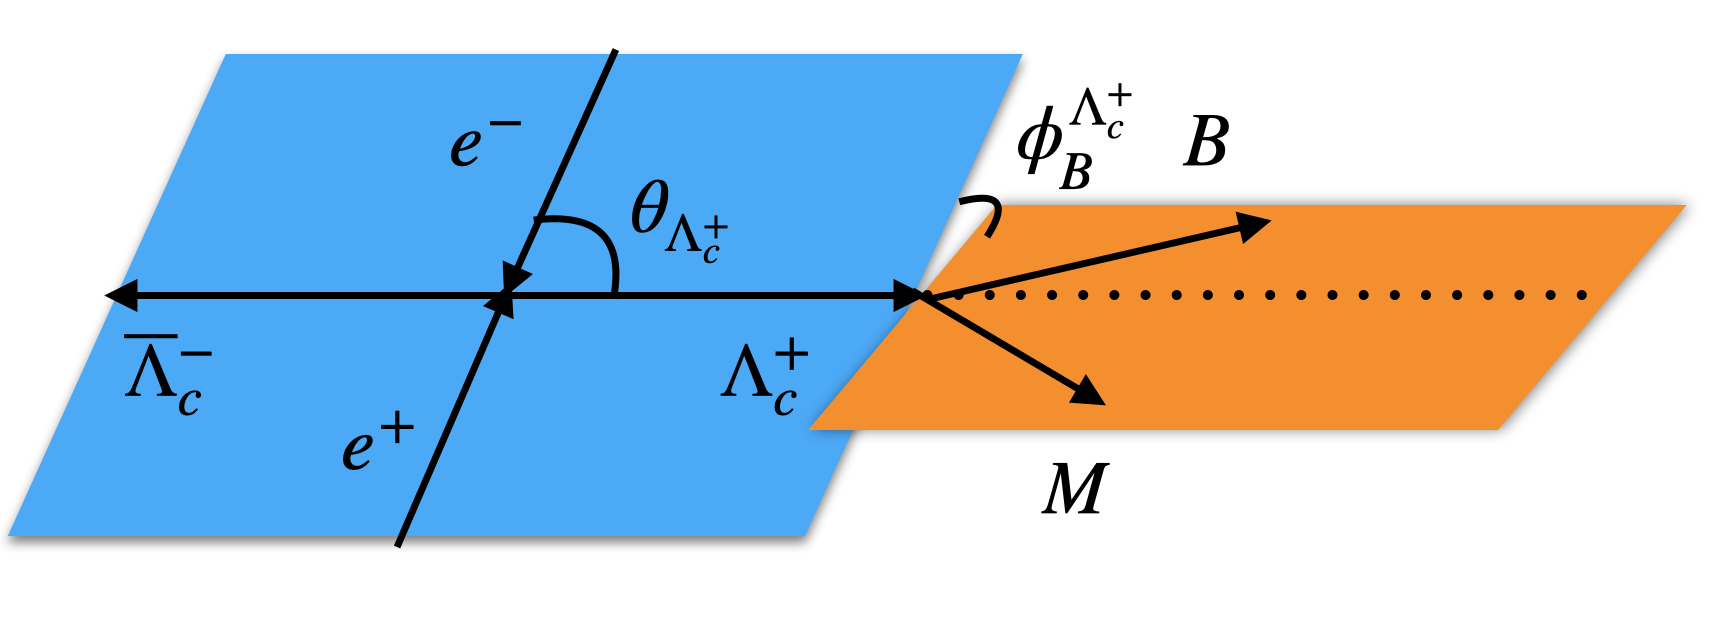
\includegraphics[width=0.50\textwidth]{figure/helicity.png}
    \caption{Definition of helicity angle in the process of $e^+e^- \to \lcp\lcm$ and $\lcp \to BM$. $B$ and $M$ denotes baryon and meson in the decay of $\lcp$. $\theta_{\lcp}$ is the angle between the $\lcp$ and $e^+e^-$ in the rest frame of $e^+e^-$. $\phi_{B}^{\lcp}$ is the angle between the production plane of $\lcp$ and plane determined by the decay products of $\lcp$.} 
    \label{fig:helicity_ee_lclp}
\end{figure}

In this analysis, we perform a amplitude analysis for $e^+e^- \to \lcp\lcm$, $\lcp \to p K^- \pi^+$ and $\lcm$ decays inclusively, using data samples collected at thirteen center-of-mass energies from 4.600 to 4.951 GeV with the BESSIII detector at BEPCII. The charge conjugation is always implied. The transverse polarization parameters, $\alpha_0$ and $\sin\Delta_0$ are obtained at each energy points. Based on the amplitude analysis results of $\lcp \to pK^-\pi^+$, the composition of the resonance structures are obtained in the $pK^-\pi^+$ final state. The decay asymmetry parameters of quasi-two-body $\lcp$ decay are also provided.

\clearpage
\section{BEPCII and BESIII detector}
\label{sec:detector}

The BESIII detector is an approximately cylindrically symmetric detector with 93\% coverage of the solid angle around the $e^+e^-$ interaction point (IP). The components of the apparatus, ordered by distance from the IP, are a 43-layer small-cell main drift chamber (MDC), a time of-flight (TOF) system based on plastic scintillators with two layers in the barrel region and one layer in the end-cap region (the end-cap TOF system has been updated with the multi-gap resistive plate chamber in 2014~\cite{Yang:2014pfa}), a 6240-cell CsI(Tl) crystal electromagnetic calorimeter (EMC), a superconducting solenoid magnet providing a 1.0 T magnetic field aligned with the beam axis, and resistive plate muon-counter layers interleaved with steel. The momentum resolution for charged tracks in the MDC is 0.5\% for transverse momenta with 1 $\gev$. The energy resolution in the EMC is 2.5\% in the barrel region and 5.0\% in the end-cap region for  1 GeV photons. For charged tracks, particle identification (PID) for charged tracks combines measurements of the energy deposit d$E$/d$x$ in MDC and flight time in TOF and forms likelihoods $\mathcal{L}(h)(h = K, \pi)$ for a hadron h hypothesis. More details about the BESIII detector are provided in Ref.~\cite{BESIII:2009fln}.

\clearpage
\section{Data and MC samples}
\label{sec:sample}
This analysis uses a combined data sample with a integrated luminosity of 6.4 fb$^{-1}$ collected at 13 c.m. energy points from $\sqrt{s}=4.600~\gev$ to 4.951~$\gev$, which are reconstructed under BOSS version of 7.0.6 and 7.0.7. More details about these data samples are listed in Table~\ref{tab:datainfo}.

\begin{table}[htbp]
    \centering
    \caption{The c.m. energy ($E_{\rm cms}$), the integrated luminosity, and BOSS version of the data samples in this analysis~\cite{BESIII:2015qfd,BESIII:2015zbz,BESIII:2022dxl,BESIII:2022ulv}.}
    \begin{tabular}{cccc}\hline\hline
        Sample  &  $\sqrt{s}$ (MeV) & $\mathcal{L}_{\rm int}$ (pb$^{-1}$)  & BOSS version \\\hline
        4600    & 4599.53 $\pm$ 0.07 $\pm$ 0.74 & 586.9 $\pm$ 0.1 $\pm$ 3.9 & \multirow{7}{4em}{7.0.6}\\
        4612    & 4611.86 $\pm$ 0.12 $\pm$ 0.30 & 103.65 $\pm$ 0.05 $\pm$ 0.55 \\
        4626    & 4628.00 $\pm$ 0.06 $\pm$ 0.32 & 521.53 $\pm$ 0.11 $\pm$ 2.76 \\
        4640    & 4640.91 $\pm$ 0.06 $\pm$ 0.29 & 551.65 $\pm$ 0.12 $\pm$ 2.92 \\
        4660    & 4661.24 $\pm$ 0.06 $\pm$ 0.29 & 529.43 $\pm$ 0.12 $\pm$ 2.81\\
        4680    & 4681.92 $\pm$ 0.08 $\pm$ 0.29 & 1667.39 $\pm$ 0.21 $\pm$ 8.84\\
        4700    & 4698.82 $\pm$ 0.10 $\pm$ 0.36 & 535.54 $\pm$ 0.12 $\pm$ 2.84 \\\hline
        4740    & 4739.70 $\pm$ 0.20 $\pm$ 0.30 & 163.87 $\pm$ 0.07 $\pm$ 0.87 & \multirow{6}{4em}{7.0.7}\\
        4750    & 4750.05 $\pm$ 0.12 $\pm$ 0.29 & 366.55 $\pm$ 0.10 $\pm$ 1.94 \\
        4780    & 4780.54 $\pm$ 0.12 $\pm$ 0.30 & 511.47 $\pm$ 0.12 $\pm$ 2.71 \\
        4840    & 4843.07 $\pm$ 0.20 $\pm$ 0.31 & 525.16 $\pm$ 0.12 $\pm$ 2.78 \\
        4920    & 4918.02 $\pm$ 0.34 $\pm$ 0.34 & 207.82 $\pm$ 0.08 $\pm$ 1.10\\
        4950    & 4950.93 $\pm$ 0.36 $\pm$ 0.38 & 159.28 $\pm$ 0.07 $\pm$ 0.84\\
        \hline\hline
    \end{tabular}
    \label{tab:datainfo}
\end{table}

Simulated samples are produced using a \textsc{Geant4}-based~\cite{GEANT4:2002zbu} Monte Carlo (MC) packages, which includes the geometric descriptions of the BESIII detector~\cite{Liang:2009zzb,Huang:2022wuo} and detector response. The beam-energy spread and initial-state radiation (ISR) in the $e^+e^-$ annihilation are simulated with the \textsc{KKMC} generator~\cite{Jadach:2000ir} in the MC samples. The final-state radiation (FSR) from the charged particles are modeled using \textsc{PHOTOS}~\cite{Richter-Was:1992hxq}. Three kinds of MC samples are used in ths analysis as described below:
\begin{itemize}
    \item Cocktail MC samples:
    \begin{itemize}
        \item Inclusive $\lcp\lcm$ MC samples, which simulate the production of $\lcp\lcm$ pairs. The cross section of $e^+e^- \to \lcp\lcm$ process is based on the analysis of Ref~\cite{Wang:memo}, and the subsequent decay modes of $\lcp(\lcm)$ are inclusive using the branching fractions (BFs) taken from the PDG~\cite{Workman:2022ynf}. The integrated luminosity is 40 times larger than that of data. These samples are used to study the background contribution from $\lcp\lcm$ pair production in data. 
        \item Inclusive hadron MC samples, which includes open-charmed mesons, ISR production of vector charmonium(-like) states and continuum processes. The known decay modes are modelled with \textsc{Evtgen}~\cite{Lange:2001uf,Ping:2008zz} using the BFs taken from the PDG~\cite{Workman:2022ynf}. The remaining unknown decays are simulated with \textsc{LUNDCHARM}~\cite{Chen:2000tv,Yang:2014vra}. The integrated luminosity is 10 times larger than that of data. These samples are used to study the background contribution from non-$\lcp\lcm$ pair production in data. 
    \end{itemize}
    \item Invisible PHSP signal MC samples, in which the signal process $\lcp \to pK^-\pi^+$ is generated with a uniform phase-space (PHSP) distribution and $\lcm$ decays into invisible particle which does not interact with the detector. 200K signal MC events are generated at each energy point, except for 400K events at $\sqrt{s} = 4.682~\gev$ due to its large integrated luminosity. The invisible signal MC samples are used to extract the pure signal shape, which will be used in the fit to the $\mbc$ distributions.
    \item Inclusive PHSP signal MC samples are produced with the same decay mode for the $\lcp$ in the signal side. For the other $\lcm$, it is required to inclusively decay to all possible final states with the BFs and models following the official DECAY.DEC file in the BesEvtGen package. The numbers of produced events are the same as the invisible signal MC samples. The inclusive signal MC samples are used in the MC integration part to construct the likelihood of the amplitude analysis with detection efficiencies automatically taken into account. 
    %The effects of MC statistics are studied and found to be small in the amplitude analysis, documented in Appendix~\ref{app:mc_statistics}.
\end{itemize}

\clearpage
\section{Event selections}
\label{sec:selections}

Based on the $\lcp\lcm$ pair production and the excellent performance of the BESIII detector, the single-tag (ST) method is utilized to selectively identify one of the charmed baryons. This approach yields a substantial data sample with a high selection efficiency. 

\subsection{General selections}
\label{sec:general_cuts}
The signal candidates of $\lcp(\lcm)$ are reconstructed from three charged tracks: proton, kaon and pion, which satisfy the following criteria. 
\begin{itemize}
    \item Good charged tracks: \\
    A charged track is taken as a good MDC track if it originates from the beam vertex and lies within the MDC polar angle region.
    \begin{itemize}
        \item $|\cos\theta|<0.93$, where $\theta$ is the polar angle with respect to the beam axis.
        \item $|\Delta r|<1~\unit{cm}$, $|\Delta z|<10\,\unit{cm}$, where $|\Delta r|$ and $|\Delta z|$ is distance of closest approach to the interaction point (IP) perpendicular to the beam axis and along the beam axis, respectively.
    \end{itemize}
    
    \item Particle identifications: \\
    Particle identification (PID) algorithm is employed to separate proton, kaon and pion, combining d$E/$d$x$ and TOF information.
    \begin{itemize}
        \item $p$ PID requirements:  $\mathcal{L}(p)>0$ $\mathcal{\&\&}$ $\mathcal{L}(p)>\mathcal{L}(K)$ $\mathcal{\&\&}$ $\mathcal{L}(p)>\mathcal{L}(\pi)$.
        \item $K$ PID requirements: $\mathcal{L}(K)>0$ $\mathcal{\&\&}$ $\mathcal{L}(K)>\mathcal{L}(\pi)$.
        \item $\pi$ PID requirements:  $\mathcal{L}(\pi)>0$ $\mathcal{\&\&}$ $\mathcal{L}(\pi)>\mathcal{L}(K)$
    \end{itemize}
\end{itemize}

The energy difference is calculated using $\dE=E-\ebeam$, where $E$ represents the total reconstructed energy of the $\lcp$ candidate, and $\ebeam$ corresponds to the mean value of the $e^+$ and $e^-$ beams in the c.m. frame of the $e^+e^-$ collision. A correctly reconstructed $\lcp$ candidate should exhibit a peak around zero in the $\dE$ distribution. To prevent double counting in each event, the signal candidate with the smallest $\dE$ value is selected. Furthermore, an additional requirement on $\dE$ within the range of $(-0.029, 0.026)\gev$, identical to that in Ref.~\cite{BESIII:2022xne}, is applied. This criterion ensures the inclusion of at least 97\% of the signal events while effectively rejecting background events.

The beam-constrained mass, denoted as $\mbc$, is defined by $\mbc = \sqrt{\ebeam^2/c^4 - |\vec{p}|^2/c^2}$, where $\vec{p}$ represents the total reconstructed momentum of the $\lcp$ candidate in the c.m. frame of the $e^+e^-$ collision. A comparison has been conducted between the data and cocktail Monte Carlo (MC) samples regarding the distribution of $\mbc$ for each energy point. This comparison is illustrated in Figure~\ref{fig:full_mbc}. No peaking backgrounds have been observed.

\begin{figure}[h]\centering
    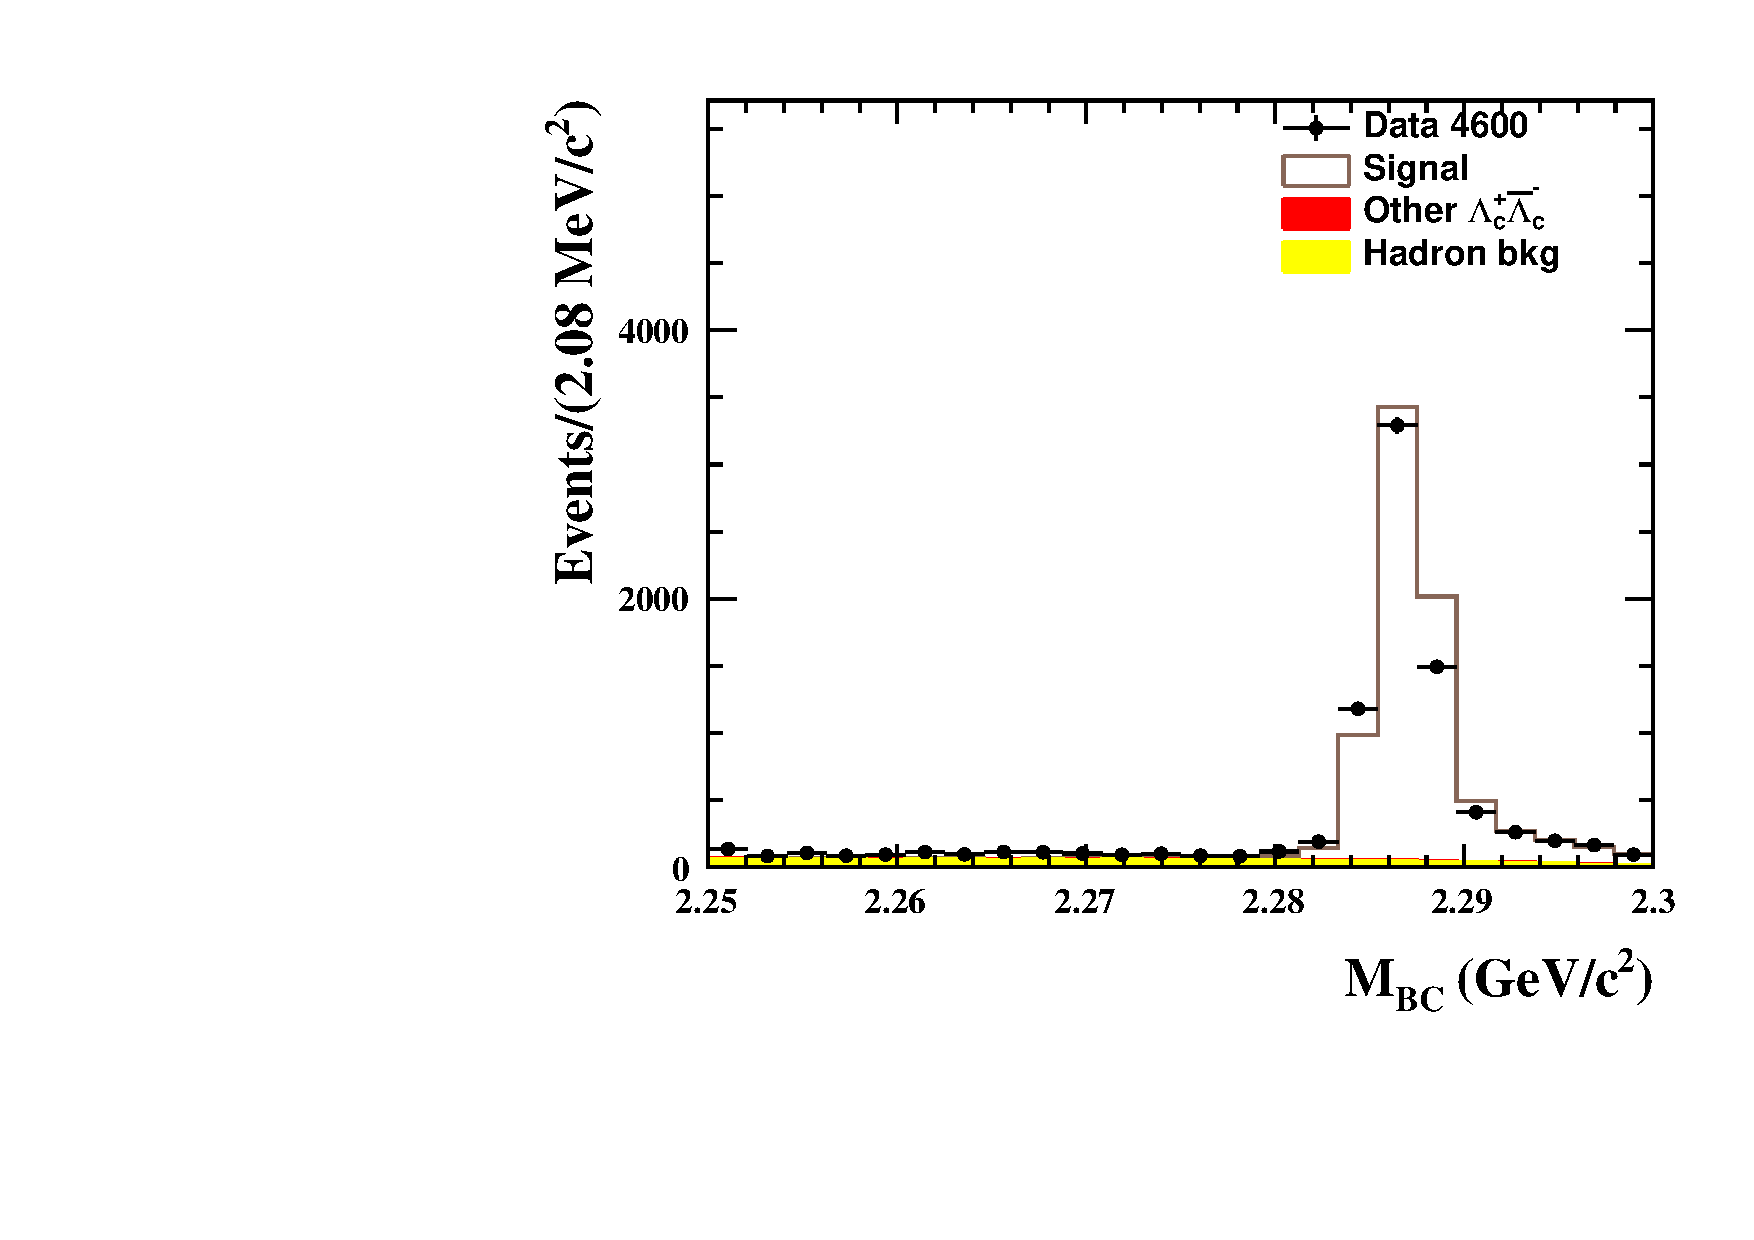
\includegraphics[width=0.24\textwidth]{figure/full_mbc/output_4600_mBC.pdf}
    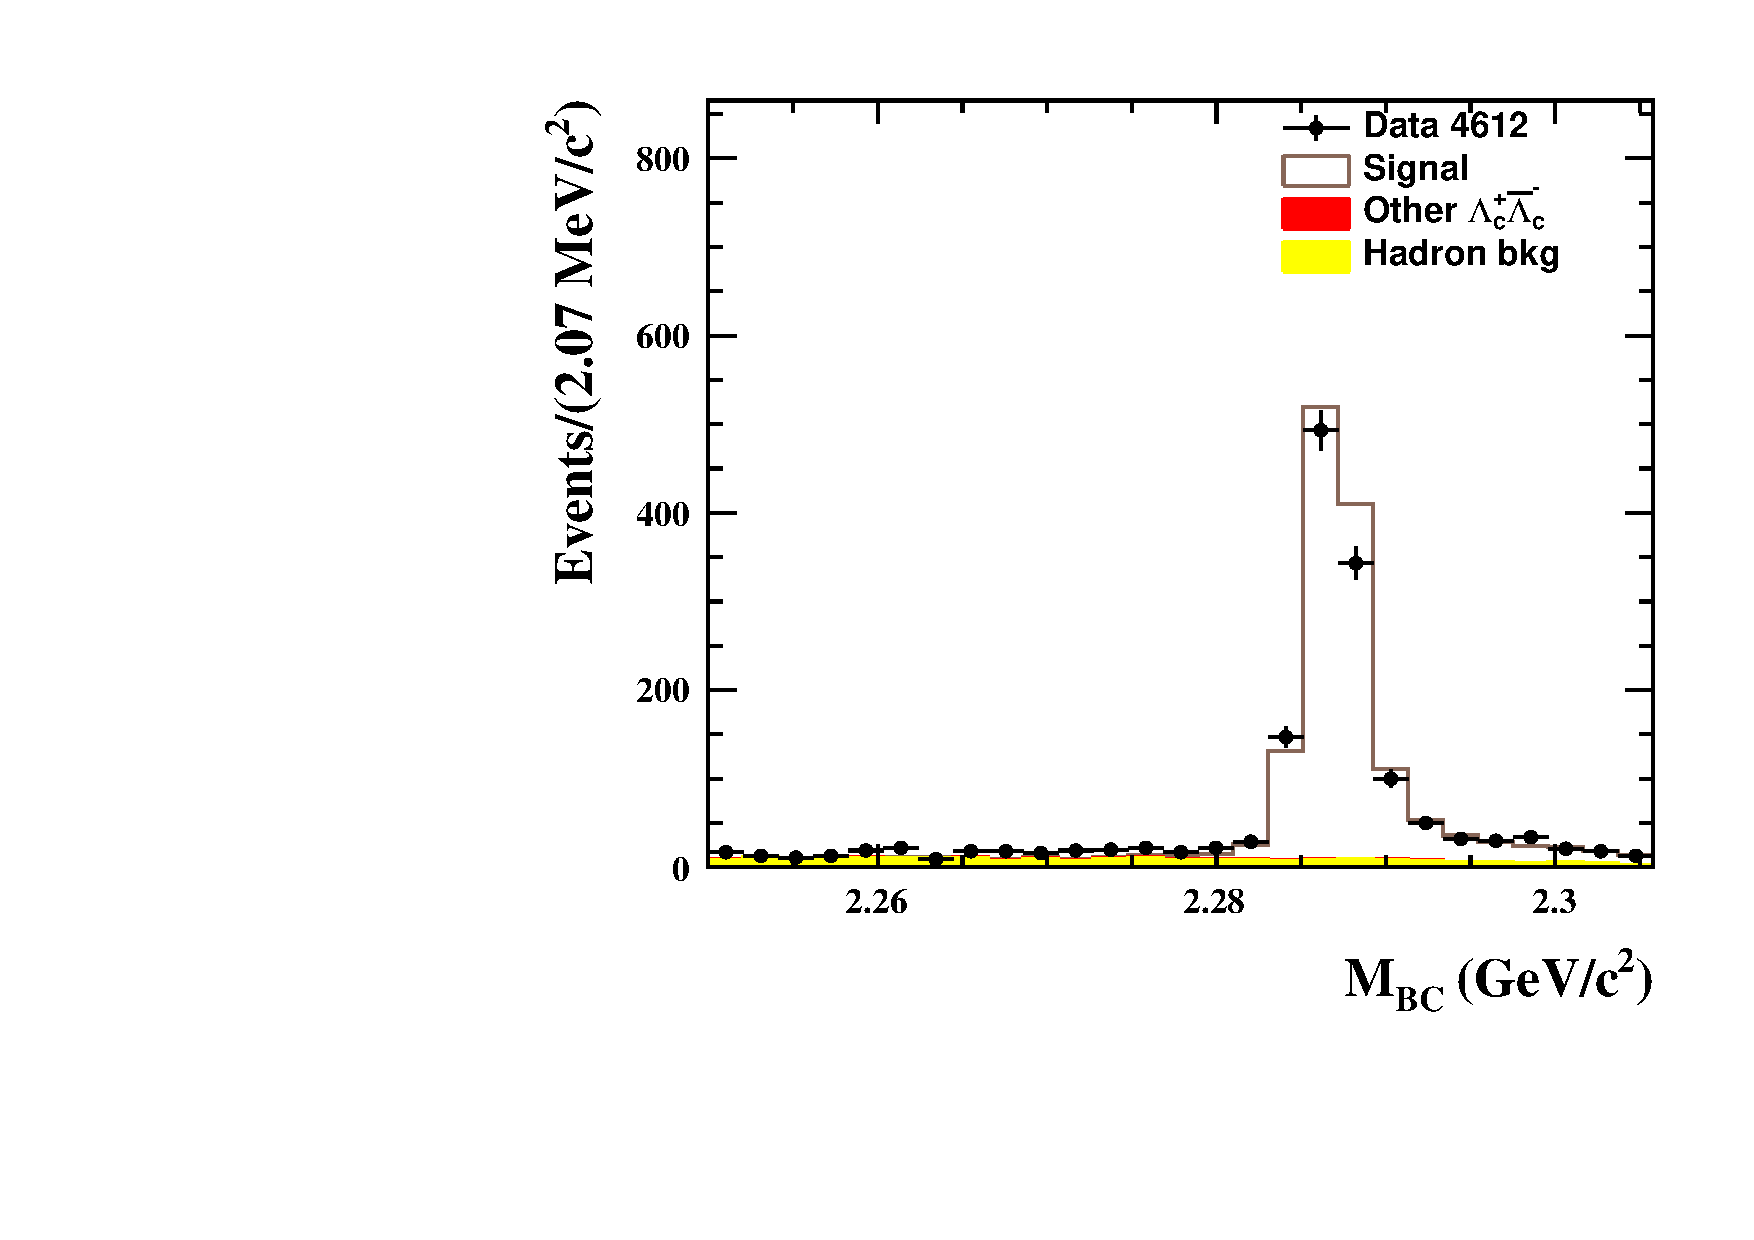
\includegraphics[width=0.24\textwidth]{figure/full_mbc/output_4612_mBC.pdf}
    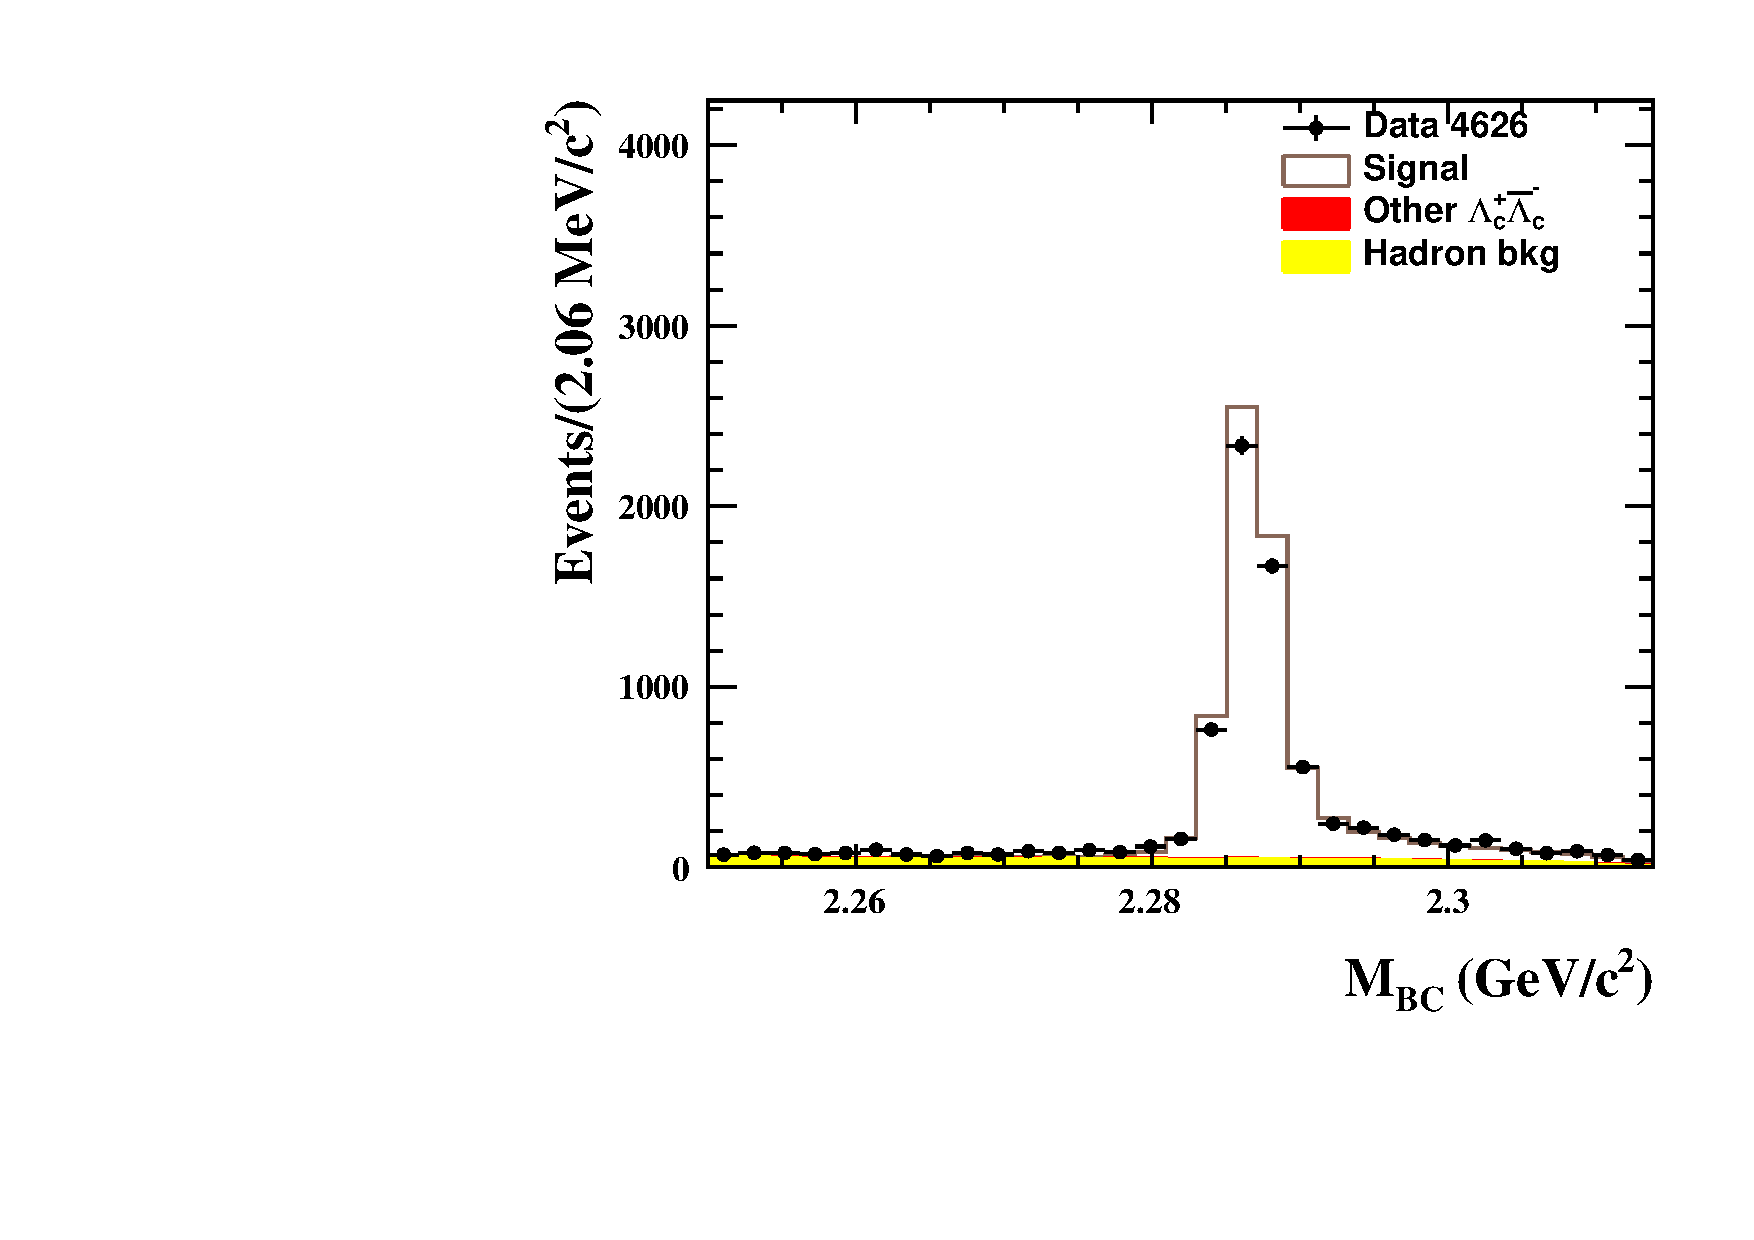
\includegraphics[width=0.24\textwidth]{figure/full_mbc/output_4626_mBC.pdf}
    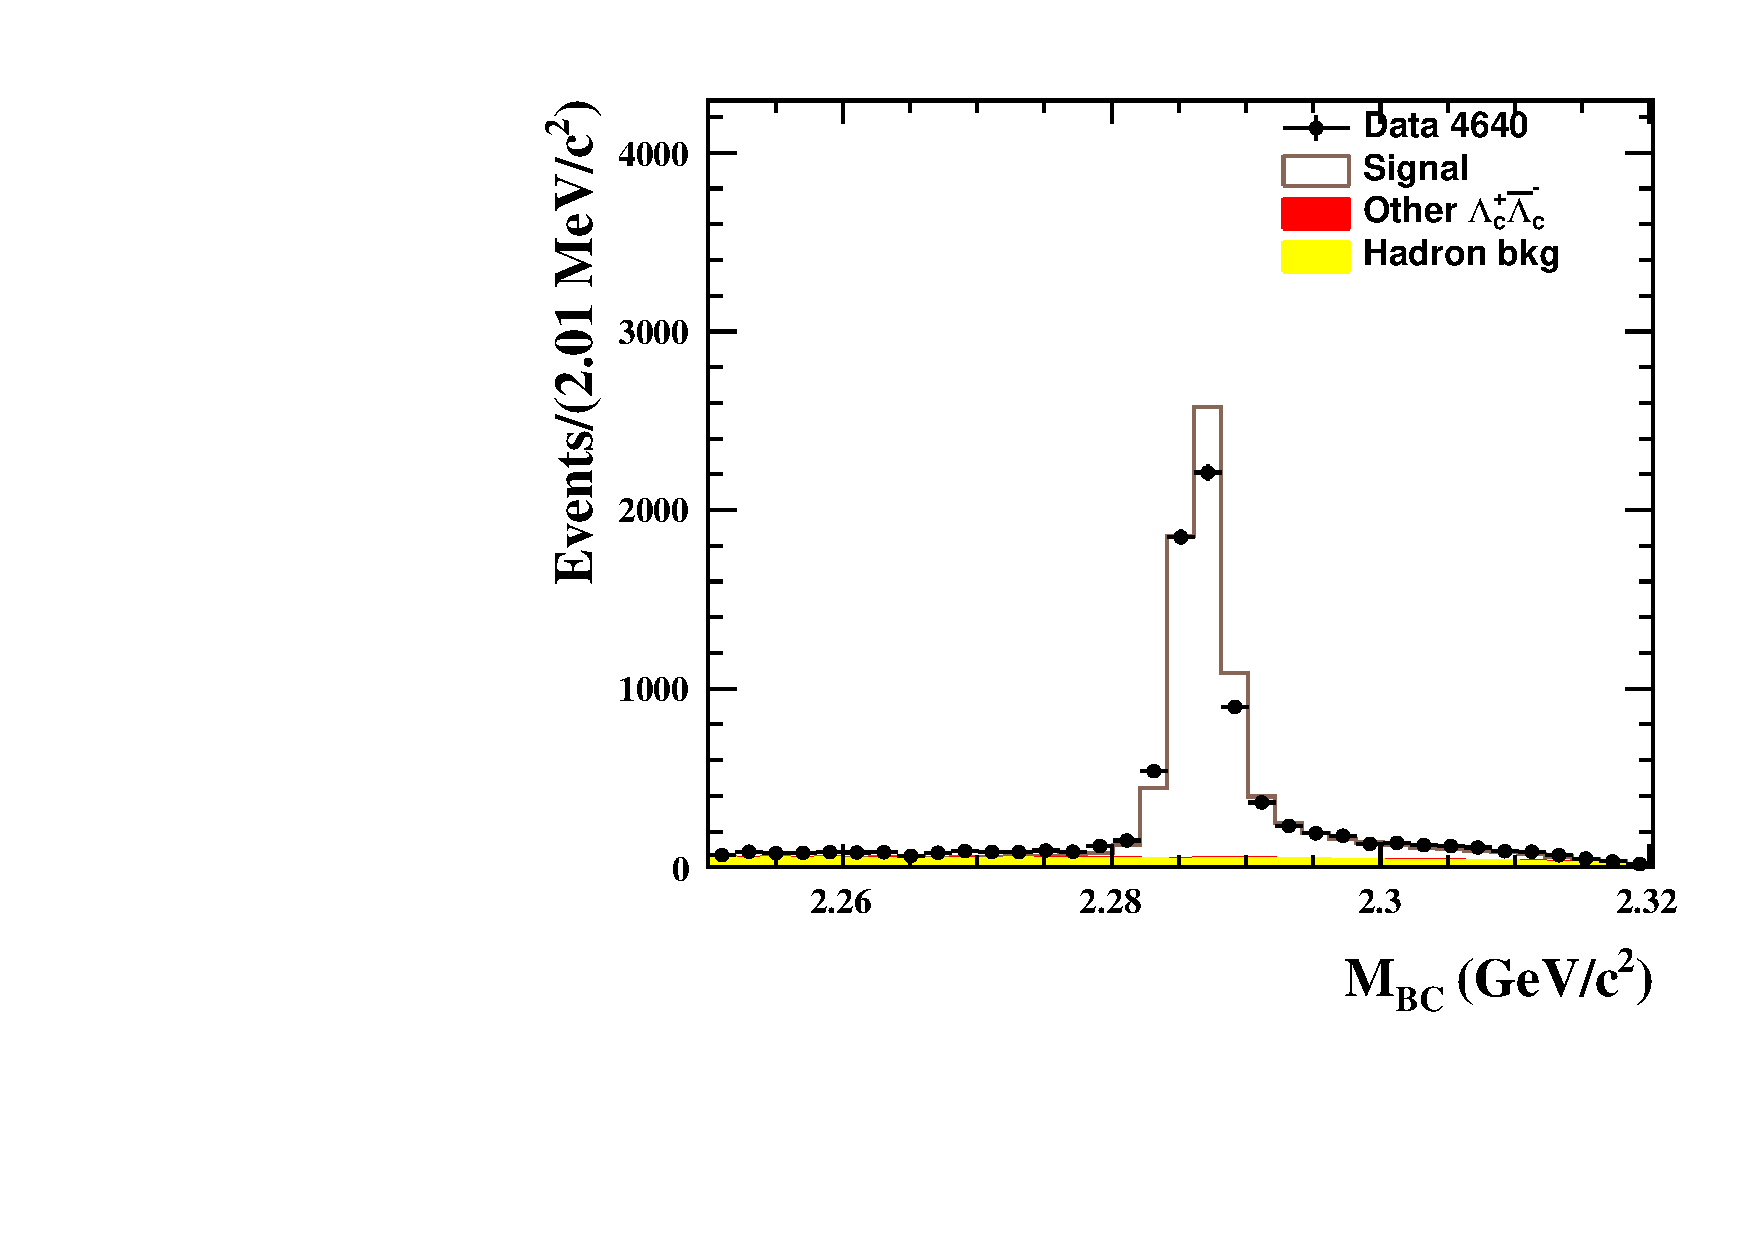
\includegraphics[width=0.24\textwidth]{figure/full_mbc/output_4640_mBC.pdf}
    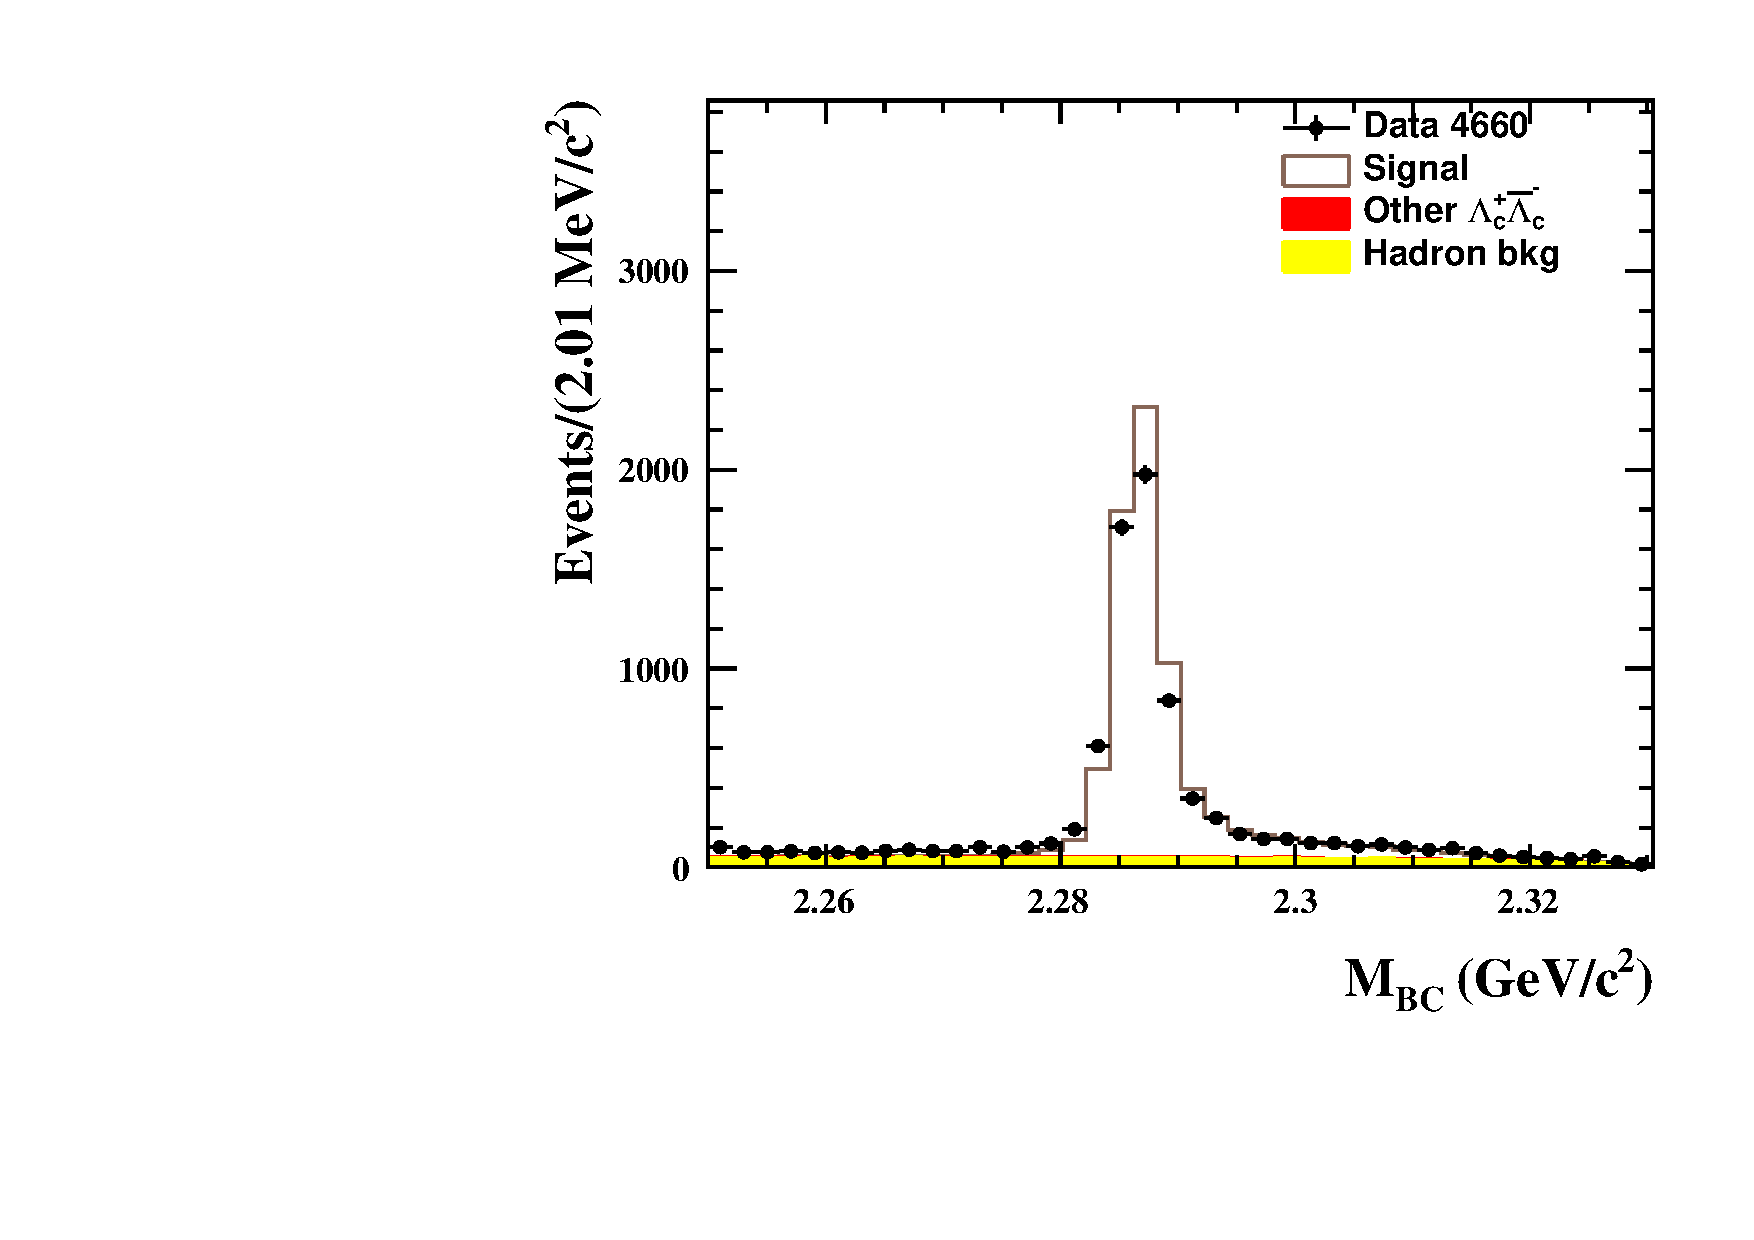
\includegraphics[width=0.24\textwidth]{figure/full_mbc/output_4660_mBC.pdf}
    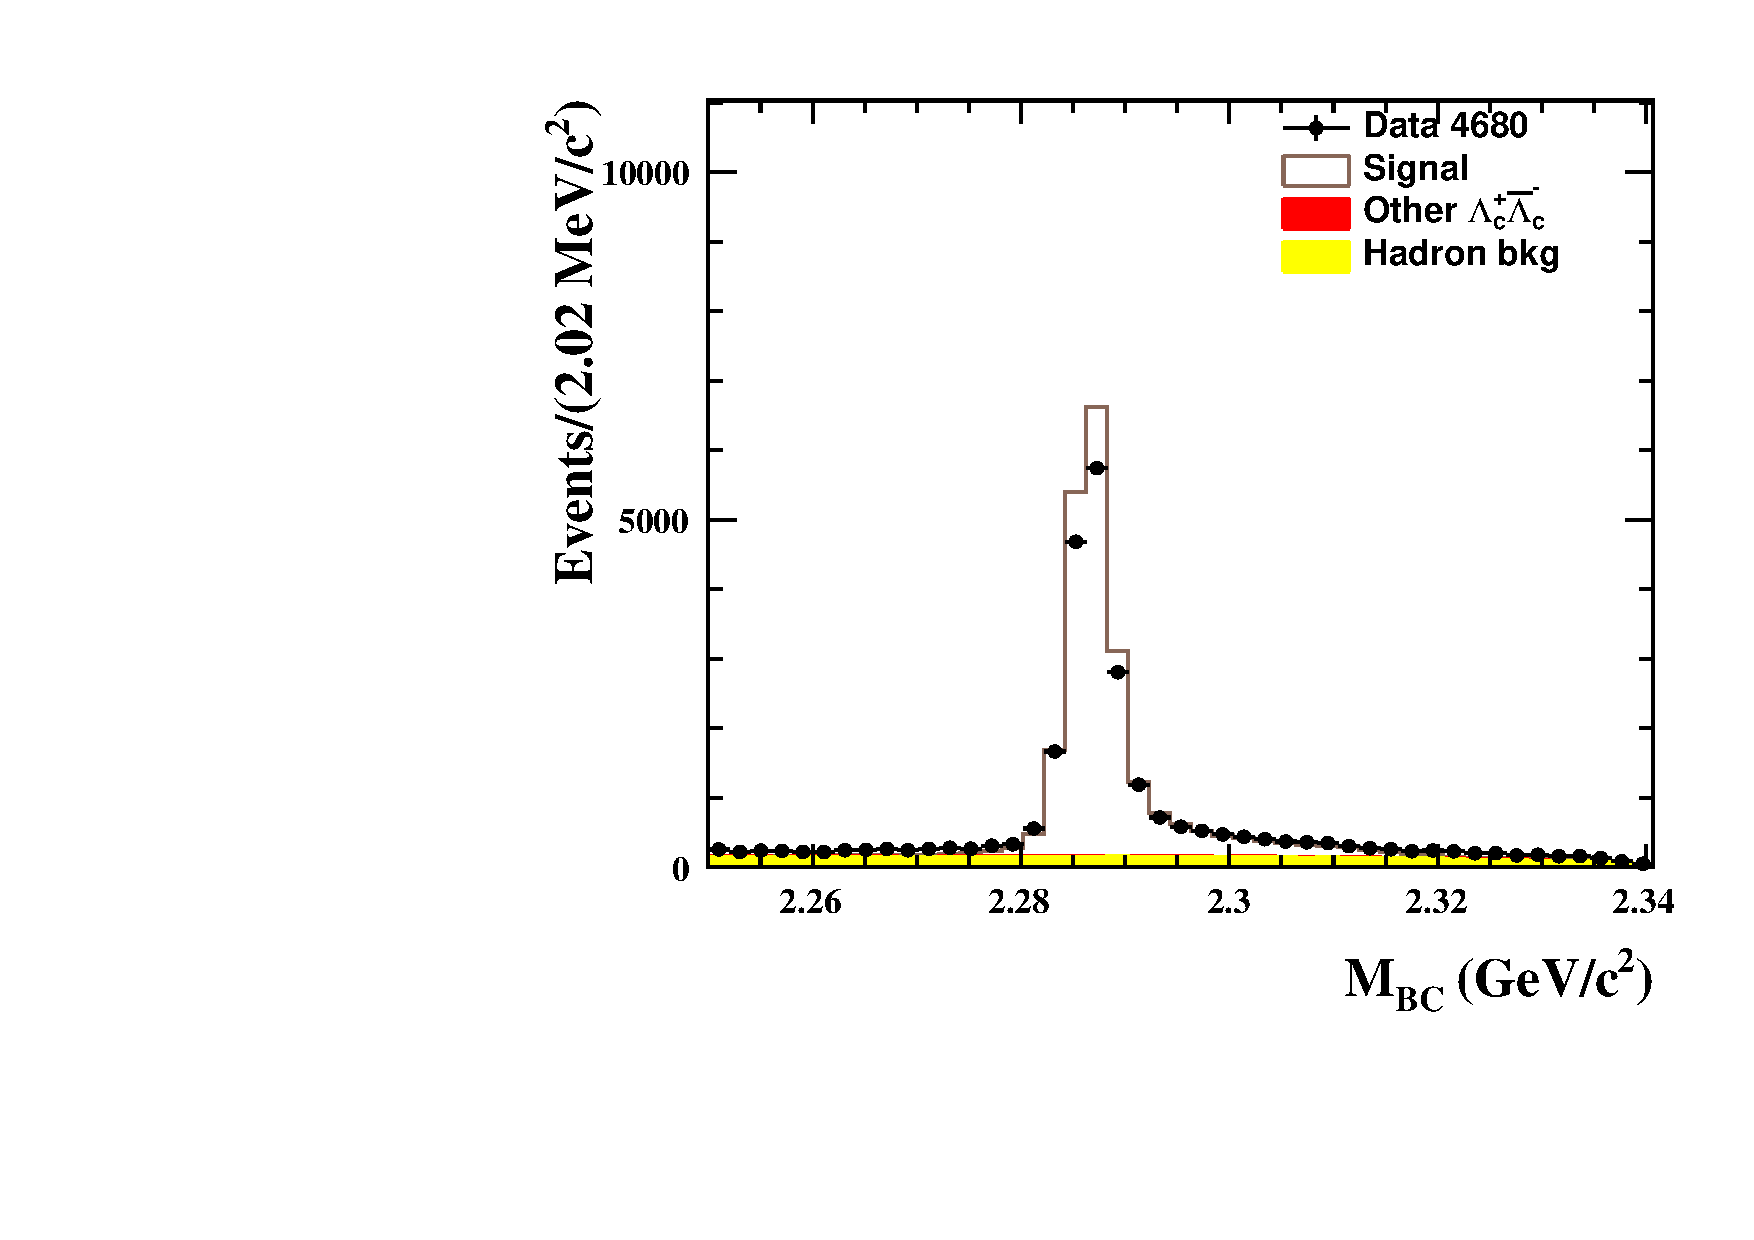
\includegraphics[width=0.24\textwidth]{figure/full_mbc/output_4680_mBC.pdf}
    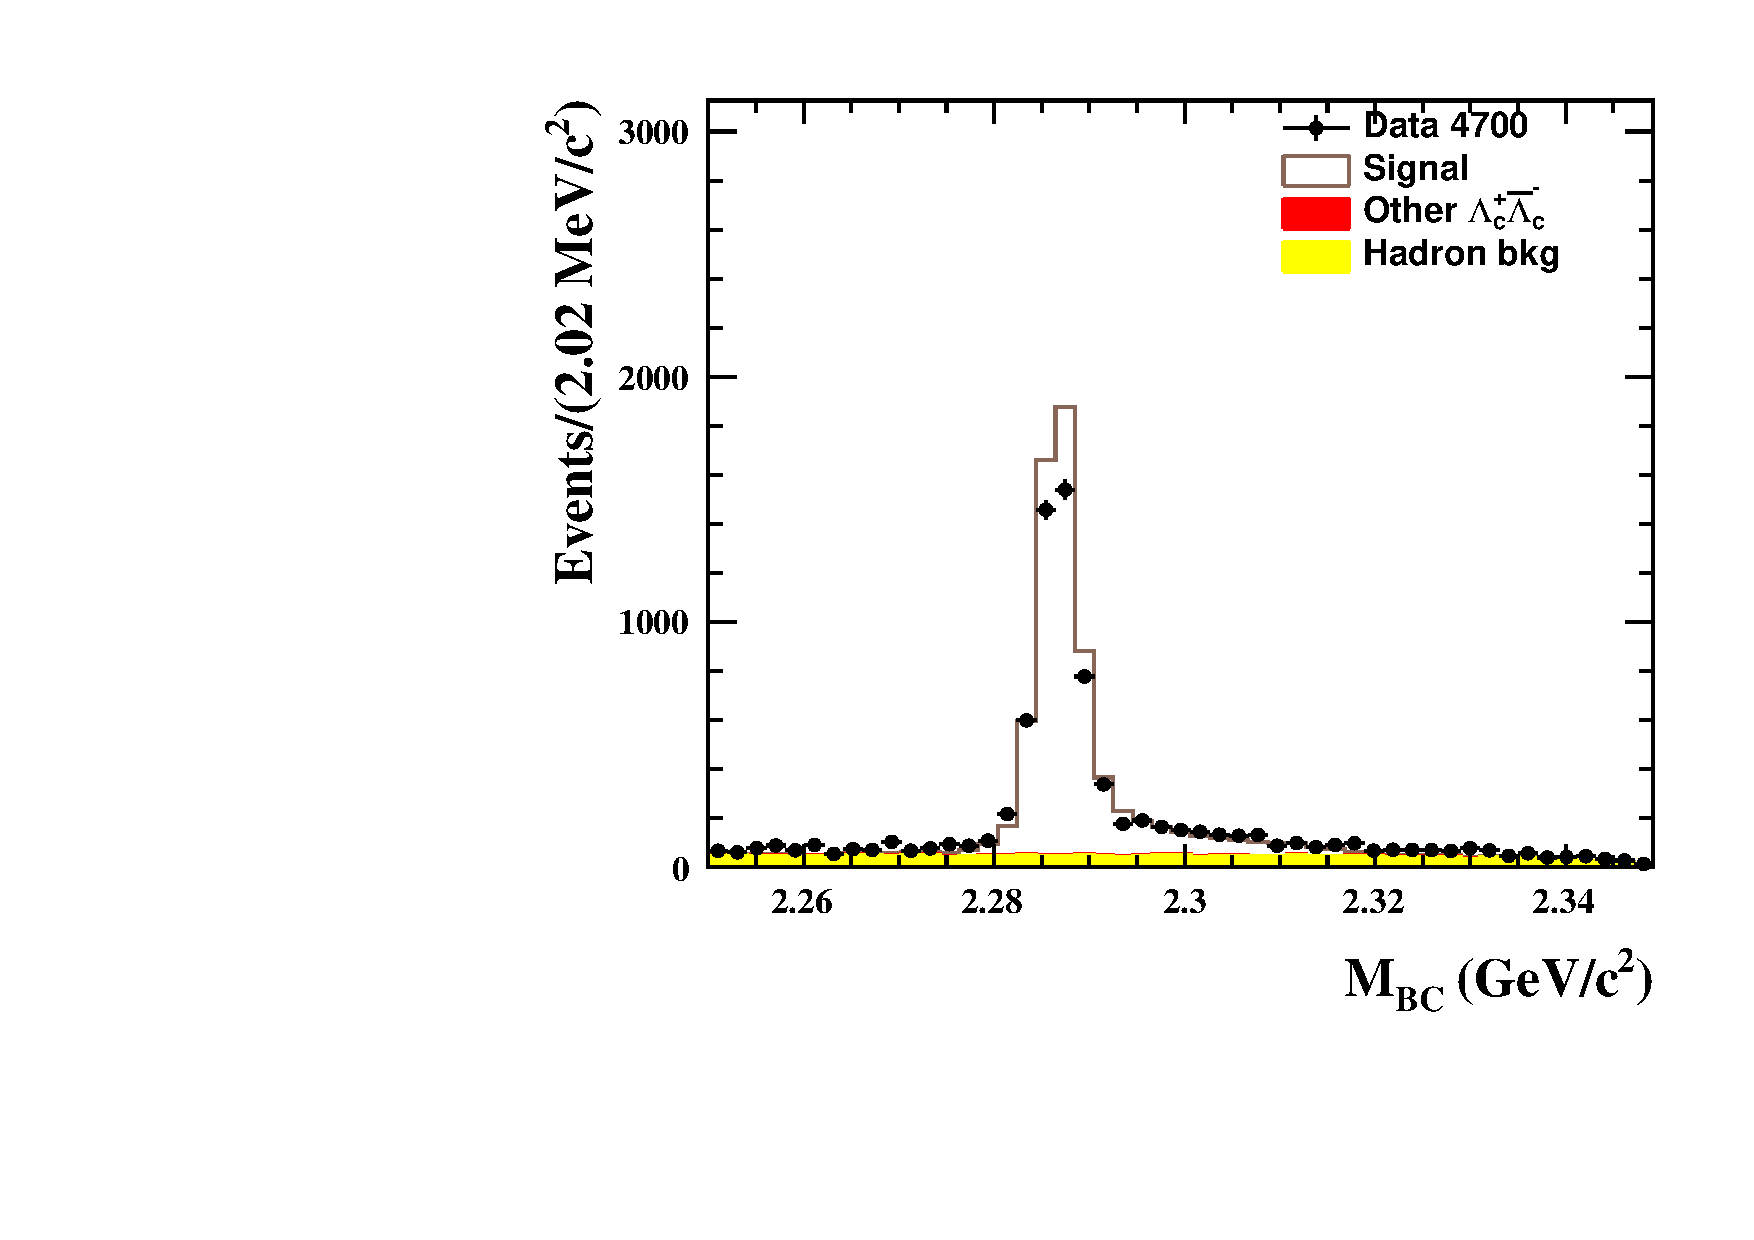
\includegraphics[width=0.24\textwidth]{figure/full_mbc/output_4700_mBC.pdf}
    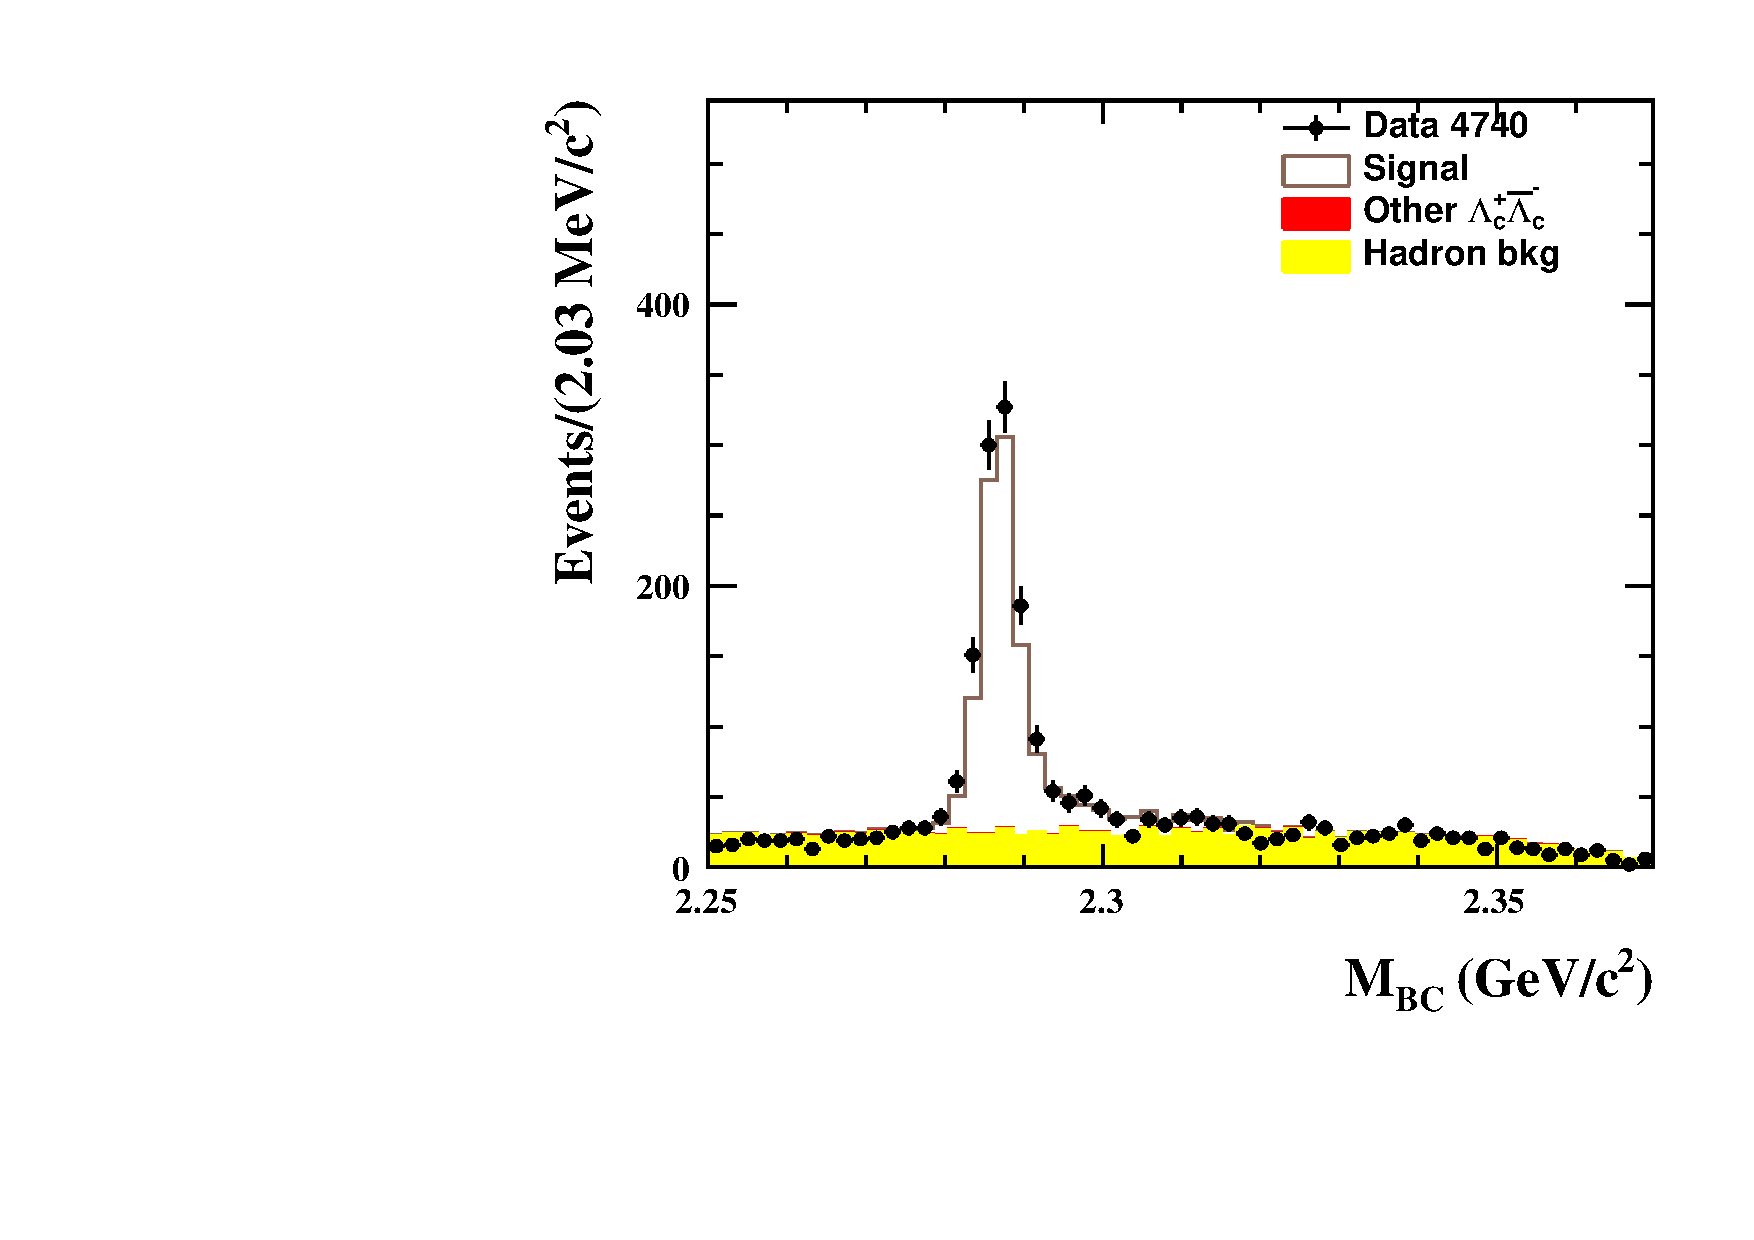
\includegraphics[width=0.24\textwidth]{figure/full_mbc/output_4740_mBC.pdf}
    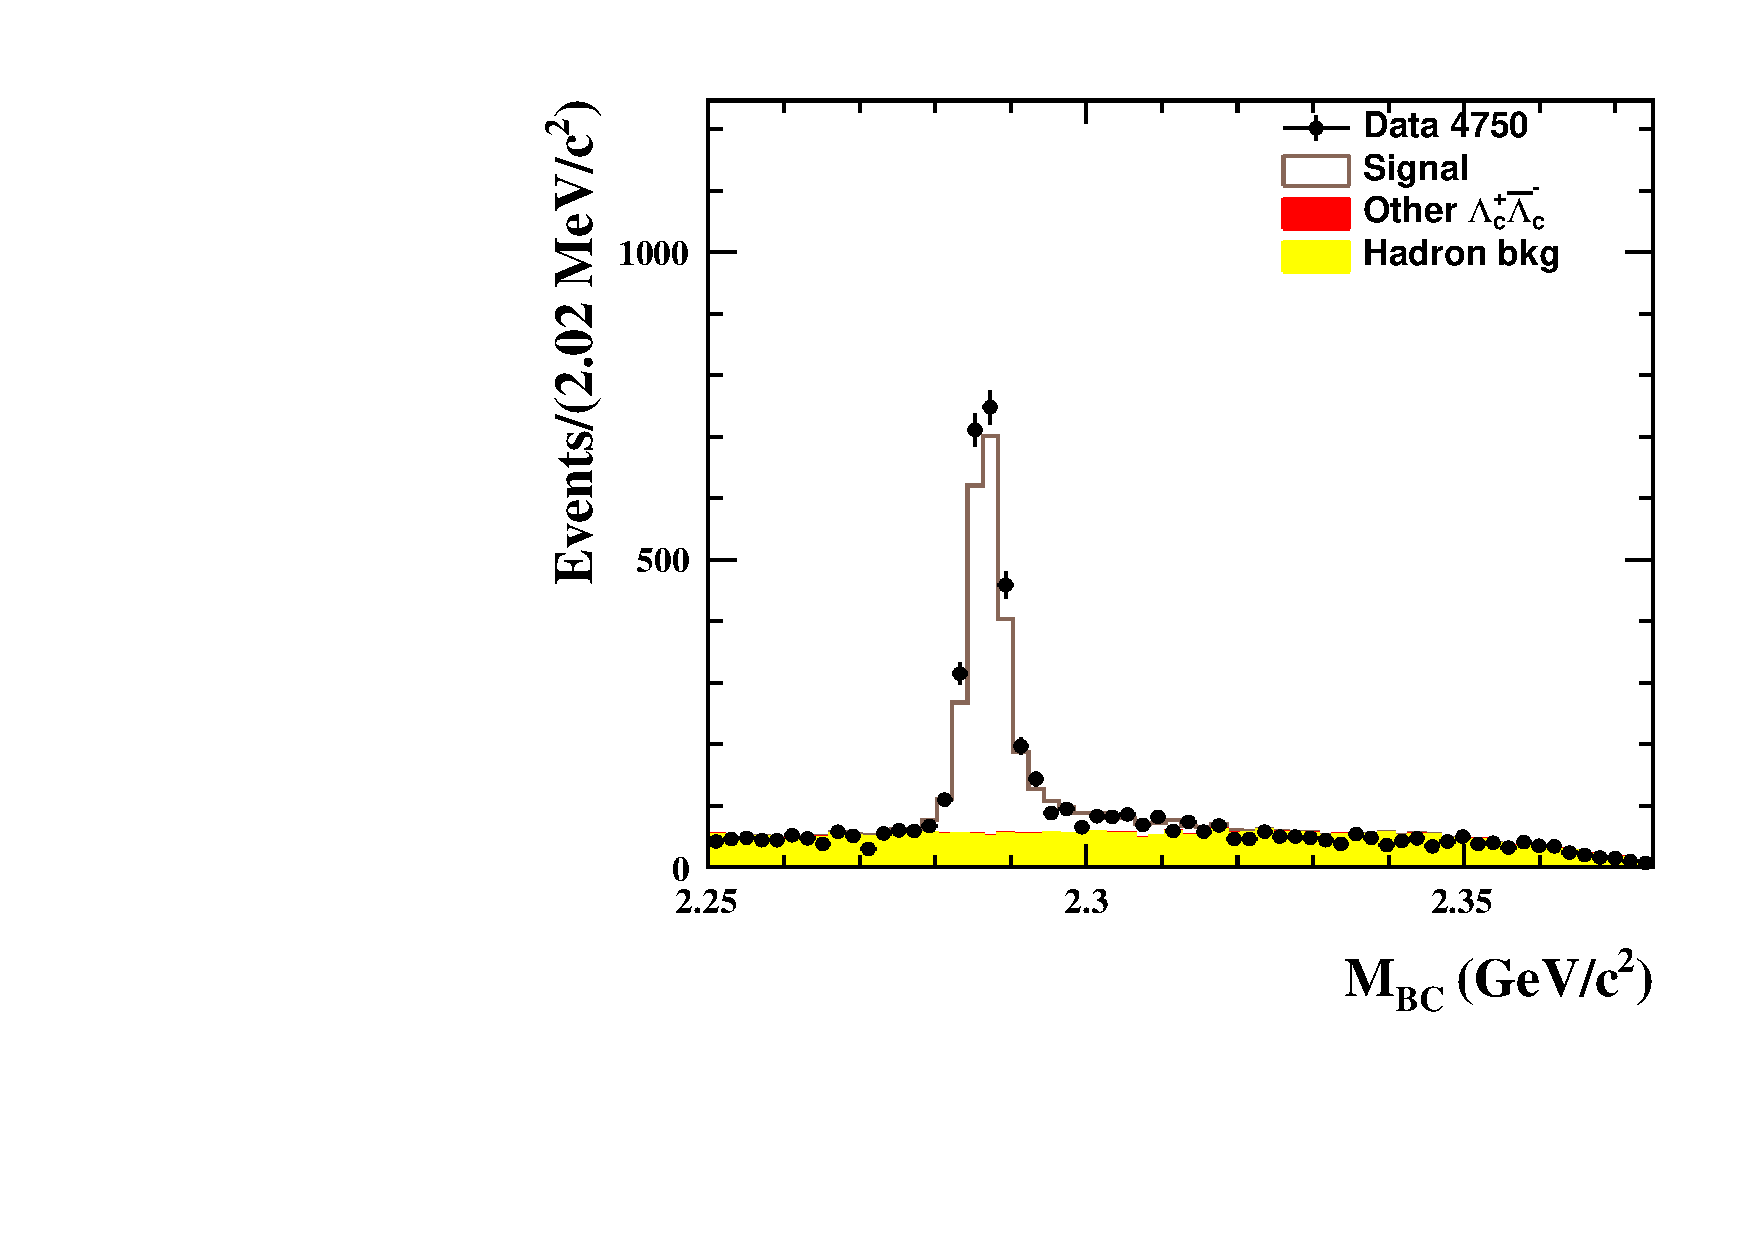
\includegraphics[width=0.24\textwidth]{figure/full_mbc/output_4750_mBC.pdf}
    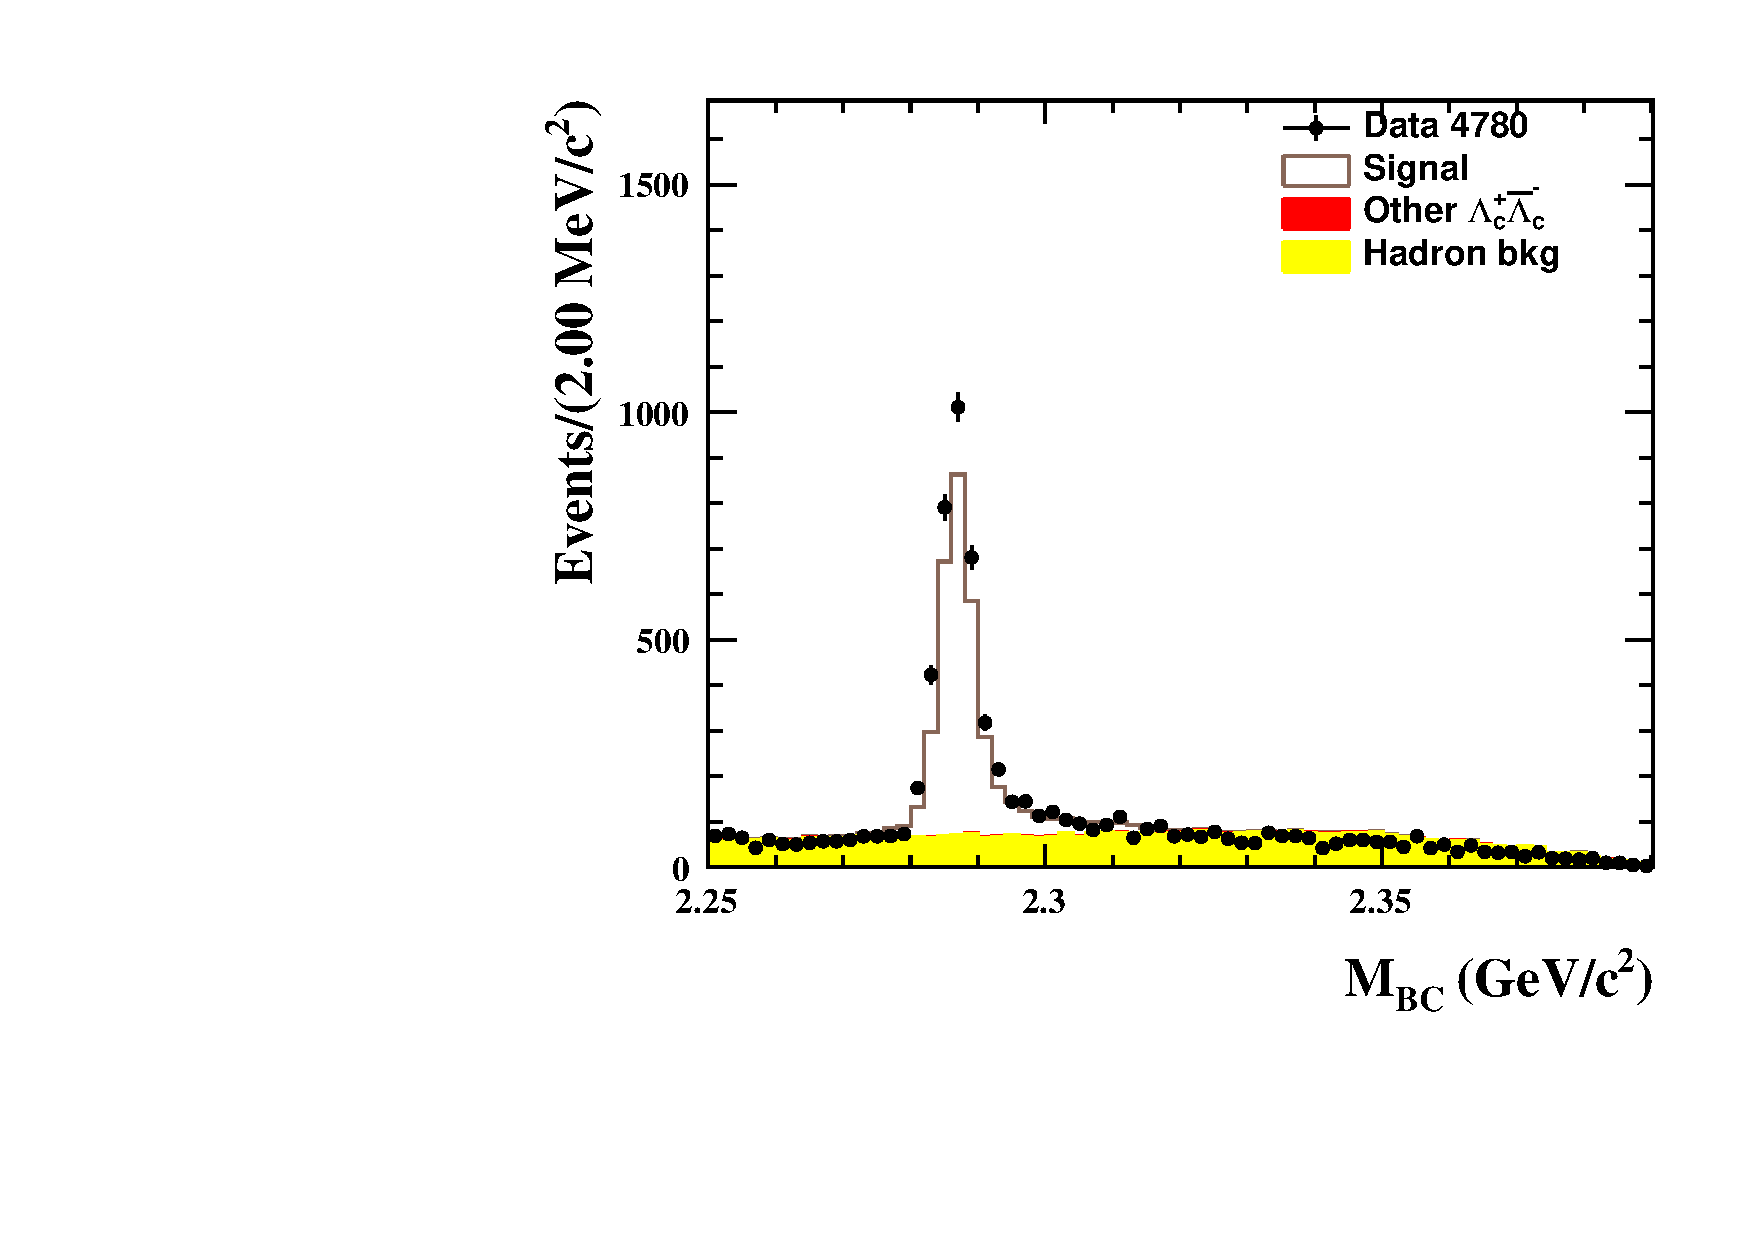
\includegraphics[width=0.24\textwidth]{figure/full_mbc/output_4780_mBC.pdf}
    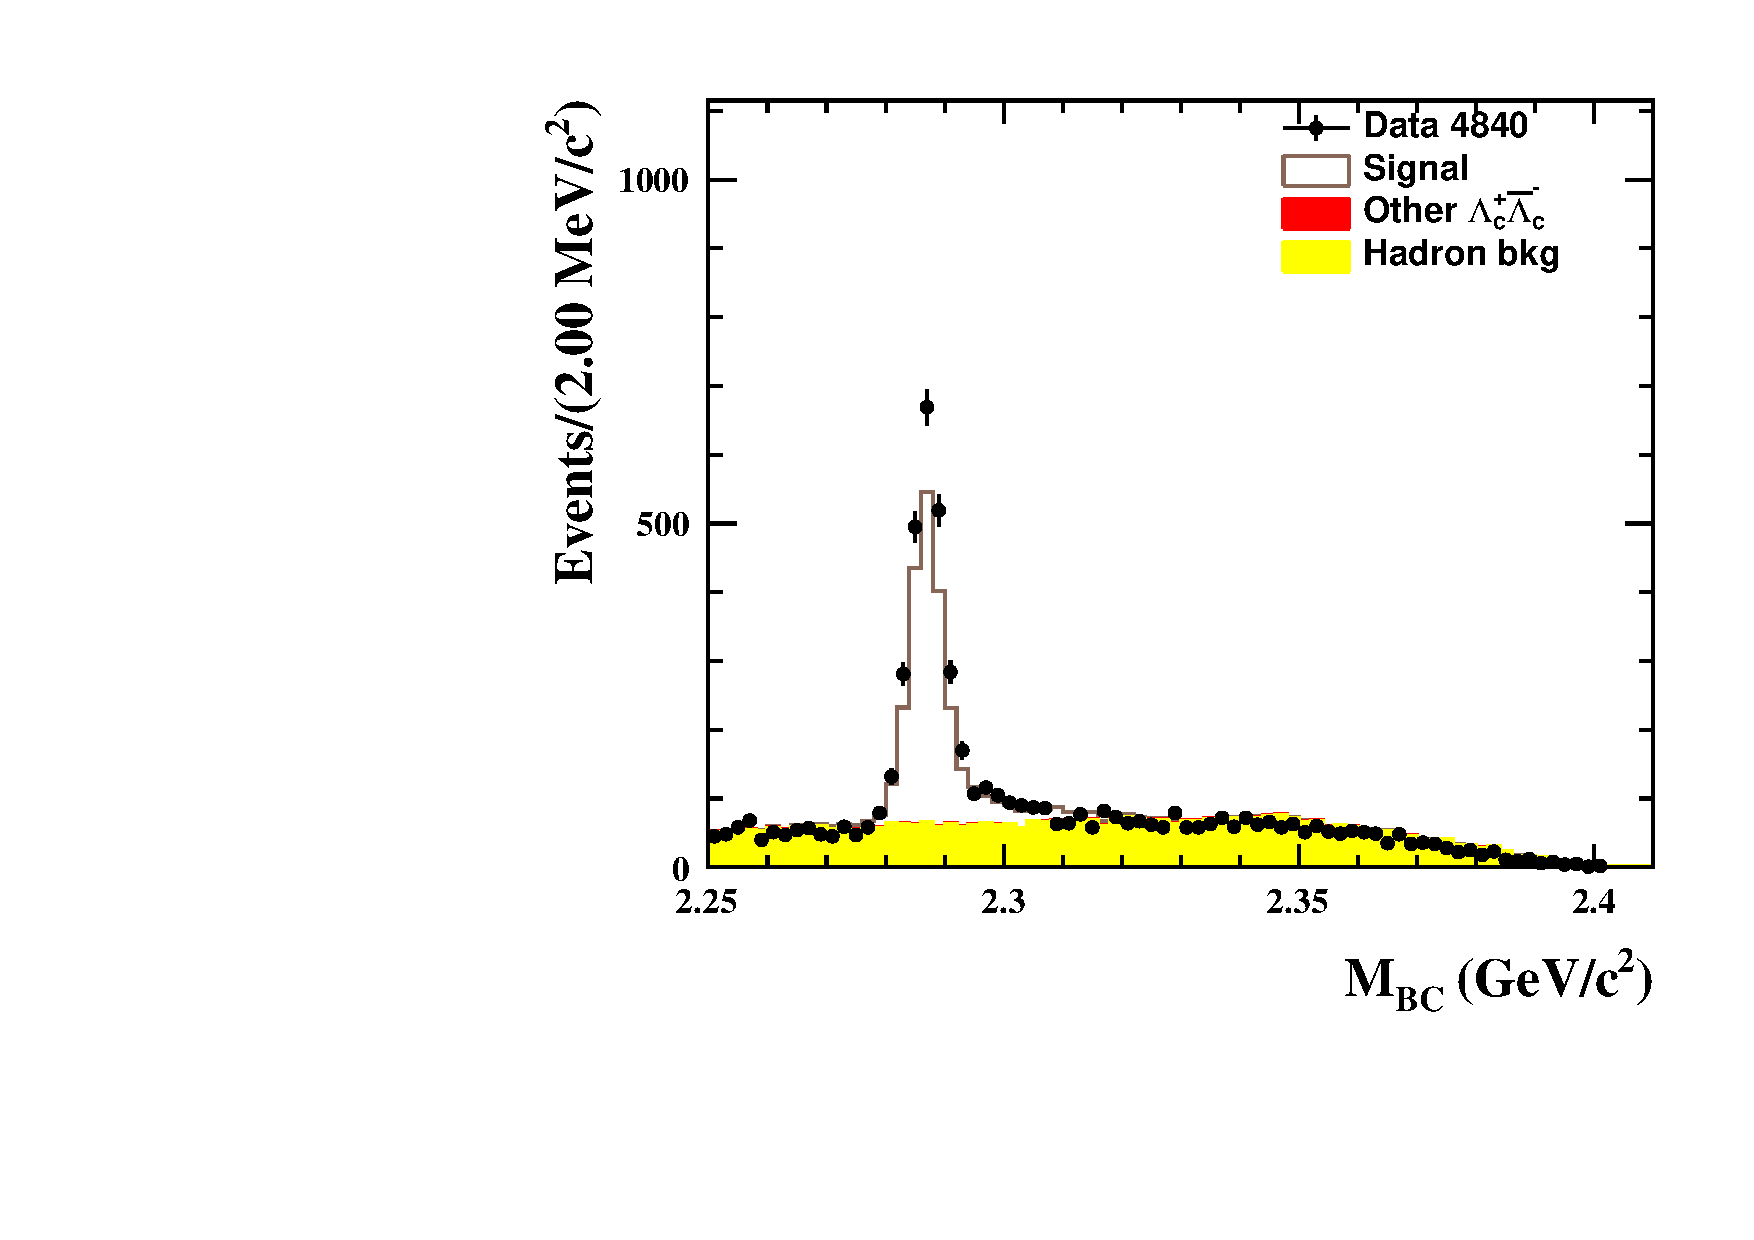
\includegraphics[width=0.24\textwidth]{figure/full_mbc/output_4840_mBC.pdf}
    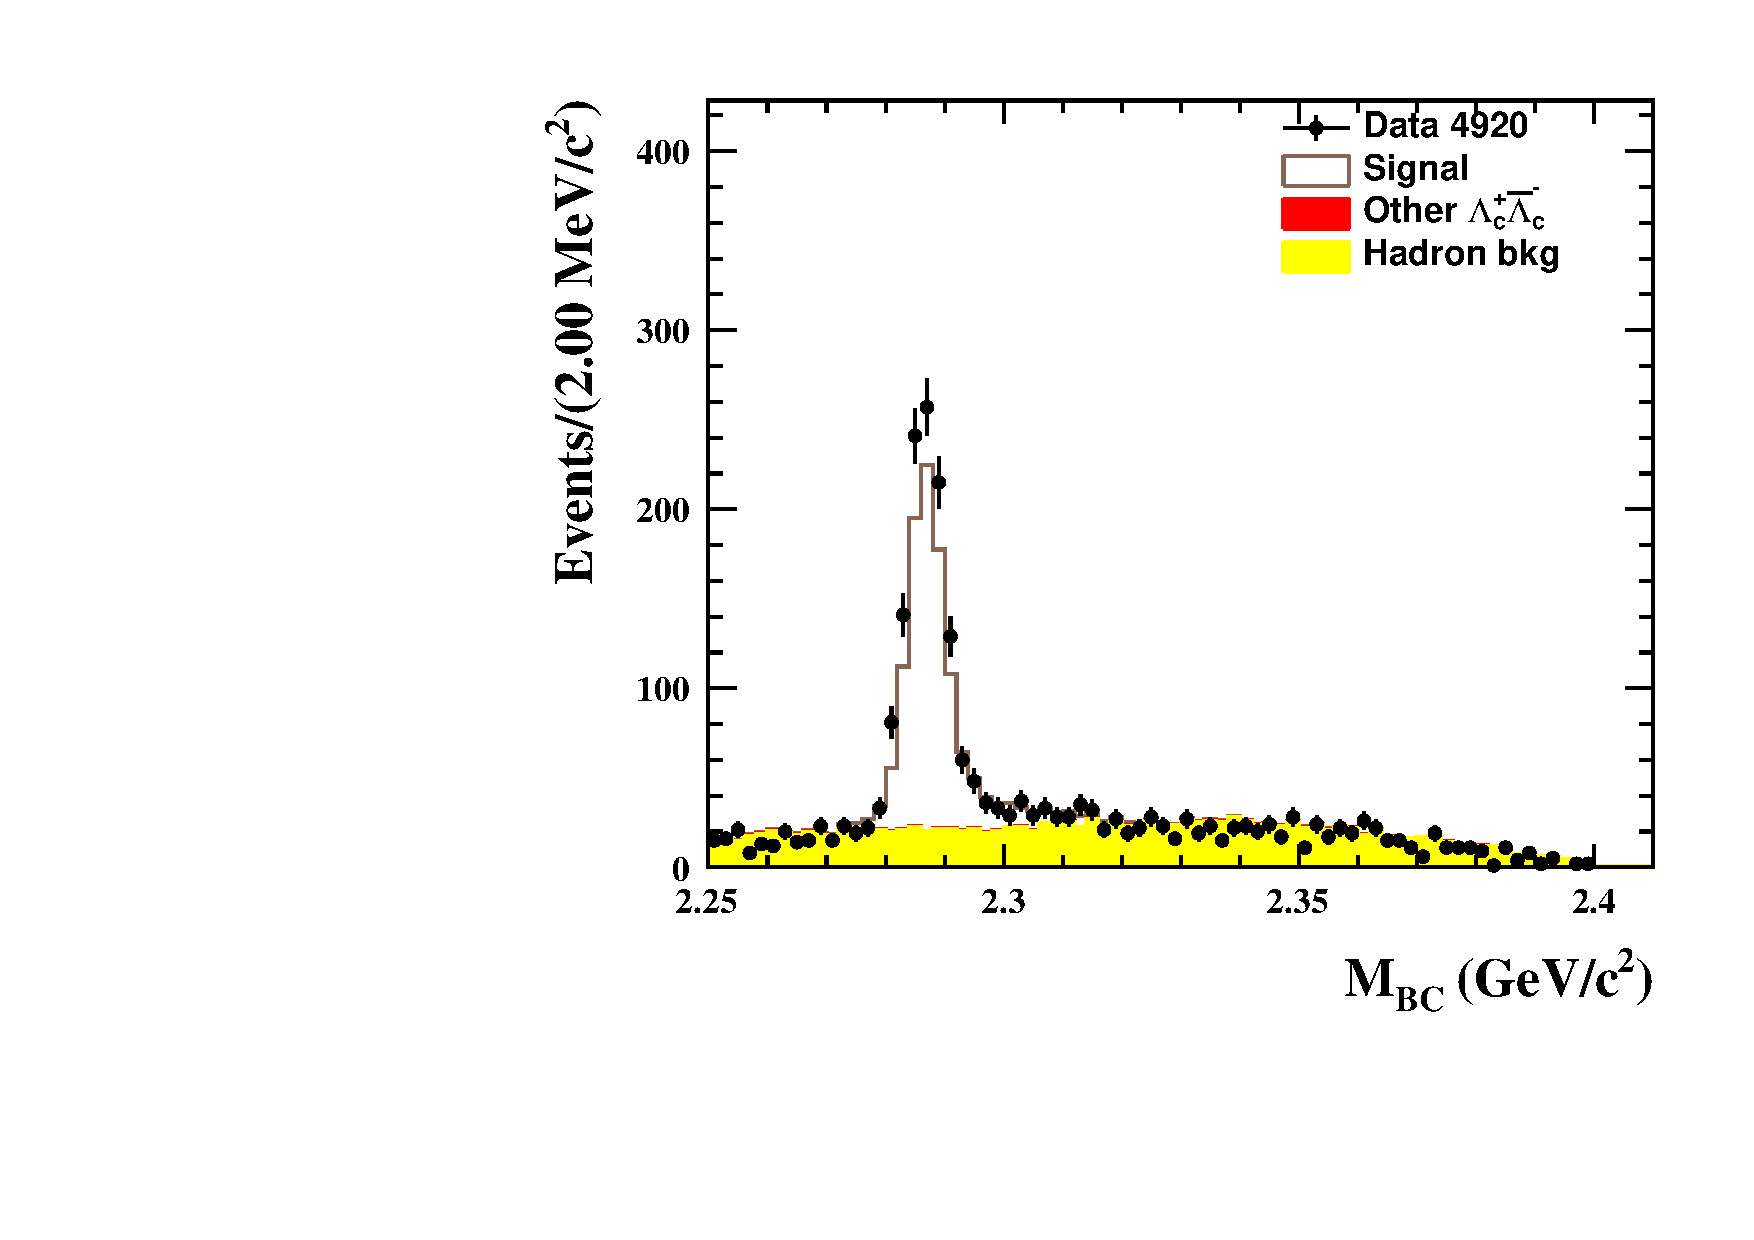
\includegraphics[width=0.24\textwidth]{figure/full_mbc/output_4914_mBC.pdf}
    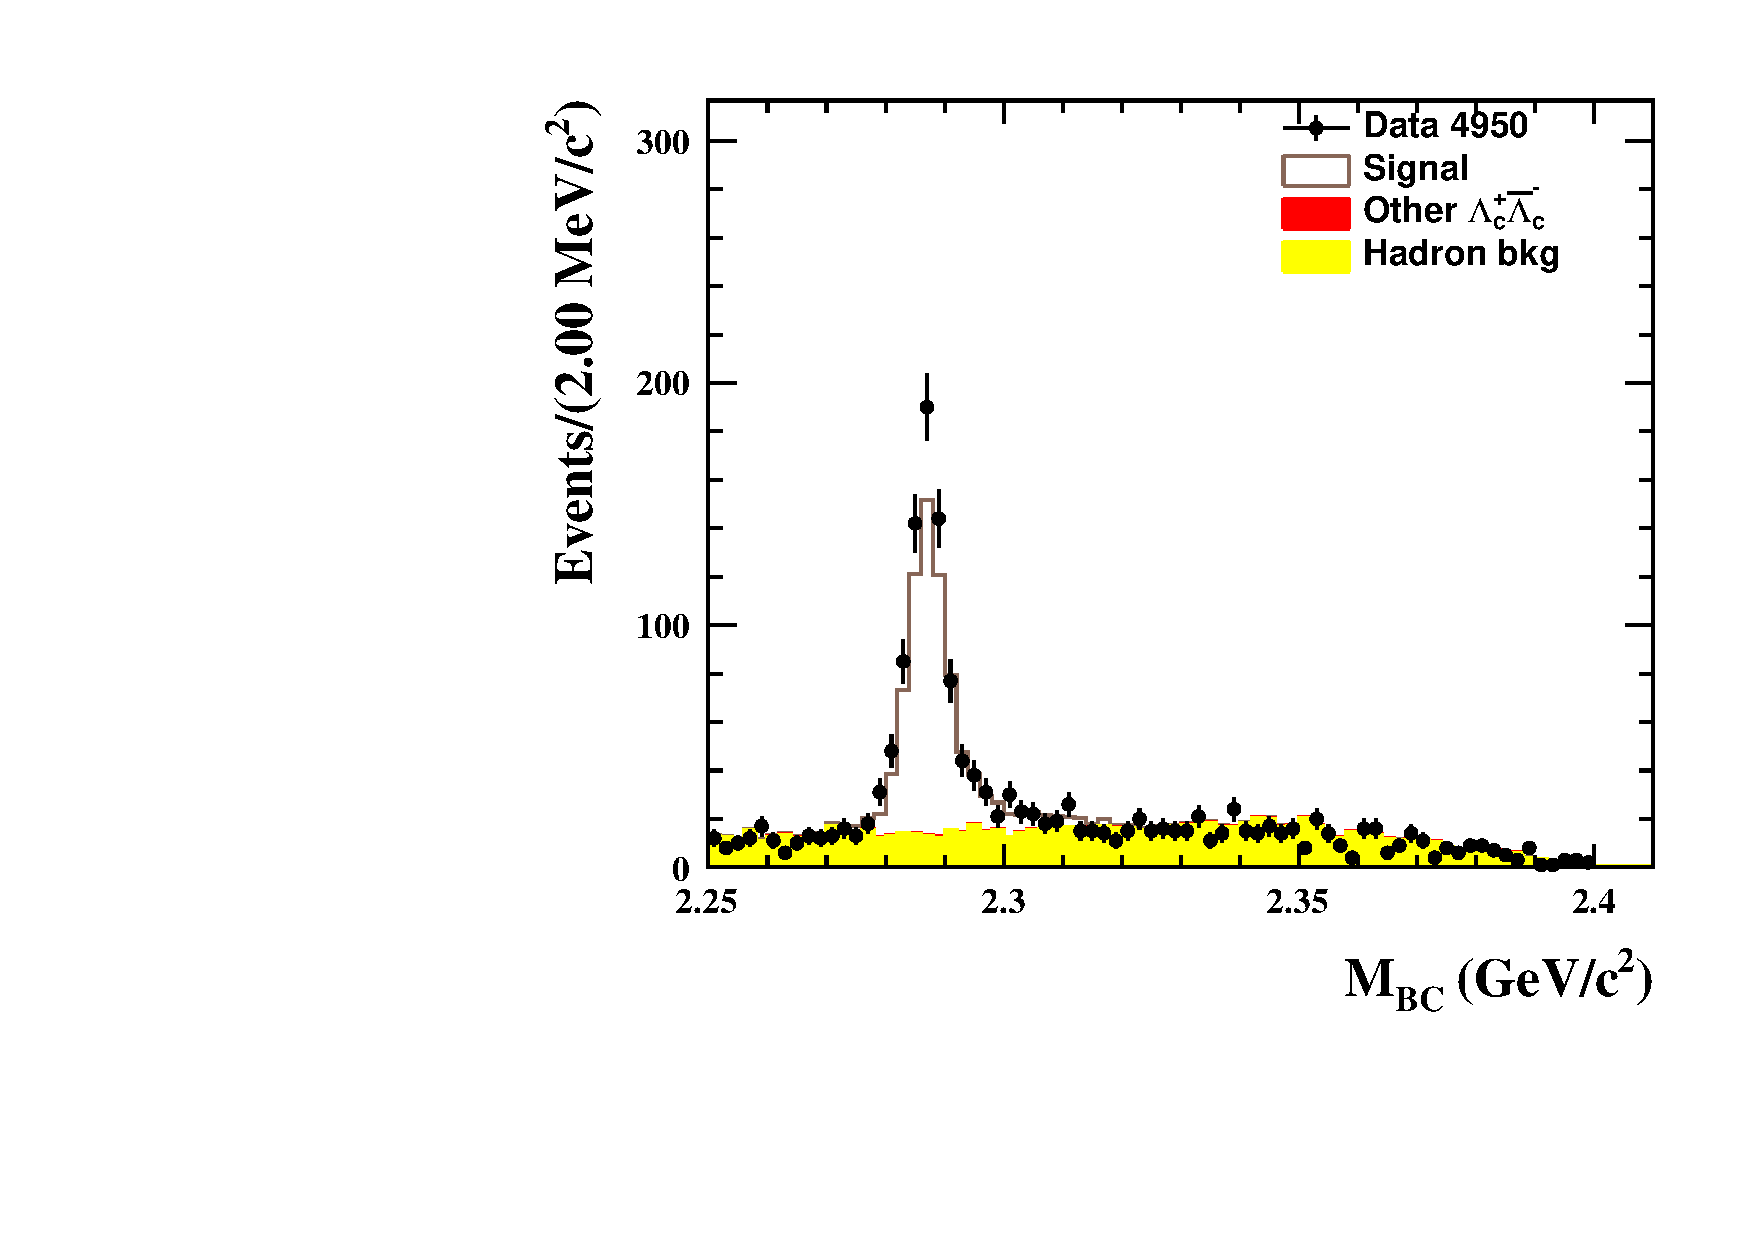
\includegraphics[width=0.24\textwidth]{figure/full_mbc/output_4946_mBC.pdf}
    \caption{Comparison of data and cocktail MC samples for each energy point. The cocktail MC samples are scaled to the integrated luminosity of data.}
\label{fig:full_mbc}
\end{figure}

\subsection{ST signal yields}
\label{sec:st_yields}

Extended unbinned maximum likelihood fits are conducted to extract the single-tag (ST) signal yields and purity from the $\mbc$ distributions across all energy points. In the fit, the signal shape is derived from the kernel-estimated non-parametric shape~\cite{Cranmer:2000du} of the phase space (PHSP) signal MC samples. To account for the discrepancies between data and MC simulations, a Gaussian function with adjustable parameters is convolved with the signal shape. For energy points below $\sqrt{s} = 4.740\gev/c^2$, the background shape is described by the ARGUS~\cite{Djouadi:1989hh} function, defined as follows:
\begin{equation}
P_{\rm bkg}(\mbc,E_0,c,p) = \mbc \left(1 - \left(\frac{\mbc}{E_0}\right)^2 \right)^p \times e^{c \left(1-\frac{\mbc}{E_0}\right)^2},
\end{equation}
where $E_0$ represents the endpoint of $\mbc$ and is fixed at the beam energy. The parameters $p$ and $c$ correspond to the power parameter and the scale factor, respectively. The default value for $p$ is set to 0.5 and is held fixed, while $c$ is allowed to vary in the fit. For the remaining points, the $\mbc$ distributions have cutoff points at approximately 2.4$\gev/c^2$ due to %the $\dE$ requirements. 
an additional cut $|M(pK^-\pi^+) - m_{\lcp}| < 0.085\gev/c^2$, where $M(pK^-\pi^+)$ denotes the reconstructed invariant mass of $pK^-\pi^+$ and $m_{\lcp}$ represents the nominal mass value of $\lcp$ in PDG.
The fit region is narrowed to (2.25, 2.34)$\gev/c^2$ and a second-order Chebyshev polynomial function is employed to model the background shape. The overall probability density function (PDF) is parameterized as the summation of signal and background components. The $\mbc$ signal and sideband regions are determined to be (2.282, 2.291) and (2.25, 2.27) $\gev/c^2$, respectively. The fit results are visualized in Figure~\ref{fig:fit_mbc}. Within the $\mbc$ signal region, the background fraction ($f_{\rm bkg}$) is determined using the equation $f_{\rm bkg} = n_{\rm bkg}/(n_{\rm sig} + n_{\rm bkg})$, where $n_{\rm sig}$ and $n_{\rm bkg}$ denote the event yields for the signal and background components, respectively. 
The uncertainties associated with the background fractions are computed using the formula:
\begin{equation}
    \sigma_{\rm bkg} = \sqrt{(1-2*f_{\rm bkg})n_{\rm bkg} + f_{\rm bkg}^2(n_{\rm sig} + n_{\rm bkg})}.
\end{equation}
The signal purities are determined as $f_{\rm sig} = 1 - f_{\rm bkg}$, and are generally larger than 90\% to ensure a reliable amplitude analysis.
The fit results within $\mbc$ signal region are summarized in Table~\ref{tab:fit_mbc_results}.

\begin{figure}\centering
    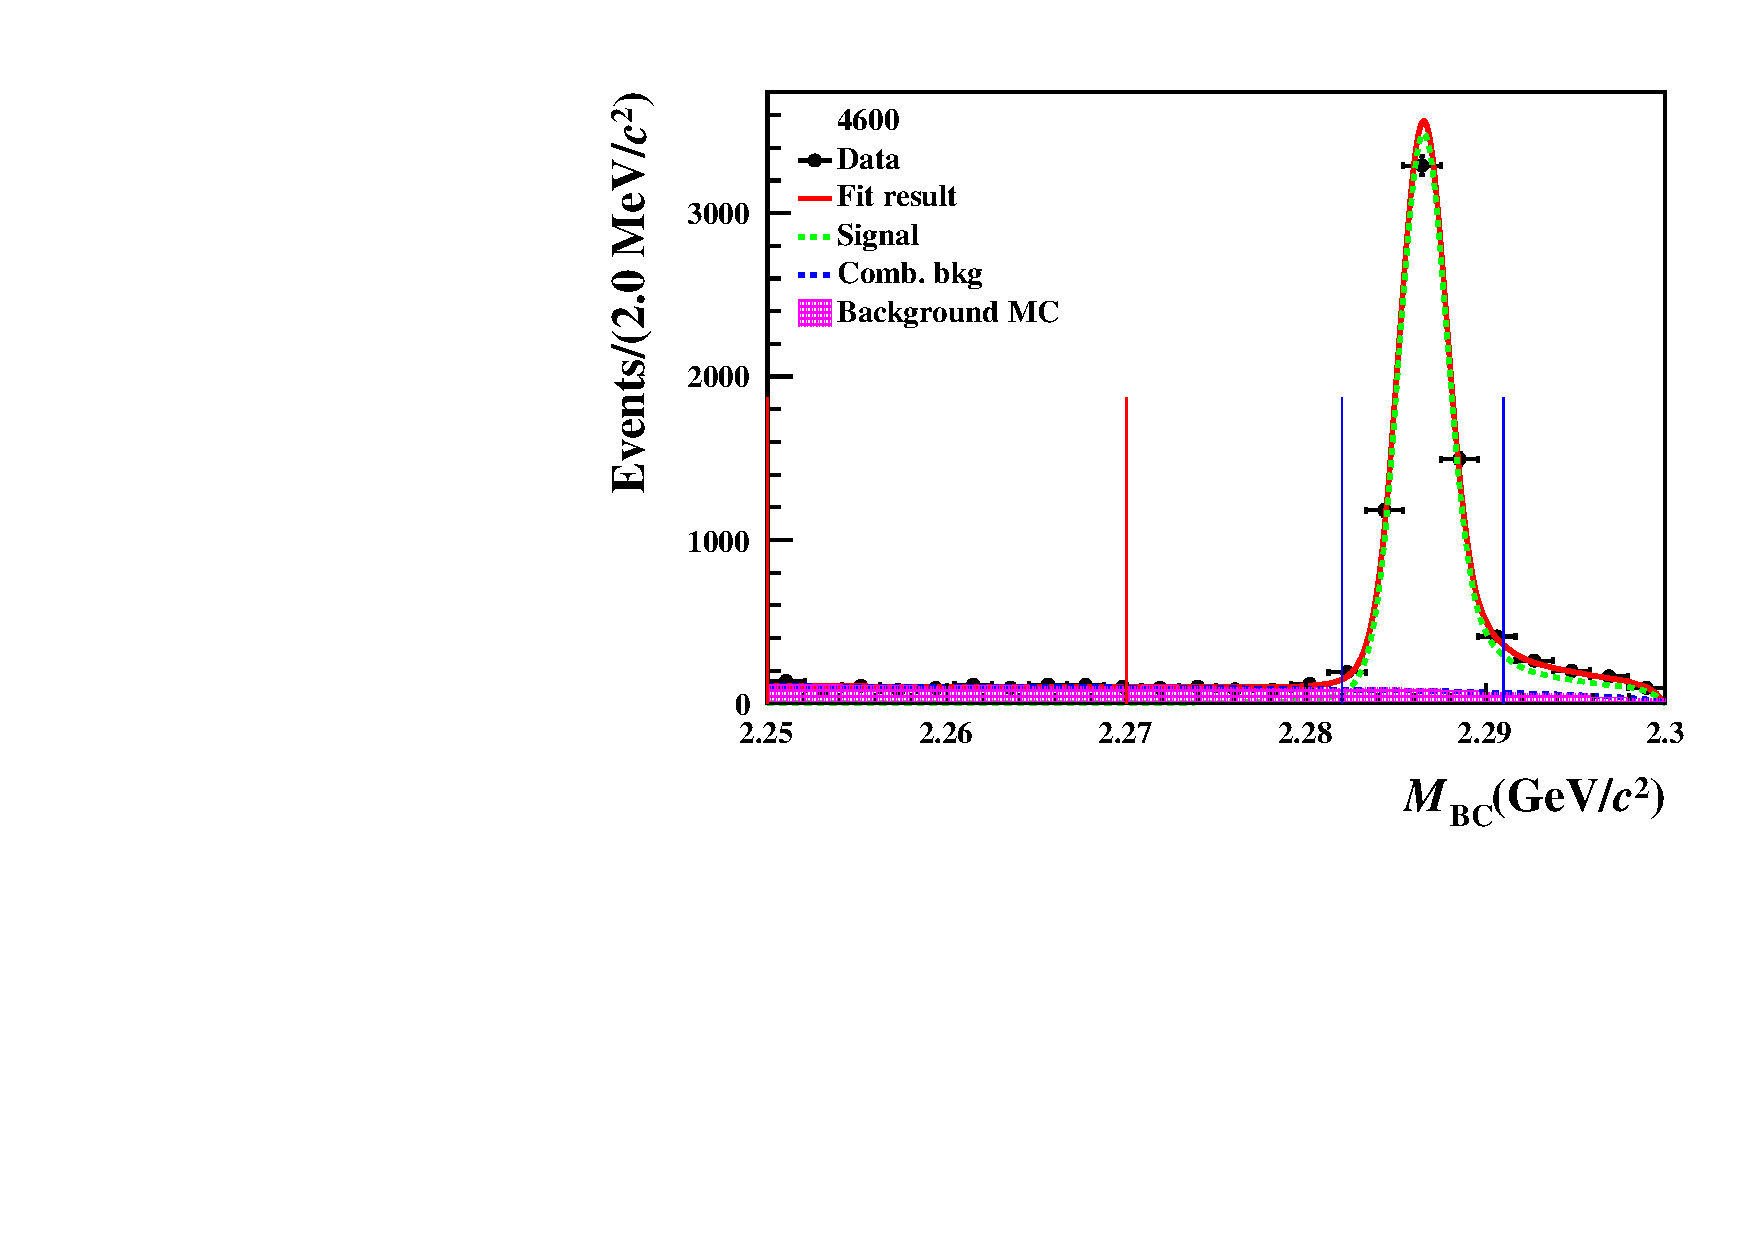
\includegraphics[width=0.24\textwidth]{figure/fit_mbc/fit_mBC_data4600.pdf}
    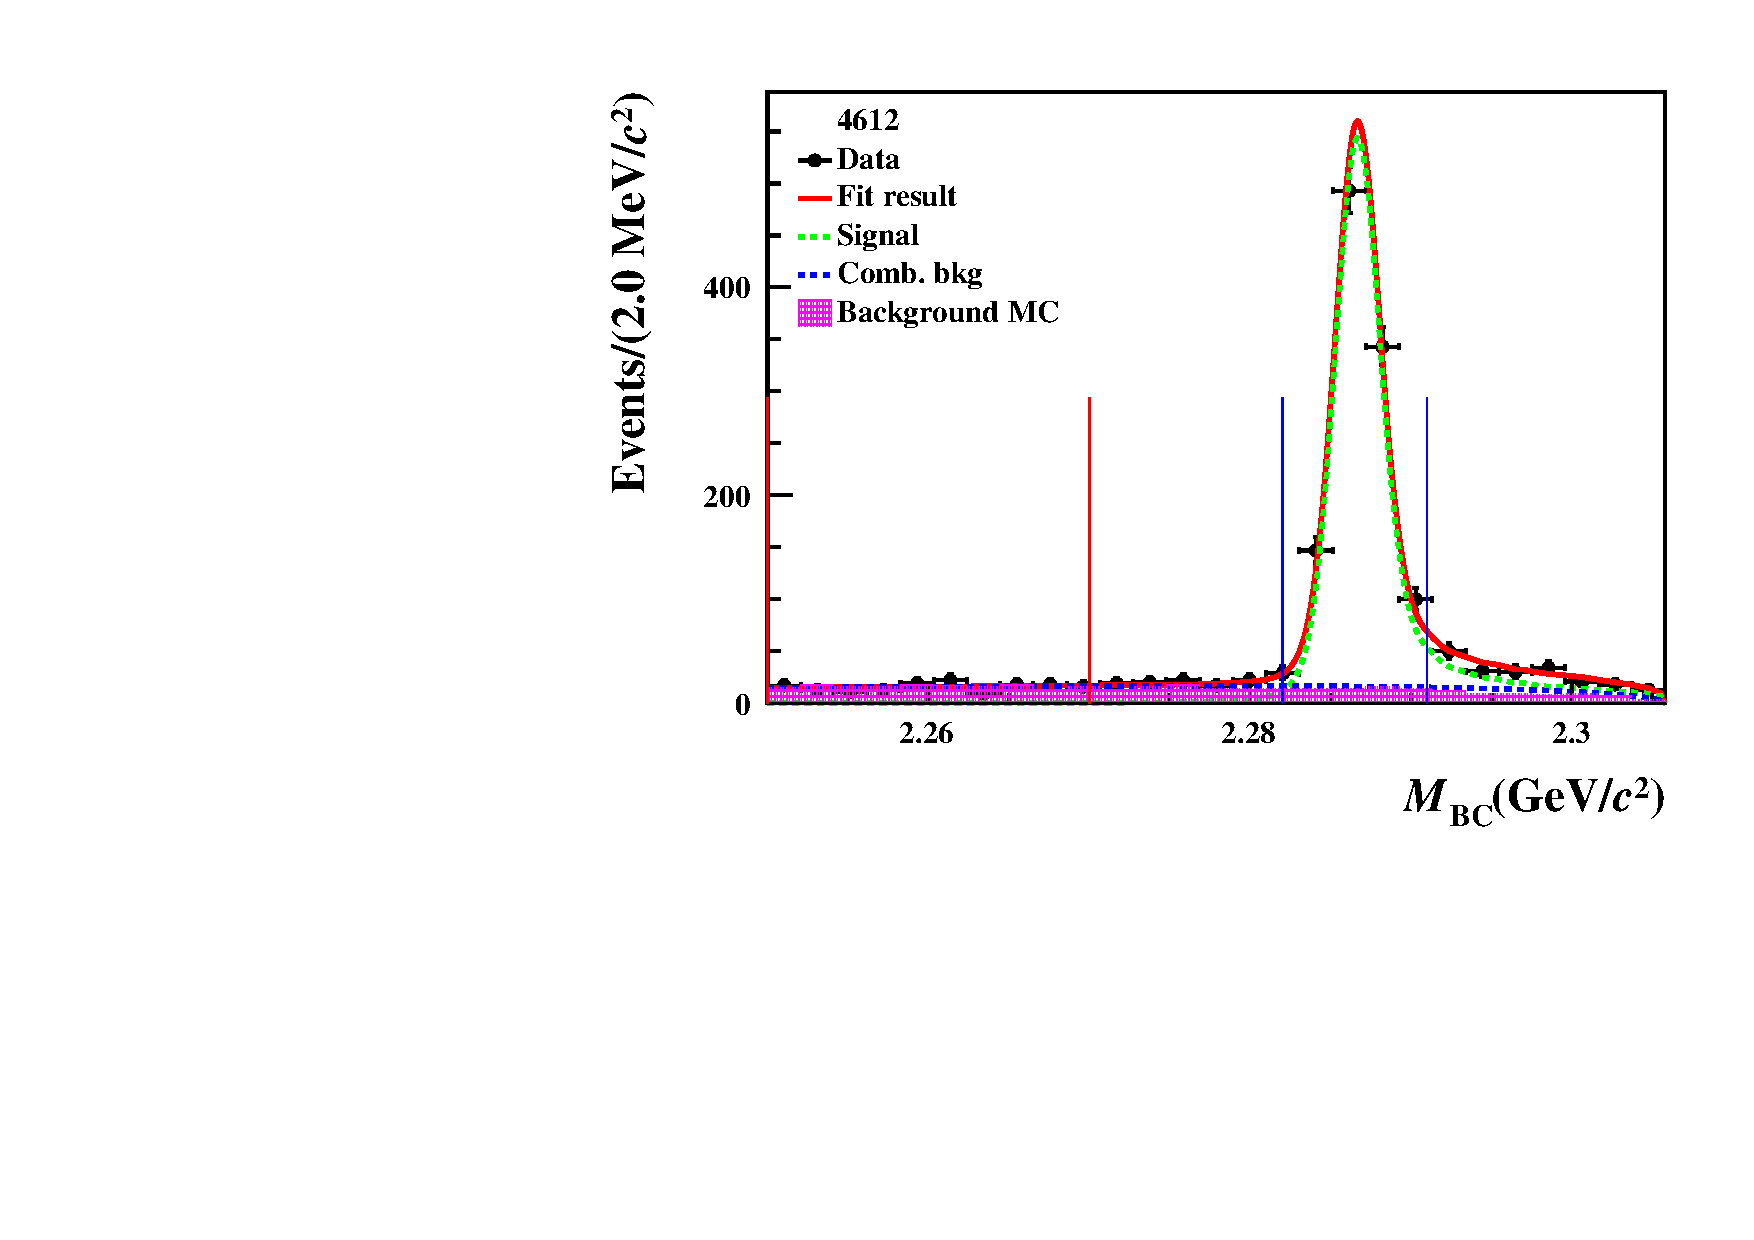
\includegraphics[width=0.24\textwidth]{figure/fit_mbc/fit_mBC_data4612.pdf}
    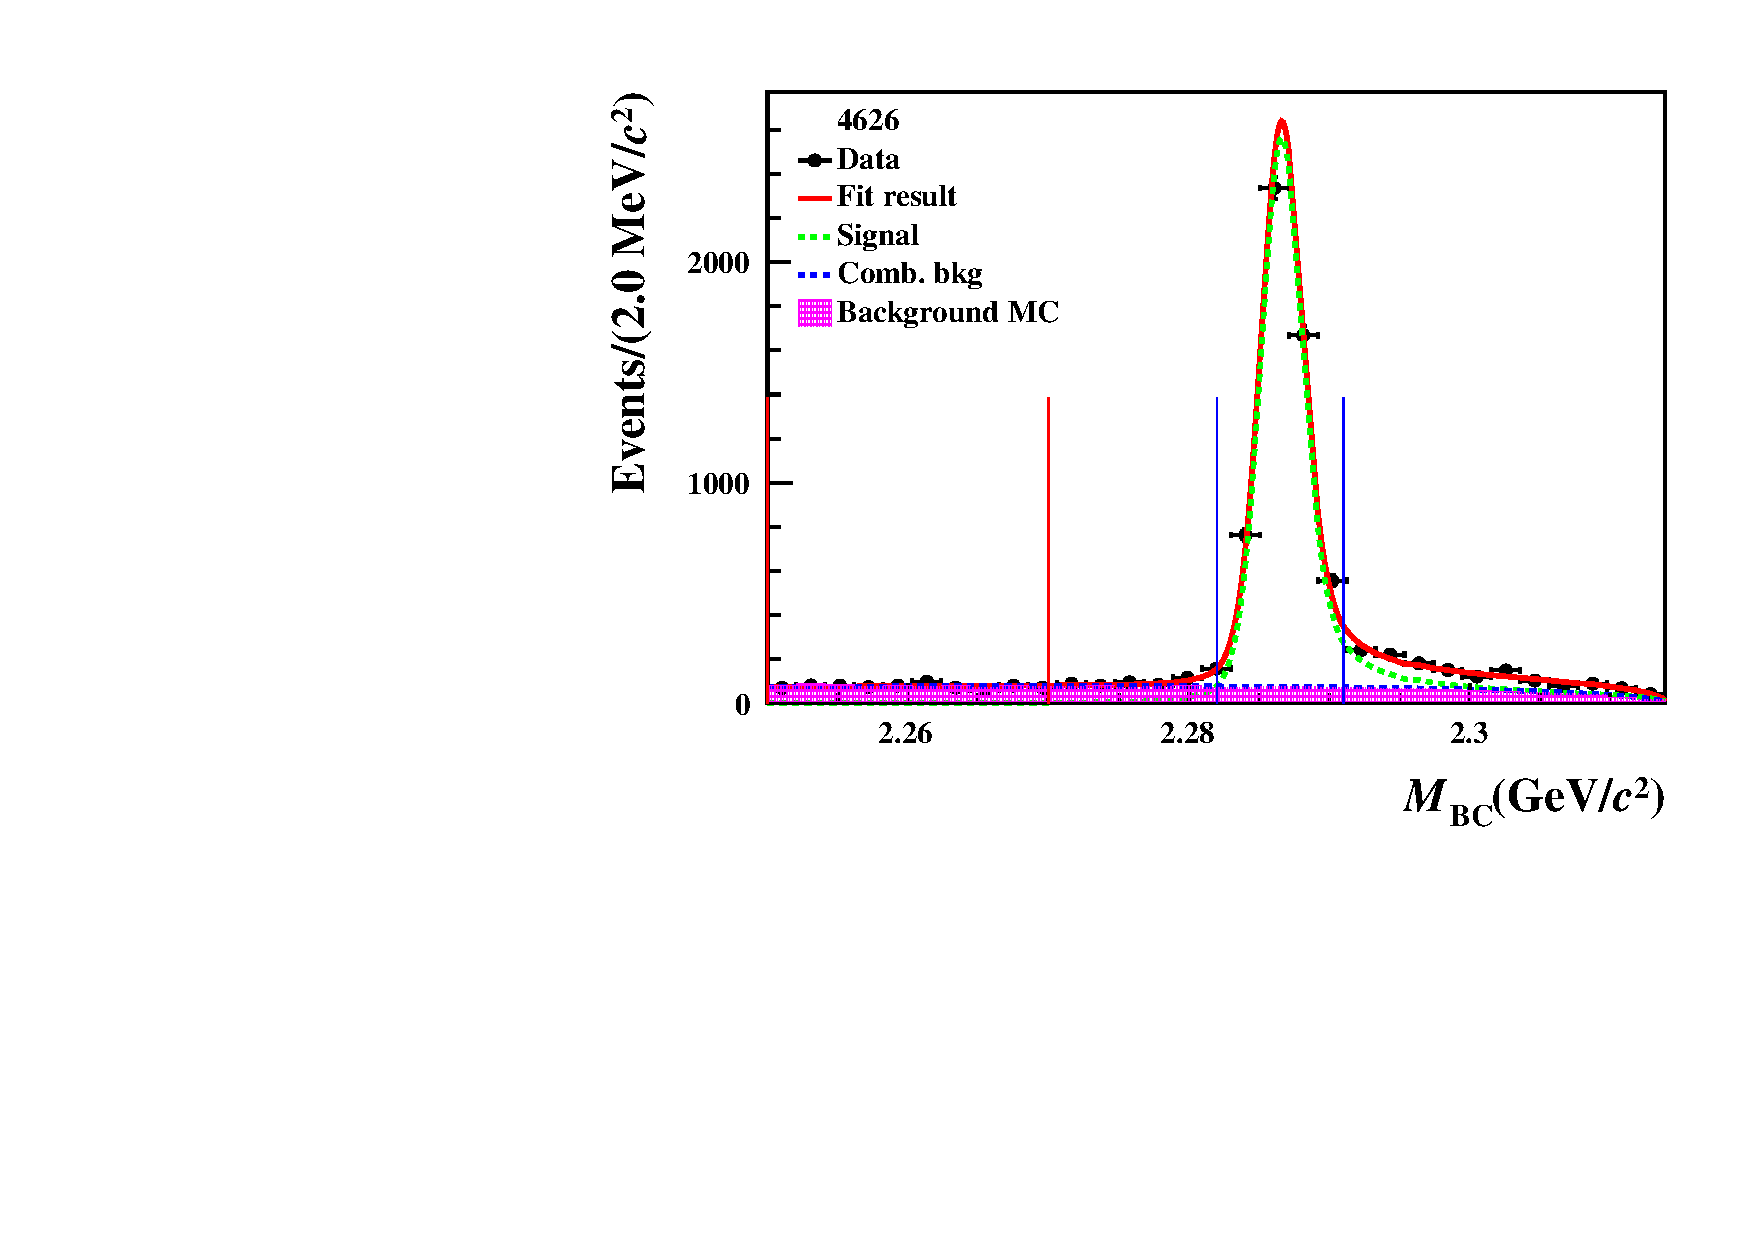
\includegraphics[width=0.24\textwidth]{figure/fit_mbc/fit_mBC_data4626.pdf}
    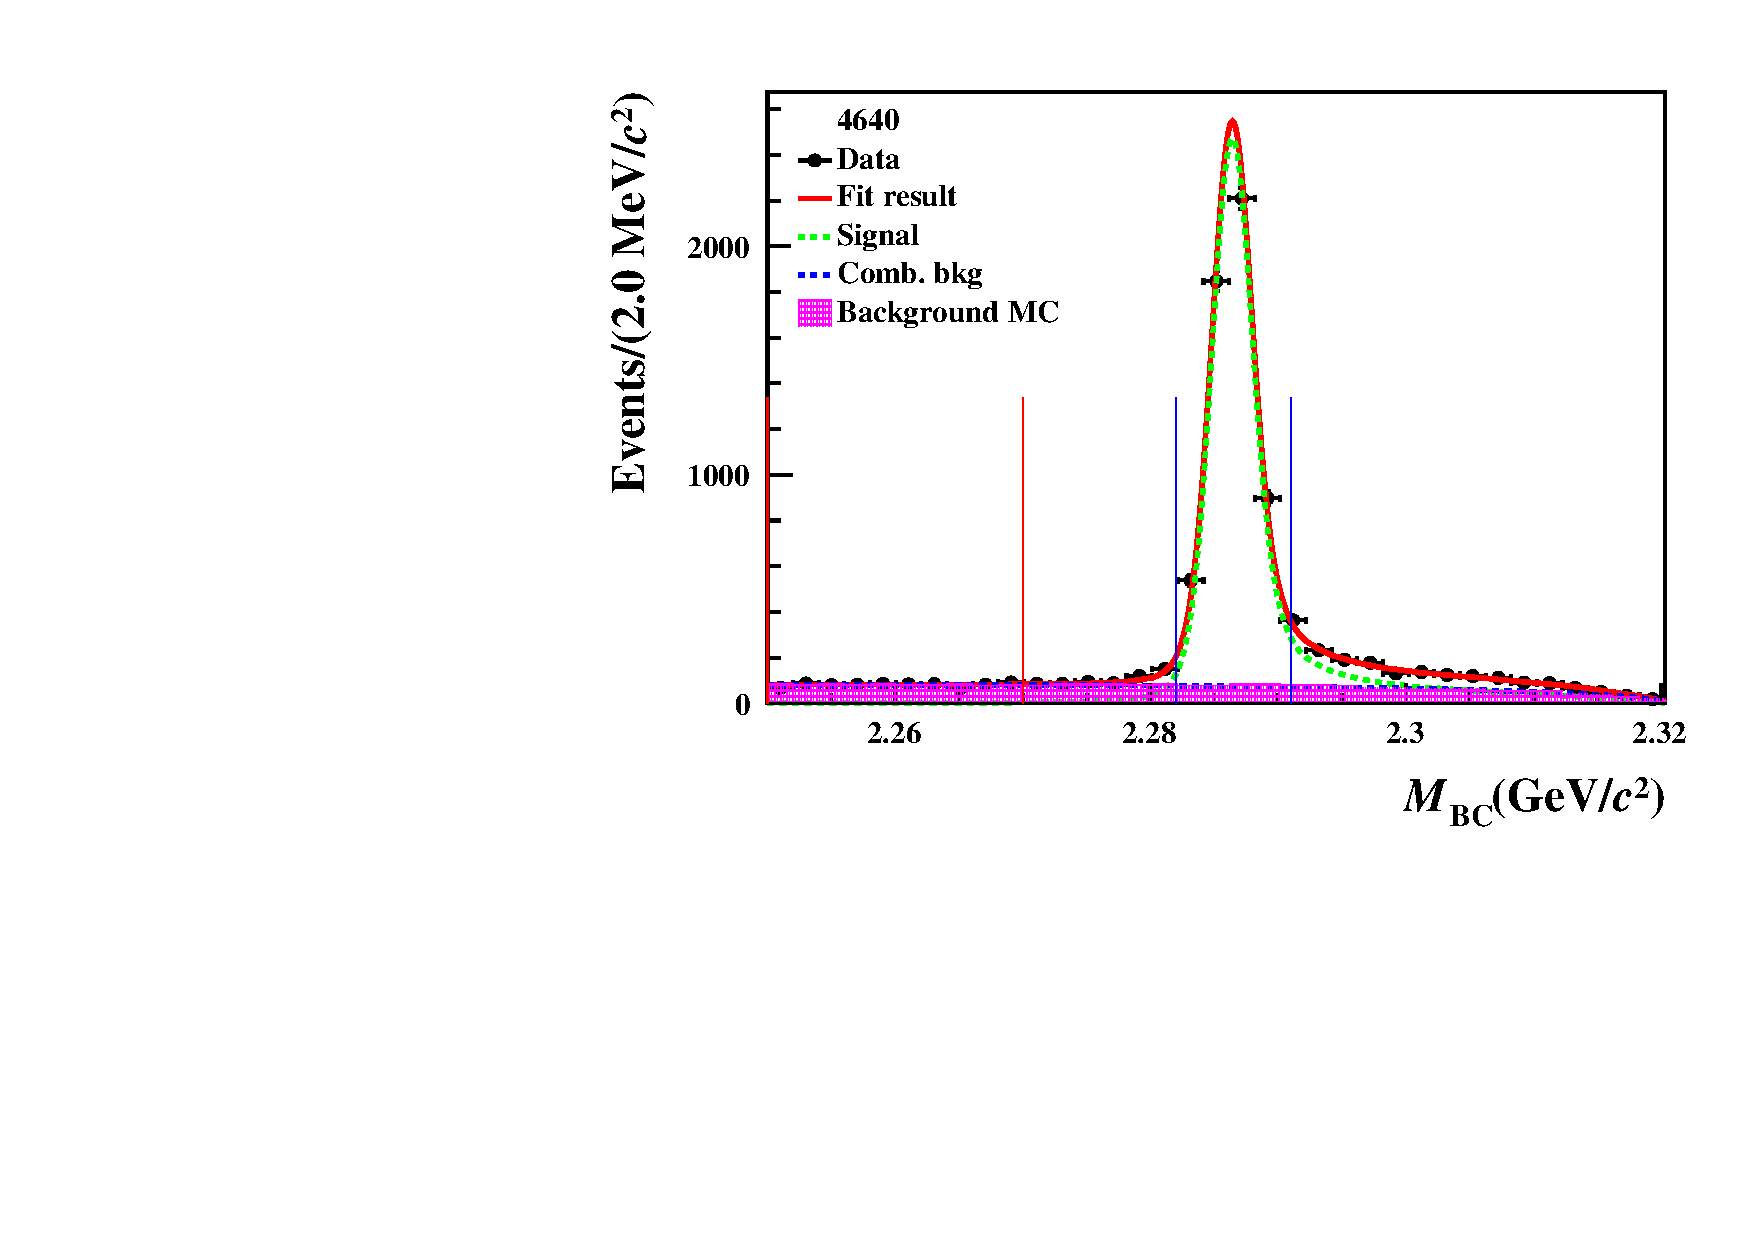
\includegraphics[width=0.24\textwidth]{figure/fit_mbc/fit_mBC_data4640.pdf}
    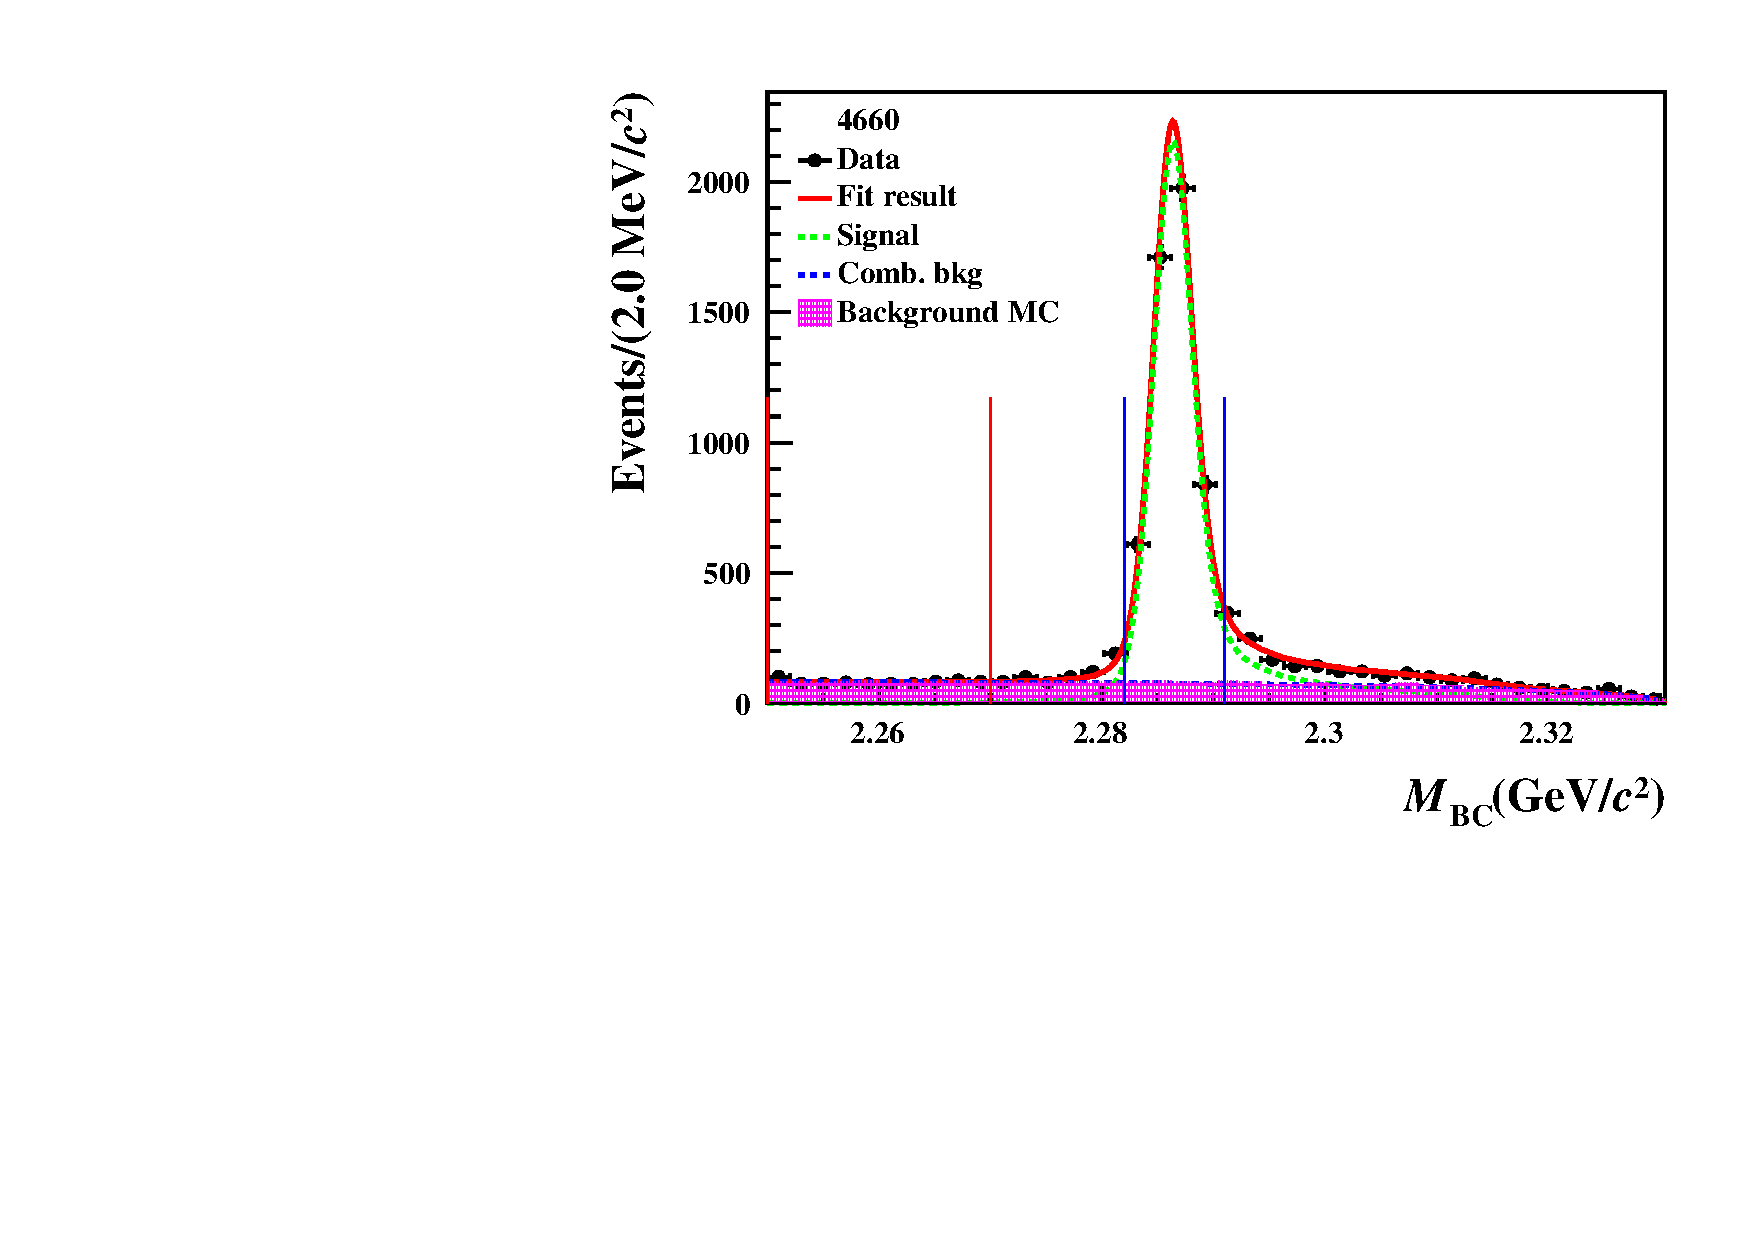
\includegraphics[width=0.24\textwidth]{figure/fit_mbc/fit_mBC_data4660.pdf}
    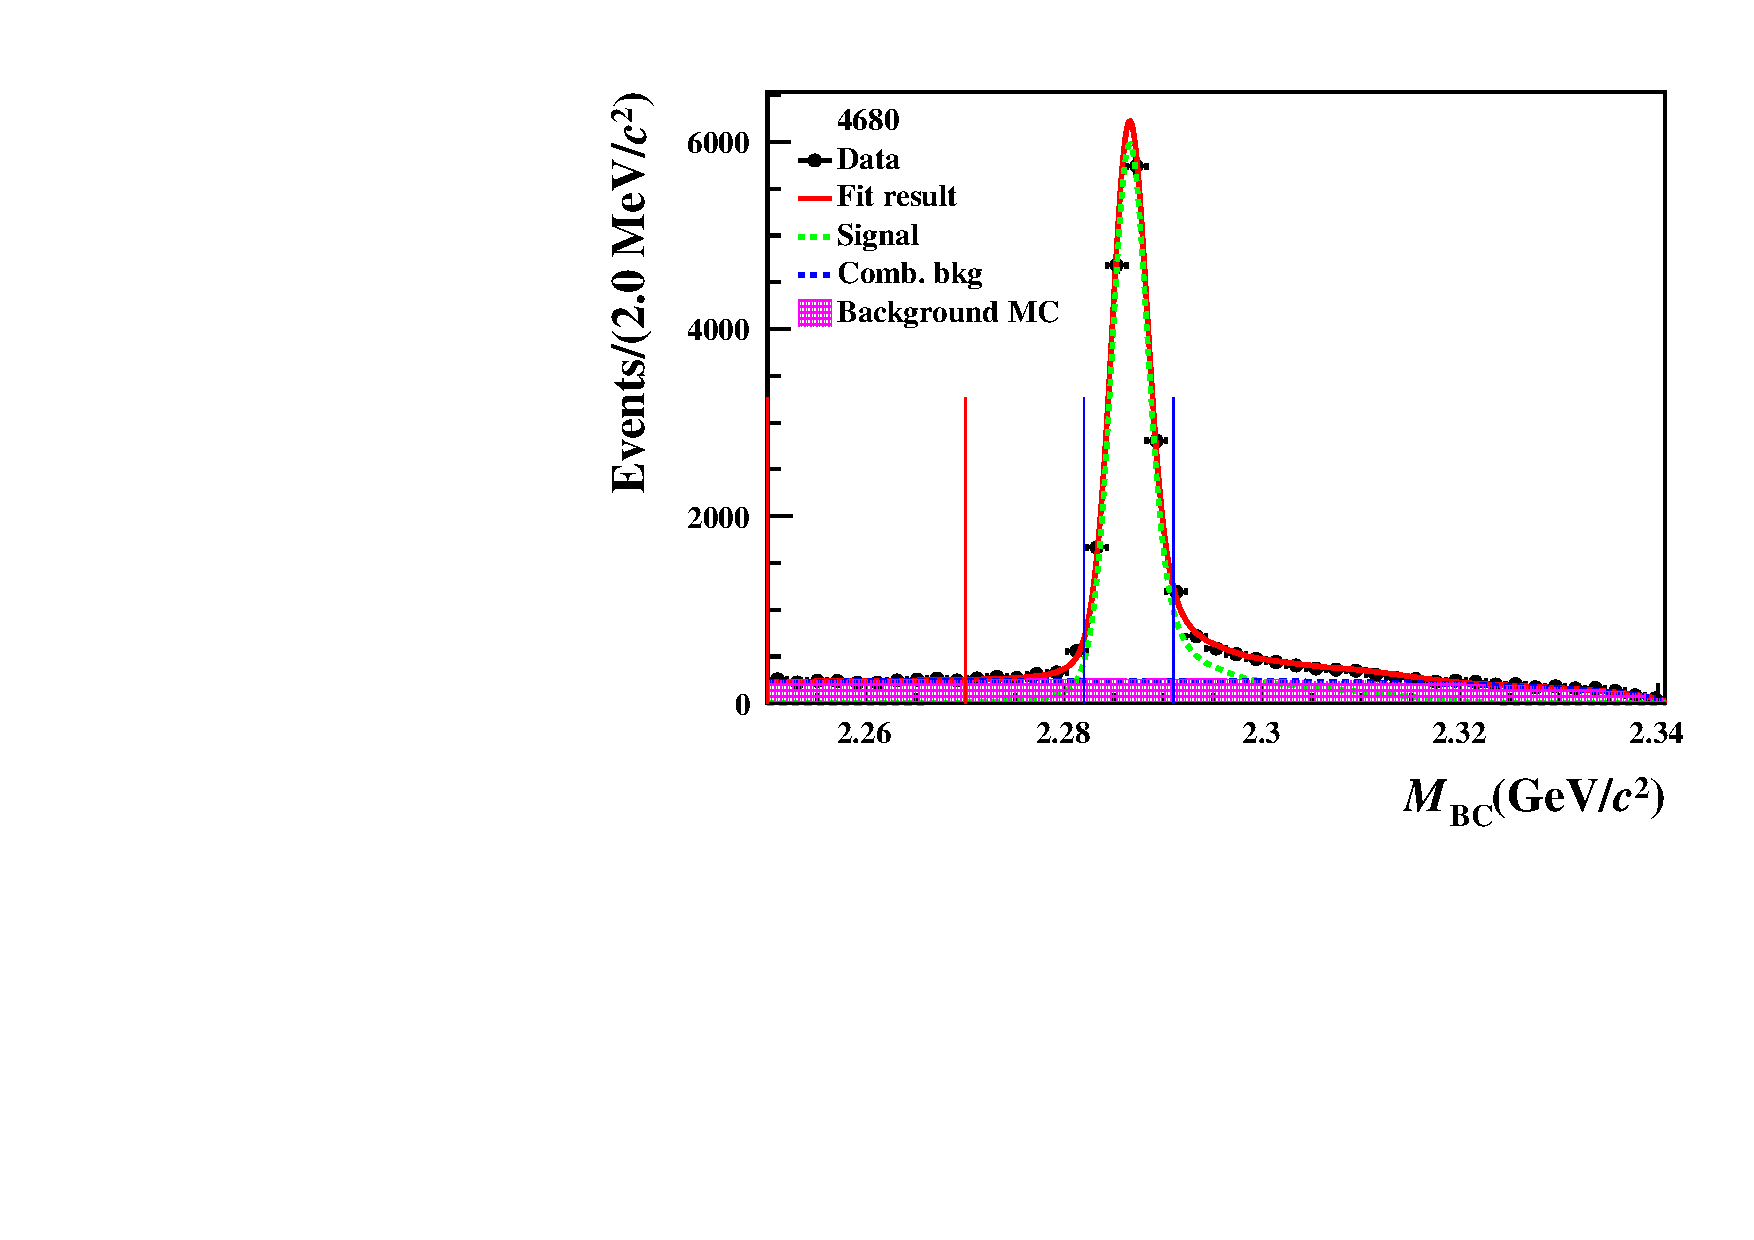
\includegraphics[width=0.24\textwidth]{figure/fit_mbc/fit_mBC_data4680.pdf}
    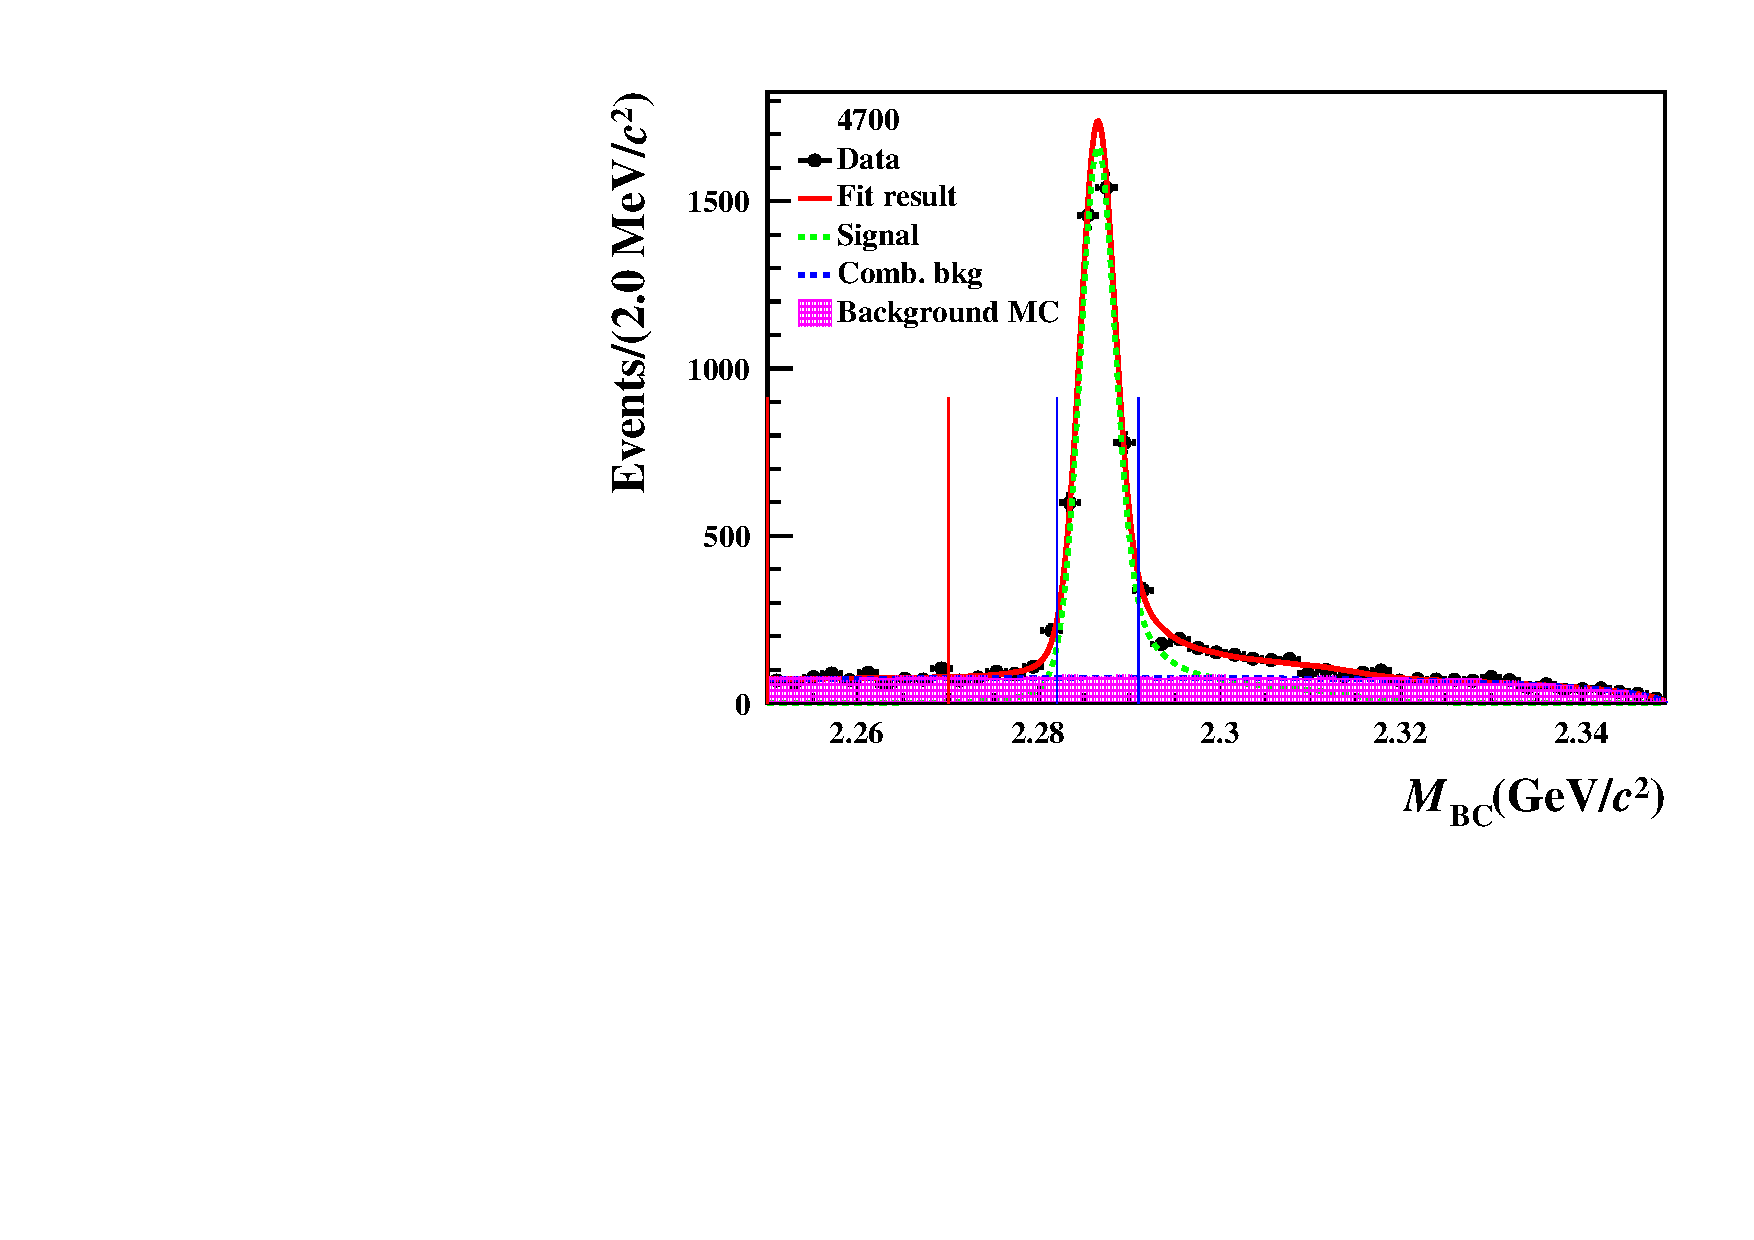
\includegraphics[width=0.24\textwidth]{figure/fit_mbc/fit_mBC_data4700.pdf}
    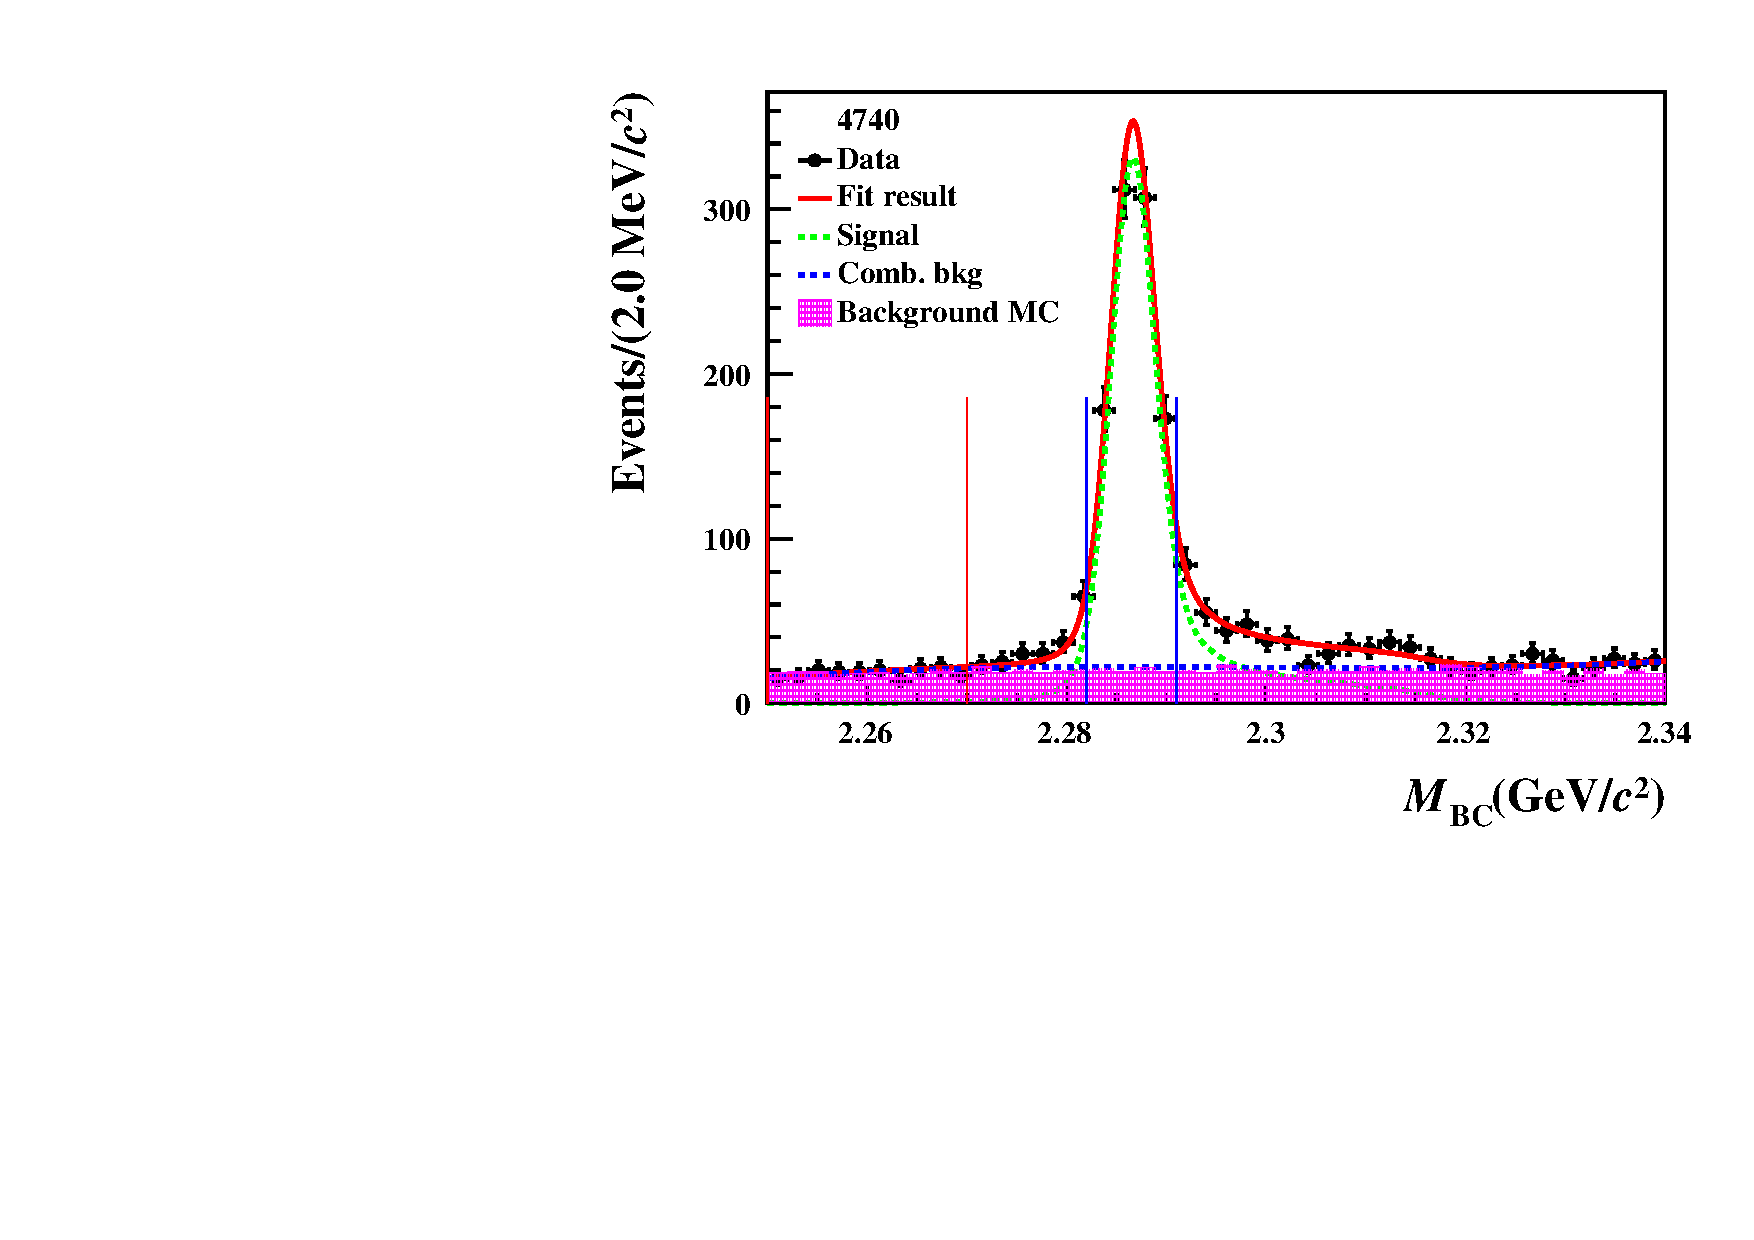
\includegraphics[width=0.24\textwidth]{figure/fit_mbc/fit_mBC_data4740.pdf}
    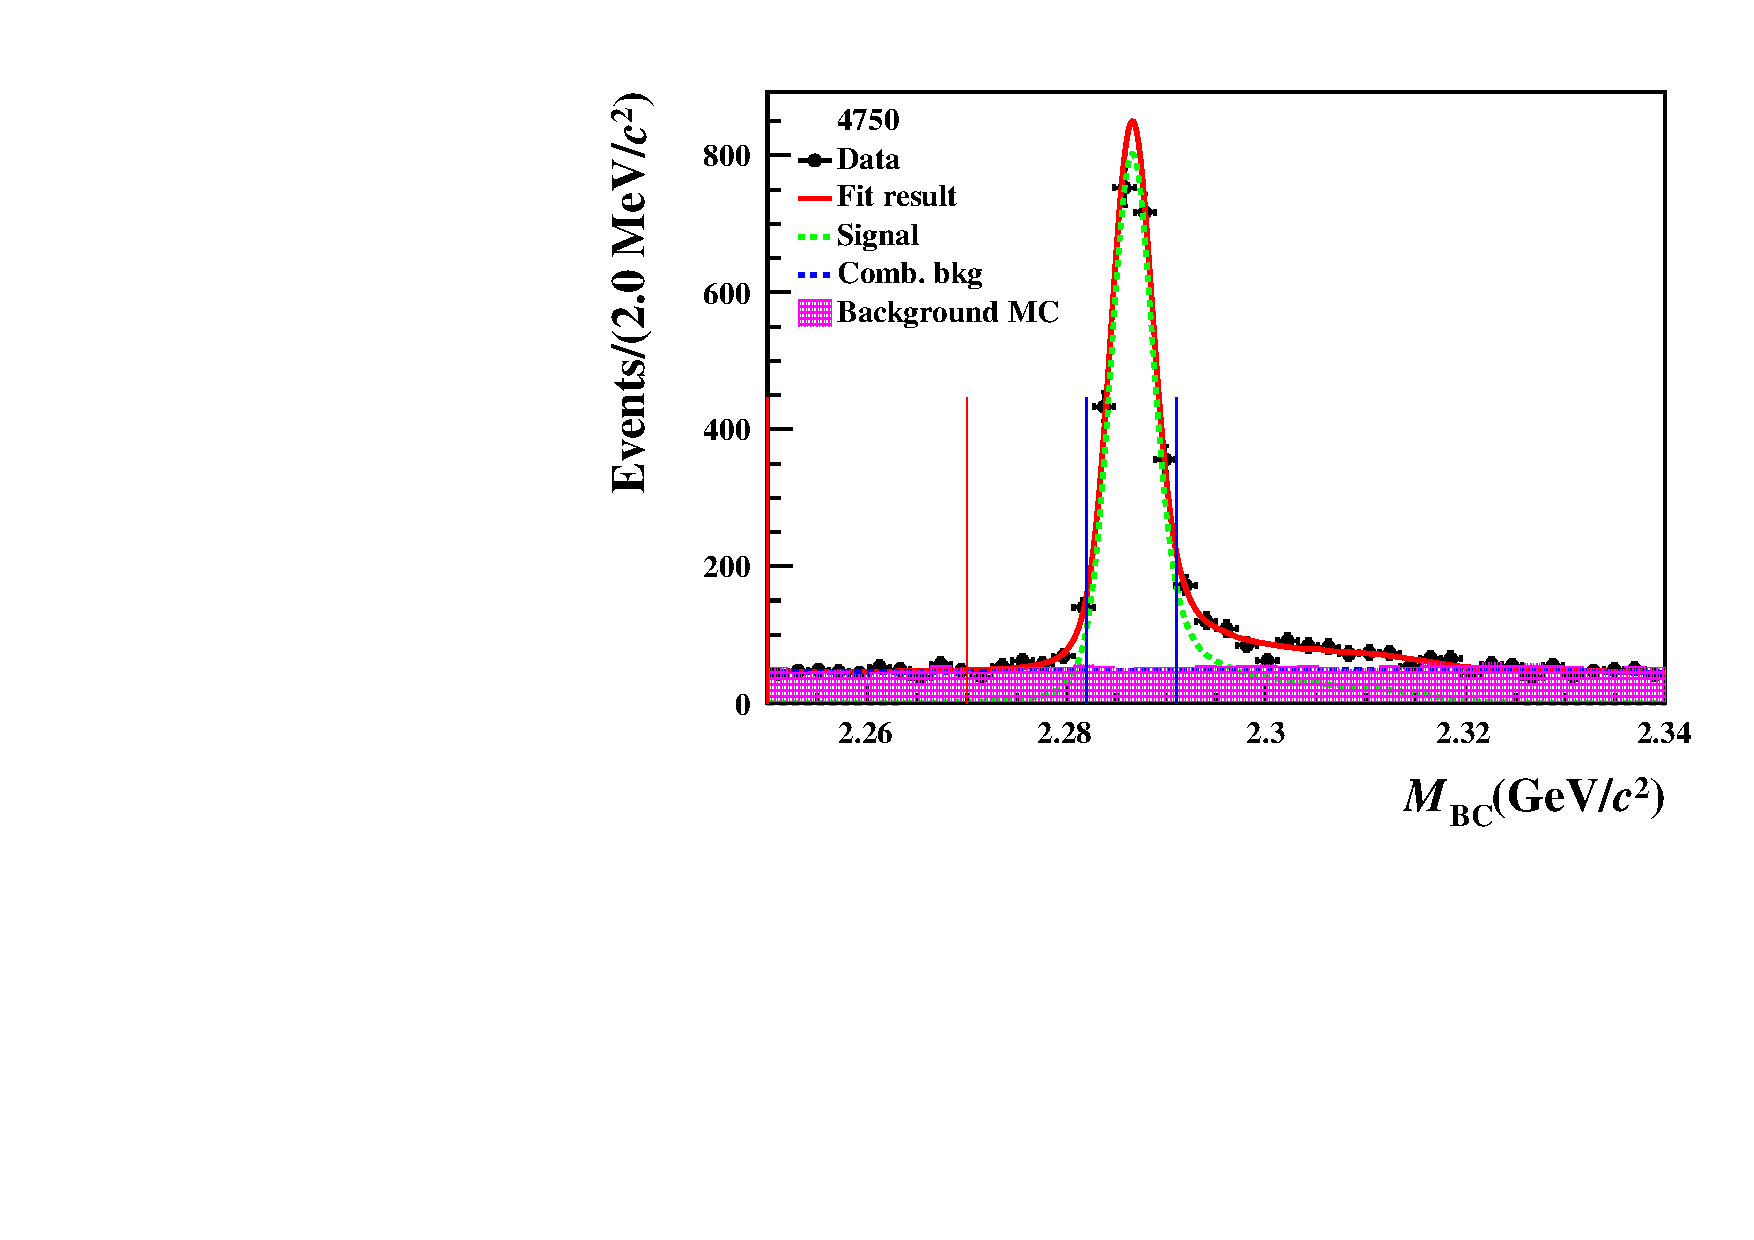
\includegraphics[width=0.24\textwidth]{figure/fit_mbc/fit_mBC_data4750.pdf}
    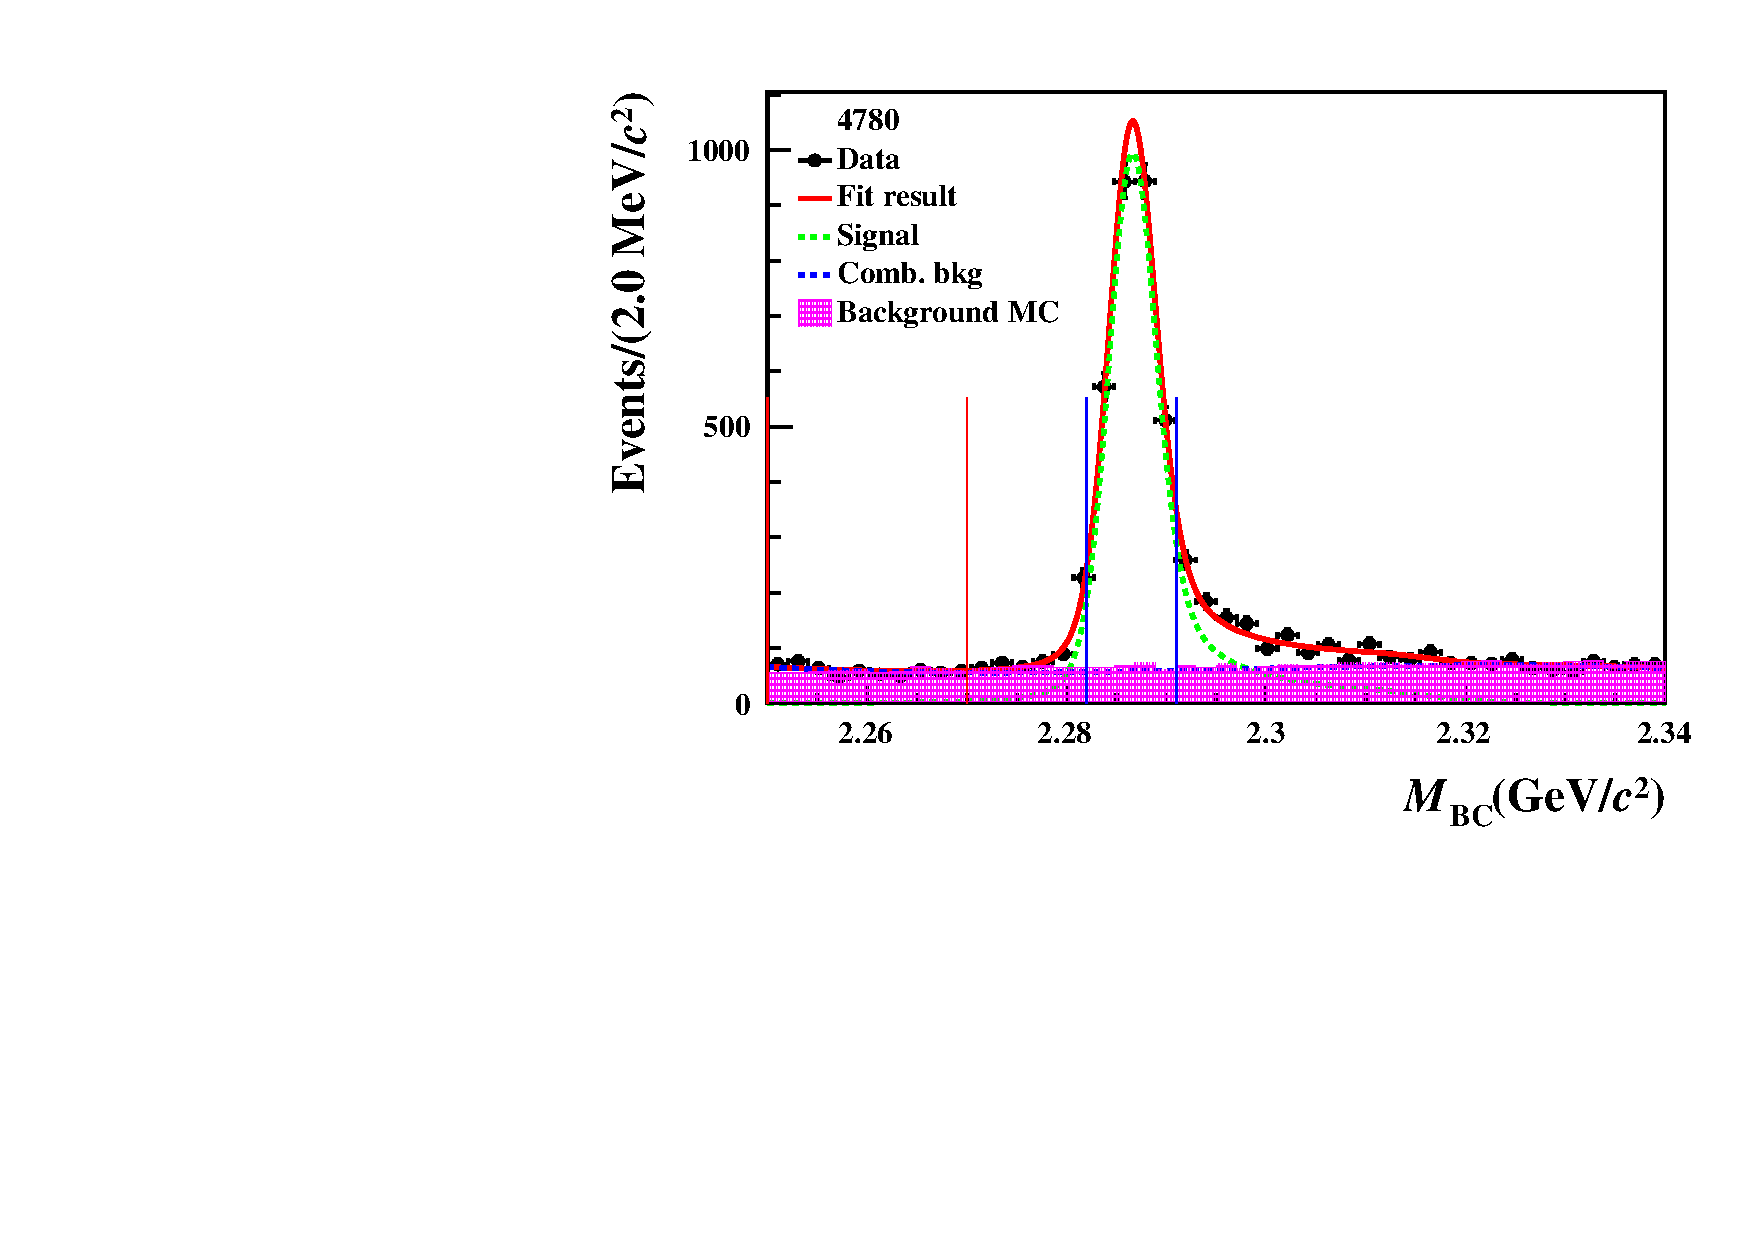
\includegraphics[width=0.24\textwidth]{figure/fit_mbc/fit_mBC_data4780.pdf}
    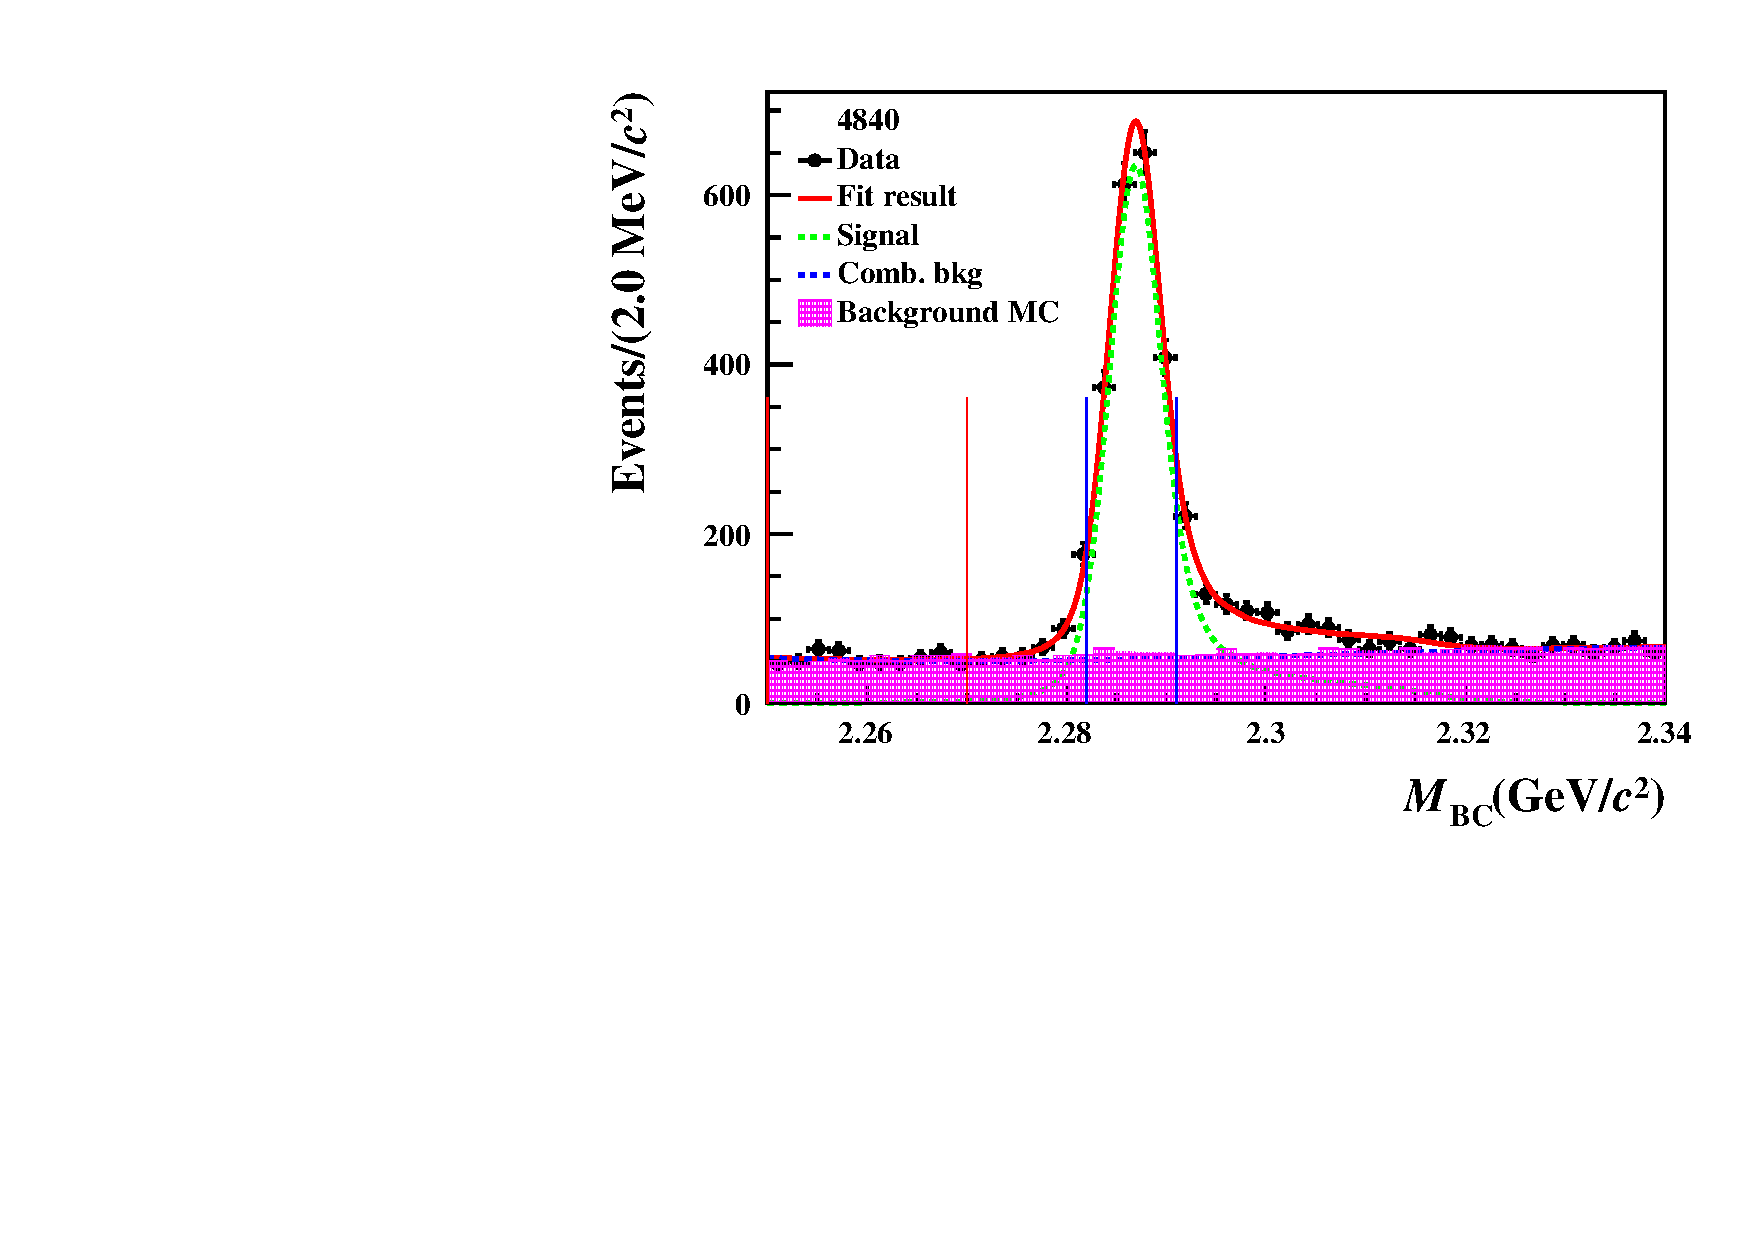
\includegraphics[width=0.24\textwidth]{figure/fit_mbc/fit_mBC_data4840.pdf}
    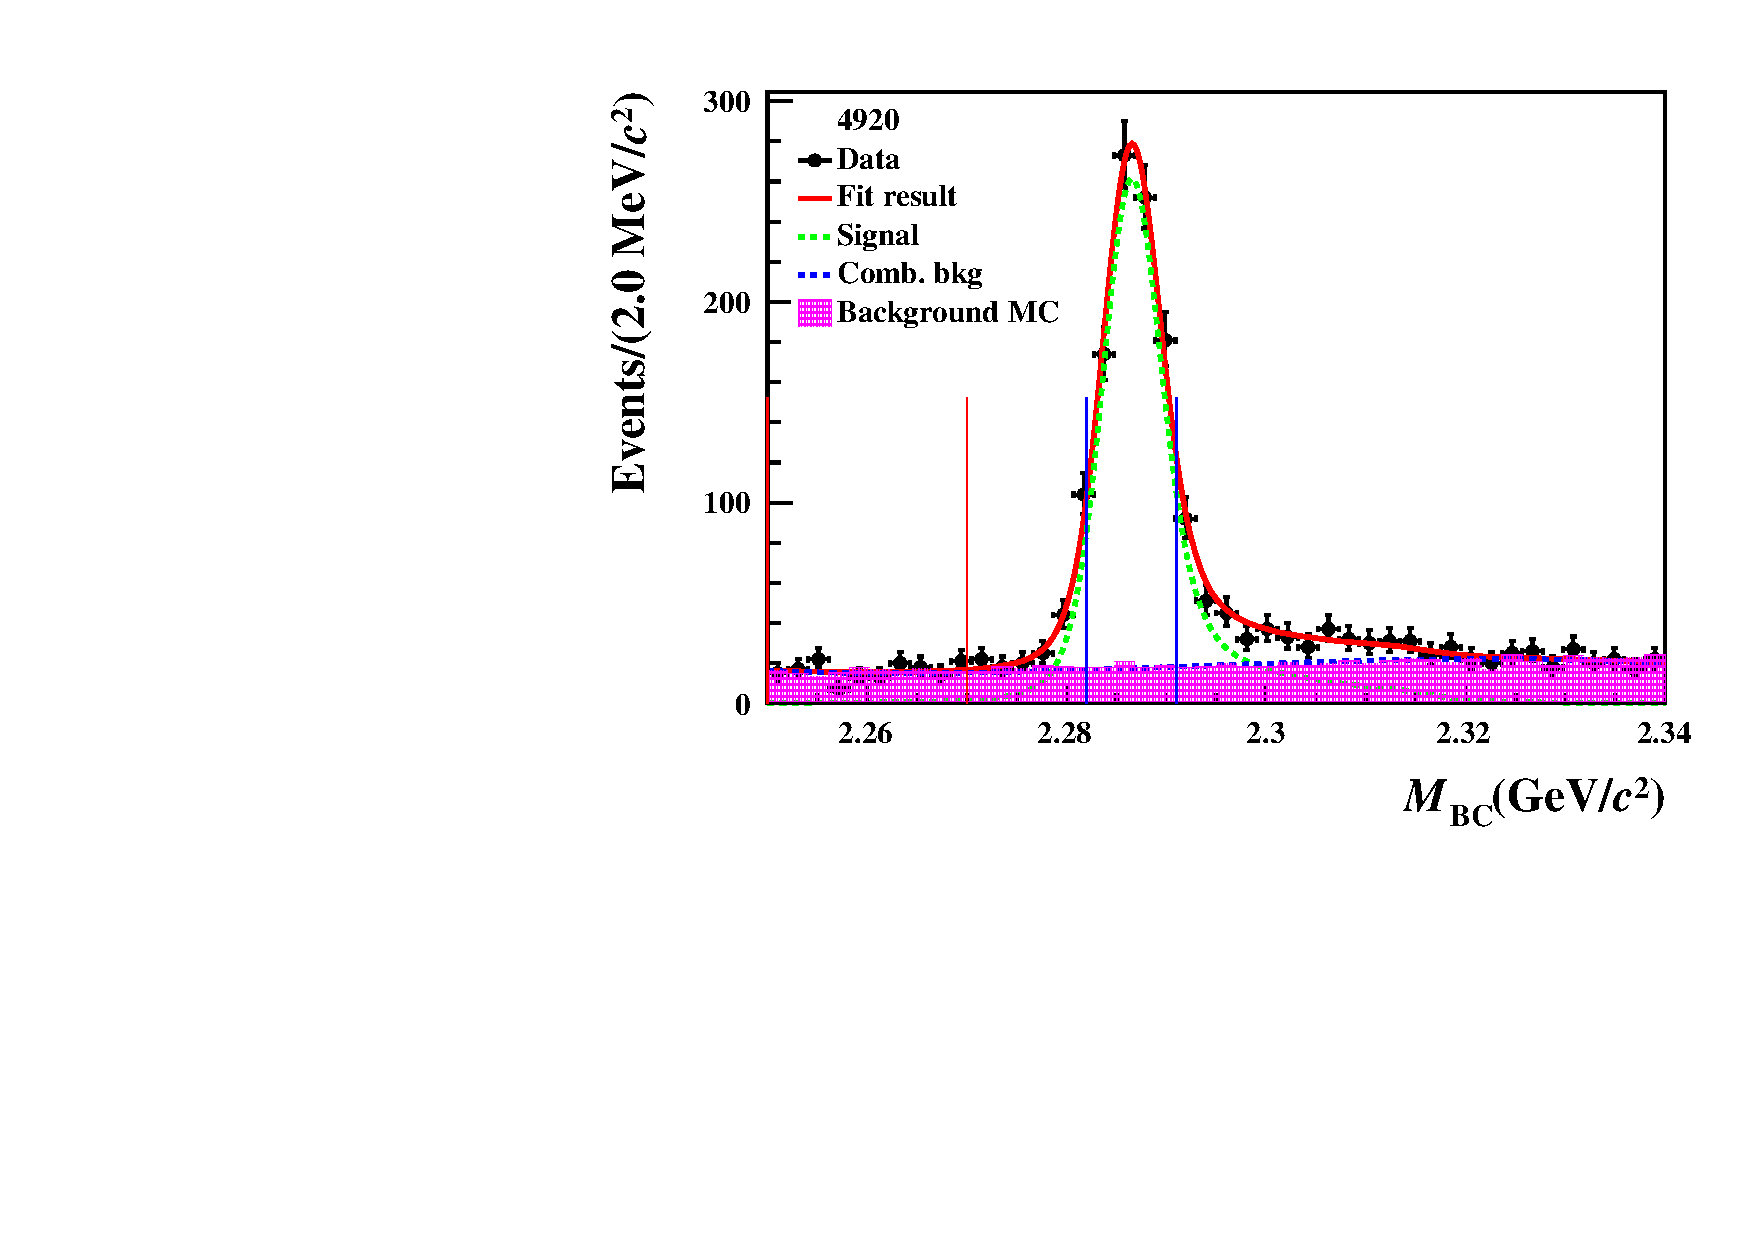
\includegraphics[width=0.24\textwidth]{figure/fit_mbc/fit_mBC_data4914.pdf}
    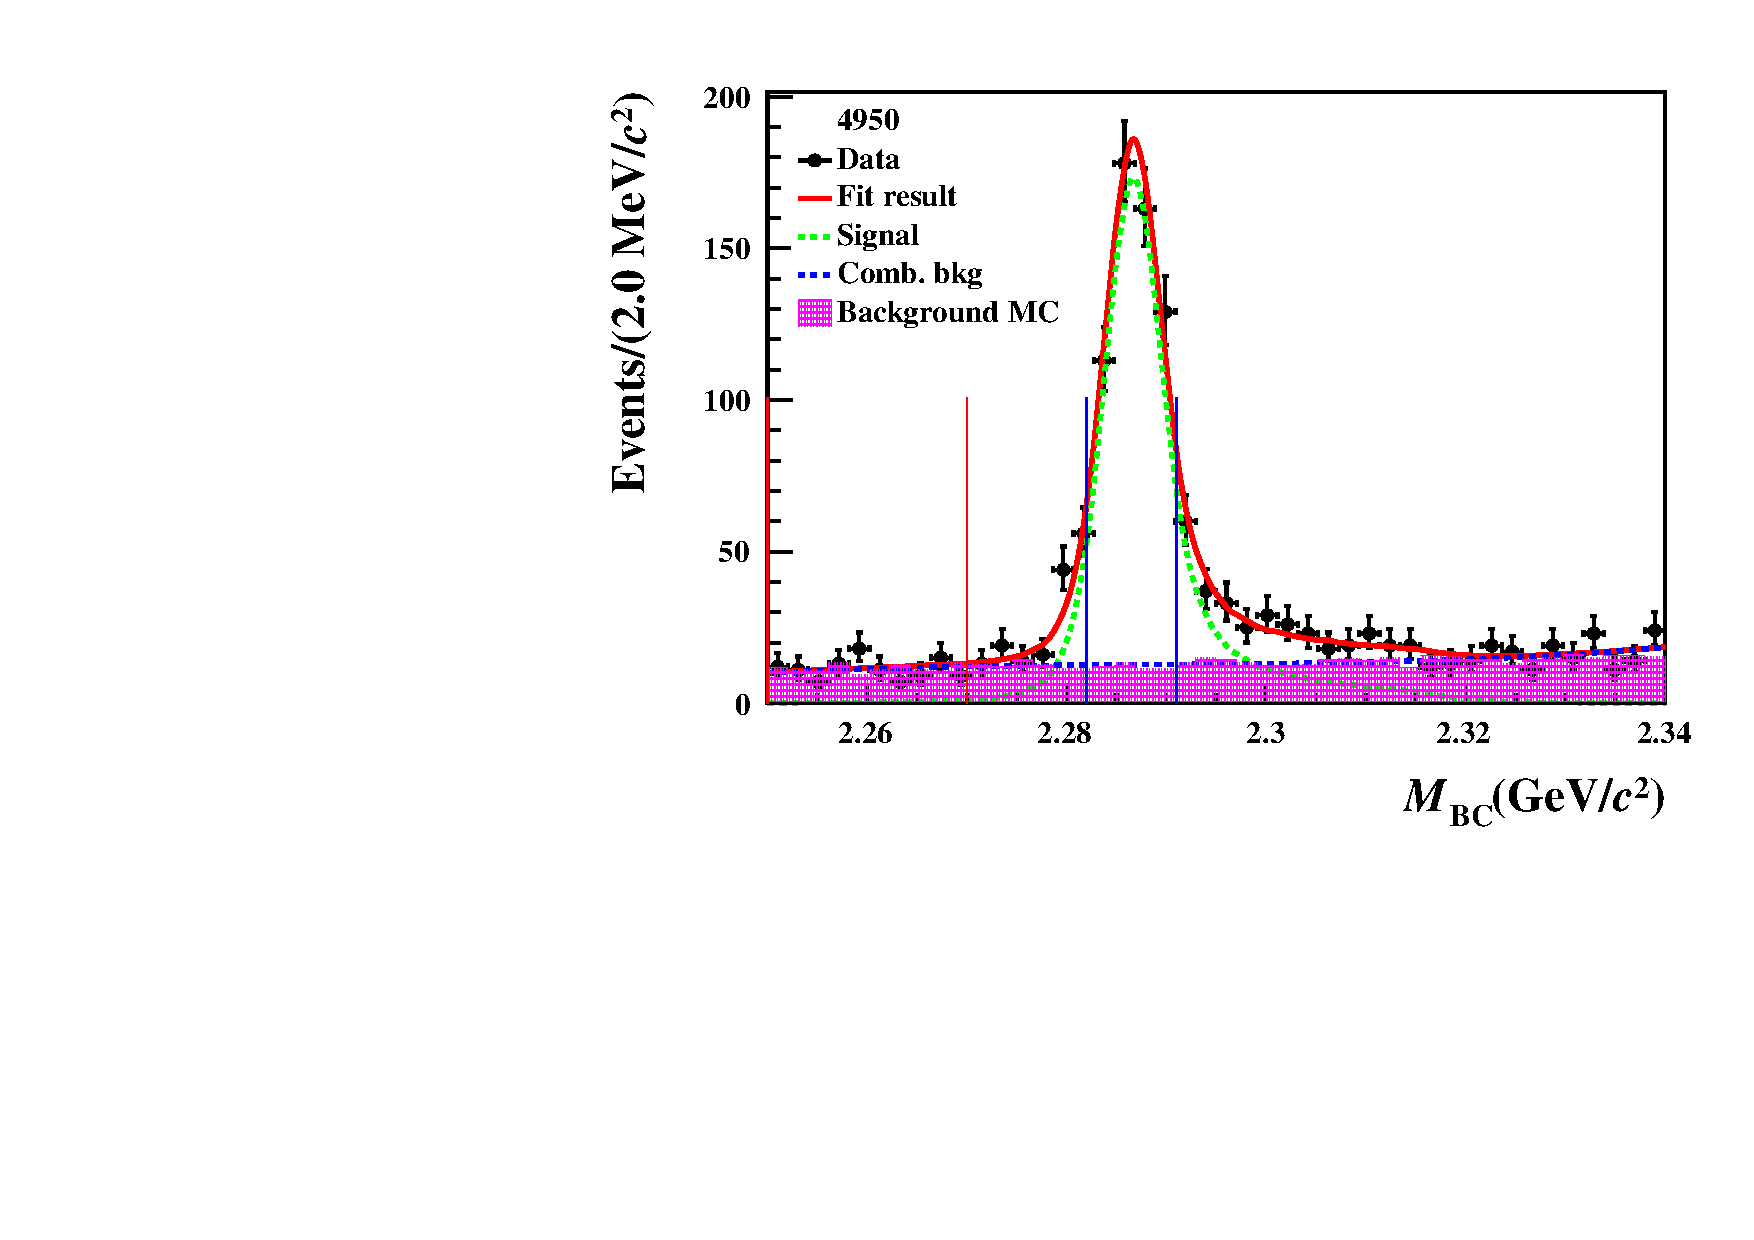
\includegraphics[width=0.24\textwidth]{figure/fit_mbc/fit_mBC_data4946.pdf}
    \caption{Fit results on $\mbc$ distributions for each energy point. The two blue vertical lines indicate the $\mbc$ signal region, and two red vertical lines indicate the $\mbc$ sideband region.}
\label{fig:fit_mbc}
\end{figure}

\begin{table}\centering
    \caption{Fit results within signal regions for each energy point, with $\mbc$ requirements, signal yields, background yields, signal purities, background fractions and convolved Gaussian width values. }
    \label{tab:fit_mbc_results}
    \resizebox{\textwidth}{!}{
    \begin{tabular}{ccccccc}
        \hline\hline
     & Signal region(GeV/$c^2$) & Signal yields & Bkg yields & Signal purity (\%) & Bkg fraction (\%) & Gaussian width (MeV/$c^2$)\\\hline
     4600 & [2.282, 2.291] & 6117$\pm$83 & 327$\pm$10 & 94.9$\pm$0.2 & 5.1$\pm$0.2 & 0.16$\pm$0.06\\
     4612 & [2.282, 2.291] & 1006$\pm$34 & 70$\pm$5 & 93.5$\pm$0.5 & 6.5$\pm$0.5 & 0.03$\pm$0.17\\
     4626 & [2.282, 2.291] & 5044$\pm$76 & 328$\pm$10 & 93.9$\pm$0.2 & 6.1$\pm$0.2 & 0.14$\pm$0.15\\
     4640 & [2.282, 2.291] & 5343$\pm$77 & 336$\pm$10 & 94.1$\pm$0.2 & 5.9$\pm$0.2 & 0.39$\pm$0.11\\
     4660 & [2.282, 2.291] & 4950$\pm$72 & 341$\pm$8 & 93.6$\pm$0.2 & 6.4$\pm$0.2 & 0.44$\pm$0.11\\
     4680 & [2.282, 2.291] & 14302$\pm$121 & 1090$\pm$14 & 92.9$\pm$0.1 & 7.1$\pm$0.1 & 0.46$\pm$0.07\\
     4700 & [2.282, 2.291] & 4168$\pm$65 & 340$\pm$7 & 92.5$\pm$0.2 & 7.5$\pm$0.2 & 0.57$\pm$0.12\\
     4740 & [2.282, 2.291] & 906$\pm$33 & 97$\pm$4 & 90.3$\pm$0.6 & 9.7$\pm$0.6 & 0.87$\pm$0.24\\
     4750 & [2.282, 2.291] & 2116$\pm$51 & 211$\pm$6 & 90.9$\pm$0.4 & 9.1$\pm$0.4 & 0.42$\pm$0.27\\
     4780 & [2.282, 2.291] & 2846$\pm$58 & 255$\pm$7 & 91.8$\pm$0.3 & 8.2$\pm$0.3 & 0.88$\pm$0.15\\
     4840 & [2.282, 2.291] & 1900$\pm$49 & 229$\pm$6 & 89.3$\pm$0.4 & 10.7$\pm$0.4 & 0.79$\pm$0.24\\
     4920 & [2.282, 2.291] & 844$\pm$31 & 77$\pm$4 & 91.7$\pm$0.6 & 8.3$\pm$0.6 & 0.92$\pm$0.36\\
     4950 & [2.282, 2.291] & 553$\pm$25 & 56$\pm$3 & 90.8$\pm$0.7 & 9.2$\pm$0.7 & 0.05$\pm$2.89\\
    \hline\hline
    \end{tabular}
    }
\end{table}

\subsection{Check of sideband regions}
\label{sec:sideband_check}

After applying all selection criteria, an additional kinematic fit is performed to improve the momentum resolution of particles for the amplitude analysis. The kinematic constraints are listed below:
\begin{itemize}
    \item Signal side $\lcp$, reconstructed by $p$, $K^-$ and $\pi^+$ is constrained at the $\Lambda_c$ nominal mass value,
    \item Recoil side $\lcm$ is constrained at the $\Lambda_c$ nominal mass value using information of initial four-momentum of $e^+e^-$ collision.
\end{itemize}

In the amplitude analysis, the background contributions are modeled by the data events in the $\mbc$ sideband region, scaled according to the background fractions from the $\mbc$ fit. It is crucial to valid the consistency of the background shape between the $\mbc$ sideband region and signal region. Shapes of $M^2(pK^-)$, $M^2(p\pi^+)$ and $M^2(K^-\pi^+)$ are compared using the data events and cocktail MC samples with signal process vetoed. Figure~\ref{fig:comp_mc_sideband} shows the shape comparison for cocktail MC samples in the $\mbc$ signal and sideband regions. The distributions of $M^2(pK^-)$ and $M^2(p\pi^+)$ in the $\mbc$ signal and sideband regions agree well with each other within uncertainties. Discrepancy is observed in the distribution of $M^2(K^-\pi^+)$. 
Figure~\ref{fig:comp_datamc_sideband} shows the comparison results between data and cocktail MC in the $\mbc$ sideband region. Visible difference can be observed in the distribution of $M^2(K^-\pi^+)$, which arises from the lack of modelling on $\bar{K}^*$ processes in the cocktail MC samples. In the nominal amplitude analysis, we still trust data and use data events in $\mbc$ sideband region to describe the background. The observed disagreements in the Figure~\ref{fig:comp_mc_sideband}, \ref{fig:comp_datamc_sideband} will be considered for possible variations of the background shape in the study of systematic uncertainties. More details about the source of background are documented in Appendix~\ref{app:bkg_check}.

\begin{figure}[H]\centering
    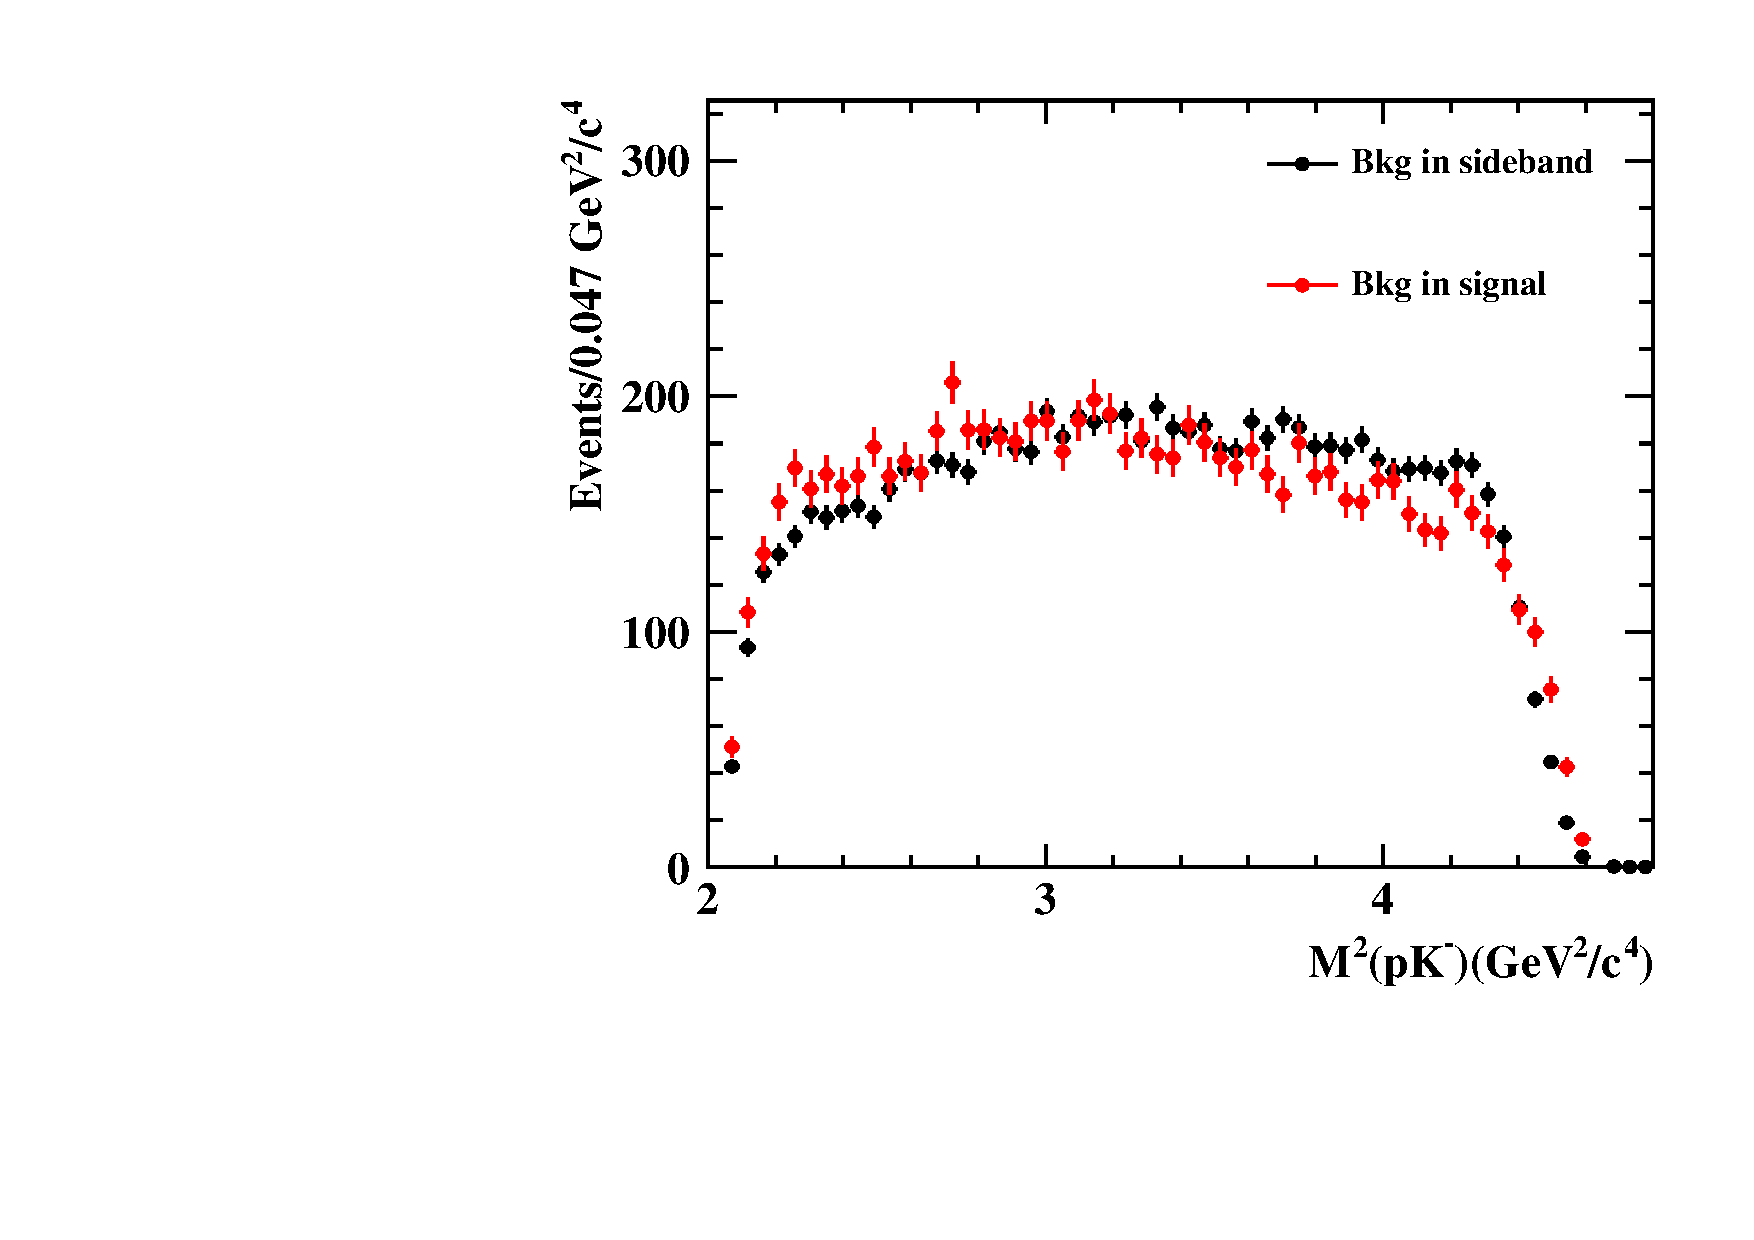
\includegraphics[width=0.325\textwidth]{figure/sideband/output_mc_0_sideband_signal_m2_12_2c_1.pdf}
    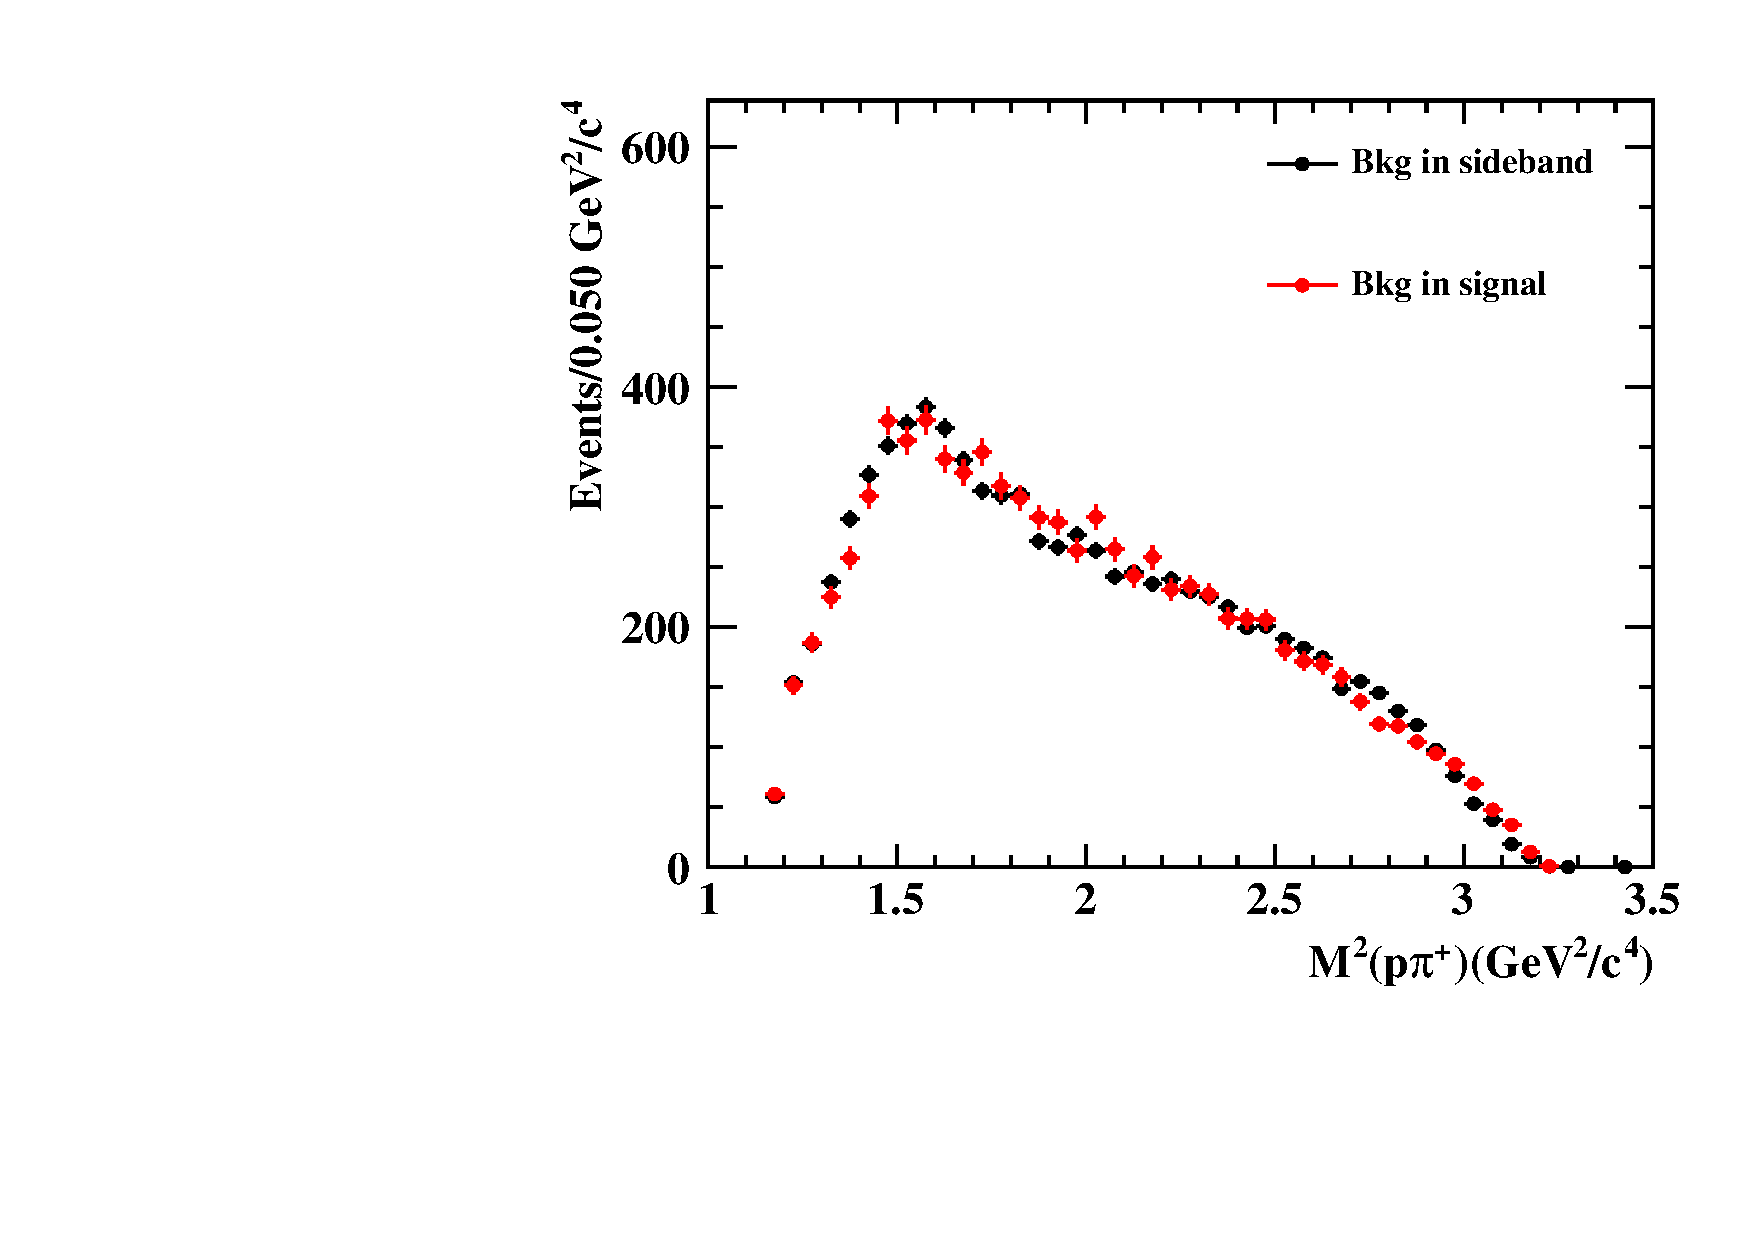
\includegraphics[width=0.325\textwidth]{figure/sideband/output_mc_0_sideband_signal_m2_13_2c_1.pdf}
    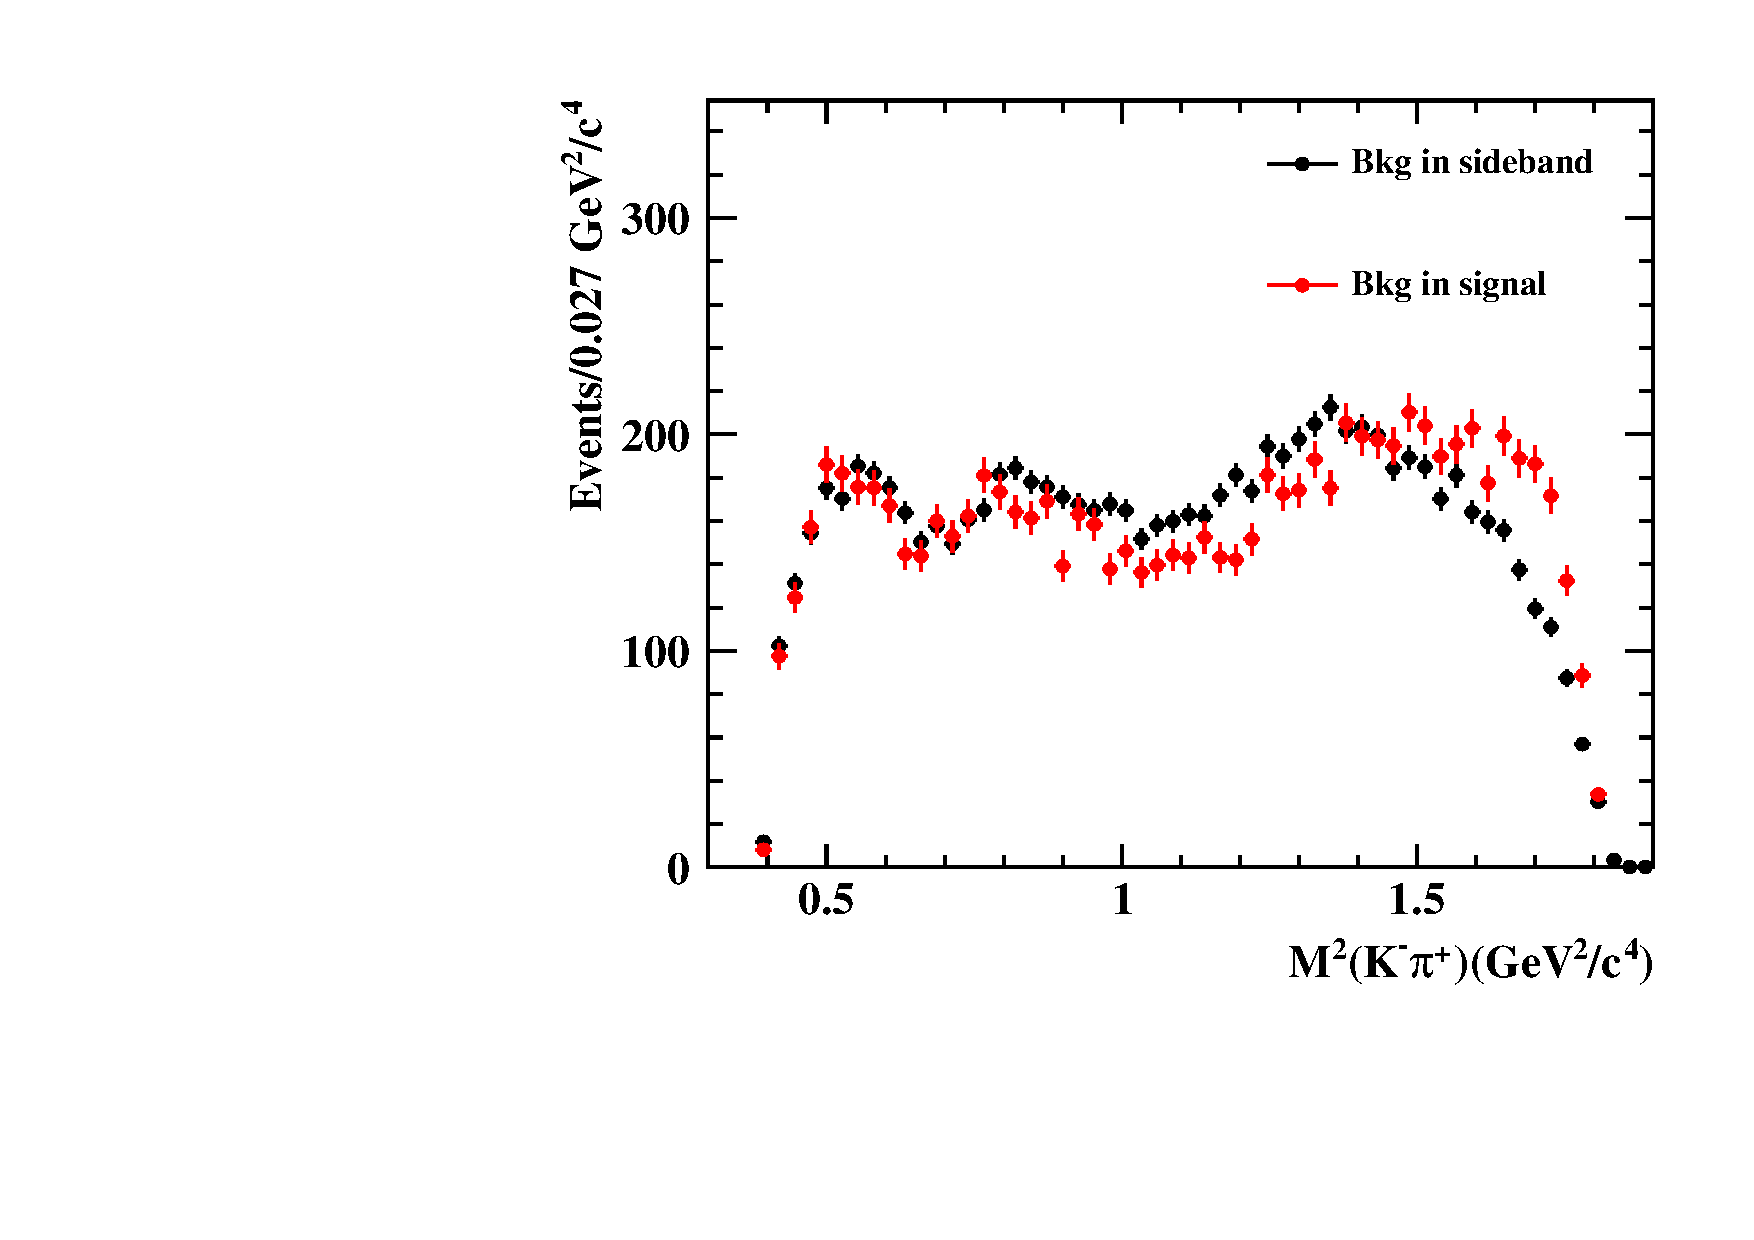
\includegraphics[width=0.325\textwidth]{figure/sideband/output_mc_0_sideband_signal_m2_23_2c_1.pdf}
    \caption{Shape comparison of $M^2(pK^-)$ (left), $M^2(p\pi^+)$ (middle) and $M^2(K^-\pi^+)$ (right) of cocktail MC samples between the $\mbc$ sideband and signal regions.}
\label{fig:comp_mc_sideband}
\end{figure}

\begin{figure}[H]\centering
    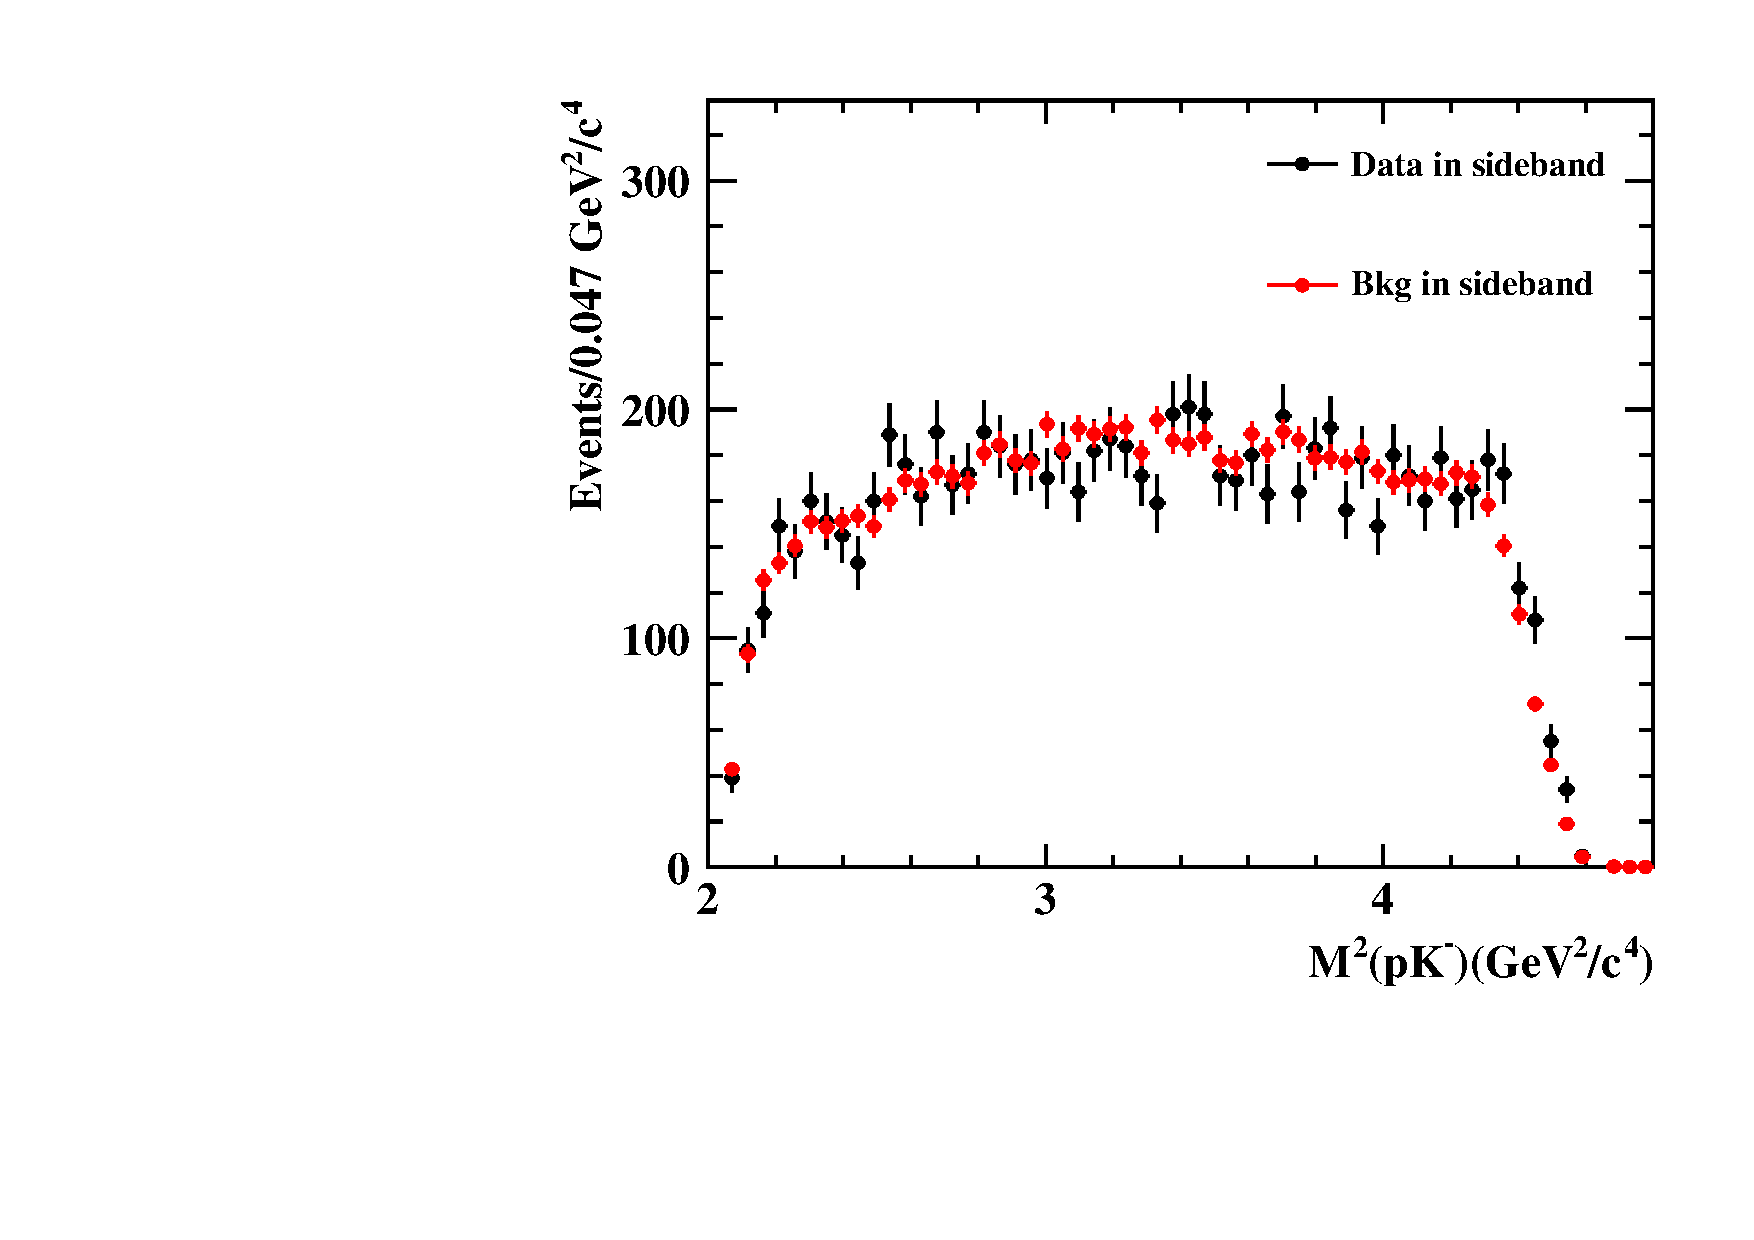
\includegraphics[width=0.325\textwidth]{figure/sideband/output_data_mc_0_sideband_m2_12_2c_1.pdf}
    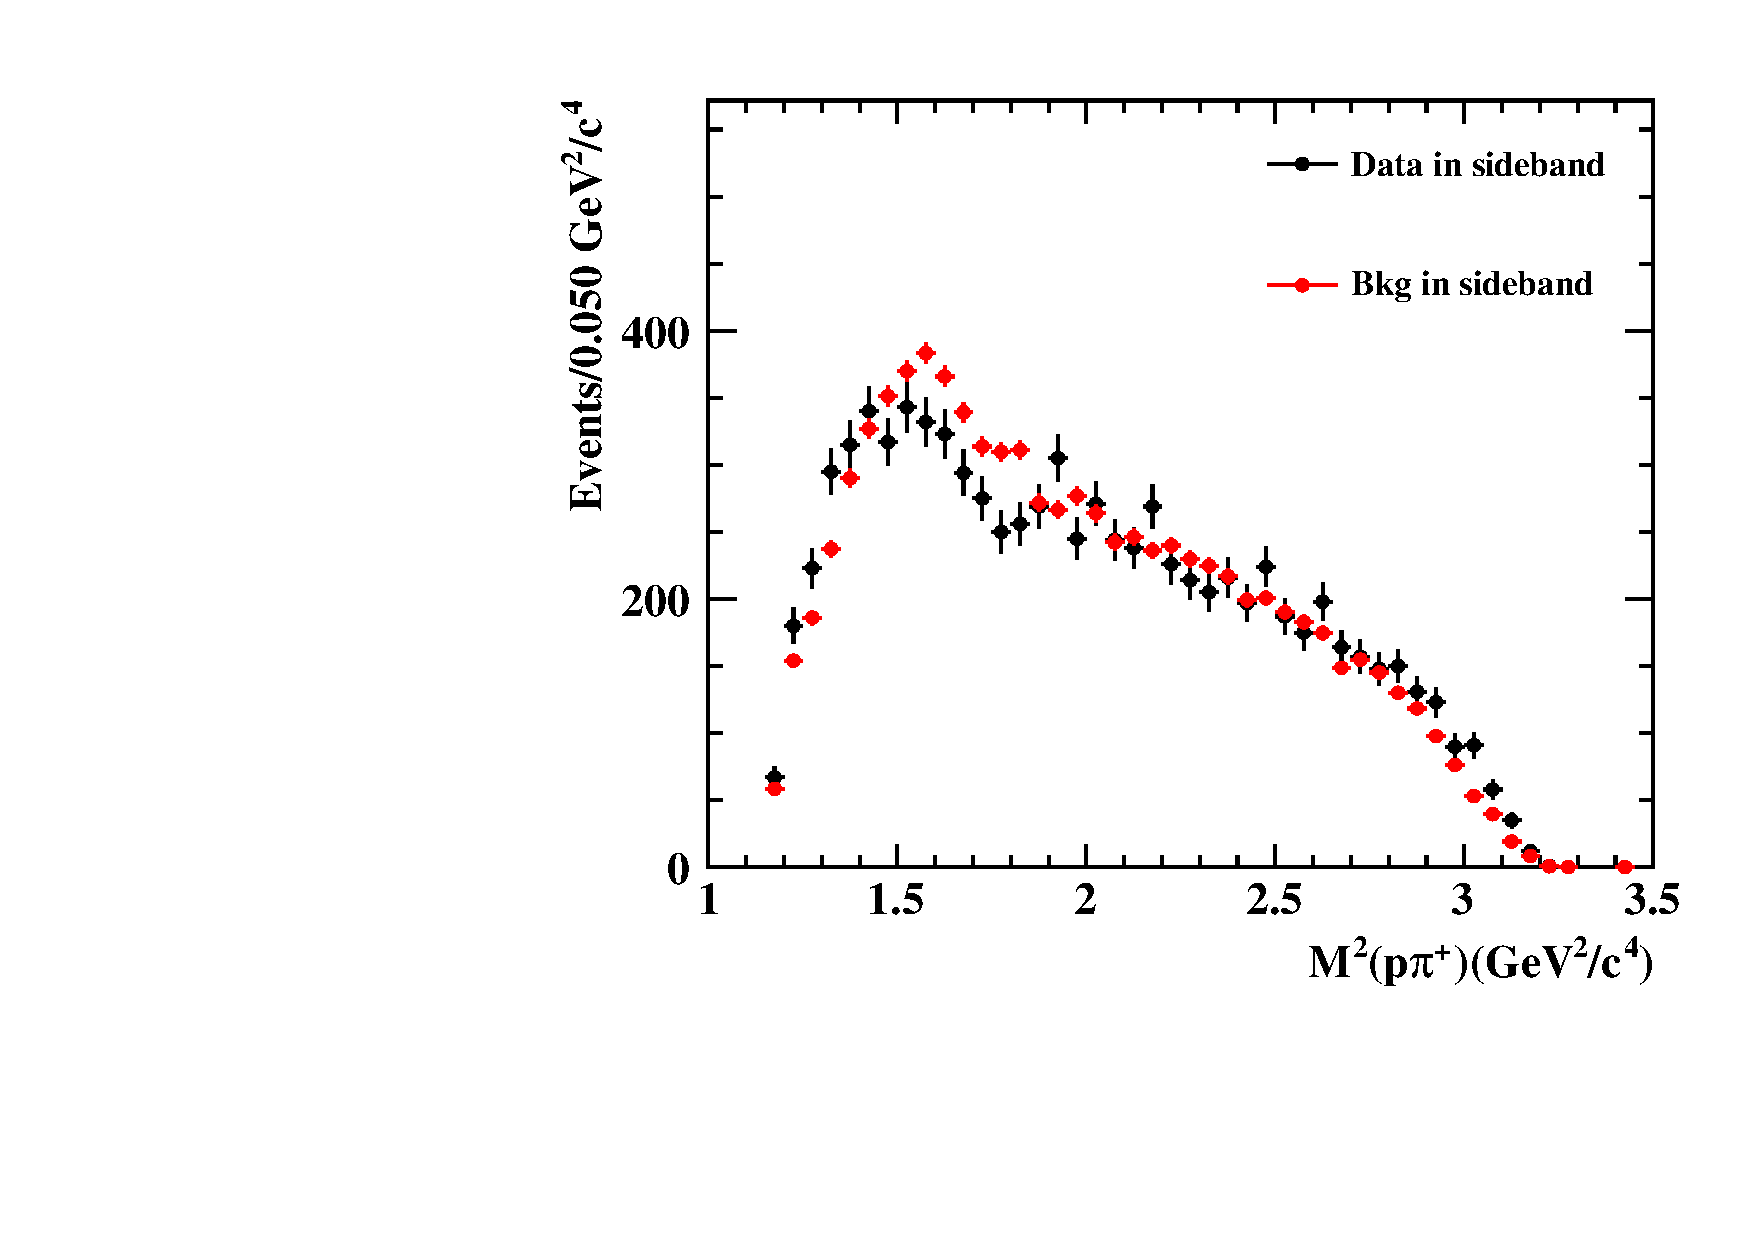
\includegraphics[width=0.325\textwidth]{figure/sideband/output_data_mc_0_sideband_m2_13_2c_1.pdf}
    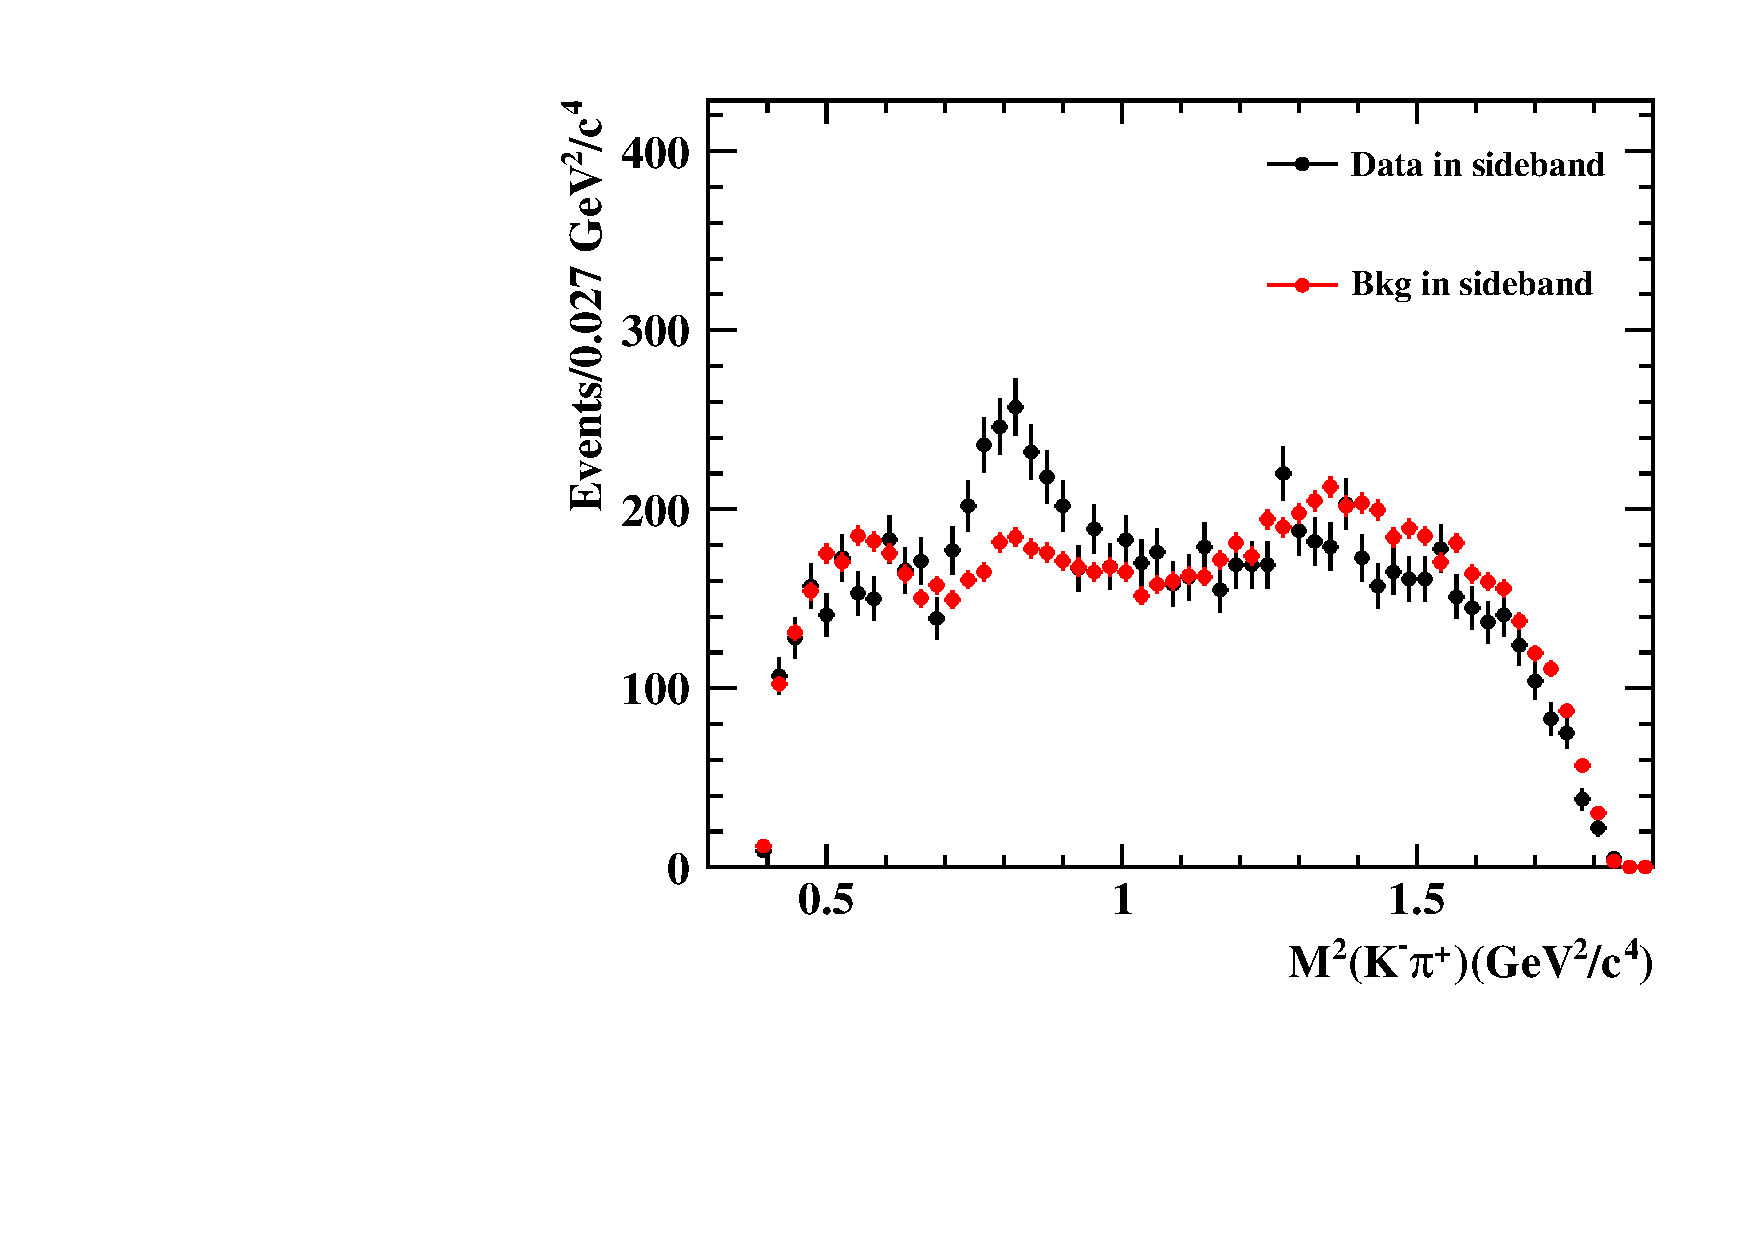
\includegraphics[width=0.325\textwidth]{figure/sideband/output_data_mc_0_sideband_m2_23_2c_1.pdf}
    \caption{Shape comparison of $M^2(pK^-)$ (left), $M^2(p\pi^+)$ (middle) and $M^2(K^-\pi^+)$ (right) between data and cocktail MC in the $\mbc$ sideband region.}
\label{fig:comp_datamc_sideband}
\end{figure}
\clearpage
\section{Amplitude analysis of $\lcp \to p K^- \pi^+$}
\label{sec:pwa}

After applying all selection criteria and kinematic fit mentioned in Section~\ref{sec:selections}, Dalitz plots combining all 13 energy points are shown in Figure~\ref{fig:daltiz_plots} for $M^2(pK^-)$ and $M^2(K^-\pi^+)$ in the $\mbc$ signal region ($\mbc \in (2.282, 2.291)\gev/c^2$) and sideband region ($\mbc \in (2.25, 2.27)\gev/c^2$). Figure~\ref{fig:projected_plots} shows the spectra for squared two-body invariant mass and polar angles for three charged tracks. Events fall outside of the Daltiz boundaries are excluded due to failure of the kinematic fit with large $\chi^2$. The signal efficiency of the boundary requirements is nearly 100\% with about 0.1\% of data $\mbc$ sideband events excluded. The contributions from intermediate resonances are clearly observed in all three pairs of final states. Multiple $\Lambda^*$, $\Delta^{++}$ and $\overline{K}^*$ resonances are clearly visible in the $pK^-$, $p\pi^+$ and $K^-\pi^+$ final states. 

\begin{figure}[h]\centering
    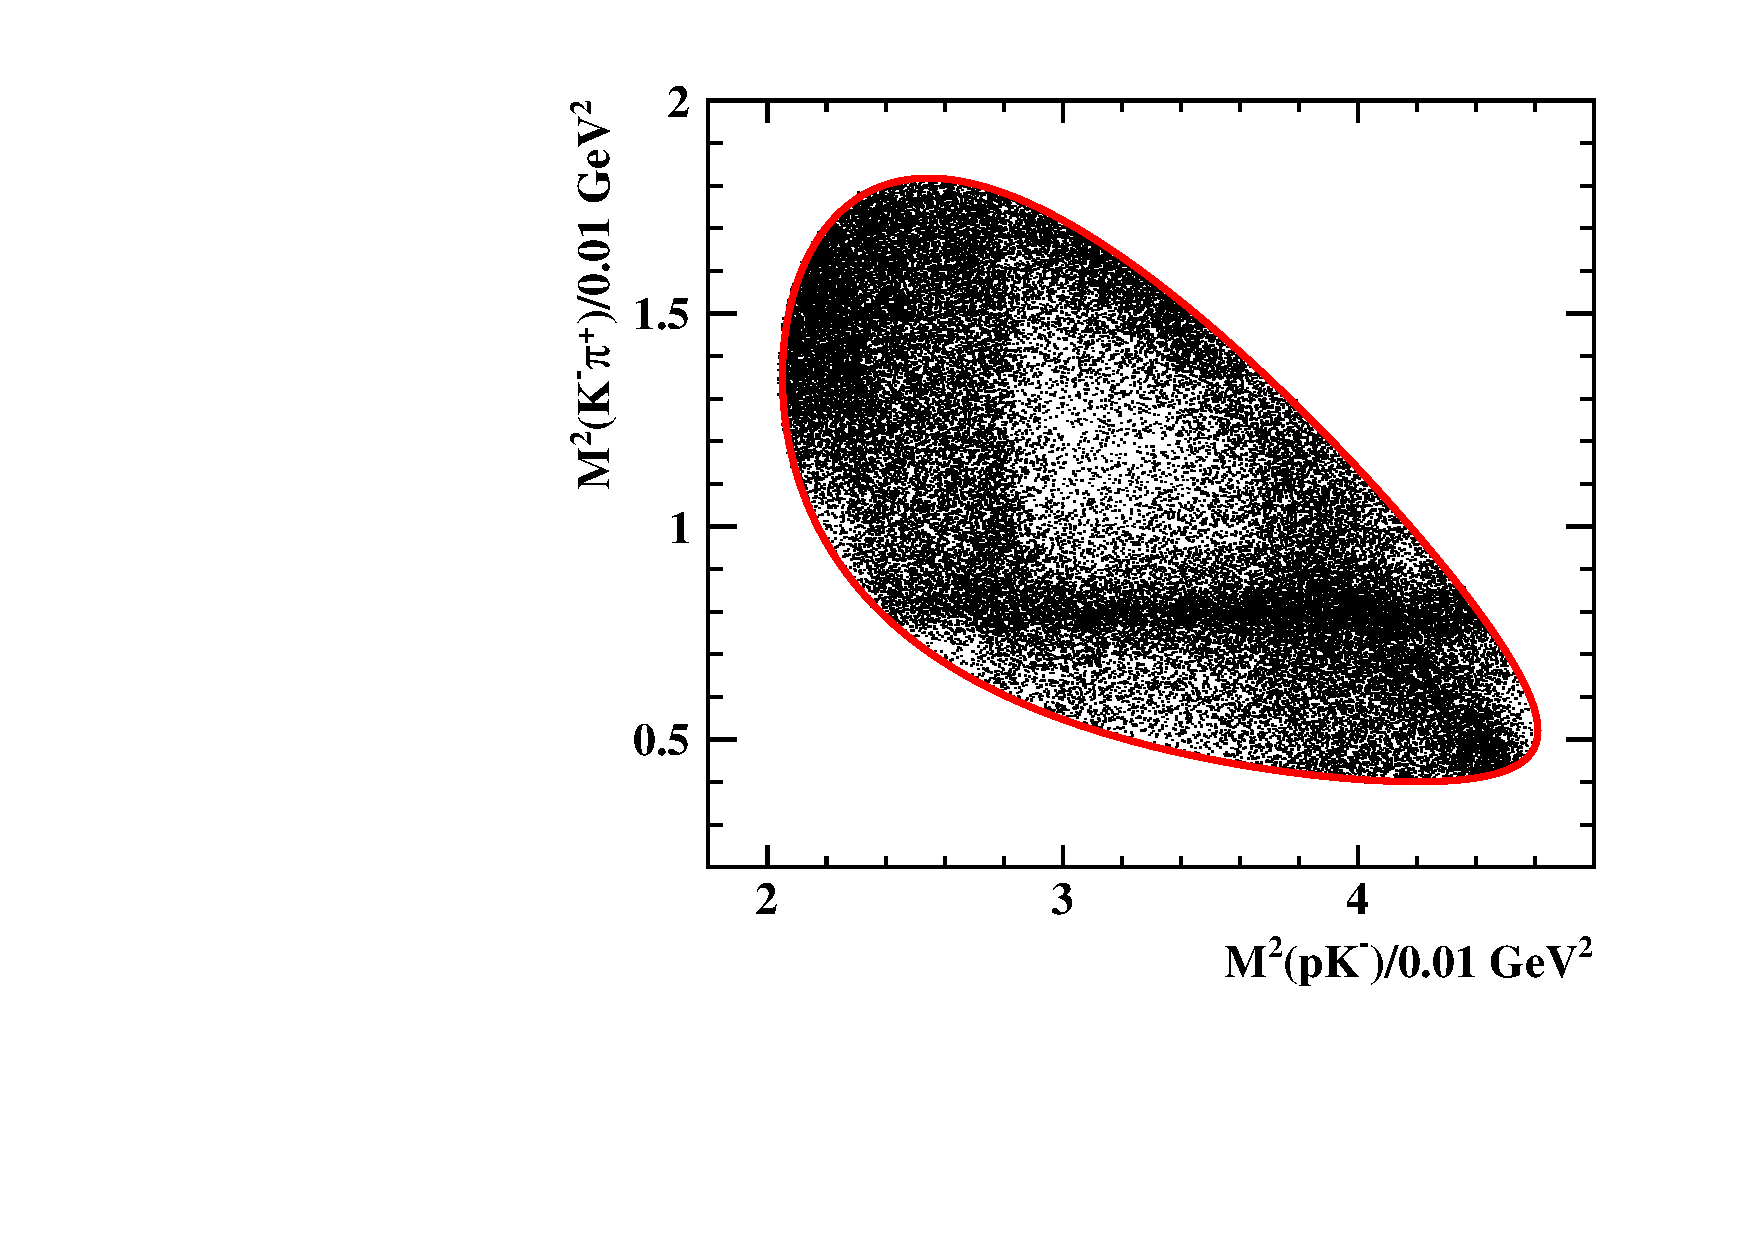
\includegraphics[width=0.48\textwidth]{figure/dalitz/dalitz_Signal_total.pdf}
    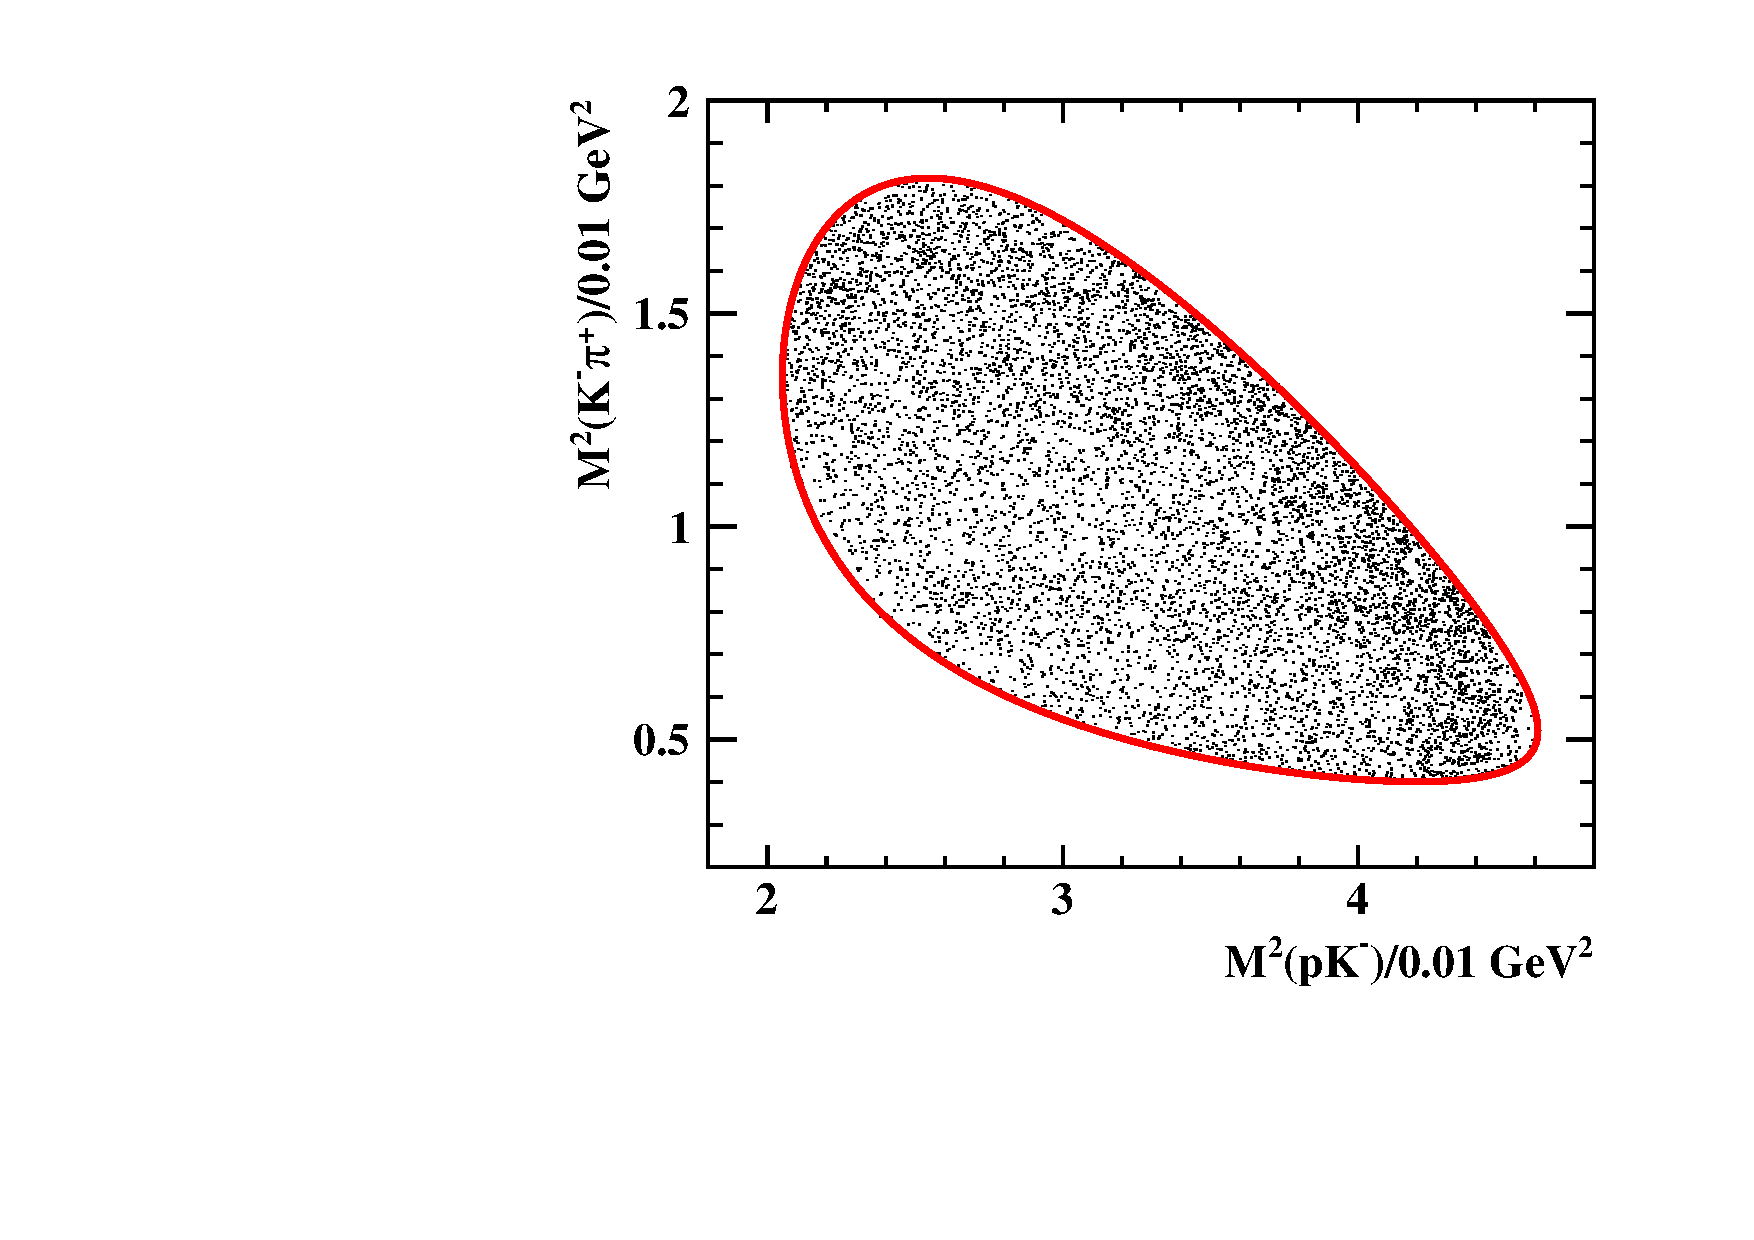
\includegraphics[width=0.48\textwidth]{figure/dalitz/dalitz_Sideband_total.pdf}
    \caption{Dalitz plots for for $M^2(pK^-)$ and $M^2(K^-\pi^+)$ combining all 13 energy points in the $\mbc$ signal region (left) and sideband region (right).}
\label{fig:daltiz_plots}
\end{figure}

\begin{figure}[H]\centering
    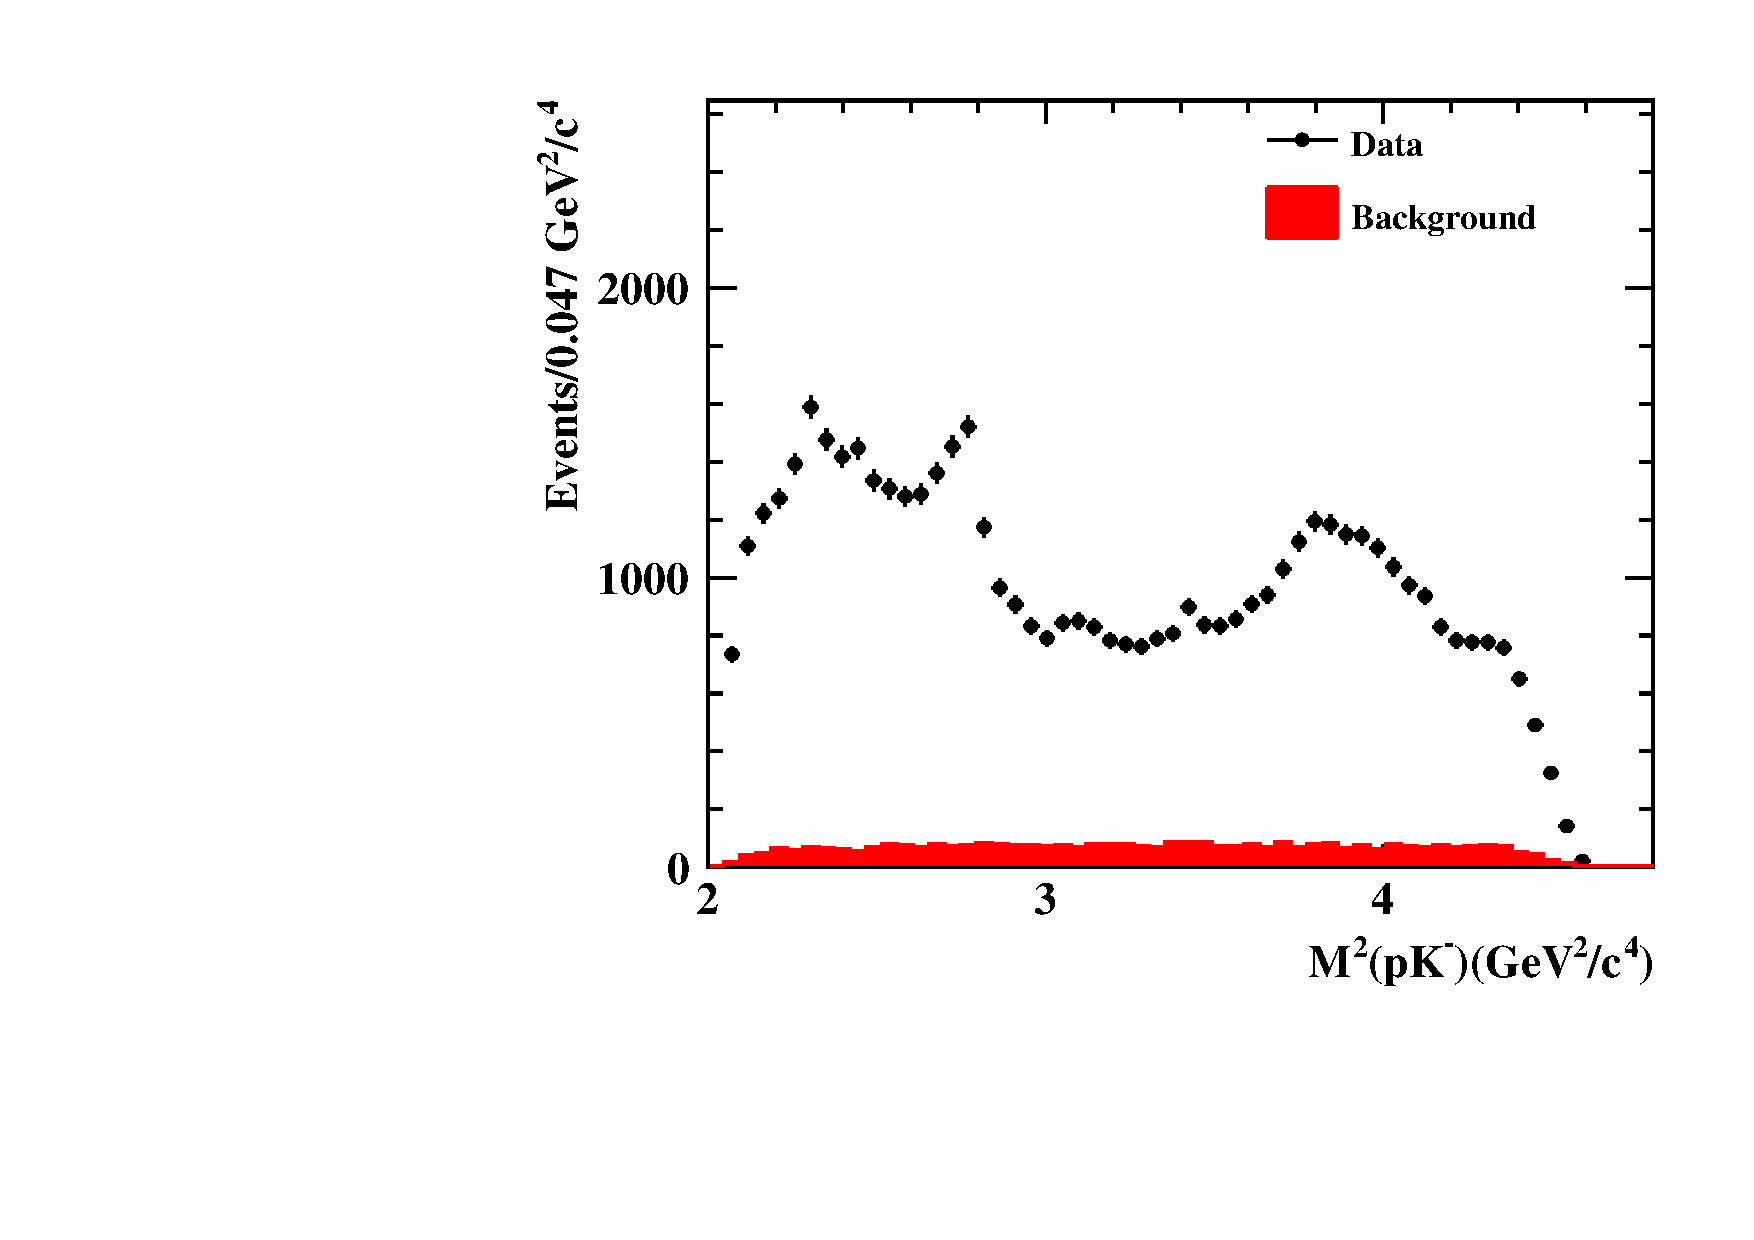
\includegraphics[width=0.32\textwidth]{figure/dalitz/output_data_mc_0_sideband_m2_12_2c_1.pdf}
    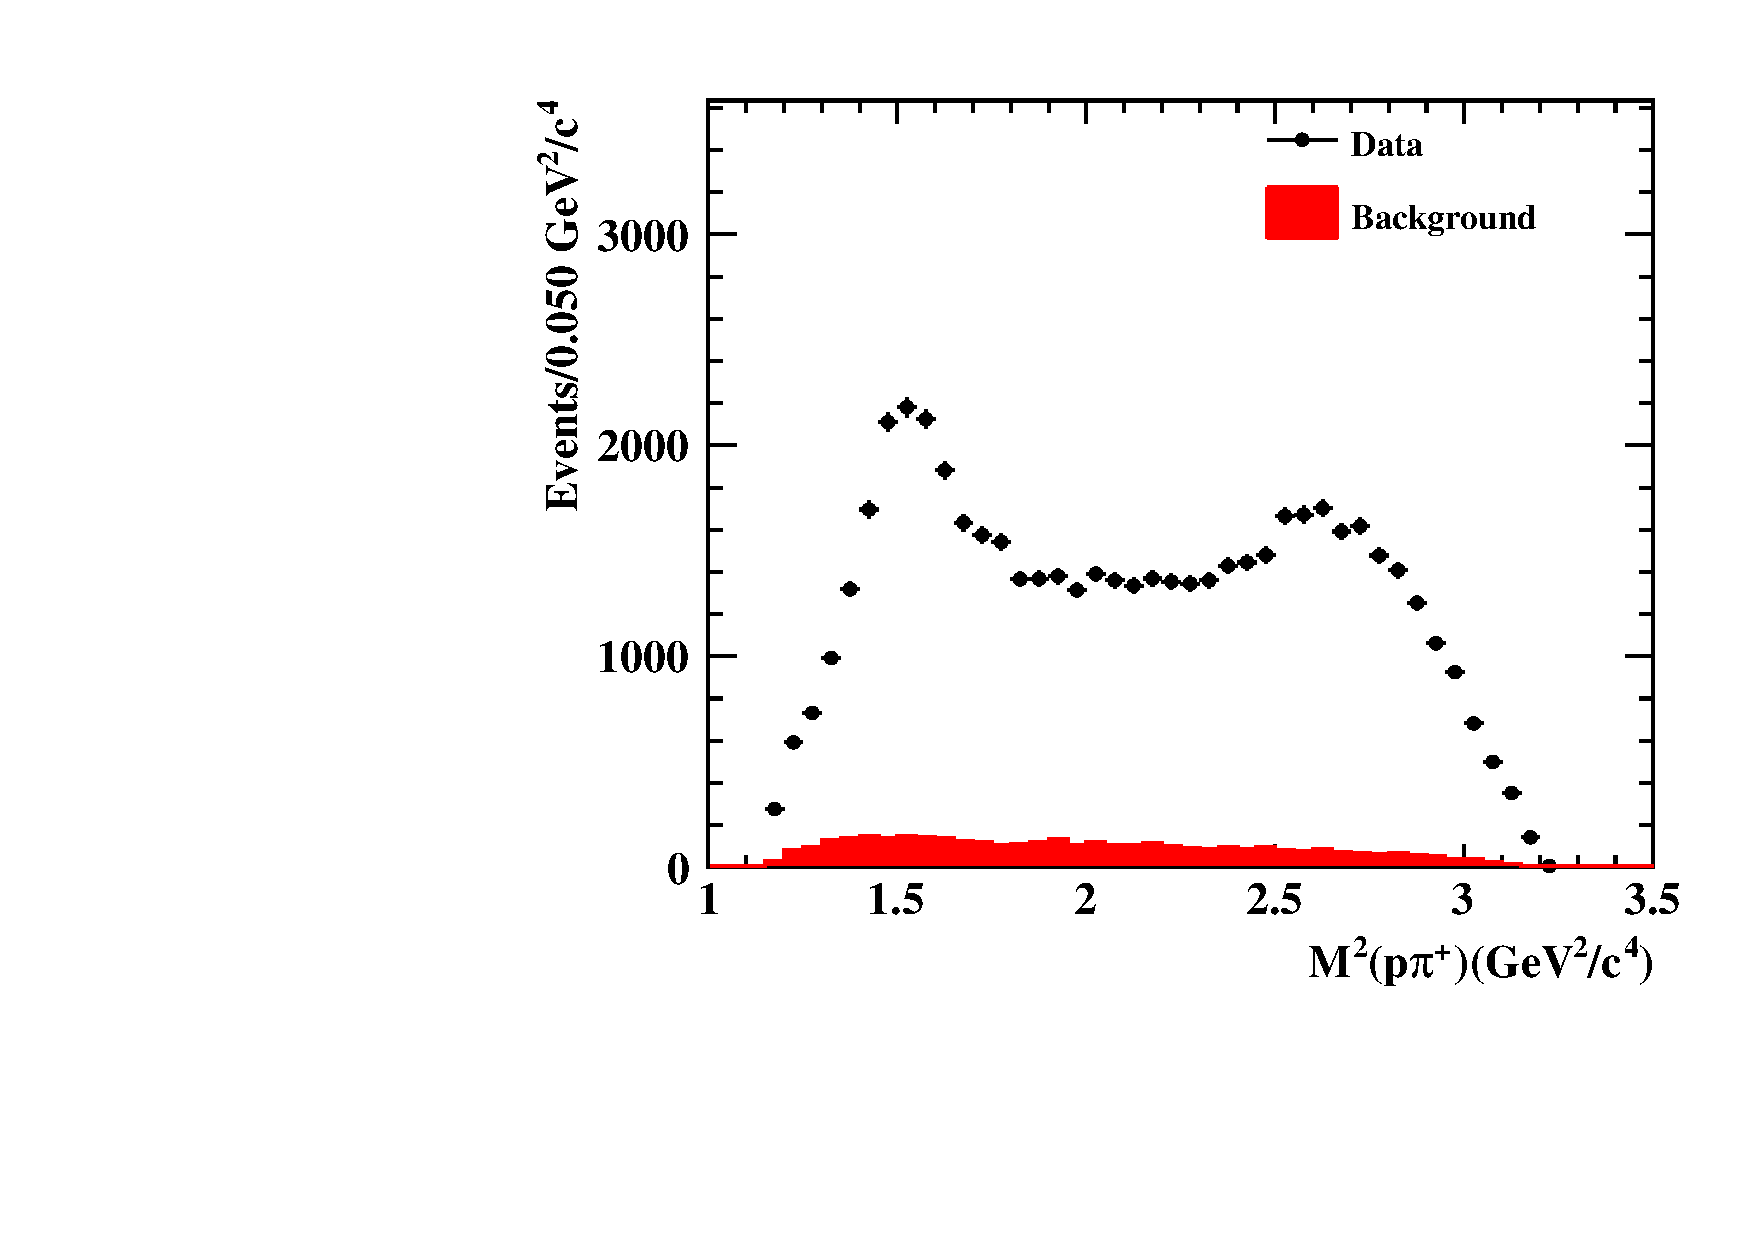
\includegraphics[width=0.32\textwidth]{figure/dalitz/output_data_mc_0_sideband_m2_13_2c_1.pdf}
    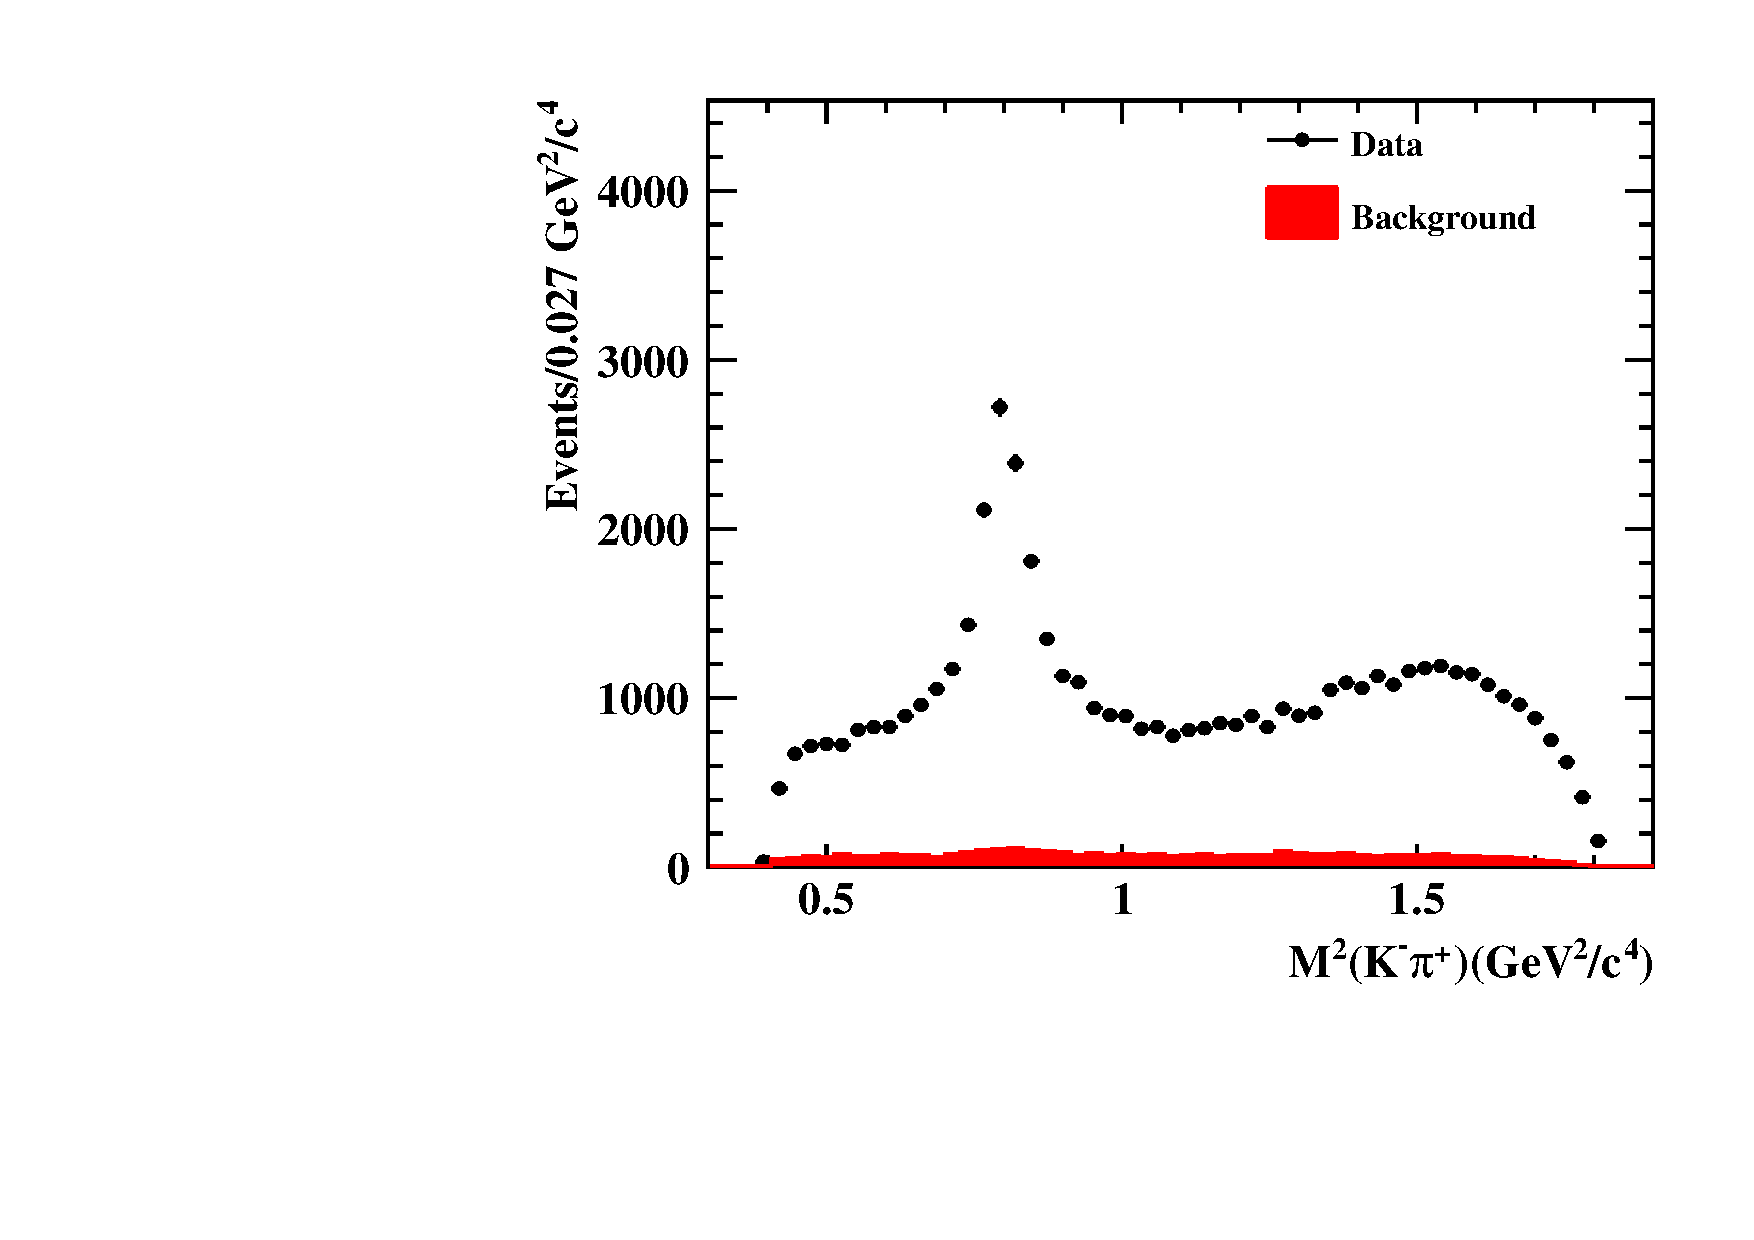
\includegraphics[width=0.32\textwidth]{figure/dalitz/output_data_mc_0_sideband_m2_23_2c_1.pdf}
    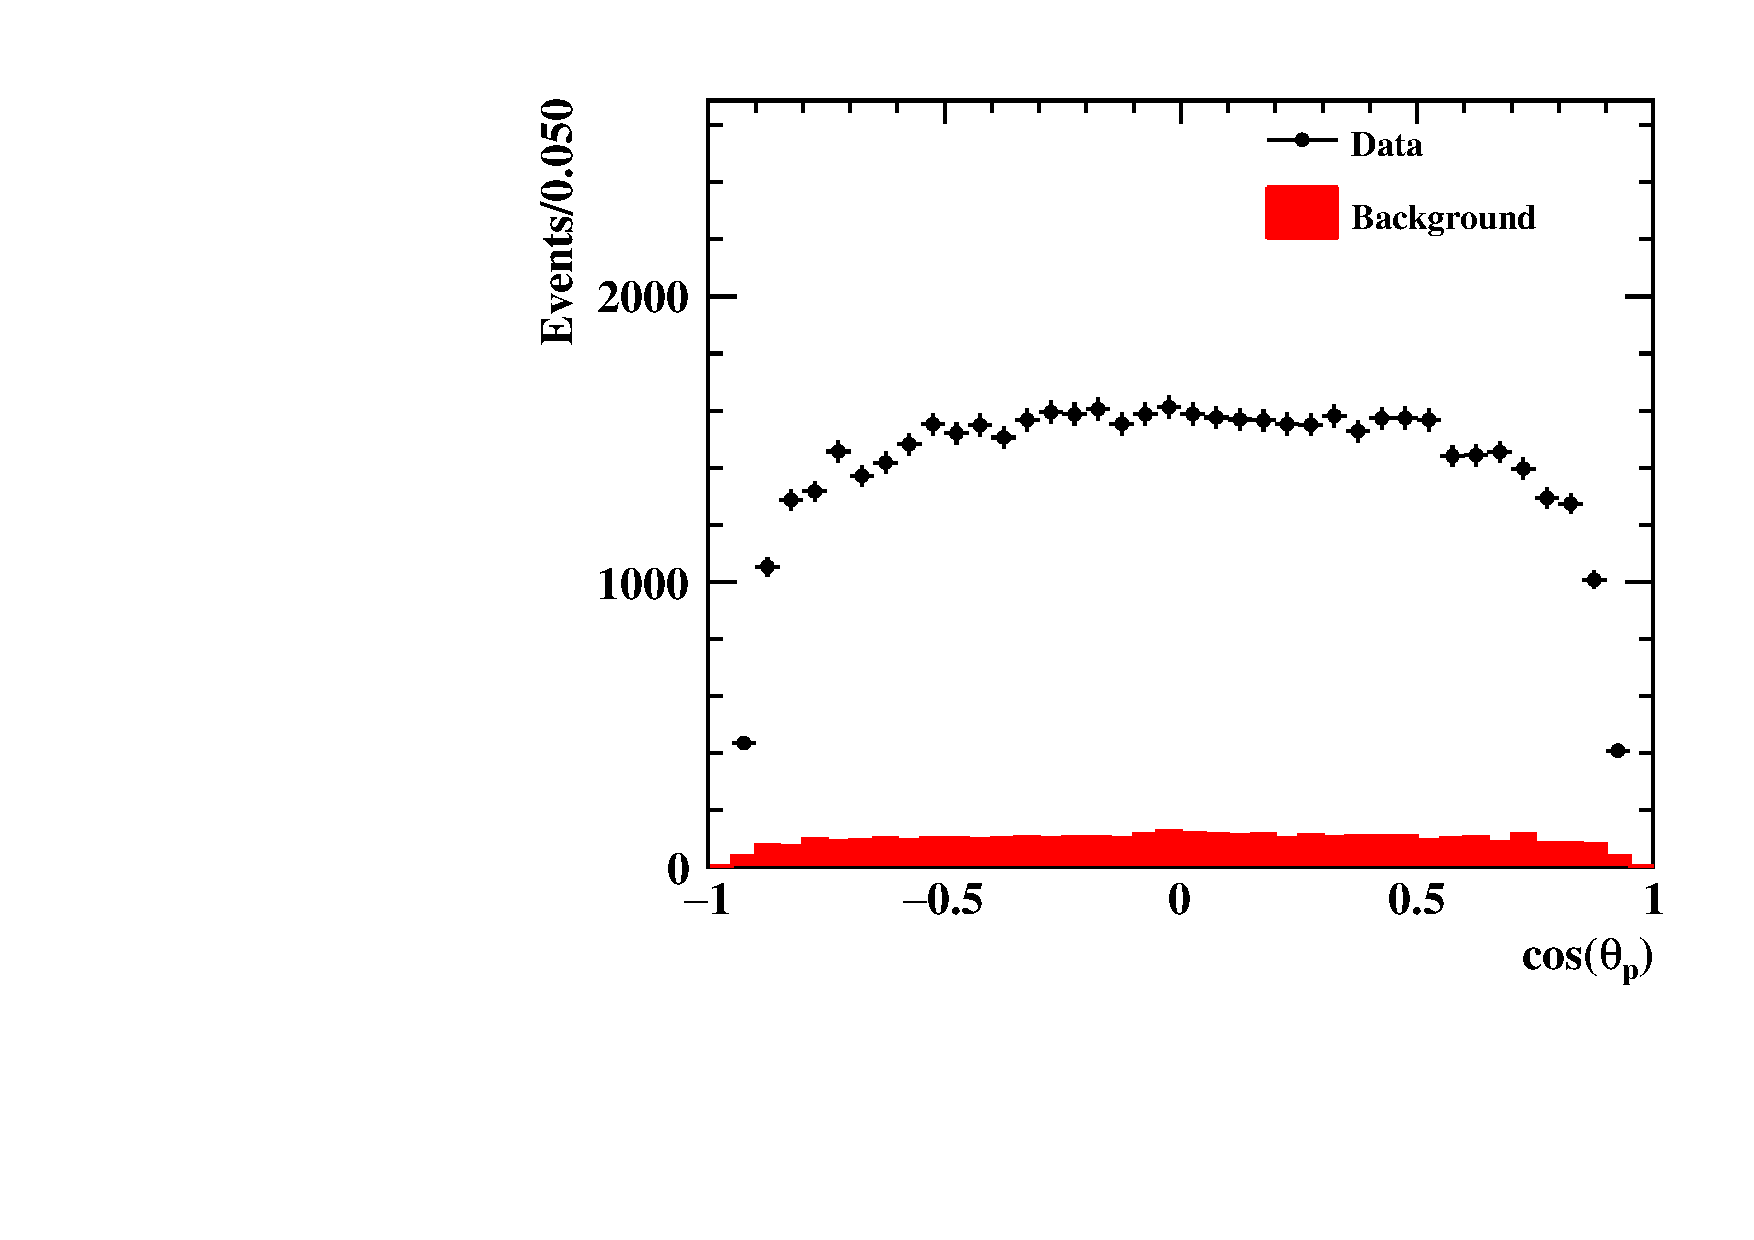
\includegraphics[width=0.32\textwidth]{figure/dalitz/output_data_mc_0_sideband_costheta1_1.pdf}
    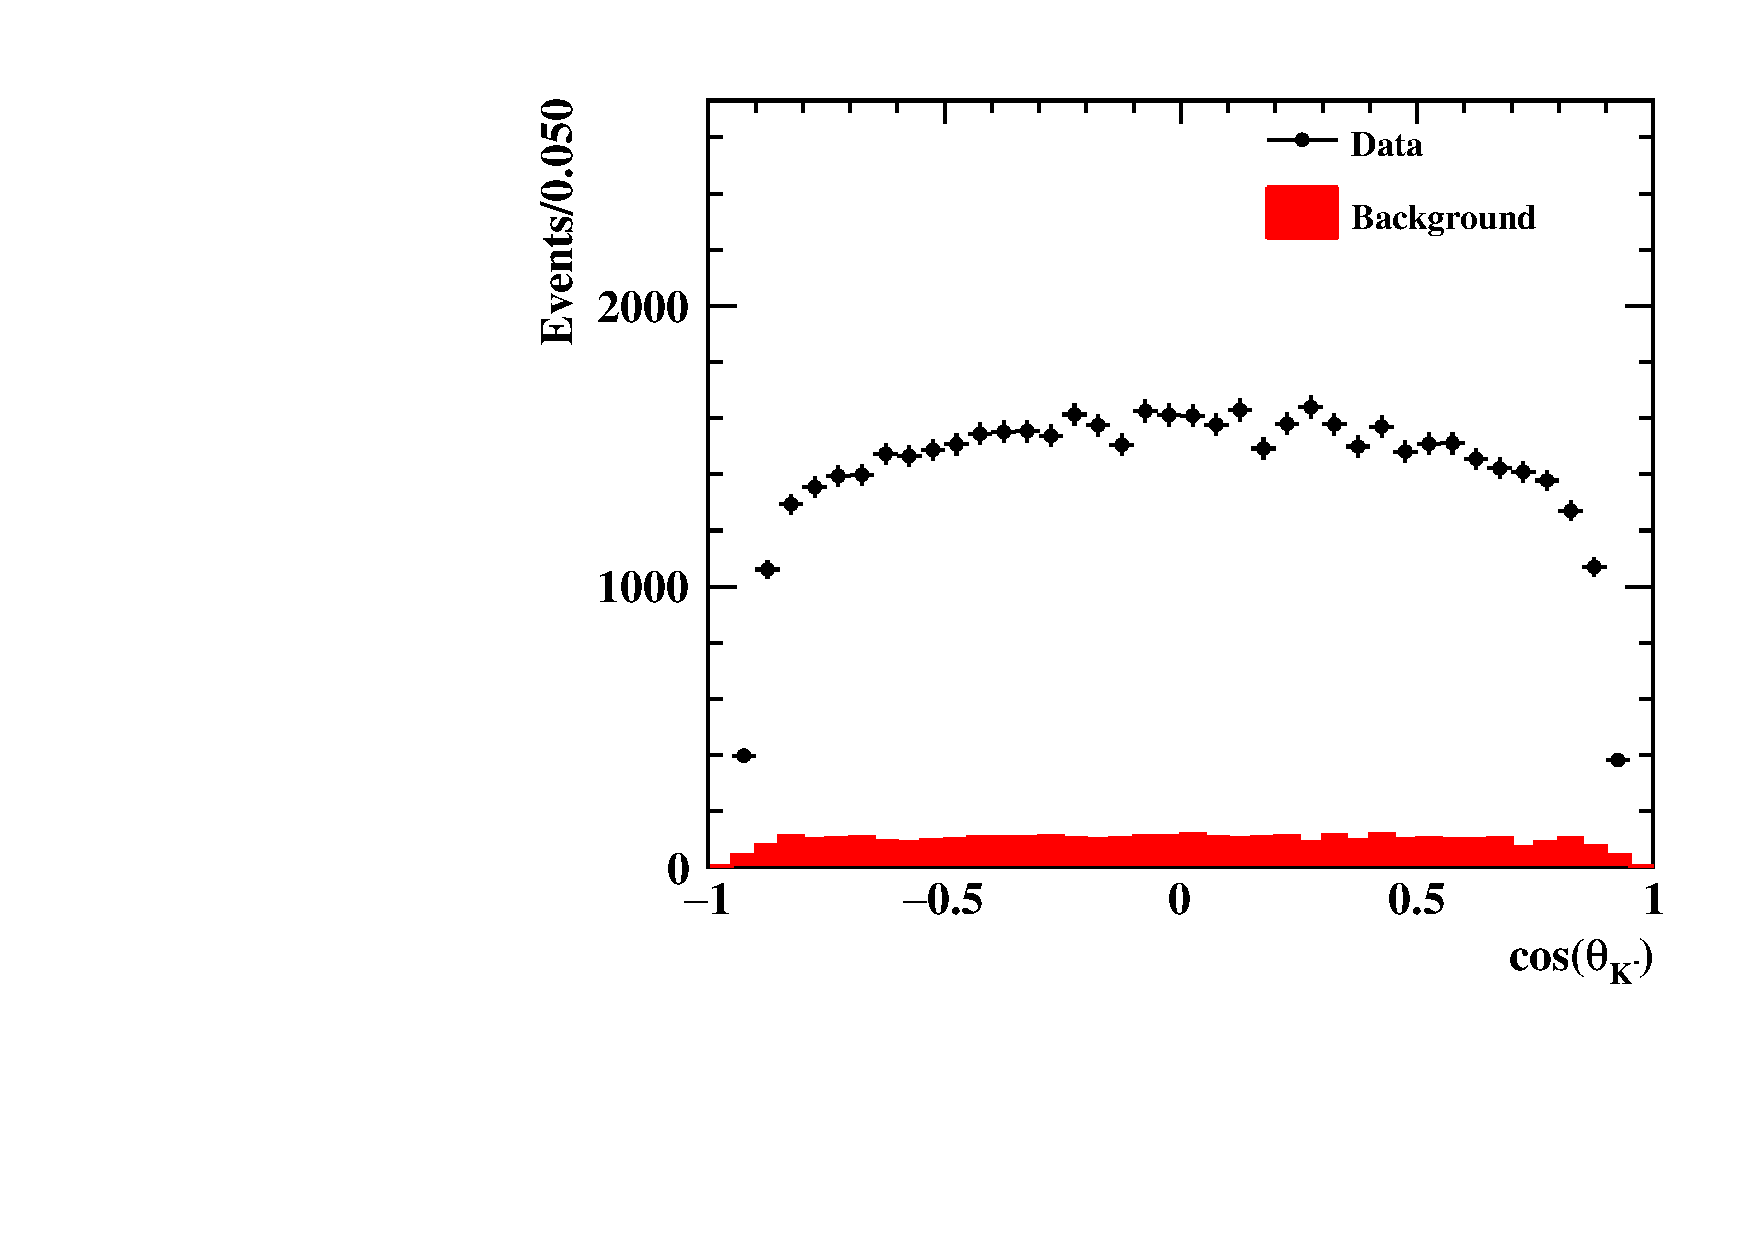
\includegraphics[width=0.32\textwidth]{figure/dalitz/output_data_mc_0_sideband_costheta2_1.pdf}
    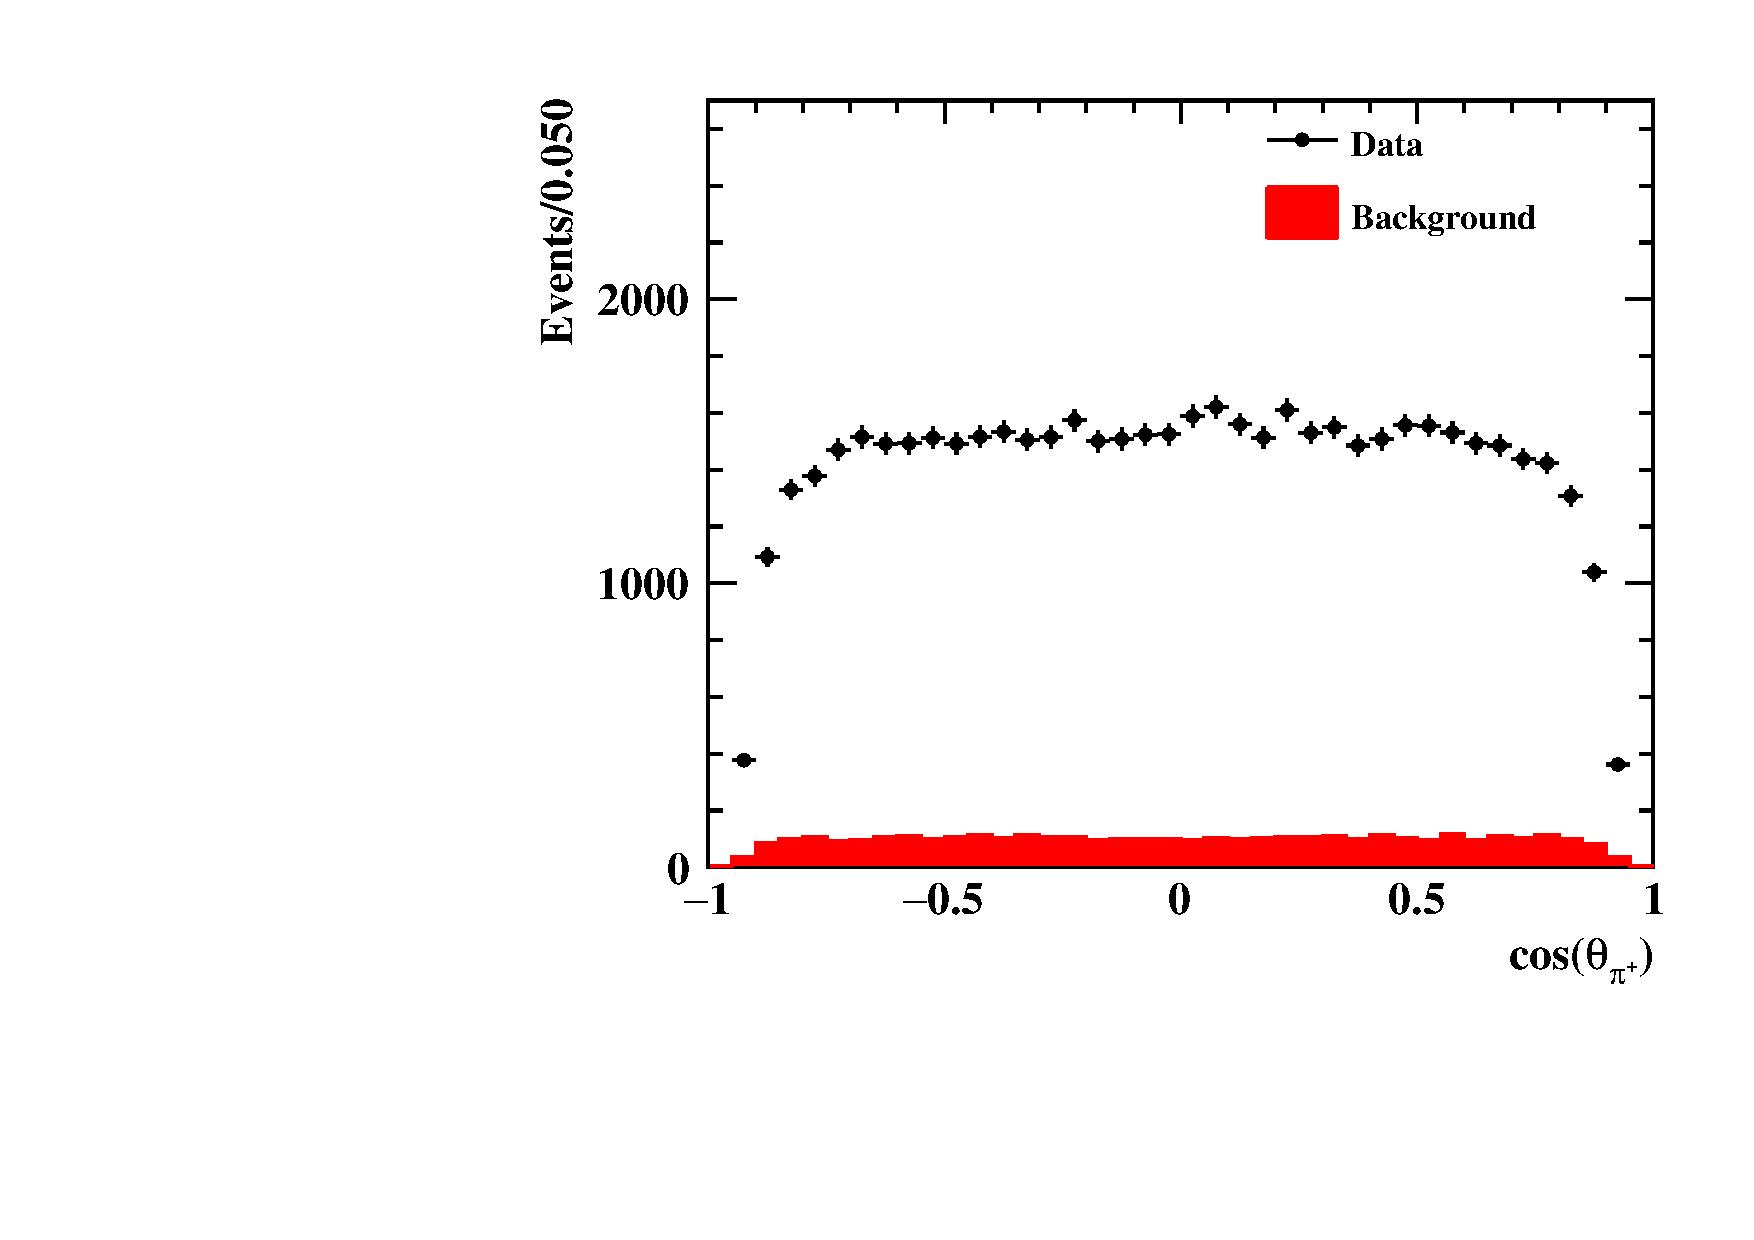
\includegraphics[width=0.32\textwidth]{figure/dalitz/output_data_mc_0_sideband_costheta3_1.pdf}
    \caption{Distributions of the squared two-body invariant mass and polar angles for the selected charged tracks.}
\label{fig:projected_plots}
\end{figure}

\subsection{Helicity amplitude}
\label{sec:helicity_amplitude}
In this analysis, the decay amplitude is constructed using the helicity amplitude formalism~\cite{Chung:186421,Richman:153636} and implemented based on the TF-PWA\footnote[1]{Source codes are available in \hyperlink{github}{https://github.com/jiangyi15/tf-pwa}} package. All final state particles are boosted to the c.m. frame of $e^+e^-$. Under the assumption of CP conservation, the parameters of $\lcm$ amplitudes are related to those of $\lcp$ by performing a parity transformation, where the momenta of $\lcm$ are reversed. 
%Given the assumption of CP conservation, the amplitude of $\lcm$ is the same as the one of $\lcp$ with corresponding parameters performed by the parity transformation.
For process of $e^+e^- \to \gamma^* \to \lcp\lcm$ with $\lcp \to pK^-\pi^+$, its full decay amplitude is formed by the following three decay chains:
\begin{itemize}
    \item $e^+e^- \to \gamma^* \to \lcp\lcm$, $\lcp \to \Lambda^*\pi^+$, $\Lambda^* \to pK^-$, 
    \item $e^+e^- \to \gamma^* \to \lcp\lcm$, $\lcp \to \Delta^{++}K^-$, $\Delta^{++} \to p\pi^+$,
    \item $e^+e^- \to \gamma^* \to \lcp\lcm$, $\lcp \to p\overline{K}^*$, $\overline{K}^* \to K^-\pi^+$.
\end{itemize}
We consider the contributions from $\Lambda^*$, $\Delta^{++}$ and $\overline{K}^*$ resonances according to the PDG~\cite{Workman:2022ynf}. The contribution from $\Sigma^*\to pK^-$ is possible but expected to be suppressed due to the isospin difference of $\Delta I = 1$. It is also hard to separate the contributions between $\Lambda*$ and $\Sigma^*$. In Ref~\cite{LHCb:2022ouv}, the nominal results of amplitude analysis of $\lcp \to p K^-\pi^+$ showed that the dominant contributions were from the $\Lambda^*$ resonances. The $\Sigma^*$ ones were neglected and considered as part of systematic uncertainties. We follow the same strategy and the largest significant $\Sigma^*$ resonances are test and shown in Section~\ref{sec:syst_component}.
%We decide to neglect $\Sigma^*$, which was also done in Ref.~\cite{LHCb:2022ouv}.

The helicity formalism is constructed based on the Isobar model~\cite{Walker:1968xu}, which describes the three-body decay as sequential quasi-two-body decay. For each two body decay $0 \to 1 + 2$, the helicity amplitude can be written as
\begin{equation}\label{eq:2_body_helicity}
    A^{0 \rightarrow 1+2}_{\lambda_{0},\lambda_{1},\lambda_{2}} = H_{\lambda_{1},\lambda_{2}}^{0 \rightarrow 1+2} D^{J_{0}\ast}_{\lambda_{0},\lambda_{1}-\lambda_{2}}(\phi,\theta,0),
\end{equation}
where $H_{\lambda_{1},\lambda_{2}}^{0 \rightarrow 1+2}$ is the helicity coupling and can be expanded using LS coupling formula~\cite{PhysRevD.56.4419,PhysRevD.57.431} to
\begin{equation}
    H_{\lambda_{1},\lambda_{2}}^{0 \rightarrow 1+2} =
\sum_{ls} g_{ls} \sqrt{\frac{2l+1}{2 J_{0}+1}} \langle l0, s\delta|J_{0},\delta\rangle \langle J_{1} J_{2}, \lambda_{1} -\lambda_{2} | s, \delta \rangle \left(\frac{q}{q_0}\right)^l B_{l}'(q, q_0, d), 
\end{equation}
where $g_{ls}$ is the partial wave amplitude, $J_{0,1,2}$ are the spins for particle 0, 1 and 2, $\lambda_{1,2}$ are the helicity for particle 1 and 2, and the $\delta = \lambda_1 - \lambda_2$ is the difference of helicity. $q$ is the momentum of particle 1 in the rest frame of particle 0, which can be written as
\begin{equation}
    q = \frac{\sqrt{[m^2 - (m_1+m_2)^2][m^2 - (m_1 - m_2)^2]}}{2m},
\end{equation}
where $m$, $m_1$ and $m_2$ are the invariant mass of two-body system of particle 1 and 2, the nominal mass values of particle 1 and 2, respectively. $q_0$ is the normalization factor calculated from $q$ with $m$ at resonance nominal mass value. $B_{l}'(q, q_0, d)$ is the reduced Baltt-Weisskopf barrier factor~\cite{Blatt:1952ije}, which is explicitly expressed as
\begin{equation}\label{eq:barrier_factor}
    \begin{split}
    B_{0}'(q, q_0, d) &= 1, \\
    B_{1}'(q, q_0, d) &= \sqrt{\frac{1+(q_0d)^2}{1+(qd)^2}}, \\
    B_{2}'(q, q_0, d) &= \sqrt{\frac{9+3(q_0d)^2+(q_0d)^4}{9+3(qd)^2+(qd)^4}}, \\
    B_{3}'(q, q_0, d) &= \sqrt{\frac{225+45(q_0d)^2+6(q_0d)^4+(q_0d)^6}{225+45(qd)^2+6(qd)^4+(qd)^6}}, \\
    B_{4}'(q, q_0, d) &= \sqrt{\frac{11025+1575(q_0d)^2+135(q_0d)^4+10(q_0d)^6+(q_0d)^8}{11025+1575(qd)^2+135(qd)^4+10(qd)^6+(qd)^8}}
    \end{split}
\end{equation}
$D^{J_{0}\ast}_{\lambda_{0},\lambda_{1}-\lambda_{2}}(\phi,\theta,0)$ is Wigner D-function, where $\theta$ indicates the helicity angle of the decay of resonance and $\phi$ is defined as helicity angle between the decay plane of daughter particle and the one of its mother particle. More details about the definitions of helicity angles can be found in Ref~\cite{Wang:2020giv}. In Eq.~(\ref{eq:barrier_factor}), the radius of centrifugal barrier $d$ is chosen as $d=1/q_r=3.69(\rm{GeV}/c)^{-1}$, which is the same as in Ref.~\cite{BESIII:2019dme}.

The full amplitude of each component is the production of every two-body decay amplitudes and the dynamical part. For the $\Lambda^*(pK^-)$ resonances:   
\begin{equation}
    A_{\lambda_{\gamma^*},\lambda_{\bar{\Lambda}_c^{-}},\lambda_p}^{\Lambda^*} = \sum_{\lambda_{\Lambda_c^+},\lambda_{\Lambda^*}}A_{\lambda_{\gamma^*},\lambda_{\Lambda_c^+},\lambda_{\bar{\Lambda}_c^-}}^{\gamma^* \to \Lambda_c^+\bar{\Lambda}_c^-}A_{\lambda_{\Lambda_c^+},\lambda_{\Lambda^*},0}^{\Lambda_c^+\to\Lambda^*\pi^+}R_{\Lambda^*}(M_{pK^-})A_{\lambda_{\Lambda^*},\lambda_p,0}^{\Lambda^*\to pK^-}.
\end{equation}
For the $\Delta^{++}(p\pi^+)$ resonances: 
\begin{equation}
    A_{\lambda_{\gamma^*},\lambda_{\bar{\Lambda}_c^{-}},\lambda_p}^{\Delta^{++}} = \sum_{\lambda_{\Lambda_c^+},\lambda_{\Delta^{++}}}A_{\lambda_{\gamma^*},\lambda_{\Lambda_c^+},\lambda_{\bar{\Lambda}_c^-}}^{\gamma^* \to \Lambda_c^+\bar{\Lambda}_c^-}A_{\lambda_{\Lambda_c^+},\lambda_{\Delta^{++}},0}^{\Lambda_c^+\to\Delta^{++}K^-}R_{\Delta^{++}}(M_{p\pi^+})A_{\lambda_{\Delta^{++}},\lambda_p,0}^{\Delta^{++}\to p\pi^+}.
\end{equation}
For the $\overline{K}^*(K^-\pi^+)$ resonances:
\begin{equation}
    A_{\lambda_{\gamma^*},\lambda_{\bar{\Lambda}_c^{-}},\lambda_p}^{\overline{K}^{*0}} = \sum_{\lambda_{\Lambda_c^+},\lambda_{\overline{K}^{*0}}}A_{\lambda_{\gamma^*},\lambda_{\Lambda_c^+},\lambda_{\bar{\Lambda}_c^-}}^{\gamma^* \to \Lambda_c^+\bar{\Lambda}_c^-}A_{\lambda_{\Lambda_c^+},\lambda_{\overline{K}^{*0}},\lambda_p}^{\Lambda_c^+\to p \overline{K}^{*0}}R_{\overline{K}^{*0}}(M_{K^-\pi^+})A_{\lambda_{\overline{K}^{*0}},0,0}^{\overline{K}^{*0}\to K^-\pi^+}.
\end{equation}
The dynamic parts, $R_{\Lambda^*}(pK^-)$, $R_{\Delta^{++}}(p\pi^+)$ and $R_{\overline{K}^*}(K^-\pi^+)$, include different models and will be explained in Section~\ref{sec:resonances}.
The total amplitude is represented by summing all possible resonances as:
\begin{equation}\label{eq:total_amplitude}
    \begin{split}
    A_{\lambda_{\gamma^*},\lambda_{\bar{\Lambda}_c^{-}}, \lambda_p} &=  A_{\lambda_{\gamma^*},\lambda_{\bar{\Lambda}_c^{-}},\lambda_p}^{\Lambda^*} \\
    &+ \sum_{\lambda^{\prime}_{\bar{\Lambda}_c^-},\lambda^{\prime}_p}(\sum A_{\lambda_{\gamma^*},\lambda^{\prime}_{\bar{\Lambda}_c^{-}},\lambda^{\prime}_p}^{\Delta^{++}})D_{\lambda^{\prime}_{\bar{\Lambda}_c^-}, \lambda_{\bar{\Lambda}_c^-}}^{1/2}(\alpha_{\bar{\Lambda}_c^-}, \beta_{\bar{\Lambda}_c^-}, \gamma_{\bar{\Lambda}_c^-})D_{\lambda^{\prime}_{p}, \lambda_{p}}^{1/2}(\alpha_{p}, \beta_{p}, \gamma_{p})\\
    &+ \sum_{\lambda^{\prime}_{\bar{\Lambda}_c^-},\lambda^{\prime}_p}(\sum A_{\lambda_{\gamma^*},\lambda^{\prime}_{\bar{\Lambda}_c^{-}},\lambda^{\prime}_p}^{\overline{K}^*})D_{\lambda^{\prime}_{\bar{\Lambda}_c^-}, \lambda_{\bar{\Lambda}_c^-}}^{1/2}(\alpha^{\prime}_{\bar{\Lambda}_c^-}, \beta^{\prime}_{\bar{\Lambda}_c^-}, \gamma^{\prime}_{\bar{\Lambda}_c^-})D_{\lambda^{\prime}_{p}, \lambda_{p}}^{1/2}(\alpha^{\prime}_{p}, \beta^{\prime}_{p}, \gamma^{\prime}_{p}),
    \end{split}
\end{equation}
where the extra D-functions are added to align the final $\bar{\Lambda}_c^-$ and proton final states, correcting the helicities of $\bar{\Lambda}_c^-$ and proton in different chains. In the helicity amplitude Eq.~(\ref{eq:2_body_helicity}), the helicities of particle 1 and particle 2 are defined by the rotation ($\theta$, $\phi$) and boost sequences from initial states to final states. So it is necessary to include the extra D-functions in the sum of the amplitude within the same helicity. More details can be found in Ref.~\cite{BESIII:2022udq}.

\subsection{Resonance components and models}
\label{sec:resonances}
The full amplitude model is built by summing helicity amplitudes of all possible intermediate resonances, as indicated in Eq.~(\ref{eq:total_amplitude}). We consider the contributions from $\Lambda^*$, $\Delta^{++}$ and $\overline{K}^*$ and use the results in Ref.~\cite{LHCb:2022ouv} as starting point. The models and corresponding parameters are summarized in Table~\ref{tab:parameters}. The resolution effects are studied and documented in Appendix~\ref{app:resolution}.

\begin{table}[htbp]
    \centering
    \caption{List of $\Lambda^*$, $\Delta^{++}$ and $\overline{K}^*$ resonances considered in the amplitude model. The model parameters are taken according to the PDG~\cite{Workman:2022ynf} and LHCb's results\cite{LHCb:2022ouv}.}
    \label{tab:parameters}
    \begin{tabular}{ccccc}
        \hline\hline
        Resonance & $J^P$ & Mass (MeV)  & Width (MeV) & Model \\\hline
        $\Lambda(1405)$ & $1/2^-$ & 1405.1 & 50.5  & Flatte \\
        $\Lambda(1520)$ & $3/2^-$ & 1518.5 & 15.2  & Relativistic Breit-Wigner\\
        $\Lambda(1600)$ & $1/2^+$ & 1630   & 250   & Relativistic Breit-Wigner\\
        $\Lambda(1670)$ & $1/2^-$ & 1670   & 30    & Relativistic Breit-Wigner\\
        $\Lambda(1690)$ & $3/2^-$ & 1690   & 70    & Relativistic Breit-Wigner\\
        $\Lambda(2000)$ & $1/2^-$ & 1988   & 179   & Relativistic Breit-Wigner\\\hline
        $\Delta(1232)^{++}$ & $3/2^+$ & 1232 & 117 & Relativistic Breit-Wigner\\
        $\Delta(1600)^{++}$ & $3/2^+$ & 1640 & 300 & Relativistic Breit-Wigner\\
        $\Delta(1620)^{++}$ & $1/2^-$ & 1610 & 130 & Relativistic Breit-Wigner\\ 
        $\Delta(1700)^{++}$ & $3/2^-$ & 1690 & 380 & Relativistic Breit-Wigner\\\hline 
        $\overline{K}^*_0(700)$  & $0^+$ & 824 & 478 & Bugg\\
        $\overline{K}^*(892)$    & $1^-$ & 895.5 & 47.3 & Relativistic Breit-Wigner\\
        $\overline{K}^*_0(1430)$ & $0^+$ & 1375  & 190  & Bugg\\ 
        \hline\hline
    \end{tabular}
\end{table}

By default the resonances are parameterized by relativistic Briet-Wigner formula:
\begin{equation}
    R(m) = \frac{1}{m_0^2 - m^2 - im_0\Gamma(m)},
\end{equation} 
where the mass dependent width is
\begin{equation}
    \label{eq:bw_width}
    \Gamma(m) = \Gamma_0\left(\frac{q}{q_0}\right)^{2l+1}\frac{m_0}{m}B_l^{\prime 2}(q,q_0,d).
\end{equation}

The spin-zero $\overline{K}^*$ resonances, $\overline{K}^*(700)$ and $\overline{K}^*(1430)$, are described by a parameterization presented in Ref.~\cite{Bugg:2005xx}, which is also called Bugg lineshape. It consists of a Briet-Wigner lineshape, where the mass dependent width is replaced by
\begin{equation}
    \Gamma(m) = \frac{m^2-s_A}{m_0^2 - s_A}\Gamma_0e^{-\gamma m^2},
\end{equation}
which features a singularity (Adler zero) at $s_A = m_K^2 - 0.5m_\pi^2$ and exponential form factor on the $K\pi$ width driven by the parameter $\gamma$. The $\gamma$ parameters are fixed at 0.94 GeV$^{-2}$ and 0.02 GeV$^{-2}$ for $\overline{K}^*(700)$ and $\overline{K}^*(1430)$ respectively, according to Ref.~\cite{LHCb:2022ouv}. Comparing to the original parameterization in Ref.~\cite{Bugg:2005xx}, the additional overall exponential form factor and the opening of $K\eta$, $K\eta^\prime$ decay channels are neglect in the fit.

The $\Lambda(1405)$ resonance has the pole mass below the $pK^-$ threshold, which is parameterized by a Flatt\'e lineshape~\cite{Flatte:1976xu}. This lineshape describe the opening of the $pK$ decay channel in addition to the $\Sigma\pi$ decay. It consists of a Breit-Wigner lineshape with total width being the sum of the widths associated to the two decay channels,
\begin{equation}
    \Gamma(m) = \Gamma_{pK}(m) + \Gamma_{\Sigma\pi}(m),
\end{equation}
where $\Gamma_{pK}(m)$ and $\Gamma_{\Sigma\pi}(m)$ are calculated by Eq.~(\ref{eq:bw_width}) with $q_0$ derived from the decay of $\Sigma\pi$. $\Gamma_0$ is fixed at the total width of $\Lambda(1405)$ resonance in both term in the fit.
%The detailed formula can be written as:
%\begin{equation}
%    R(m) = \frac{1}{m^2 - m_0^2 - i(g_1\rho_{K\pi}(m) + g_2\rho_{\Sigma\pi})}, 
%\end{equation}
%where $g_1$ and $g_2$ are the coupling constant of $\Lambda(1405)$ to $pK$ and $\Sigma\pi$ channels, $\rho_{pK}$ and $\rho_{\Sigma\pi}$ are the available phase space for the the channels with $\rho = q/m$. 
%Comparing to the relativistic Breit-Wigner lineshape, the total width of $\Lambda(1405)$ is the sum of the widths of the two decay channels,
%\begin{equation}
%    \Gamma(m) = \Gamma_{pK}(m) + \Gamma_{\Sigma\pi}(m).
%\end{equation}
 

\subsection{Likelihood function and construction}
\label{sec:likelihood}
Using the total amplitude in Eq.~(\ref{eq:total_amplitude}), the probability distribution is defined as
\begin{equation}
    P(p_j) = \frac{\varepsilon(p_j)|A(p_j)|^2R_4(p_j)}{\int\varepsilon(p_j)|A(p_j)|^2R_4(p_j)\mathrm{d}p_j}, \,\,|A|^2 = \sum_{\lambda_{\gamma^*},\lambda_{\bar{\Lambda}_c^-}, \lambda_p}|A_{\lambda_{\gamma^*},\lambda_{\bar{\Lambda}_c^-},\lambda_p}|^2,
\end{equation}
where $\varepsilon(p_j)$ is the detection efficiency as a function of four momentum ($p_j$) of final particles. The integration part in the denominator is calculated by the sum of the phase space MC mentioned in Section~\ref{sec:sample} 
\begin{equation}\label{eq:mc_integration}
    \int\varepsilon(p_j)|A(p_j)|^2R_4(p_j)\mathrm{d}p_j \varpropto \frac{1}{N_\mathrm{PHSP}}\sum_{i \in \mathrm{{PHSP}}} |A(x_i)|^2.
\end{equation}
The negative log likelihood (NLL) is formed using the background subtraction method:
\begin{equation}\label{eq:nll}
    -\ln L = -\alpha\left[\sum_{i\in\mathrm{data}}\ln P(x_i) - w^\prime_\mathrm{bkg}\sum_{j\in sideband} \ln P(x_j)\right],
\end{equation}
where the background extrapolation factor $w^{\prime}_\mathrm{bkg} = w_\mathrm{bkg} \cdot N_\mathrm{data}/N_\mathrm{sideband}$ and $w_\mathrm{bkg}$ is the background fraction within $\mbc$ signal reigon obtained from the fit on $\mbc$. The normalization factor $\alpha$~\cite{Langenbruch_2022} is defined as 
%The normalization factor~\cite{Langenbruch_2022} used to correct errors is expressed as
\begin{equation}
    \alpha = \frac{N_\mathrm{data} - N_\mathrm{sideband}w^{\prime}_\mathrm{bkg}}{N_\mathrm{data} + N_\mathrm{sideband}w^{\prime 2}_\mathrm{bkg}}.
\end{equation}
It is used to include the effect of weights in the determination of uncertainties. Without considering it, uncertainties calculation will be underestimated.
The NLLs are created for each energy points with shared parameters arising from the decays of $\lcp$ and resonance states and separated partial wave amplitudes $g_{ls}$ in the process of $e^+e^-\to\gamma^*\to \lcp\lcm$. The joint NLL is obtained by summing all NLLs from each energy points. 

After minimizing the joint NLL, the parameters error matrix is calculated by the inverse hessian matrix:
\begin{equation}\label{eq:ff}
    V_{ij}^{-1} = - \frac{\partial^2 \ln L}{\partial \theta_i \partial \theta_j},
\end{equation}
where $\theta_i$ is the $i$-th floated parameters in the likelihood formula. This is the standard form of the error matrix in the maximum likelihood fit.

The fit fraction (FF) of each resonance state is calculated using
\begin{equation} \label{eq:ff2}
    \mathrm{FF}_{i} = \frac{\int |A_i|^2\mathrm{d}\Phi}{\int |\sum_k A_k|^2\mathrm{d}\Phi} \varpropto \frac{\sum_{j\in\mathrm{PHSP}}|A_i(x_j)|^2}{\sum_{j\in\mathrm{PHSP}}|\sum_k A_k(x_j)|^2},
\end{equation}
where $A_i$ is the amplitude of $i$-th component and the integration is calculated by summing the truth level PHSP MC samples without considering the detector response. The interference part between $i$-th and $j$-th components is derived by
\begin{equation}\label{eq:ff3}
    \mathrm{FF}_{i,j} = \frac{\int |A_i + A_j|^2\mathrm{d}\Phi}{\int |\sum_k A_k|^2\mathrm{d}\Phi} - \mathrm{FF}_i - \mathrm{FF}_j.
\end{equation}
The statistical uncertainties for FF are obtained with the standard form of error propagation. Let \textbf{\emph{Y}} be the variable whose error needs to be calculated, \textbf{\emph{X}} be the variables with a corresponding error matrix $V_{ij}$ in Eq.~(\ref{eq:ff}) and $\boldsymbol{\mu}$ be the nominal results of the floating variables \textbf{\emph{X}}, the variance of \textbf{\emph{Y}} is estimated as
\begin{equation}
    \sigma_Y^2 = \sum_{ij}\left(\frac{\partial Y}{\partial X_i}\right)_{\boldsymbol{X} = \boldsymbol{\mu}} V_{ij}\left(\frac{\partial Y}{\partial X_j}\right)_{\boldsymbol{X}=\boldsymbol{\mu}}.
\end{equation}
A validation test is performed using high-dimensional sampling considering the error matrix and details are documented in Appendix~\ref{app:ff_error}.

\subsection{Nominal fit results}
\label{sec:nominal_fit}
As a starting point, we use the nominal choice of resonances and fix their parameters as benchmark model based on Ref.~\cite{LHCb:2022ouv}. The statistical significance test is performed for additional $\Lambda^*$, $\Sigma^*$ and $\Delta^{++}$ resonance states, including $\Lambda(1800)$, $\Lambda(1810)$, $\Lambda(1820)$, $\Lambda(1830)$, $\Lambda(1890)$, $\Sigma(1670)$, $\Sigma(1750)$, $\Sigma(1775)$, $\Sigma(1915)$ and $\Delta(1620)^{++}$ with certain experimental evidence for resonance existence in the PDG~\cite{Workman:2022ynf}.
%with a score of at least three stars in PDG~\cite{Workman:2022ynf}. 
The statistical significance is calculated using the change of the NLL values with and without each additional resonance, by taking into account the change of the number of degree of freedom (NDF). The results show that $\Delta(1620)^{++}$ has a large significance with 5.7$\sigma$, while all the other components have significance values below 5$\sigma$. The additional resonances will be considered in the systematic uncertainties of model components in Section~\ref{sec:syst_component}. 
The final components of the nominal model and corresponding parameters are shown in Table~\ref{tab:parameters}. The statistical significance of each component is checked by comparing the fit results of the nominal model and the alternative one without the specific resonance. The significance is determined using the differences of NLL and NDF, summarized in Table~\ref{tab:nom_significance}. The constructed joint NLL includes 80 floated parameters, including (54) shared amplitudes and (26) separated partial wave amplitude $g_{ls}^{\gamma^*}$. The shared parameters are $g_{ls}$ of the decay of $\lcp \to Rh$ and $R$, where $R$ is the intermediate resonance and $h$ is the remaining final particle. They are expected to be identical in all 13 energy points. The fit quality is measured by a $\chi^2$ test performed over a 5-dimensional binning of phase space, which describe the amplitude of $\lcp\to p K^-\pi^+$. The selected variables are two Dalitz variables ($M^2(pK^-)$, $M^2(K^-\pi^+)$) and three helicity angles ($\phi_{p}^{\lcp}$, $\cos(\theta_{p})$ and $\phi_{K^{-}}^{\bar{K^{*}}}$), where $\phi_{p}^{\lcp}$ is the angle between the plane made by $p$ and $\bar{K}^*$ and $\lcp$ production plane, $\cos(\theta_{p})$ is the angle between the momenta of $p$ and $\lcp$ in the $\lcp$ rest frame, $\phi_{K^{-}}^{\bar{K^{*}}}$ is the angle between the planes made by $K^-\pi^+$ and $p \bar{K}^*$. An adaptive binning technique is employed to guarantee similar number of data events in each bin. The projected invariant mass distributions and helicity angles are shown in Figure~\ref{fig:pwa_nominal_comb} combining all 13 energy points.

\begin{figure}[htbp]\centering
    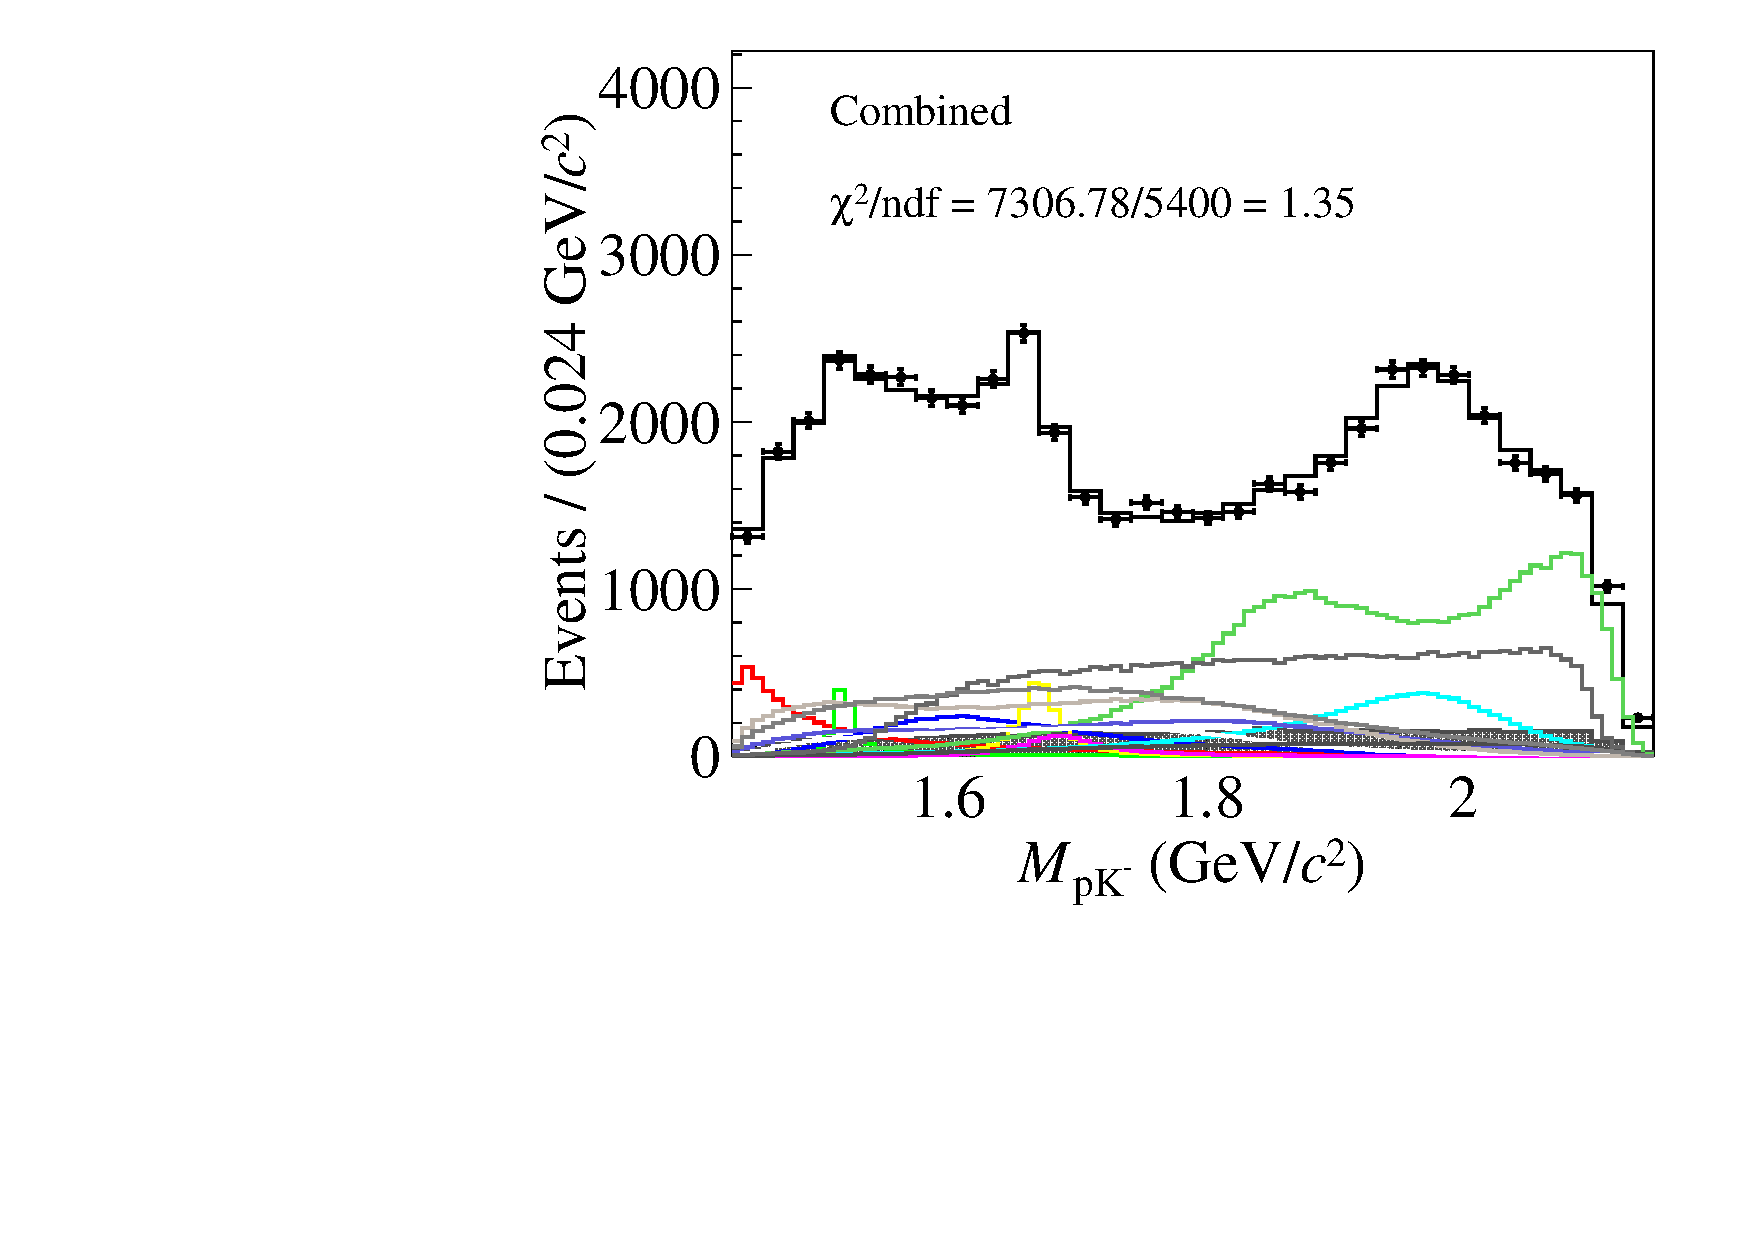
\includegraphics[width=0.32\textwidth]{figure/pwa_nominal/data_all_m_R_BC.pdf}
    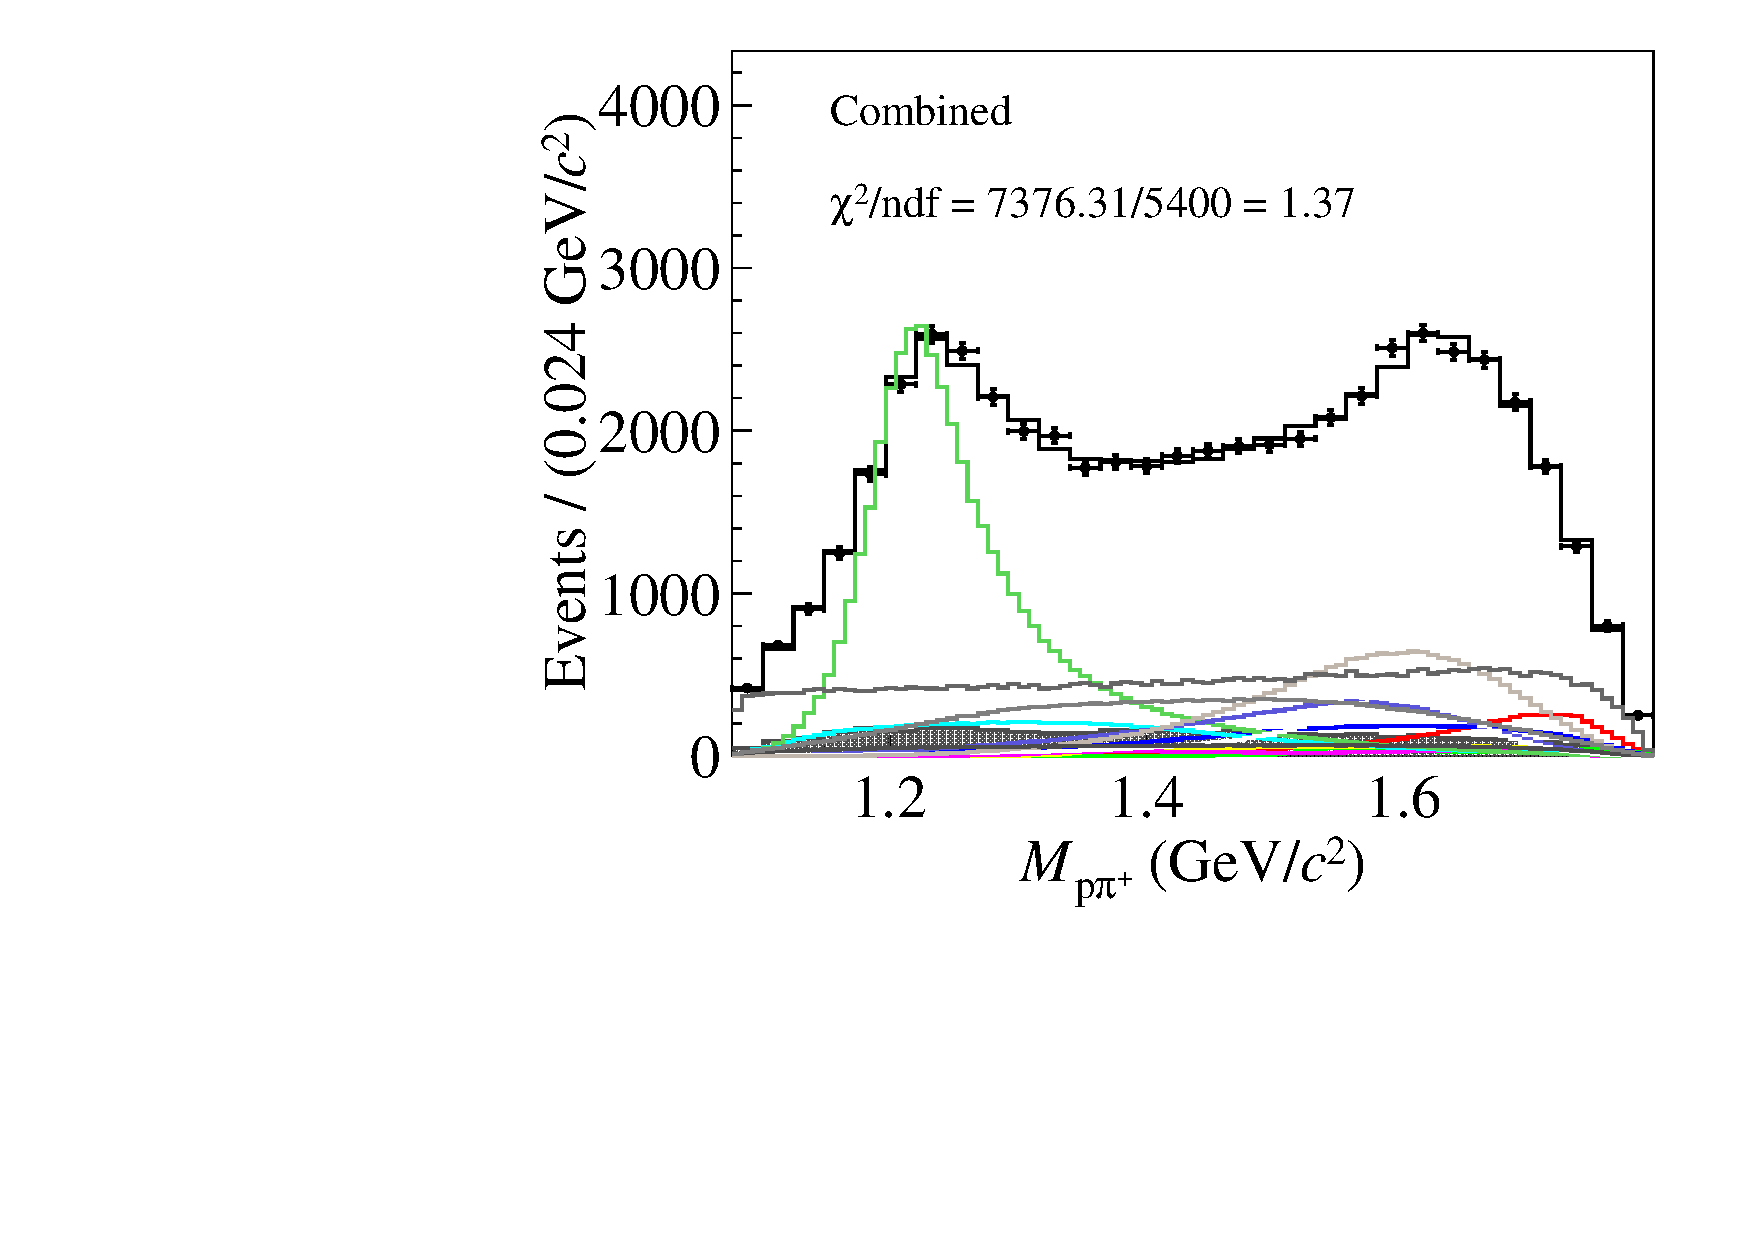
\includegraphics[width=0.32\textwidth]{figure/pwa_nominal/data_all_m_R_BD.pdf}
    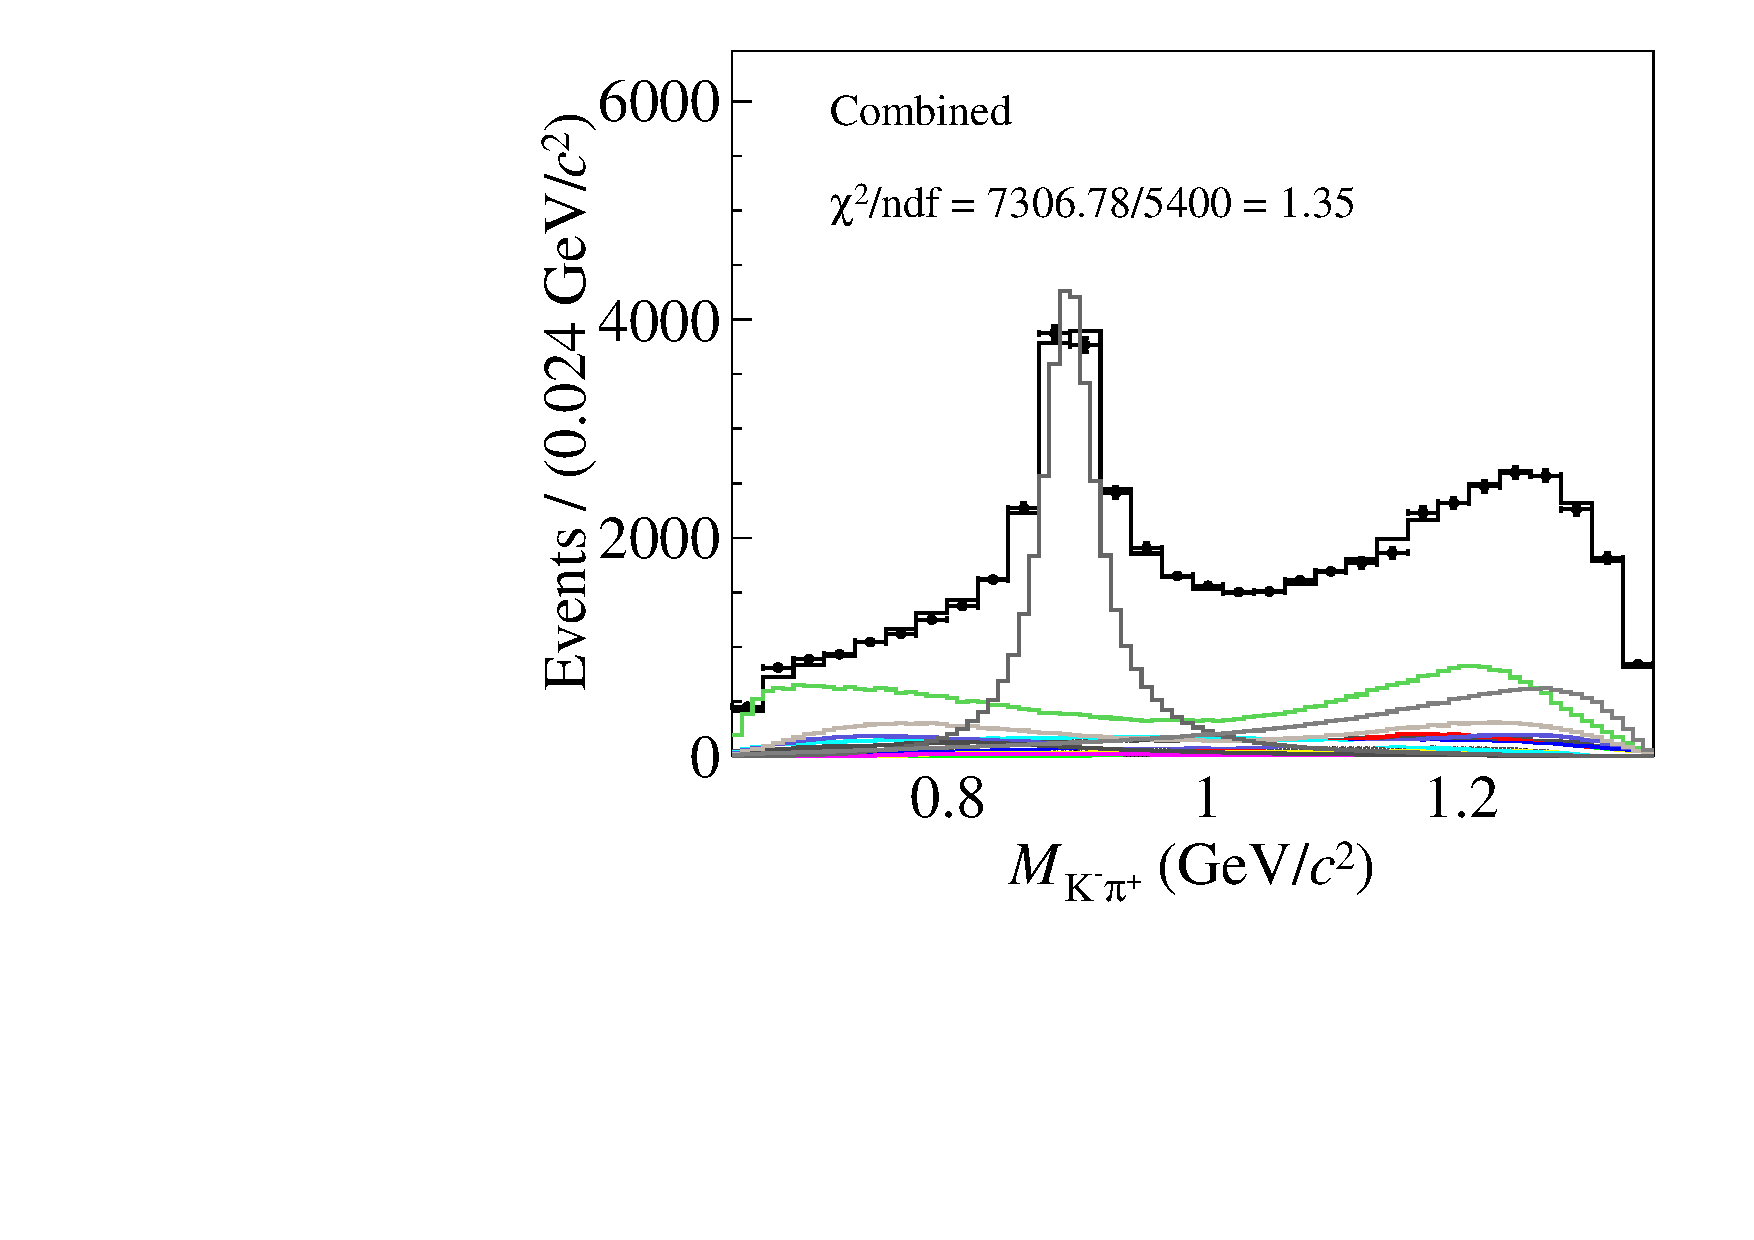
\includegraphics[width=0.32\textwidth]{figure/pwa_nominal/data_all_m_R_CD.pdf} \\
    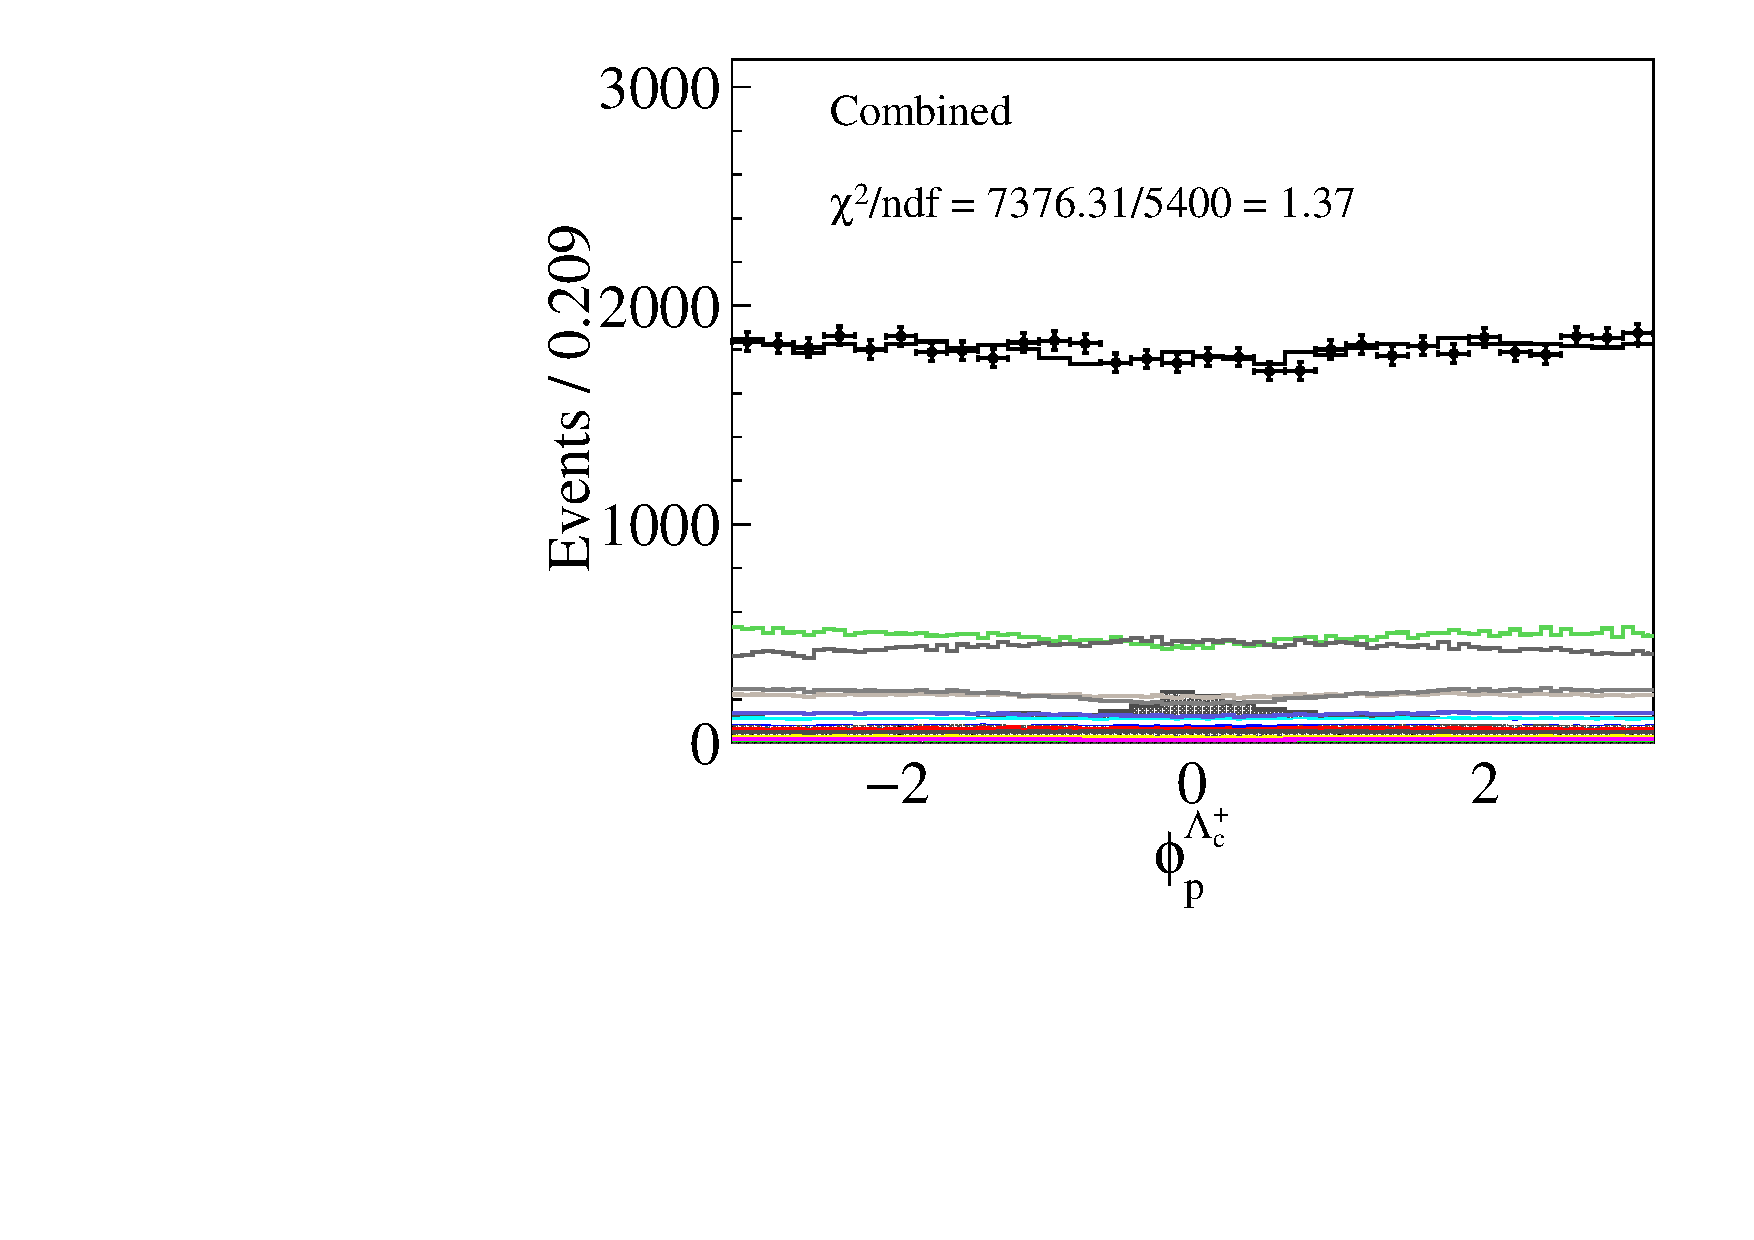
\includegraphics[width=0.32\textwidth]{figure/pwa_nominal/data_all_Lmdc_p_alpha.pdf}
    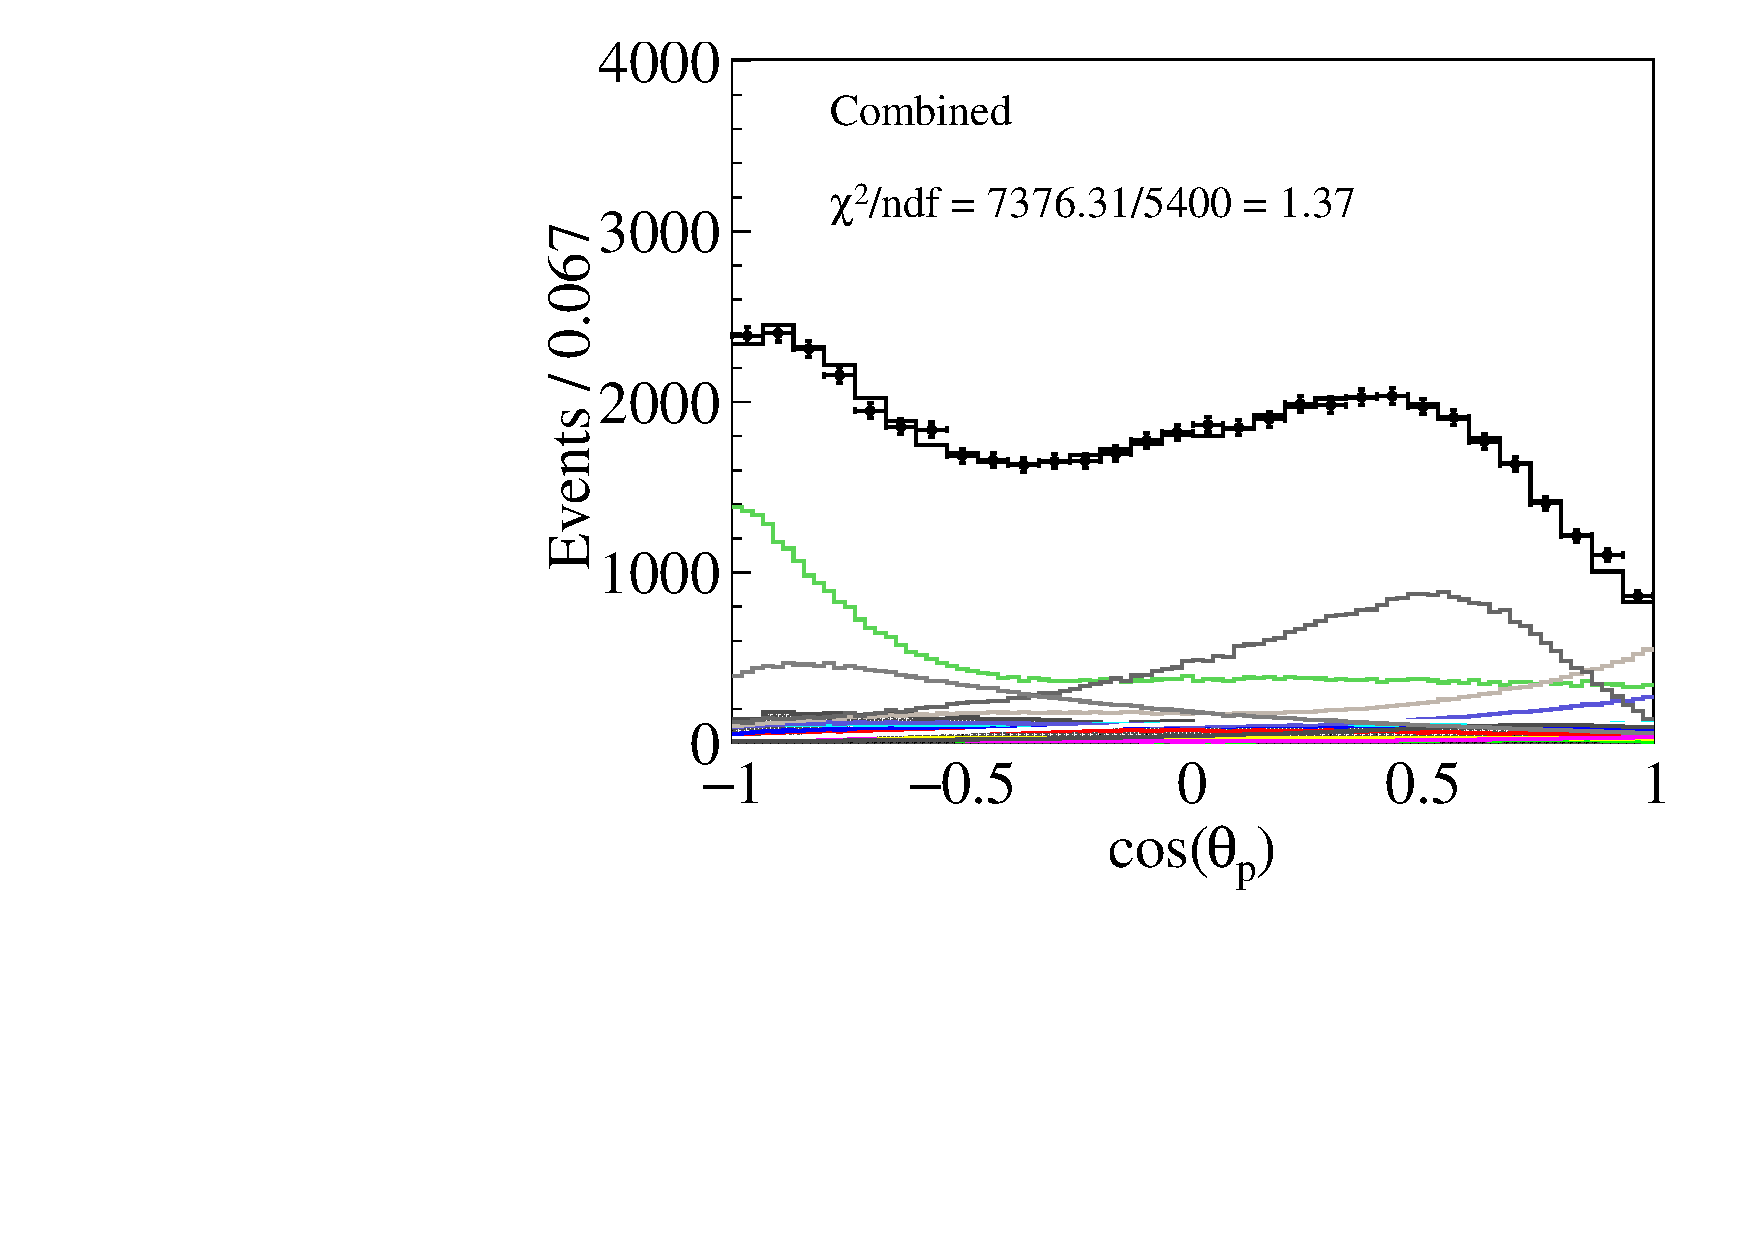
\includegraphics[width=0.32\textwidth]{figure/pwa_nominal/data_all_Lmdc_p_cos_beta.pdf}
    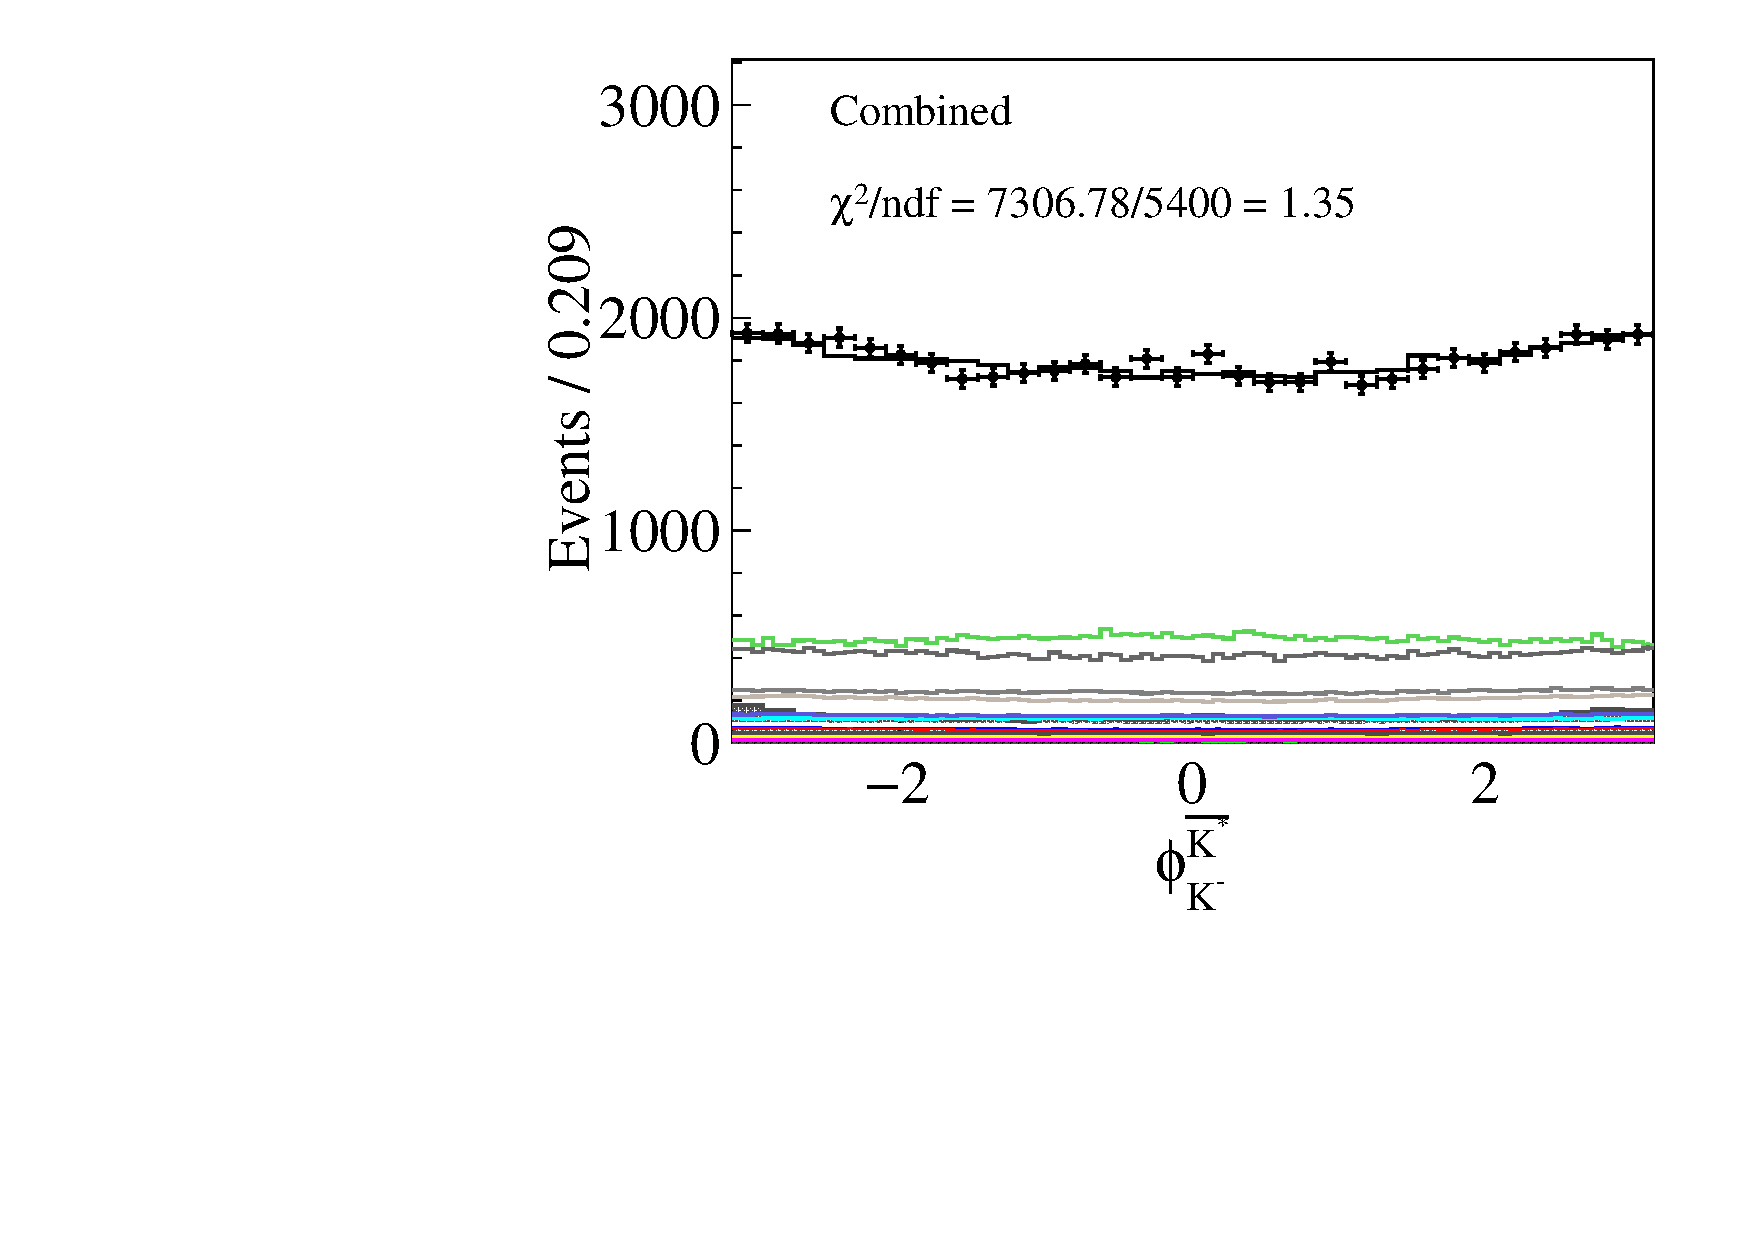
\includegraphics[width=0.32\textwidth]{figure/pwa_nominal/data_all_R_CD_k_alpha.pdf} \\
    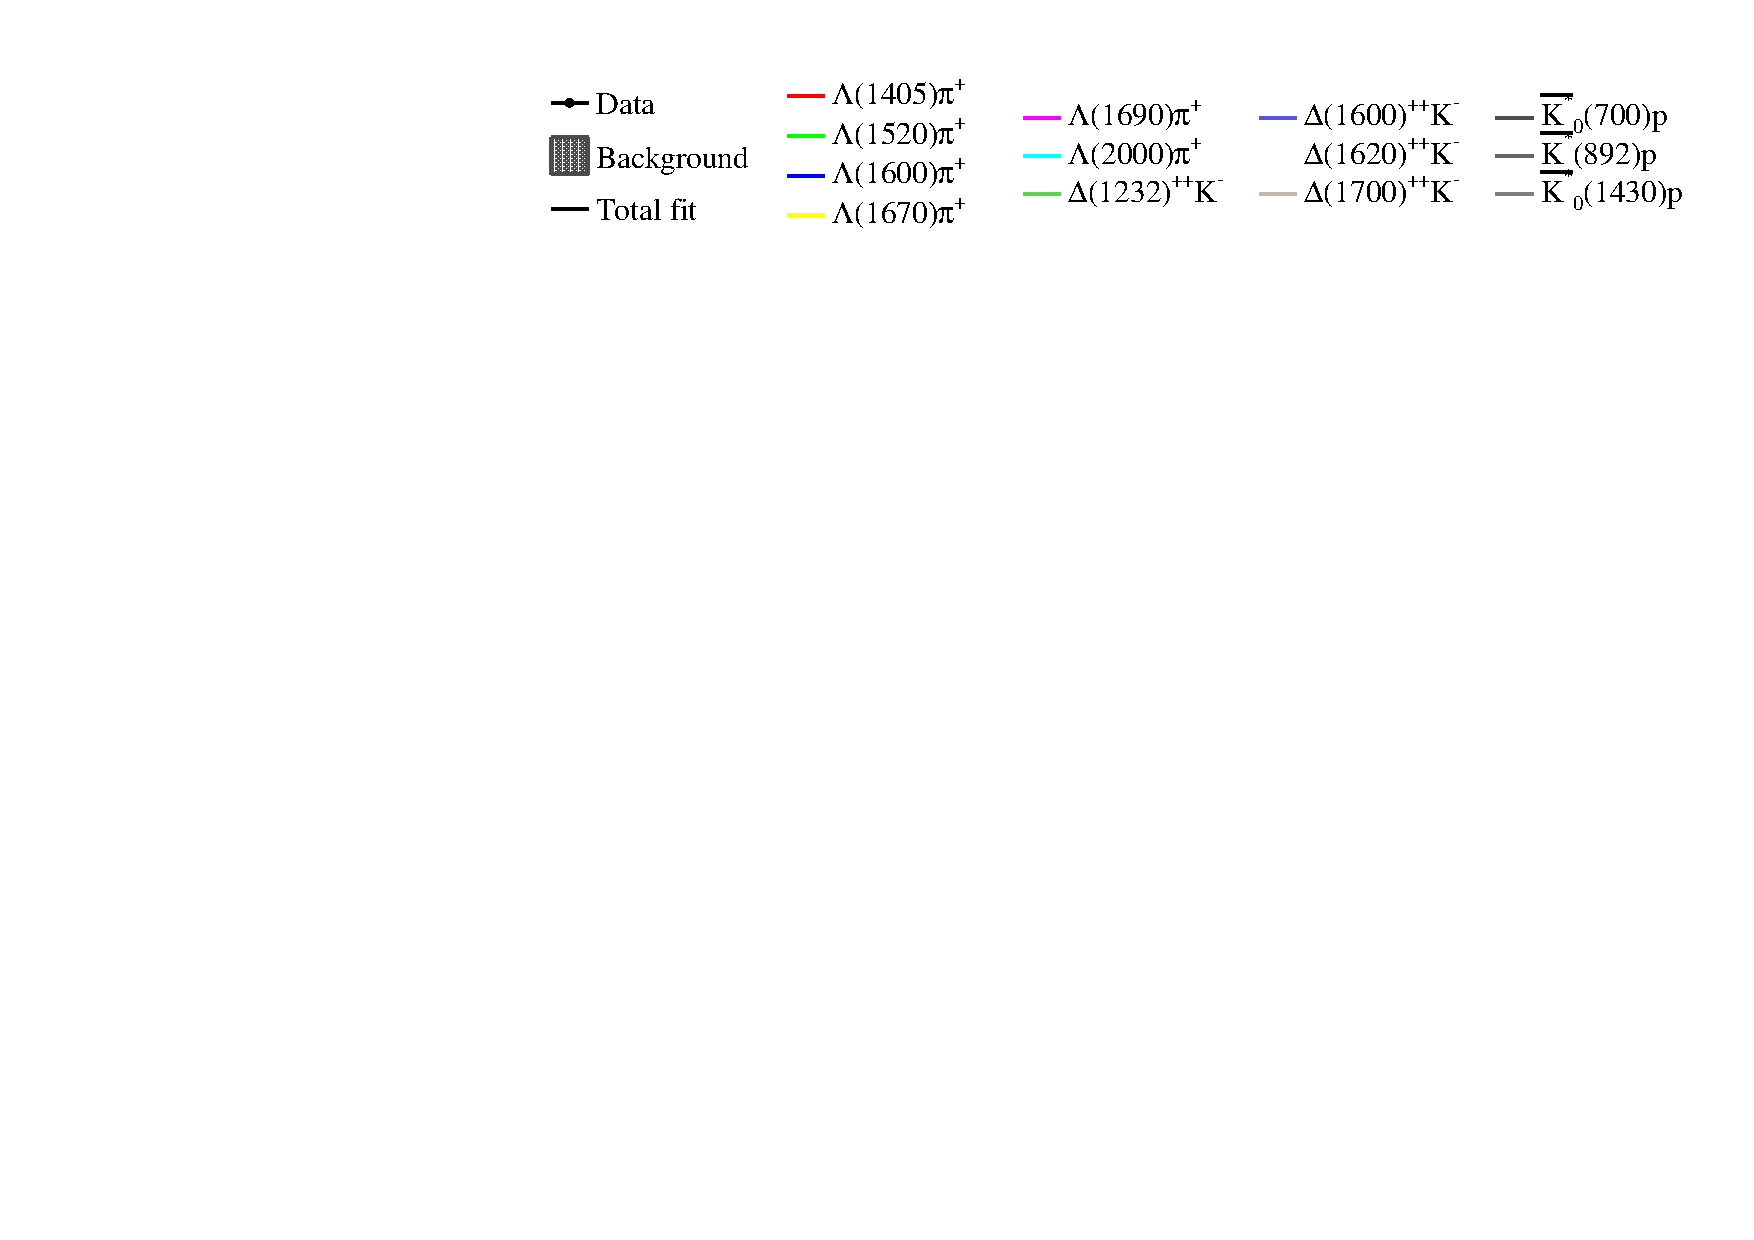
\includegraphics[width=0.80\textwidth]{figure/pwa_nominal/legend.pdf}

    \caption{Combined fit results of projected distributions of $M(pK^-)$, $M(p\pi^+)$, $M(K^-\pi^+)$ and helicity angle $\phi_{p}^{\lcp}$, $\cos(\theta_{p})$ and $\phi_{K^{-}}^{\bar{K^{*}}}$. }
\label{fig:pwa_nominal_comb}
\end{figure}

Figure~\ref{fig:pwa_fit_mass_0}-\ref{fig:pwa_fit_mass_1} show the projected two-body invariant mass and helicity angle of $\lcp$ distributions from the fit for each energy point. The fit fractions of each component and the interference part are shown in Table~\ref{tab:ff_s6} for $\sqrt{s} = 4.682\gev/c^2$. The total FF is 111.71$\pm$4.66\%. As the parameters of $\lcp$ decay are shared among all energy points, the fit fractions results are almost same with small difference due to the statistical fluctuations from the PHSP MC samples. Comparison of FF of each component at different energy points are listed in Table~\ref{tab:ff_full}.  The partial wave amplitudes ($g_{ls}^{\gamma^*}$) and derived $\alpha_0$ and $\Delta_0$ are shown in Table~\ref{tab:fit_polarization} for each energy point.

\begin{table}[h]
    \centering
    \caption{The difference for NLL and NDF between with and without each resonance state, the statistical significance values for each component in the nominal model.}
    \label{tab:nom_significance}
    \begin{tabular}{cccc}
        \hline\hline
    Resonance & $\Delta_{\rm NLL}$ & $\Delta_{\rm NDF}$ & Significance \\\hline
    $\Lambda(1405)$ & -103.29 & 4 & 13.8$\sigma$\\
    $\Lambda(1520)$ & -78.76 & 4 & 12.0$\sigma$\\
    $\Lambda(1600)$ & -26.37 & 4 & 6.5$\sigma$\\
    $\Lambda(1670)$ & -82.00 & 4 & 12.2$\sigma$\\
    $\Lambda(1690)$ & -24.61 & 4 & 6.2$\sigma$\\
    $\Lambda(2000)$ & -256.98 & 4 & 22.3$\sigma$\\
    $\Delta(1232)^{++}$ & -477.81 & 4 & 30.6$\sigma$\\
    $\Delta(1600)^{++}$ & -34.93 & 4 & 7.6$\sigma$\\
    $\Delta(1620)^{++}$ & -19.17 & 4 & 5.3$\sigma$\\
    $\Delta(1700)^{++}$ & -66.59 & 4 & 10.9$\sigma$\\
    $\bar{K}^{*}_{0}(700)$ & -31.11 & 4 & 7.1$\sigma$\\
    $\bar{K}^{*}(892)$ & -1281.70 & 8 & $>30\sigma$\\
    $\bar{K}^{*}_{0}(1430)$ & -70.74 & 4 & 11.3$\sigma$\\
    \hline\hline
    \end{tabular}
\end{table}

\begin{figure}[htbp]\centering
    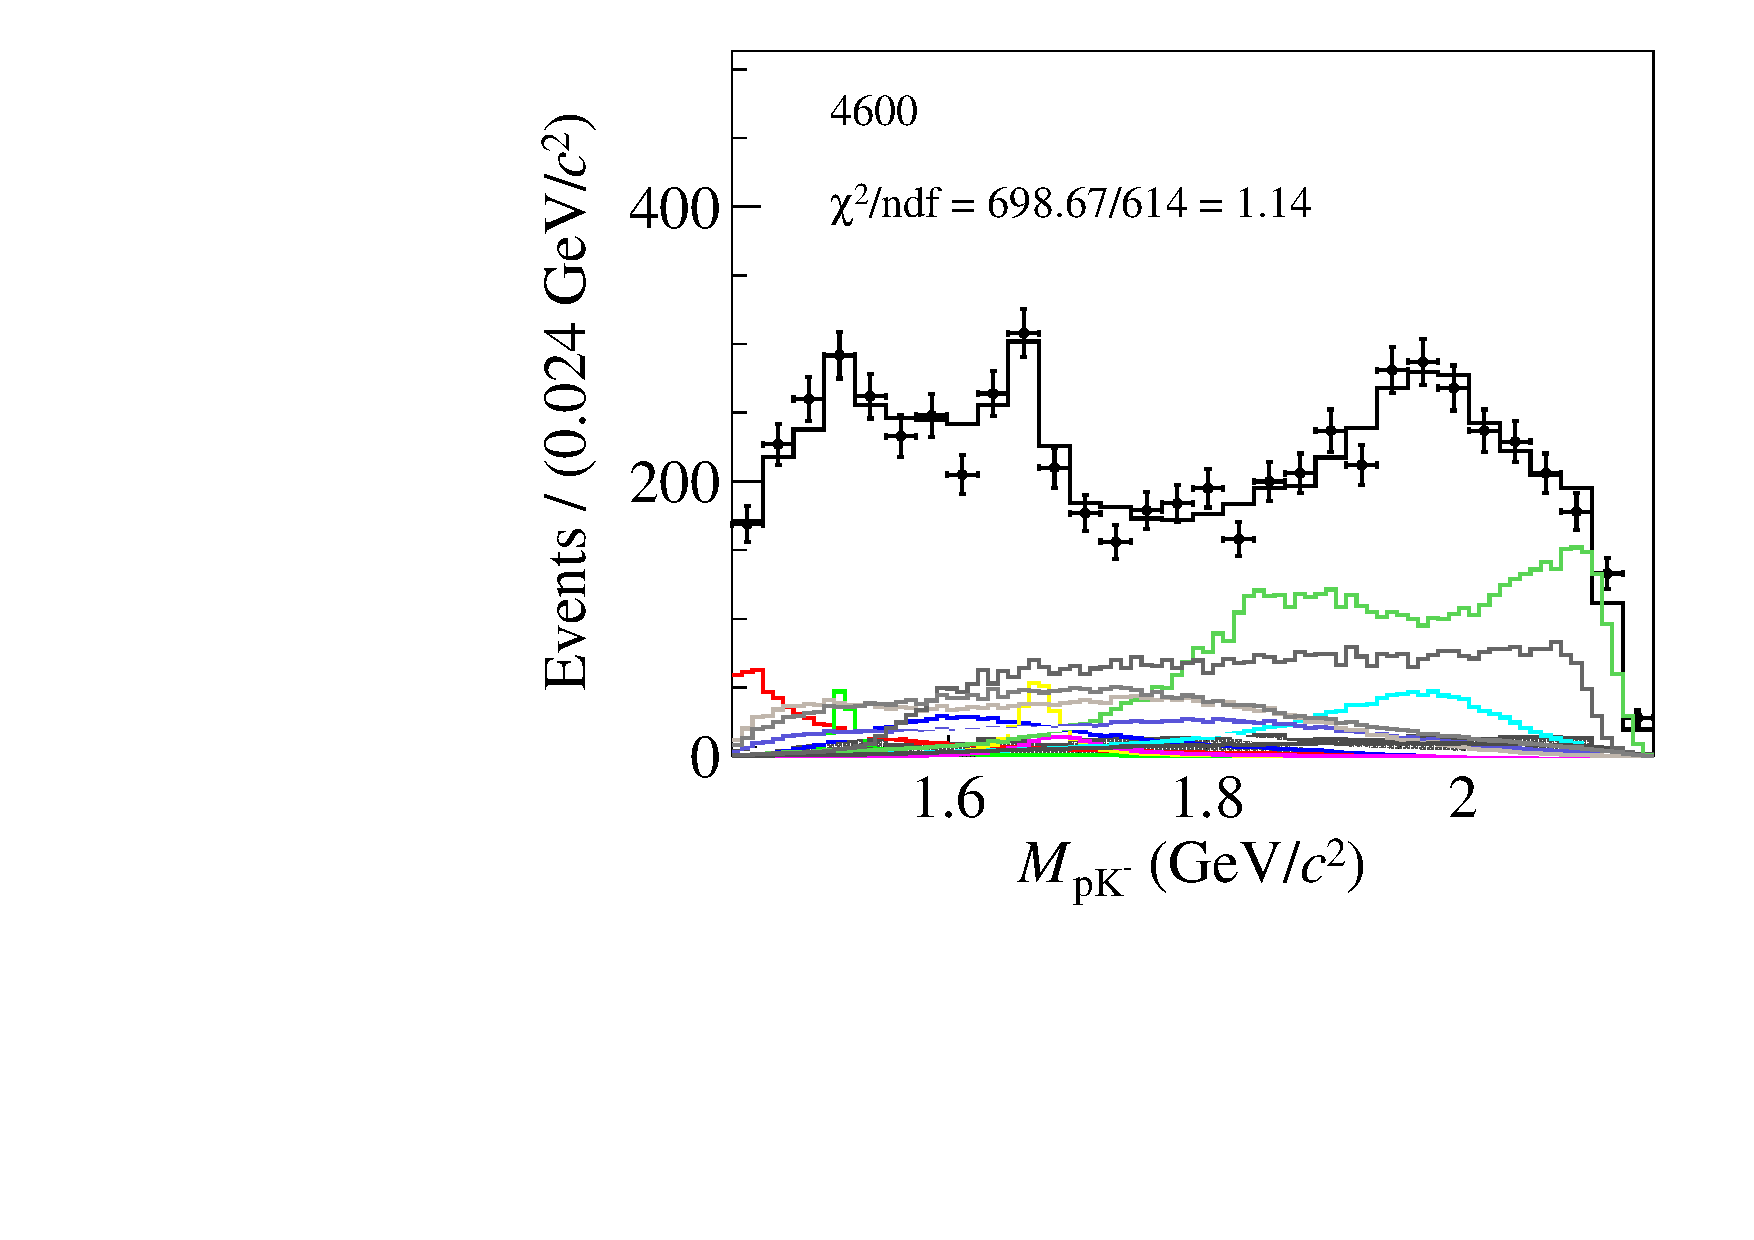
\includegraphics[width=0.24\textwidth]{figure/pwa_nominal/s0_m_R_BC.pdf}
    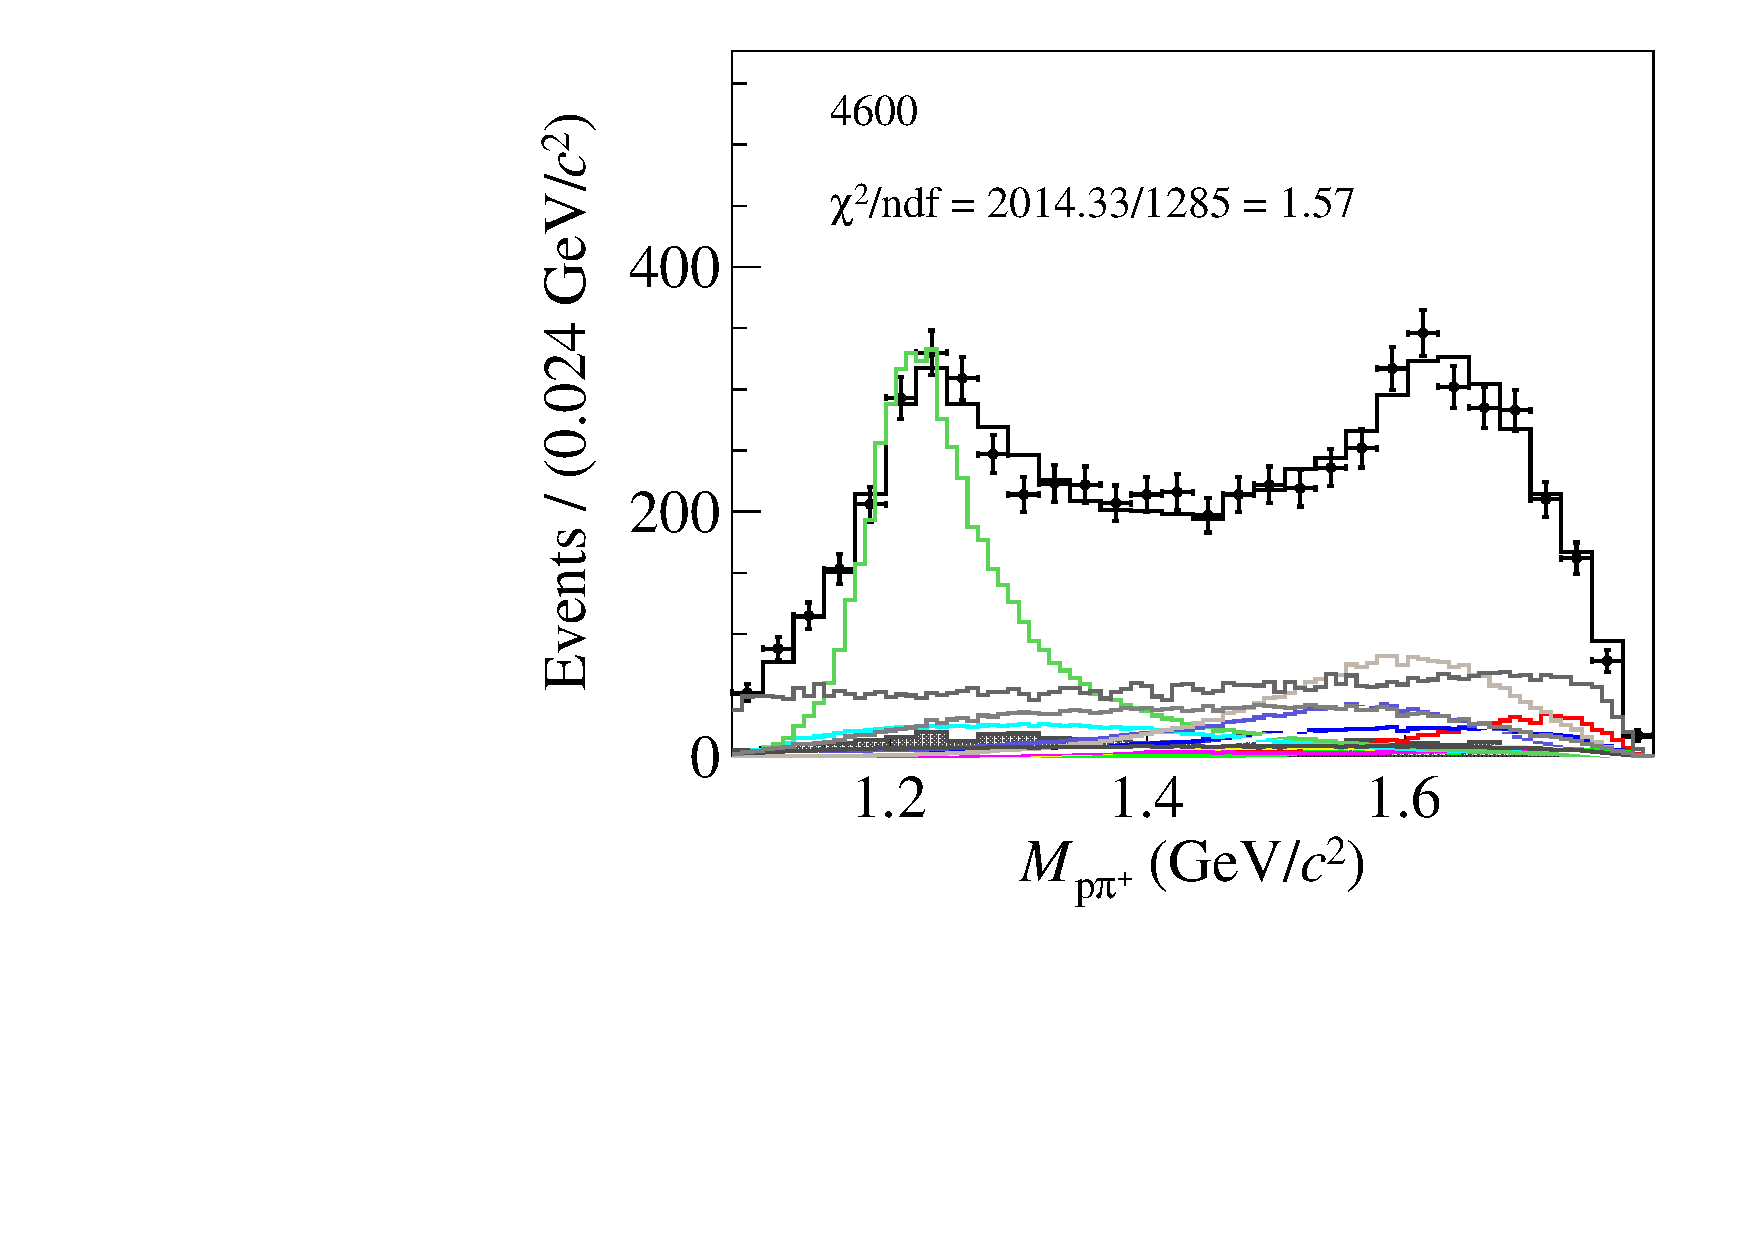
\includegraphics[width=0.24\textwidth]{figure/pwa_nominal/s0_m_R_BD.pdf}
    \includegraphics[width=0.24\textwidth]{figure/pwa_nominal/s0_m_R_CD.pdf}
    \includegraphics[width=0.24\textwidth]{figure/pwa_nominal/s0_epemDSID_Lmdc_cos_beta.pdf} \\
    \includegraphics[width=0.24\textwidth]{figure/pwa_nominal/s1_m_R_BC.pdf}
    \includegraphics[width=0.24\textwidth]{figure/pwa_nominal/s1_m_R_BD.pdf}
    \includegraphics[width=0.24\textwidth]{figure/pwa_nominal/s1_m_R_CD.pdf}
    \includegraphics[width=0.24\textwidth]{figure/pwa_nominal/s1_epemDSID_Lmdc_cos_beta.pdf} \\
    \includegraphics[width=0.24\textwidth]{figure/pwa_nominal/s2_m_R_BC.pdf}
    \includegraphics[width=0.24\textwidth]{figure/pwa_nominal/s2_m_R_BD.pdf}
    \includegraphics[width=0.24\textwidth]{figure/pwa_nominal/s2_m_R_CD.pdf}
    \includegraphics[width=0.24\textwidth]{figure/pwa_nominal/s2_epemDSID_Lmdc_cos_beta.pdf} \\
    \includegraphics[width=0.24\textwidth]{figure/pwa_nominal/s3_m_R_BC.pdf}
    \includegraphics[width=0.24\textwidth]{figure/pwa_nominal/s3_m_R_BD.pdf}
    \includegraphics[width=0.24\textwidth]{figure/pwa_nominal/s3_m_R_CD.pdf}
    \includegraphics[width=0.24\textwidth]{figure/pwa_nominal/s3_epemDSID_Lmdc_cos_beta.pdf} \\
    \includegraphics[width=0.24\textwidth]{figure/pwa_nominal/s4_m_R_BC.pdf}
    \includegraphics[width=0.24\textwidth]{figure/pwa_nominal/s4_m_R_BD.pdf}
    \includegraphics[width=0.24\textwidth]{figure/pwa_nominal/s4_m_R_CD.pdf}
    \includegraphics[width=0.24\textwidth]{figure/pwa_nominal/s4_epemDSID_Lmdc_cos_beta.pdf} \\
    \includegraphics[width=0.24\textwidth]{figure/pwa_nominal/s5_m_R_BC.pdf}
    \includegraphics[width=0.24\textwidth]{figure/pwa_nominal/s5_m_R_BD.pdf}
    \includegraphics[width=0.24\textwidth]{figure/pwa_nominal/s5_m_R_CD.pdf}
    \includegraphics[width=0.24\textwidth]{figure/pwa_nominal/s5_epemDSID_Lmdc_cos_beta.pdf} \\
    \includegraphics[width=0.24\textwidth]{figure/pwa_nominal/s6_m_R_BC.pdf}
    \includegraphics[width=0.24\textwidth]{figure/pwa_nominal/s6_m_R_BD.pdf}
    \includegraphics[width=0.24\textwidth]{figure/pwa_nominal/s6_m_R_CD.pdf}
    \includegraphics[width=0.24\textwidth]{figure/pwa_nominal/s6_epemDSID_Lmdc_cos_beta.pdf} \\
    \includegraphics[width=0.80\textwidth]{figure/pwa_nominal/legend.pdf}

    \caption{Fit results of projected distributions of $M(pK^-)$, $M(p\pi^+)$, $M(K^-\pi^+)$  and helicity angle $\cos(\theta_{\lcp}^{\gamma^*})$ for energy points below $\sqrt{s} = 4.740\gev/c^2$. }
\label{fig:pwa_fit_mass_0}
\end{figure}

\begin{figure}[htbp]\centering
    \includegraphics[width=0.24\textwidth]{figure/pwa_nominal/s7_m_R_BC.pdf}
    \includegraphics[width=0.24\textwidth]{figure/pwa_nominal/s7_m_R_BD.pdf}
    \includegraphics[width=0.24\textwidth]{figure/pwa_nominal/s7_m_R_CD.pdf}
    \includegraphics[width=0.24\textwidth]{figure/pwa_nominal/s7_epemDSID_Lmdc_cos_beta.pdf} \\
    \includegraphics[width=0.24\textwidth]{figure/pwa_nominal/s8_m_R_BC.pdf}
    \includegraphics[width=0.24\textwidth]{figure/pwa_nominal/s8_m_R_BD.pdf}
    \includegraphics[width=0.24\textwidth]{figure/pwa_nominal/s8_m_R_CD.pdf}
    \includegraphics[width=0.24\textwidth]{figure/pwa_nominal/s8_epemDSID_Lmdc_cos_beta.pdf} \\
    \includegraphics[width=0.24\textwidth]{figure/pwa_nominal/s9_m_R_BC.pdf}
    \includegraphics[width=0.24\textwidth]{figure/pwa_nominal/s9_m_R_BD.pdf}
    \includegraphics[width=0.24\textwidth]{figure/pwa_nominal/s9_m_R_CD.pdf}
    \includegraphics[width=0.24\textwidth]{figure/pwa_nominal/s9_epemDSID_Lmdc_cos_beta.pdf} \\
    \includegraphics[width=0.24\textwidth]{figure/pwa_nominal/s10_m_R_BC.pdf}
    \includegraphics[width=0.24\textwidth]{figure/pwa_nominal/s10_m_R_BD.pdf}
    \includegraphics[width=0.24\textwidth]{figure/pwa_nominal/s10_m_R_CD.pdf}
    \includegraphics[width=0.24\textwidth]{figure/pwa_nominal/s10_epemDSID_Lmdc_cos_beta.pdf} \\
    \includegraphics[width=0.24\textwidth]{figure/pwa_nominal/s11_m_R_BC.pdf}
    \includegraphics[width=0.24\textwidth]{figure/pwa_nominal/s11_m_R_BD.pdf}
    \includegraphics[width=0.24\textwidth]{figure/pwa_nominal/s11_m_R_CD.pdf}
    \includegraphics[width=0.24\textwidth]{figure/pwa_nominal/s11_epemDSID_Lmdc_cos_beta.pdf} \\
    \includegraphics[width=0.24\textwidth]{figure/pwa_nominal/s12_m_R_BC.pdf}
    \includegraphics[width=0.24\textwidth]{figure/pwa_nominal/s12_m_R_BD.pdf}
    \includegraphics[width=0.24\textwidth]{figure/pwa_nominal/s12_m_R_CD.pdf}
    \includegraphics[width=0.24\textwidth]{figure/pwa_nominal/s12_epemDSID_Lmdc_cos_beta.pdf} \\
    \includegraphics[width=0.80\textwidth]{figure/pwa_nominal/legend.pdf}

    \caption{Fit results of projected distributions of $M(pK^-)$, $M(p\pi^+)$, $M(K^-\pi^+)$  and helicity angle $\cos(\theta_{\lcp}^{\gamma^*})$ for energy points above $\sqrt{s} = 4.700\gev/c^2$. }
\label{fig:pwa_fit_mass_1}
\end{figure}



\begin{table}[H]
    \centering
    \caption{FFs of each component and the interference at $\sqrt{s}=4.682\gev/c^2$. (I): $\Delta(1232)^{++}$, (II): $\Delta(1600)^{++}$, (III): $\Delta(1620)^{++}$, (IV): $\Delta(1700)^{++}$, (V): $\overline{K}^*_0(1430)$, (VI): $\overline{K}^*_0(700)$, (VII): $\overline{K}^*(892)$, (VIII): $\Lambda(1405)$, (IX): $\Lambda(1520)$, (X): $\Lambda(1600)$, (XI): $\Lambda(1670)$, (XII): $\Lambda(1690)$, (XIII): $\Lambda(2000)$. The total FF is 114.53$\pm$4.67\%. Only statistical uncertainties are considered.}
    \label{tab:ff_s6}
    \resizebox{1.0\textwidth}{!}{
    \begin{tabular}{cccccccccccccc}
        \hline\hline
        - & I & II & III & IV & V & VI & VII & VIII & IX & X & XI & XII & XIII\\
        I & 27.39 $\pm$ 1.03 & - & - & - & - & - & - & - & - & - & - & - & -\\
        II & -9.32 $\pm$ 2.17 & 7.45 $\pm$ 1.73 & - & - & - & - & - & - & - & - & - & - & -\\
        III & 0.02 $\pm$ 0.01 & -0.02 $\pm$ 0.01 & 4.77 $\pm$ 1.72 & - & - & - & - & - & - & - & - & - & -\\
        IV & 0.00 $\pm$ 0.00 & 0.01 $\pm$ 0.00 & -0.00 $\pm$ 0.00 & 11.99 $\pm$ 1.36 & - & - & - & - & - & - & - & - & -\\
        V & 6.02 $\pm$ 0.86 & -1.09 $\pm$ 0.96 & -2.37 $\pm$ 0.82 & -1.90 $\pm$ 0.99 & 14.59 $\pm$ 2.82 & - & - & - & - & - & - & - & -\\
        VI & 0.34 $\pm$ 0.58 & -0.55 $\pm$ 0.75 & -1.70 $\pm$ 0.53 & -1.77 $\pm$ 0.76 & -0.48 $\pm$ 1.07 & 2.62 $\pm$ 0.59 & - & - & - & - & - & - & -\\
        VII & -1.27 $\pm$ 0.44 & 1.61 $\pm$ 0.61 & 0.06 $\pm$ 0.43 & -0.94 $\pm$ 0.55 & -0.01 $\pm$ 0.00 & 0.00 $\pm$ 0.00 & 23.76 $\pm$ 1.30 & - & - & - & - & - & -\\
        VIII & -0.42 $\pm$ 0.64 & 1.41 $\pm$ 0.51 & -0.64 $\pm$ 0.93 & 0.95 $\pm$ 0.64 & 0.94 $\pm$ 2.36 & 1.18 $\pm$ 0.90 & -0.57 $\pm$ 0.90 & 4.44 $\pm$ 1.14 & - & - & - & - & -\\
        IX & 0.06 $\pm$ 0.15 & 0.40 $\pm$ 0.16 & 0.35 $\pm$ 0.09 & -0.14 $\pm$ 0.04 & 0.42 $\pm$ 0.21 & 0.11 $\pm$ 0.06 & -0.35 $\pm$ 0.09 & -0.00 $\pm$ 0.00 & 1.27 $\pm$ 0.18 & - & - & - & -\\
        X & -3.85 $\pm$ 0.59 & 1.48 $\pm$ 0.51 & 0.79 $\pm$ 0.54 & -0.46 $\pm$ 0.18 & -3.15 $\pm$ 1.16 & -0.35 $\pm$ 0.35 & -0.96 $\pm$ 0.48 & -0.01 $\pm$ 0.00 & -0.00 $\pm$ 0.00 & 4.77 $\pm$ 1.06 & - & - & -\\
        XI & 0.00 $\pm$ 0.05 & 0.05 $\pm$ 0.06 & -0.00 $\pm$ 0.08 & 0.50 $\pm$ 0.11 & 0.51 $\pm$ 0.28 & 0.36 $\pm$ 0.07 & -0.34 $\pm$ 0.05 & 0.99 $\pm$ 0.19 & -0.00 $\pm$ 0.00 & 0.00 $\pm$ 0.00 & 1.69 $\pm$ 0.26 & - & -\\
        XII & -0.15 $\pm$ 0.20 & 0.71 $\pm$ 0.24 & 0.10 $\pm$ 0.05 & -0.07 $\pm$ 0.05 & -0.17 $\pm$ 0.15 & 0.10 $\pm$ 0.04 & -0.01 $\pm$ 0.16 & -0.00 $\pm$ 0.00 & 0.18 $\pm$ 0.10 & -0.00 $\pm$ 0.00 & -0.00 $\pm$ 0.00 & 0.91 $\pm$ 0.24 & -\\
        XIII & 0.02 $\pm$ 0.19 & -0.01 $\pm$ 0.26 & -0.21 $\pm$ 0.24 & -0.52 $\pm$ 0.20 & -3.60 $\pm$ 0.78 & 2.10 $\pm$ 0.29 & -0.15 $\pm$ 0.41 & 3.44 $\pm$ 0.93 & -0.00 $\pm$ 0.00 & -0.01 $\pm$ 0.00 & 0.48 $\pm$ 0.22 & -0.00 $\pm$ 0.00 & 6.26 $\pm$ 0.54\\
    \hline\hline
    \end{tabular}}
\end{table}

\begin{table}[H]
    \centering
    \caption{FFs of each component for all energy points. (I): $\Delta(1232)^{++}$, (II): $\Delta(1600)^{++}$, (III): $\Delta(1620)^{++}$, (IV): $\Delta(1700)^{++}$, (V): $\overline{K}^*_0(1430)$, (VI): $\overline{K}^*_0(700)$, (VII): $\overline{K}^*(892)$, (VIII): $\Lambda(1405)$, (IX): $\Lambda(1520)$, (X): $\Lambda(1600)$, (XI): $\Lambda(1670)$, (XII): $\Lambda(1690)$, (XIII): $\Lambda(2000)$. The total FF is 114.23\%. Only statistical uncertainties are considered.}
    \label{tab:ff_full}
    \resizebox{1.0\textwidth}{!}{
    \begin{tabular}{ccccccccccccccc}
        \hline\hline
        dataset & I & II & III & IV & V & VI & VII & VIII & IX & X & XI & XII & XIII & Total\\\hline
        4600 & 27.29 $\pm$ 1.03 & 7.43 $\pm$ 1.72 & 4.77 $\pm$ 1.72 & 11.98 $\pm$ 1.36 & 14.63 $\pm$ 2.82 & 2.60 $\pm$ 0.59 & 23.68 $\pm$ 1.29 & 4.46 $\pm$ 1.15 & 1.26 $\pm$ 0.18 & 4.78 $\pm$ 1.06 & 1.69 $\pm$ 0.26 & 0.91 $\pm$ 0.24 & 6.23 $\pm$ 0.53 & 111.71 $\pm$ 4.66 \\
        4612 & 27.34 $\pm$ 1.03 & 7.43 $\pm$ 1.72 & 4.77 $\pm$ 1.72 & 11.97 $\pm$ 1.36 & 14.62 $\pm$ 2.82 & 2.60 $\pm$ 0.59 & 23.72 $\pm$ 1.30 & 4.46 $\pm$ 1.15 & 1.27 $\pm$ 0.18 & 4.77 $\pm$ 1.06 & 1.68 $\pm$ 0.26 & 0.91 $\pm$ 0.24 & 6.24 $\pm$ 0.54 & 111.79 $\pm$ 4.66 \\
        4626 & 27.29 $\pm$ 1.03 & 7.44 $\pm$ 1.72 & 4.77 $\pm$ 1.72 & 11.98 $\pm$ 1.36 & 14.65 $\pm$ 2.83 & 2.60 $\pm$ 0.59 & 23.68 $\pm$ 1.30 & 4.45 $\pm$ 1.14 & 1.26 $\pm$ 0.18 & 4.77 $\pm$ 1.06 & 1.69 $\pm$ 0.26 & 0.91 $\pm$ 0.24 & 6.25 $\pm$ 0.54 & 111.75 $\pm$ 4.66 \\
        4640 & 27.32 $\pm$ 1.03 & 7.45 $\pm$ 1.73 & 4.78 $\pm$ 1.73 & 12.01 $\pm$ 1.36 & 14.65 $\pm$ 2.83 & 2.60 $\pm$ 0.59 & 23.54 $\pm$ 1.29 & 4.50 $\pm$ 1.16 & 1.27 $\pm$ 0.18 & 4.77 $\pm$ 1.06 & 1.68 $\pm$ 0.26 & 0.91 $\pm$ 0.24 & 6.23 $\pm$ 0.53 & 111.70 $\pm$ 4.67 \\
        4660 & 27.32 $\pm$ 1.03 & 7.41 $\pm$ 1.72 & 4.76 $\pm$ 1.72 & 11.94 $\pm$ 1.36 & 14.63 $\pm$ 2.82 & 2.59 $\pm$ 0.59 & 23.74 $\pm$ 1.30 & 4.43 $\pm$ 1.14 & 1.25 $\pm$ 0.18 & 4.77 $\pm$ 1.06 & 1.68 $\pm$ 0.26 & 0.91 $\pm$ 0.24 & 6.24 $\pm$ 0.53 & 111.68 $\pm$ 4.66 \\
        4680 & 27.39 $\pm$ 1.03 & 7.45 $\pm$ 1.73 & 4.77 $\pm$ 1.72 & 11.99 $\pm$ 1.36 & 14.59 $\pm$ 2.82 & 2.62 $\pm$ 0.59 & 23.76 $\pm$ 1.30 & 4.44 $\pm$ 1.14 & 1.27 $\pm$ 0.18 & 4.77 $\pm$ 1.06 & 1.69 $\pm$ 0.26 & 0.91 $\pm$ 0.24 & 6.26 $\pm$ 0.54 & 111.90 $\pm$ 4.66 \\
        4700 & 27.31 $\pm$ 1.03 & 7.44 $\pm$ 1.72 & 4.76 $\pm$ 1.72 & 11.97 $\pm$ 1.36 & 14.66 $\pm$ 2.83 & 2.60 $\pm$ 0.59 & 23.53 $\pm$ 1.29 & 4.43 $\pm$ 1.14 & 1.28 $\pm$ 0.18 & 4.77 $\pm$ 1.06 & 1.68 $\pm$ 0.26 & 0.90 $\pm$ 0.24 & 6.25 $\pm$ 0.54 & 111.59 $\pm$ 4.66 \\
        4740 & 27.24 $\pm$ 1.03 & 7.46 $\pm$ 1.73 & 4.79 $\pm$ 1.73 & 12.02 $\pm$ 1.37 & 14.65 $\pm$ 2.83 & 2.61 $\pm$ 0.59 & 23.66 $\pm$ 1.29 & 4.44 $\pm$ 1.14 & 1.26 $\pm$ 0.18 & 4.78 $\pm$ 1.06 & 1.69 $\pm$ 0.26 & 0.91 $\pm$ 0.24 & 6.25 $\pm$ 0.54 & 111.77 $\pm$ 4.67 \\
        4750 & 27.27 $\pm$ 1.03 & 7.43 $\pm$ 1.72 & 4.76 $\pm$ 1.72 & 11.97 $\pm$ 1.36 & 14.63 $\pm$ 2.82 & 2.61 $\pm$ 0.59 & 23.92 $\pm$ 1.31 & 4.44 $\pm$ 1.14 & 1.26 $\pm$ 0.18 & 4.78 $\pm$ 1.06 & 1.70 $\pm$ 0.26 & 0.91 $\pm$ 0.24 & 6.24 $\pm$ 0.54 & 111.91 $\pm$ 4.66 \\
        4780 & 27.26 $\pm$ 1.03 & 7.42 $\pm$ 1.72 & 4.76 $\pm$ 1.72 & 11.96 $\pm$ 1.36 & 14.64 $\pm$ 2.83 & 2.61 $\pm$ 0.59 & 23.71 $\pm$ 1.30 & 4.48 $\pm$ 1.15 & 1.26 $\pm$ 0.18 & 4.78 $\pm$ 1.06 & 1.69 $\pm$ 0.26 & 0.91 $\pm$ 0.24 & 6.24 $\pm$ 0.54 & 111.72 $\pm$ 4.66 \\
        4840 & 27.44 $\pm$ 1.04 & 7.43 $\pm$ 1.72 & 4.76 $\pm$ 1.72 & 11.95 $\pm$ 1.36 & 14.64 $\pm$ 2.83 & 2.61 $\pm$ 0.59 & 23.70 $\pm$ 1.30 & 4.40 $\pm$ 1.13 & 1.27 $\pm$ 0.18 & 4.77 $\pm$ 1.06 & 1.69 $\pm$ 0.26 & 0.91 $\pm$ 0.24 & 6.23 $\pm$ 0.53 & 111.80 $\pm$ 4.66 \\
        4920 & 27.33 $\pm$ 1.03 & 7.43 $\pm$ 1.72 & 4.77 $\pm$ 1.72 & 11.98 $\pm$ 1.36 & 14.61 $\pm$ 2.82 & 2.60 $\pm$ 0.59 & 23.60 $\pm$ 1.29 & 4.47 $\pm$ 1.15 & 1.27 $\pm$ 0.18 & 4.77 $\pm$ 1.06 & 1.70 $\pm$ 0.26 & 0.91 $\pm$ 0.24 & 6.23 $\pm$ 0.53 & 111.66 $\pm$ 4.66 \\
        4950 & 27.28 $\pm$ 1.03 & 7.45 $\pm$ 1.73 & 4.78 $\pm$ 1.72 & 11.99 $\pm$ 1.36 & 14.61 $\pm$ 2.82 & 2.61 $\pm$ 0.59 & 23.86 $\pm$ 1.31 & 4.42 $\pm$ 1.14 & 1.28 $\pm$ 0.18 & 4.78 $\pm$ 1.06 & 1.69 $\pm$ 0.26 & 0.91 $\pm$ 0.24 & 6.27 $\pm$ 0.54 & 111.93 $\pm$ 4.66 \\
        Combined  & 27.31 $\pm$ 1.04 & 7.44 $\pm$ 1.73 & 4.77 $\pm$ 1.73 & 11.98 $\pm$ 1.37 & 14.63 $\pm$ 2.83 & 2.60 $\pm$ 0.59 & 23.70 $\pm$ 1.31 & 4.45 $\pm$ 1.16 & 1.27 $\pm$ 0.18 & 4.77 $\pm$ 1.06 & 1.69 $\pm$ 0.26 & 0.91 $\pm$ 0.24 & 6.24 $\pm$ 0.54 & 111.76 $\pm$ 4.67\\
       
    \hline\hline
    \end{tabular}}
\end{table}

\begin{table}[H]
    \centering
    \caption{The partial wave amplitudes ($g_{ls}^{\gamma^*}$) and derived $\alpha_0$ and $\sin\Delta_0$ for each energy point. Only statistical uncertainties are considered.}
    \label{tab:fit_polarization}
    \resizebox{0.9\textwidth}{!}{
    \begin{tabular}{ccccc}
        \hline\hline
    dataset & $g_{2,1}^{\gamma^*}$ magnitude & $g_{2,1}^{\gamma^*}$ phase & $\alpha_0$ & $\sin\Delta_0$ \\\hline
    4600 & 4.08 $\pm$ 0.42 & -0.39 $\pm$ 0.17 & -0.23 $\pm$ 0.04 & -0.18 $\pm$ 0.08 \\
    4612 & 0.23 $\pm$ 0.10 & -2.04 $\pm$ 0.33 & -0.23 $\pm$ 0.09 & -0.39 $\pm$ 0.20 \\
    4626 & 3.35 $\pm$ 0.34 & -0.42 $\pm$ 0.16 & -0.15 $\pm$ 0.04 & -0.23 $\pm$ 0.10 \\
    4640 & 0.22 $\pm$ 0.05 & -1.64 $\pm$ 0.12 & -0.06 $\pm$ 0.05 & -0.43 $\pm$ 0.09 \\
    4660 & 2.17 $\pm$ 0.22 & -0.63 $\pm$ 0.11 & 0.03 $\pm$ 0.05 & -0.48 $\pm$ 0.10 \\
    4680 & 0.24 $\pm$ 0.03 & -1.18 $\pm$ 0.07 & 0.15 $\pm$ 0.03 & -0.47 $\pm$ 0.06 \\
    4700 & 0.31 $\pm$ 0.07 & -0.93 $\pm$ 0.11 & 0.33 $\pm$ 0.07 & -0.57 $\pm$ 0.13 \\
    4740 & 1.67 $\pm$ 0.29 & 0.20 $\pm$ 0.24 & 0.42 $\pm$ 0.16 & 0.23 $\pm$ 0.29 \\
    4750 & 1.62 $\pm$ 0.20 & -0.32 $\pm$ 0.17 & 0.41 $\pm$ 0.10 & -0.37 $\pm$ 0.20 \\
    4780 & 1.97 $\pm$ 0.23 & -0.44 $\pm$ 0.15 & 0.19 $\pm$ 0.08 & -0.40 $\pm$ 0.15 \\
    4840 & 0.28 $\pm$ 0.10 & -0.85 $\pm$ 0.21 & 0.35 $\pm$ 0.11 & -0.50 $\pm$ 0.22 \\
    4914 & 1.23 $\pm$ 0.30 & 0.22 $\pm$ 0.24 & 0.69 $\pm$ 0.20 & 0.39 $\pm$ 0.43 \\
    4946 & 0.27 $\pm$ 0.14 & -0.41 $\pm$ 0.51 & 0.52 $\pm$ 0.22 & -0.29 $\pm$ 0.42 \\
    \hline\hline
    \end{tabular}
    }
\end{table}

\subsection{Decay asymmetry parameters}
\label{sec:decay_asymmetry}
For each two-body decay of the $\lcp$, the associated decay asymmetry parameter $\alpha_R$ is measured. It characterizes the two-body decay angular distribution,
\begin{equation}
    \frac{\mathrm{d}\Gamma}{\mathrm{d}\cos\theta_R} \varpropto \frac{1}{2}(1+\alpha_R P \cos\theta_R),
\end{equation}
where $\cos\theta_R = \hat{\boldsymbol{P}} \cdot \hat{\boldsymbol{p}}(R)$ is the cosine of the angle between the polarization vector $\boldsymbol{P}$ and the direction of intermediate resonance in the $\lcp$ rest frame $\hat{\boldsymbol{p}}(R)$. The $\alpha$ parameter can be expressed as a combination of helicity coupling squared moduli. For the $\lcp$ decaying to a pair of states with spin $J$ and 0 (for $\Lambda^*$, $\Delta^{++}$ and spin-zero $\overline{K}^*$), the $\alpha_R$ can be written as
\begin{equation}
    \alpha_R = \frac{|H_{1/2,0}|^2 - |H_{-1/2,0}|^2}{|H_{1/2,0}|^2 + |H_{-1/2,0}|^2}.
\end{equation}
For $J = 1/2$ intermediate resonance states, including $\Lambda(1405)$, $\Lambda(1600)$, $\Lambda(1670)$, $\Lambda(2000)$ and $\Delta(1620)^{++}$, the helicity couplings are
\begin{equation}
    H_{ \mp\frac{1}{2}, 0 } = \frac{\sqrt{2} \left(g_{0,\frac{1}{2}} \pm g_{1,\frac{1}{2}}\right)}{2}.
\end{equation}
For $J = 3/2$ intermediate resonance states, including $\Lambda(1520)$, $\Lambda(1690)$, $\Delta(1232)^{++}$, $\Delta(1600)^{++}$, $\Delta(1700)^{++}$, the helicity couplings are
\begin{equation}
    H_{ \mp\frac{1}{2}, 0 } = \frac{\sqrt{2} \left(- g_{1,\frac{3}{2}} \mp g_{2,\frac{3}{2}}\right)}{2}.
\end{equation}
For spin-zero $\overline{K}^*$ contributions, $\overline{K}^*_0(700)$ and $\overline{K}^*_0(1430)$, the helicity couplings are
\begin{equation}
    H_{ 0, \mp\frac{1}{2} } = \frac{\sqrt{2} \left(g_{0,\frac{1}{2}} \mp g_{1,\frac{1}{2}}\right)}{2}.
\end{equation}
For the decay chain $\lcp \to \bar{K}^*(892)p$, three parameters are defined to identify the possible effects due to the parity violation in the decay~\cite{Hong:2022prk}:
\begin{equation}
    \begin{split}
    \alpha_{\bar{K}^*(892)p} = \frac{|H_{1,\frac{1}{2}}|^2 - |H_{-1,-\frac{1}{2}}|^2}{|H_{1,\frac{1}{2}}|^2 +|H_{-1,-\frac{1}{2}}|^2}, \\
    \beta_{\bar{K}^*(892)p} = \frac{|H_{0,\frac{1}{2}}|^2 - |H_{0,-\frac{1}{2}}|^2}{|H_{0,\frac{1}{2}}|^2 +|H_{0,-\frac{1}{2}}|^2}, \\
    \gamma_{\bar{K}^*(892)p} = \frac{|H_{1,\frac{1}{2}}|^2 + |H_{-1,-\frac{1}{2}}|^2}{|H_{0,\frac{1}{2}}|^2 +|H_{0,-\frac{1}{2}}|^2}.
    \end{split}
\end{equation}
The helicity couplings can be expressed using $g_{ls}$ parameters by:
\begin{equation}
    \begin{split}
        H_{ -1, \frac{-1}{2} } = - \frac{\sqrt{3} g_{0,\frac{1}{2}}}{3} - \frac{\sqrt{3} g_{1,\frac{1}{2}}}{3} - \frac{\sqrt{6} g_{1,\frac{3}{2}}}{6} - \frac{\sqrt{6} g_{2,\frac{3}{2}}}{6},\\
        H_{ 0, \frac{-1}{2} } = - \frac{\sqrt{6} g_{0,\frac{1}{2}}}{6} + \frac{\sqrt{6} g_{1,\frac{1}{2}}}{6} - \frac{\sqrt{3} g_{1,\frac{3}{2}}}{3} + \frac{\sqrt{3} g_{2,\frac{3}{2}}}{3},\\
        H_{ 0, \frac{1}{2} } = \frac{\sqrt{6} g_{0,\frac{1}{2}}}{6} + \frac{\sqrt{6} g_{1,\frac{1}{2}}}{6} - \frac{\sqrt{3} g_{1,\frac{3}{2}}}{3} - \frac{\sqrt{3} g_{2,\frac{3}{2}}}{3},\\
        H_{ 1, \frac{1}{2} } = \frac{\sqrt{3} g_{0,\frac{1}{2}}}{3} - \frac{\sqrt{3} g_{1,\frac{1}{2}}}{3} - \frac{\sqrt{6} g_{1,\frac{3}{2}}}{6} + \frac{\sqrt{6} g_{2,\frac{3}{2}}}{6}.
    \end{split}
\end{equation}
Additionally, there is another definition for the parameterization of parity asymmetry~\cite{Hrivnac:1994jx}:
\begin{equation}
    \Lambda_{\bar{K}^*(892)p} = \frac{|H_{1,\frac{1}{2}}|^2 - |H_{-1,-\frac{1}{2}}|^2 + |H_{0,\frac{1}{2}}|^2 - |H_{0,-\frac{1}{2}}|^2}{|H_{1,\frac{1}{2}}|^2 +|H_{-1,-\frac{1}{2}}|^2 + |H_{0,\frac{1}{2}}|^2 +|H_{0,-\frac{1}{2}}|^2}. 
\end{equation}
The calculated $\alpha_R$ results are listed in Table~\ref{tab:fit_asymmetry}. 

\begin{table}[h]
    \centering
    \caption{The decay asymmetry parameters ($\alpha_R$) for $\lcp$ weakly decaying to a pair of state with spin $J$ and 0. Only statistical uncertainties are considered.}
    \label{tab:fit_asymmetry}
    \begin{tabular}{cc}
        \hline\hline
    Parameters  & Results \\\hline
    $ \alpha_{\Lambda_c^+}^{\pip\Lambda(1405)} $ &  -0.100 $\pm$ 0.424 \\
    $ \alpha_{\Lambda_c^+}^{\pip\Lambda(1520)} $ &  -0.373 $\pm$ 0.275 \\
    $ \alpha_{\Lambda_c^+}^{\pip\Lambda(1600)} $ &  -0.749 $\pm$ 0.144 \\
    $ \alpha_{\Lambda_c^+}^{\pip\Lambda(1670)} $ &  0.943 $\pm$ 0.095 \\
    $ \alpha_{\Lambda_c^+}^{\pip\Lambda(1690)} $ &  -0.875 $\pm$ 0.121 \\
    $ \alpha_{\Lambda_c^+}^{\pip\Lambda(2000)} $ &  -0.824 $\pm$ 0.089 \\
    $ \alpha_{\Lambda_c^+}^{K^-\Delta(1232)^{++}} $ &  -0.707 $\pm$ 0.097 \\
    $ \alpha_{\Lambda_c^+}^{K^-\Delta(1600)^{++}} $ &  -0.113 $\pm$ 0.216 \\
    $ \alpha_{\Lambda_c^+}^{K^-\Delta(1620)^{++}} $ &  0.222 $\pm$ 0.259 \\
    $ \alpha_{\Lambda_c^+}^{K^-\Delta(1700)^{++}} $ &  -0.141 $\pm$ 0.069 \\
    $ \alpha_{\Lambda_c^+}^{p\overline{K}^{*}_{0}(700)} $ &  0.040 $\pm$ 0.321 \\
    $ \alpha_{\Lambda_c^+}^{p\overline{K}^{*}_{0}(1430)} $ &  -0.225 $\pm$ 0.066 \\
    $\alpha_{\Lambda_c^+}^{p\overline{K}^*(892)}$ & -0.791$\pm$0.097\\
    $\beta_{\Lambda_c^+}^{p\overline{K}^*(892)}$ & -0.599$\pm$0.239\\
    $\gamma_{\Lambda_c^+}^{p\overline{K}^*(892)}$ & 1.478$\pm$0.168\\
    $\Lambda_{\Lambda_c^+}^{p\overline{K}^*(892)}$ & -0.713$\pm$0.102\\
    \hline\hline
    \end{tabular}
\end{table}

\subsection{Significance of transverse polarization}
\label{sec:polar_significance}
Using Equation~\ref{eq:eq_alpha_delta0} and~\ref{eq:eq_helicity}, the polarization parameters $\alpha_0$ and $\Delta_0$ can be derived from the $g_{ls}$ values from the amplitude analysis. It is straightforward that one can directly fit $\alpha_0$ and $\Delta_0$ after simple mathematical transformation from the $g_{ls}$ expression. The significance of transverse polarization effect is tested by fixing the $\Delta_0$ at 0 in the nominal fit. Using the difference of NLL and the change of NDF, the significance of each energy point is determined and listed in Table~\ref{tab:delta0_significance}. The most significant energy point is at $\sqrt{s} = 4.682\gevcc$ with a significance of 7.5$\sigma$. 

\begin{table}[h]
    \centering
    \caption{The significance of transverse polarization effect for each energy point.}
    \label{tab:delta0_significance}
    \begin{tabular}{cccc}
        \hline\hline
    Dataset  & $\Delta$NLL &$\Delta$NDF  & Significance ($\sigma$) \\\hline
    4600 & -2.30 & 1 & 2.1\\
    4612 & -1.85 & 1 & 1.9\\
    4626 & -2.85 & 1 & 2.4\\
    4640 & -10.83 & 1 & 4.7\\
    4660 & -11.94 & 1 & 4.9\\
    4680 & -27.83 & 1 & 7.5\\
    4700 & -9.57 & 1 & 4.4\\
    4740 & -0.33 & 1 & 0.8\\
    4750 & -1.74 & 1 & 1.9\\
    4780 & -3.62 & 1 & 2.7\\
    4840 & -2.80 & 1 & 2.4\\
    4914 & -0.44 & 1 & 0.9\\
    4946 & -0.26 & 1 & 0.7\\
    \hline\hline
    \end{tabular}
\end{table}


\clearpage
\subsection{IO check}
\label{sec:io_check}
To perform IO check and ensure the reliability of the fit procedure, we generate 250 sets of toy MC samples, where the signal components are generated using the fitted parameters from the amplitude analysis without including the detector response. The background components are generated using bootstrap method from the data sideband events. The statistics and component fractions are the same as those of data listed in Table~\ref{tab:fit_mbc_results}. The same fit procedure is repeated using each toy sample. Pull distributions for $\alpha_0$ and $\sin\Delta_0$, FFs, decay asymmetry parameters and amplitude magnitudes and phase for the $e^+e^-\to\lcp\lcm$ decay are shown in Figure~\ref{fig:io_pull_alpha0}-\ref{fig:io_pull_phase}.
The fit results of pull distributions are listed in Table~\ref{tab:fit_io_pull_polarization}-\ref{tab:fit_io_pull_gls}. From the fit results of pull distributions, the output values are consistent with the input values within 1$\sigma$ of statistical errors.
Results of another IO check using reconstructed signal MC samples considering the detector response are documented in Appendix~\ref{app:IO_results}.

\begin{figure}[h]\centering
    \includegraphics[width=0.24\textwidth]{figure/io/polarization/pull_polarization_alpha0_4600.pdf}
    \includegraphics[width=0.24\textwidth]{figure/io/polarization/pull_polarization_alpha0_4612.pdf}
    \includegraphics[width=0.24\textwidth]{figure/io/polarization/pull_polarization_alpha0_4626.pdf}
    \includegraphics[width=0.24\textwidth]{figure/io/polarization/pull_polarization_alpha0_4640.pdf}
    \includegraphics[width=0.24\textwidth]{figure/io/polarization/pull_polarization_alpha0_4660.pdf}
    \includegraphics[width=0.24\textwidth]{figure/io/polarization/pull_polarization_alpha0_4680.pdf}
    \includegraphics[width=0.24\textwidth]{figure/io/polarization/pull_polarization_alpha0_4700.pdf}
    \includegraphics[width=0.24\textwidth]{figure/io/polarization/pull_polarization_alpha0_4740.pdf}
    \includegraphics[width=0.24\textwidth]{figure/io/polarization/pull_polarization_alpha0_4750.pdf}
    \includegraphics[width=0.24\textwidth]{figure/io/polarization/pull_polarization_alpha0_4780.pdf}
    \includegraphics[width=0.24\textwidth]{figure/io/polarization/pull_polarization_alpha0_4840.pdf}
    \includegraphics[width=0.24\textwidth]{figure/io/polarization/pull_polarization_alpha0_4914.pdf}
    \includegraphics[width=0.24\textwidth]{figure/io/polarization/pull_polarization_alpha0_4946.pdf}
    \caption{Pull distributions of $\alpha_0$ for each energy point.}
\label{fig:io_pull_alpha0}
\end{figure}

\begin{figure}[h]\centering
    \includegraphics[width=0.24\textwidth]{figure/io/polarization/pull_polarization_delta0_4600.pdf}
    \includegraphics[width=0.24\textwidth]{figure/io/polarization/pull_polarization_delta0_4612.pdf}
    \includegraphics[width=0.24\textwidth]{figure/io/polarization/pull_polarization_delta0_4626.pdf}
    \includegraphics[width=0.24\textwidth]{figure/io/polarization/pull_polarization_delta0_4640.pdf}
    \includegraphics[width=0.24\textwidth]{figure/io/polarization/pull_polarization_delta0_4660.pdf}
    \includegraphics[width=0.24\textwidth]{figure/io/polarization/pull_polarization_delta0_4680.pdf}
    \includegraphics[width=0.24\textwidth]{figure/io/polarization/pull_polarization_delta0_4700.pdf}
    \includegraphics[width=0.24\textwidth]{figure/io/polarization/pull_polarization_delta0_4740.pdf}
    \includegraphics[width=0.24\textwidth]{figure/io/polarization/pull_polarization_delta0_4750.pdf}
    \includegraphics[width=0.24\textwidth]{figure/io/polarization/pull_polarization_delta0_4780.pdf}
    \includegraphics[width=0.24\textwidth]{figure/io/polarization/pull_polarization_delta0_4840.pdf}
    \includegraphics[width=0.24\textwidth]{figure/io/polarization/pull_polarization_delta0_4914.pdf}
    \includegraphics[width=0.24\textwidth]{figure/io/polarization/pull_polarization_delta0_4946.pdf}
    \caption{Pull distributions of $\sin\Delta_0$ for each energy point.}
\label{fig:io_pull_delta0}
\end{figure}

\begin{figure}[h]\centering
    \includegraphics[width=0.24\textwidth]{figure/io/fitfrac/pull_fitfrac_res0_comb.pdf}
    \includegraphics[width=0.24\textwidth]{figure/io/fitfrac/pull_fitfrac_res1_comb.pdf}
    \includegraphics[width=0.24\textwidth]{figure/io/fitfrac/pull_fitfrac_res2_comb.pdf}
    \includegraphics[width=0.24\textwidth]{figure/io/fitfrac/pull_fitfrac_res3_comb.pdf}
    \includegraphics[width=0.24\textwidth]{figure/io/fitfrac/pull_fitfrac_res4_comb.pdf}
    \includegraphics[width=0.24\textwidth]{figure/io/fitfrac/pull_fitfrac_res5_comb.pdf}
    \includegraphics[width=0.24\textwidth]{figure/io/fitfrac/pull_fitfrac_res6_comb.pdf}
    \includegraphics[width=0.24\textwidth]{figure/io/fitfrac/pull_fitfrac_res7_comb.pdf}
    \includegraphics[width=0.24\textwidth]{figure/io/fitfrac/pull_fitfrac_res8_comb.pdf}
    \includegraphics[width=0.24\textwidth]{figure/io/fitfrac/pull_fitfrac_res9_comb.pdf}
    \includegraphics[width=0.24\textwidth]{figure/io/fitfrac/pull_fitfrac_res10_comb.pdf}
    \includegraphics[width=0.24\textwidth]{figure/io/fitfrac/pull_fitfrac_res11_comb.pdf}
    \includegraphics[width=0.24\textwidth]{figure/io/fitfrac/pull_fitfrac_res12_comb.pdf}
    \caption{Pull distributions of FF for each resonance.}
\label{fig:io_pull_ff}
\end{figure}

\begin{figure}[h]\centering
    \includegraphics[width=0.24\textwidth]{figure/io/alpha/pull_alpha_Delta_1232_pp.pdf}
    \includegraphics[width=0.24\textwidth]{figure/io/alpha/pull_alpha_Delta_1600_pp.pdf}
    \includegraphics[width=0.24\textwidth]{figure/io/alpha/pull_alpha_Delta_1620_pp.pdf}
    \includegraphics[width=0.24\textwidth]{figure/io/alpha/pull_alpha_Delta_1700_pp.pdf}
    \includegraphics[width=0.24\textwidth]{figure/io/alpha/pull_alpha_K_1430_0.pdf}
    \includegraphics[width=0.24\textwidth]{figure/io/alpha/pull_alpha_K_700_0.pdf}
    \includegraphics[width=0.24\textwidth]{figure/io/alpha/pull_alpha_Lambda_1405_0.pdf}
    \includegraphics[width=0.24\textwidth]{figure/io/alpha/pull_alpha_Lambda_1520_0.pdf}
    \includegraphics[width=0.24\textwidth]{figure/io/alpha/pull_alpha_Lambda_1600_0.pdf}
    \includegraphics[width=0.24\textwidth]{figure/io/alpha/pull_alpha_Lambda_1670_0.pdf}
    \includegraphics[width=0.24\textwidth]{figure/io/alpha/pull_alpha_Lambda_1690_0.pdf}
    \includegraphics[width=0.24\textwidth]{figure/io/alpha/pull_alpha_Lambda_2000_0.pdf}
    \includegraphics[width=0.24\textwidth]{figure/io/alpha/pull_alpha_alpha_K_892_0.pdf}
    \includegraphics[width=0.24\textwidth]{figure/io/alpha/pull_alpha_beta_K_892_0.pdf}
    \includegraphics[width=0.24\textwidth]{figure/io/alpha/pull_alpha_gamma_K_892_0.pdf}
    \includegraphics[width=0.24\textwidth]{figure/io/alpha/pull_alpha_lambda_K_892_0.pdf}
    \caption{Pull distributions for decay asymmetry parameters.}
\label{fig:io_pull_asymmetry}
\end{figure}

\begin{figure}[h]\centering
    \includegraphics[width=0.24\textwidth]{figure/io/gls/pull_gls_epem4600_Lmdc.aLmdc_g_ls_1r.pdf}
    \includegraphics[width=0.24\textwidth]{figure/io/gls/pull_gls_epem4612_Lmdc.aLmdc_g_ls_1r.pdf}
    \includegraphics[width=0.24\textwidth]{figure/io/gls/pull_gls_epem4626_Lmdc.aLmdc_g_ls_1r.pdf}
    \includegraphics[width=0.24\textwidth]{figure/io/gls/pull_gls_epem4640_Lmdc.aLmdc_g_ls_1r.pdf}
    \includegraphics[width=0.24\textwidth]{figure/io/gls/pull_gls_epem4660_Lmdc.aLmdc_g_ls_1r.pdf}
    \includegraphics[width=0.24\textwidth]{figure/io/gls/pull_gls_epem4680_Lmdc.aLmdc_g_ls_1r.pdf}
    \includegraphics[width=0.24\textwidth]{figure/io/gls/pull_gls_epem4700_Lmdc.aLmdc_g_ls_1r.pdf}
    \includegraphics[width=0.24\textwidth]{figure/io/gls/pull_gls_epem4740_Lmdc.aLmdc_g_ls_1r.pdf}
    \includegraphics[width=0.24\textwidth]{figure/io/gls/pull_gls_epem4750_Lmdc.aLmdc_g_ls_1r.pdf}
    \includegraphics[width=0.24\textwidth]{figure/io/gls/pull_gls_epem4780_Lmdc.aLmdc_g_ls_1r.pdf}
    \includegraphics[width=0.24\textwidth]{figure/io/gls/pull_gls_epem4840_Lmdc.aLmdc_g_ls_1r.pdf}
    \includegraphics[width=0.24\textwidth]{figure/io/gls/pull_gls_epem4914_Lmdc.aLmdc_g_ls_1r.pdf}
    \includegraphics[width=0.24\textwidth]{figure/io/gls/pull_gls_epem4946_Lmdc.aLmdc_g_ls_1r.pdf}
    \caption{Pull distributions for amplitude magnitudes of $e^+e^-\to\lcp\lcm$.}
\label{fig:io_pull_magnitudes}
\end{figure}

\begin{figure}[h]\centering
    \includegraphics[width=0.24\textwidth]{figure/io/gls/pull_gls_epem4600_Lmdc.aLmdc_g_ls_1i.pdf}
    \includegraphics[width=0.24\textwidth]{figure/io/gls/pull_gls_epem4612_Lmdc.aLmdc_g_ls_1i.pdf}
    \includegraphics[width=0.24\textwidth]{figure/io/gls/pull_gls_epem4626_Lmdc.aLmdc_g_ls_1i.pdf}
    \includegraphics[width=0.24\textwidth]{figure/io/gls/pull_gls_epem4640_Lmdc.aLmdc_g_ls_1i.pdf}
    \includegraphics[width=0.24\textwidth]{figure/io/gls/pull_gls_epem4660_Lmdc.aLmdc_g_ls_1i.pdf}
    \includegraphics[width=0.24\textwidth]{figure/io/gls/pull_gls_epem4680_Lmdc.aLmdc_g_ls_1i.pdf}
    \includegraphics[width=0.24\textwidth]{figure/io/gls/pull_gls_epem4700_Lmdc.aLmdc_g_ls_1i.pdf}
    \includegraphics[width=0.24\textwidth]{figure/io/gls/pull_gls_epem4740_Lmdc.aLmdc_g_ls_1i.pdf}
    \includegraphics[width=0.24\textwidth]{figure/io/gls/pull_gls_epem4750_Lmdc.aLmdc_g_ls_1i.pdf}
    \includegraphics[width=0.24\textwidth]{figure/io/gls/pull_gls_epem4780_Lmdc.aLmdc_g_ls_1i.pdf}
    \includegraphics[width=0.24\textwidth]{figure/io/gls/pull_gls_epem4840_Lmdc.aLmdc_g_ls_1i.pdf}
    \includegraphics[width=0.24\textwidth]{figure/io/gls/pull_gls_epem4914_Lmdc.aLmdc_g_ls_1i.pdf}
    \includegraphics[width=0.24\textwidth]{figure/io/gls/pull_gls_epem4946_Lmdc.aLmdc_g_ls_1i.pdf}
    \caption{Pull distributions for amplitude phases of $e^+e^-\to\lcp\lcm$.}
\label{fig:io_pull_phase}
\end{figure}



\begin{table}[h]
    \caption{Fit results of pull distributions for $\alpha_0$ and $\Delta_0$ for each energy point.}
    \label{tab:fit_io_pull_polarization}
    \resizebox{\textwidth}{!}{
        \begin{tabular}{cccccc}
            \hline\hline
        dataSet & $\mu_{\rm pull}$ & $\sigma_{\rm pull}$ & Nominal & Corrected & Difference \\\hline
        \multicolumn{6}{c}{$\alpha_0$} \\\hline
        4600 & -0.102 $\pm$ 0.064 & 1.007 $\pm$ 0.045 & -0.235 $\pm$ 0.037 & -0.239 $\pm$ 0.037 & 0.004\\
        4612 & -0.203 $\pm$ 0.066 & 1.038 $\pm$ 0.046 & -0.230 $\pm$ 0.093 & -0.249 $\pm$ 0.097 & 0.019\\
        4626 & 0.013 $\pm$ 0.063 & 0.996 $\pm$ 0.045 & -0.150 $\pm$ 0.044 & -0.149 $\pm$ 0.044 & 0.001\\
        4640 & -0.043 $\pm$ 0.067 & 1.054 $\pm$ 0.047 & -0.062 $\pm$ 0.046 & -0.064 $\pm$ 0.048 & 0.002\\
        4660 & -0.150 $\pm$ 0.063 & 1.001 $\pm$ 0.045 & 0.031 $\pm$ 0.052 & 0.024 $\pm$ 0.052 & 0.008\\
        4680 & -0.037 $\pm$ 0.065 & 1.025 $\pm$ 0.046 & 0.149 $\pm$ 0.033 & 0.148 $\pm$ 0.034 & 0.001\\
        4700 & -0.046 $\pm$ 0.061 & 0.959 $\pm$ 0.043 & 0.330 $\pm$ 0.070 & 0.327 $\pm$ 0.067 & 0.003\\
        4740 & -0.178 $\pm$ 0.065 & 1.023 $\pm$ 0.046 & 0.418 $\pm$ 0.159 & 0.389 $\pm$ 0.163 & 0.028\\
        4750 & -0.002 $\pm$ 0.060 & 0.942 $\pm$ 0.042 & 0.409 $\pm$ 0.103 & 0.408 $\pm$ 0.097 & 0.000\\
        4780 & 0.010 $\pm$ 0.070 & 1.114 $\pm$ 0.050 & 0.189 $\pm$ 0.078 & 0.190 $\pm$ 0.087 & 0.001\\
        4840 & -0.035 $\pm$ 0.064 & 1.006 $\pm$ 0.045 & 0.347 $\pm$ 0.107 & 0.343 $\pm$ 0.108 & 0.004\\
        4914 & -0.030 $\pm$ 0.077 & 1.198 $\pm$ 0.055 & 0.691 $\pm$ 0.196 & 0.685 $\pm$ 0.235 & 0.006\\
        4946 & -0.182 $\pm$ 0.065 & 1.014 $\pm$ 0.046 & 0.518 $\pm$ 0.225 & 0.477 $\pm$ 0.228 & 0.041\\\hline
        \multicolumn{6}{c}{$\sin\Delta_0$} \\\hline
        4600 & -0.082 $\pm$ 0.070 & 1.102 $\pm$ 0.049 & -0.178 $\pm$ 0.083 & -0.185 $\pm$ 0.092 & 0.007\\
        4612 & -0.080 $\pm$ 0.067 & 1.064 $\pm$ 0.048 & -0.393 $\pm$ 0.204 & -0.410 $\pm$ 0.218 & 0.016\\
        4626 & 0.019 $\pm$ 0.063 & 0.992 $\pm$ 0.044 & -0.228 $\pm$ 0.096 & -0.226 $\pm$ 0.095 & 0.002\\
        4640 & -0.131 $\pm$ 0.074 & 1.166 $\pm$ 0.052 & -0.433 $\pm$ 0.094 & -0.445 $\pm$ 0.109 & 0.012\\
        4660 & -0.256 $\pm$ 0.070 & 1.107 $\pm$ 0.050 & -0.483 $\pm$ 0.099 & -0.509 $\pm$ 0.109 & 0.025\\
        4680 & -0.186 $\pm$ 0.068 & 1.076 $\pm$ 0.048 & -0.470 $\pm$ 0.063 & -0.482 $\pm$ 0.068 & 0.012\\
        4700 & -0.090 $\pm$ 0.061 & 0.968 $\pm$ 0.043 & -0.568 $\pm$ 0.134 & -0.580 $\pm$ 0.129 & 0.012\\
        4740 & 0.037 $\pm$ 0.060 & 0.938 $\pm$ 0.042 & 0.231 $\pm$ 0.287 & 0.241 $\pm$ 0.269 & 0.011\\
        4750 & -0.092 $\pm$ 0.064 & 1.015 $\pm$ 0.045 & -0.370 $\pm$ 0.199 & -0.388 $\pm$ 0.202 & 0.018\\
        4780 & -0.045 $\pm$ 0.066 & 1.047 $\pm$ 0.047 & -0.395 $\pm$ 0.146 & -0.402 $\pm$ 0.153 & 0.007\\
        4840 & 0.047 $\pm$ 0.058 & 0.913 $\pm$ 0.041 & -0.502 $\pm$ 0.215 & -0.491 $\pm$ 0.197 & 0.010\\
        4914 & -0.211 $\pm$ 0.061 & 0.878 $\pm$ 0.043 & 0.389 $\pm$ 0.430 & 0.298 $\pm$ 0.377 & 0.091\\
        4946 & 0.134 $\pm$ 0.058 & 0.875 $\pm$ 0.041 & -0.295 $\pm$ 0.420 & -0.238 $\pm$ 0.368 & 0.057\\
        \hline\hline
        \end{tabular}
        }
\end{table}

\begin{table}[h]
    \caption{Fit results of pull distributions for FF of each resonance.}
    \label{tab:fit_io_pull_ff}
    \resizebox{\textwidth}{!}{
        \begin{tabular}{cccccc}
            \hline\hline
            Resonance & $\mu_{\text{pull}}$ & $\sigma_{\text{pull}}$ & Nominal FF (\%) & Corrected FF (\%) & Difference (\%)\\\hline
            $\Delta(1232)^{++}$ & -0.30$\pm$0.07 & 1.01$\pm$0.05 & 27.31$\pm$1.04 & 27.62$\pm$1.05 & -0.31\\
            $\Delta(1600)^{++}$ & -0.07$\pm$0.06 & 0.92$\pm$0.05 & 7.44$\pm$1.73 & 7.55$\pm$1.60 & -0.12\\
            $\Delta(1600)^{++}$ & 0.14$\pm$0.07 & 1.11$\pm$0.06 & 4.77$\pm$1.73 & 4.53$\pm$1.92 & 0.24\\
            $\Delta(1700)^{++}$ & -0.12$\pm$0.06 & 0.93$\pm$0.05 & 11.98$\pm$1.37 & 12.14$\pm$1.27 & -0.16\\
            $\bar{K}_{0}^{*}(1430)$ & 0.19$\pm$0.07 & 1.07$\pm$0.05 & 14.63$\pm$2.83 & 14.09$\pm$3.04 & 0.54\\
            $\bar{K}_{0}^{*}(700)$ & 0.38$\pm$0.06 & 0.91$\pm$0.05 & 2.60$\pm$0.59 & 2.38$\pm$0.54 & 0.23\\
            $\bar{K}^{*}(892)$ & -0.40$\pm$0.06 & 0.95$\pm$0.07 & 23.70$\pm$1.31 & 24.22$\pm$1.25 & -0.52\\
            $\Lambda(1405)$ & 0.25$\pm$0.07 & 1.06$\pm$0.06 & 4.45$\pm$1.16 & 4.16$\pm$1.23 & 0.29\\
            $\Lambda(1520)$ & 0.21$\pm$0.07 & 1.01$\pm$0.06 & 1.27$\pm$0.18 & 1.23$\pm$0.18 & 0.04\\
            $\Lambda(1600)$ & 0.22$\pm$0.07 & 1.03$\pm$0.05 & 4.77$\pm$1.06 & 4.54$\pm$1.10 & 0.23\\
            $\Lambda(1670)$ & 0.41$\pm$0.06 & 0.90$\pm$0.05 & 1.69$\pm$0.26 & 1.58$\pm$0.23 & 0.11\\
            $\Lambda(1690)$ & 0.12$\pm$0.07 & 0.97$\pm$0.06 & 0.91$\pm$0.24 & 0.88$\pm$0.23 & 0.03\\
            $\Lambda(2000)$ & 0.07$\pm$0.07 & 0.99$\pm$0.05 & 6.24$\pm$0.54 & 6.21$\pm$0.53 & 0.04\\\hline
            Sum& & & 111.76$\pm$4.68 & 111.14$\pm$4.82 & \\
        \hline\hline
        \end{tabular}
        }
\end{table}


\begin{table}[h]
    \caption{Fit results of pull distributions for decay asymmetry parameters.}
    \label{tab:fit_io_pull_alpha}
    \resizebox{\textwidth}{!}{
        \begin{tabular}{cccccc}
            \hline\hline
            Parameters & $\mu_{\text{pull}}$ & $\sigma_{\text{pull}}$ & Nominal & Corrected & Difference\\\hline
            $\alpha_{\Lambda_c^+}^{\pi^{+}\Lambda(1520)}$ & 0.012$\pm$0.067 & 1.013$\pm$0.054 & -0.373$\pm$0.275 & -0.370$\pm$0.279 & 0.003\\
            $\alpha_{\Lambda_c^+}^{\pi^{+}\Lambda(1690)}$ & 0.232$\pm$0.055 & 0.780$\pm$0.046 & -0.875$\pm$0.121 & -0.847$\pm$0.095 & 0.028\\
            $\alpha_{\Lambda_c^+}^{K^{-}\Delta(1232)^{++}}$ & -0.130$\pm$0.079 & 1.064$\pm$0.067 & -0.707$\pm$0.097 & -0.720$\pm$0.103 & 0.013\\
            $\alpha_{\Lambda_c^+}^{K^{-}\Delta(1600)^{++}}$ & 0.266$\pm$0.089 & 1.210$\pm$0.087 & -0.113$\pm$0.216 & -0.055$\pm$0.261 & 0.058\\
            $\alpha_{\Lambda_c^+}^{K^{-}\Delta(1700)^{++}}$ & -0.274$\pm$0.066 & 1.008$\pm$0.053 & -0.141$\pm$0.069 & -0.160$\pm$0.069 & 0.019\\
            $\alpha_{\Lambda_c^+}^{\pi^{+}\Lambda(1405)}$ & -0.229$\pm$0.068 & 1.019$\pm$0.054 & -0.100$\pm$0.424 & -0.197$\pm$0.432 & 0.097\\
            $\alpha_{\Lambda_c^+}^{\pi^{+}\Lambda(1600)}$ & -0.021$\pm$0.075 & 1.008$\pm$0.061 & -0.749$\pm$0.144 & -0.752$\pm$0.145 & 0.003\\
            $\alpha_{\Lambda_c^+}^{\pi^{+}\Lambda(1670)}$ & -0.438$\pm$0.066 & 0.711$\pm$0.059 & 0.943$\pm$0.095 & 0.901$\pm$0.067 & 0.041\\
            $\alpha_{\Lambda_c^+}^{\pi^{+}\Lambda(2000)}$ & 0.127$\pm$0.066 & 0.928$\pm$0.049 & -0.824$\pm$0.089 & -0.813$\pm$0.083 & 0.011\\
            $\alpha_{\Lambda_c^+}^{K^{-}\Delta(1620)^{++}}$ & 0.038$\pm$0.076 & 1.134$\pm$0.071 & 0.222$\pm$0.259 & 0.232$\pm$0.294 & 0.010\\
            $\alpha_{\Lambda_c^+}^{p\overline{K}^*_0(700)}$ & 0.008$\pm$0.074 & 1.100$\pm$0.063 & 0.040$\pm$0.321 & 0.043$\pm$0.353 & 0.003\\
            $\alpha_{\Lambda_c^+}^{p\overline{K}^*_0(1430)}$ & -0.120$\pm$0.063 & 0.917$\pm$0.050 & -0.225$\pm$0.066 & -0.233$\pm$0.061 & 0.008\\
            $\alpha_{\Lambda_c^+}^{p\overline{K}^*(892)}$ & 0.063$\pm$0.082 & 1.098$\pm$0.060 & -0.791$\pm$0.097 & -0.785$\pm$0.106 & 0.006\\
            $\beta_{\Lambda_c^+}^{p\overline{K}^*(892)}$ & -0.098$\pm$0.070 & 1.049$\pm$0.052 & -0.599$\pm$0.239 & -0.622$\pm$0.251 & 0.023\\
            $\gamma_{\Lambda_c^+}^{p\overline{K}^*(892)}$ & -0.041$\pm$0.068 & 1.028$\pm$0.055 & 1.478$\pm$0.168 & 1.471$\pm$0.173 & 0.007\\
            $\Lambda_{\Lambda_c^+}^{p\overline{K}^*(892)}$ & 0.158$\pm$0.076 & 1.091$\pm$0.066 & -0.713$\pm$0.102 & -0.697$\pm$0.111 & 0.016\\
        \hline\hline
        \end{tabular}
        }
\end{table}

\begin{table}[h]
    \caption{Fit results of pull distributions for amplitude magnitudes and phases of $e^+e^-\to\lcp\lcm$.}
    \label{tab:fit_io_pull_gls}
    \resizebox{\textwidth}{!}{
        \begin{tabular}{cccccc}
        \hline\hline
        Parameters & $\mu_{\text{pull}}$ & $\sigma_{\text{pull}}$ & Nominal & Corrected & Difference\\\hline
        epem4600$->$Lmdc.aLmdc$\_$g$\_$ls$\_$1i & -0.13$\pm$0.07 & 1.08$\pm$0.05 & -0.39$\pm$0.17 & -0.37$\pm$0.19 & -0.02 \\
        epem4600$->$Lmdc.aLmdc$\_$g$\_$ls$\_$1r & -0.11$\pm$0.06 & 0.89$\pm$0.05 & 4.08$\pm$0.42 & 4.13$\pm$0.37 & -0.05 \\
        epem4612$->$Lmdc.aLmdc$\_$g$\_$ls$\_$1i & 0.14$\pm$0.07 & 0.91$\pm$0.05 & -2.04$\pm$0.33 & -2.09$\pm$0.31 & 0.05 \\
        epem4612$->$Lmdc.aLmdc$\_$g$\_$ls$\_$1r & 0.14$\pm$0.08 & 1.05$\pm$0.06 & 0.23$\pm$0.10 & 0.22$\pm$0.11 & 0.01 \\
        epem4626$->$Lmdc.aLmdc$\_$g$\_$ls$\_$1i & 0.03$\pm$0.07 & 1.05$\pm$0.06 & -0.42$\pm$0.16 & -0.43$\pm$0.17 & 0.01 \\
        epem4626$->$Lmdc.aLmdc$\_$g$\_$ls$\_$1r & -0.08$\pm$0.06 & 0.97$\pm$0.04 & 3.35$\pm$0.34 & 3.37$\pm$0.33 & -0.03 \\
        epem4640$->$Lmdc.aLmdc$\_$g$\_$ls$\_$1i & 0.11$\pm$0.08 & 1.13$\pm$0.07 & -1.64$\pm$0.12 & -1.65$\pm$0.13 & 0.01 \\
        epem4640$->$Lmdc.aLmdc$\_$g$\_$ls$\_$1r & 0.08$\pm$0.08 & 1.14$\pm$0.06 & 0.22$\pm$0.05 & 0.21$\pm$0.06 & 0.00 \\
        epem4660$->$Lmdc.aLmdc$\_$g$\_$ls$\_$1i & -0.31$\pm$0.08 & 1.14$\pm$0.07 & -0.63$\pm$0.11 & -0.60$\pm$0.13 & -0.03 \\
        epem4660$->$Lmdc.aLmdc$\_$g$\_$ls$\_$1r & -0.23$\pm$0.07 & 1.06$\pm$0.06 & 2.17$\pm$0.22 & 2.22$\pm$0.23 & -0.05 \\
        epem4680$->$Lmdc.aLmdc$\_$g$\_$ls$\_$1i & -0.10$\pm$0.07 & 1.04$\pm$0.05 & -1.18$\pm$0.07 & -1.17$\pm$0.07 & -0.01 \\
        epem4680$->$Lmdc.aLmdc$\_$g$\_$ls$\_$1r & 0.20$\pm$0.07 & 1.01$\pm$0.05 & 0.24$\pm$0.03 & 0.23$\pm$0.03 & 0.01 \\
        epem4700$->$Lmdc.aLmdc$\_$g$\_$ls$\_$1i & -0.13$\pm$0.07 & 0.96$\pm$0.05 & -0.93$\pm$0.11 & -0.91$\pm$0.11 & -0.02 \\
        epem4700$->$Lmdc.aLmdc$\_$g$\_$ls$\_$1r & -0.01$\pm$0.07 & 0.87$\pm$0.06 & 0.31$\pm$0.07 & 0.31$\pm$0.06 & -0.00 \\
        epem4740$->$Lmdc.aLmdc$\_$g$\_$ls$\_$1i & 0.00$\pm$0.07 & 0.99$\pm$0.06 & 0.20$\pm$0.24 & 0.20$\pm$0.24 & 0.00 \\
        epem4740$->$Lmdc.aLmdc$\_$g$\_$ls$\_$1r & -0.13$\pm$0.06 & 0.90$\pm$0.05 & 1.67$\pm$0.29 & 1.70$\pm$0.26 & -0.04 \\
        epem4750$->$Lmdc.aLmdc$\_$g$\_$ls$\_$1i & -0.14$\pm$0.07 & 1.04$\pm$0.06 & -0.32$\pm$0.17 & -0.30$\pm$0.17 & -0.02 \\
        epem4750$->$Lmdc.aLmdc$\_$g$\_$ls$\_$1r & -0.18$\pm$0.06 & 0.86$\pm$0.04 & 1.62$\pm$0.20 & 1.65$\pm$0.18 & -0.04 \\
        epem4780$->$Lmdc.aLmdc$\_$g$\_$ls$\_$1i & -0.04$\pm$0.07 & 1.05$\pm$0.05 & -0.44$\pm$0.15 & -0.43$\pm$0.16 & -0.01 \\
        epem4780$->$Lmdc.aLmdc$\_$g$\_$ls$\_$1r & -0.16$\pm$0.07 & 1.08$\pm$0.06 & 1.97$\pm$0.23 & 2.01$\pm$0.25 & -0.04 \\
        epem4840$->$Lmdc.aLmdc$\_$g$\_$ls$\_$1i & -0.08$\pm$0.09 & 0.93$\pm$0.06 & -0.85$\pm$0.21 & -0.84$\pm$0.20 & -0.02 \\
        epem4840$->$Lmdc.aLmdc$\_$g$\_$ls$\_$1r & 0.07$\pm$0.08 & 0.95$\pm$0.08 & 0.28$\pm$0.10 & 0.28$\pm$0.10 & 0.01 \\
        epem4914$->$Lmdc.aLmdc$\_$g$\_$ls$\_$1i & -0.06$\pm$0.07 & 1.02$\pm$0.05 & 0.22$\pm$0.24 & 0.24$\pm$0.24 & -0.01 \\
        epem4914$->$Lmdc.aLmdc$\_$g$\_$ls$\_$1r & -0.11$\pm$0.06 & 0.86$\pm$0.05 & 1.23$\pm$0.30 & 1.26$\pm$0.26 & -0.03 \\
        epem4946$->$Lmdc.aLmdc$\_$g$\_$ls$\_$1i & 0.01$\pm$0.08 & 1.24$\pm$0.07 & -0.41$\pm$0.51 & -0.42$\pm$0.63 & 0.01 \\
        epem4946$->$Lmdc.aLmdc$\_$g$\_$ls$\_$1r & 0.15$\pm$0.06 & 0.56$\pm$0.04 & 0.27$\pm$0.14 & 0.25$\pm$0.08 & 0.02 \\
        \hline\hline
        \end{tabular}
        }
\end{table}

\clearpage
\subsection{Systematic uncertainties}
\label{sec:systmeatic}

The systematic uncertainties of transverse polarization parameters, $\alpha_0$ and $\Delta_0$, are estimated. The following systematic sources are considered, including the fixed parameters, radius parameters, resonance lineshape, resonance components, fit bias, data-MC differences and background descriptions.

\subsubsection{Fixed parameters}
In the nominal fit, the mass and width values of the resonances are fixed according to the PDG~\cite{Workman:2022ynf} and LHCb's results~\cite{LHCb:2022ouv}. To estimate the systematic uncertainties, the parameters are varied by $\pm 1\sigma$ and fit procedure is repeated, then the quadratic sums of the largest variation from each parameter are assigned as systematic uncertainties. 

\subsubsection{Radius parameters}
In the nominal fit, the radius parameter $d$ is chosen by setting the scale parameter $q_r = 1/d$ to be equal to 0.2708$\gev/c$. To estimate systematic uncertainties, the fits are performed by varying the scale parameters with standard error of region $[0.15, 0.50]\gev/c$ ~\cite{BESIII:2019dme}. The alternative values of $q_r$ is 0.17$\gev/c$ and 0.37$\gev/c$. The standard error is calculated scaling the region width by $1/\sqrt{12}$ with the assumption of uniform distribution. The largest variations are assigned as systematic uncertainties.

\subsubsection{Resonance lineshape}
In the nominal fit, $\overline{K}^*(700)$ and $\overline{K}^{*}(1430)$ are described by the Bugg model. To estimate systematic uncertainties, we replace them by the relativistic Breit-Wigner formula with mass and width values fixed according to the PDG. The fitted projected distributions of two-body invariant mass are shown in Figure~\ref{fig:pwa_lineshape} for each change of resonance lineshape. The fit procedure is repeated, and the largest variations are assigned as systematic uncertainties.

\begin{figure}[htbp]\centering
    \includegraphics[width=0.32\textwidth]{figure/lineshape/K_1430_0/data_all_m_R_BC.pdf}
    \includegraphics[width=0.32\textwidth]{figure/lineshape/K_1430_0/data_all_m_R_BD.pdf}
    \includegraphics[width=0.32\textwidth]{figure/lineshape/K_1430_0/data_all_m_R_CD.pdf} \\
    \includegraphics[width=0.32\textwidth]{figure/lineshape/K_700_0/data_all_m_R_BC.pdf}
    \includegraphics[width=0.32\textwidth]{figure/lineshape/K_700_0/data_all_m_R_BD.pdf}
    \includegraphics[width=0.32\textwidth]{figure/lineshape/K_700_0/data_all_m_R_CD.pdf} \\
    \includegraphics[width=0.80\textwidth]{figure/pwa_nominal/legend.pdf}

    \caption{Combined fit results of projected distributions of $M(pK^-)$, $M(p\pi^+)$, $M(K^-\pi^+)$ for lineshape change of $\overline{K}^*(1430)$ (top) and $\overline{K}^*(700)$ (bottom). }
\label{fig:pwa_lineshape}
\end{figure}

\subsubsection{Resonance component}
\label{sec:syst_component}
The statistical significances are calculated for each component in the nominal fit, which are all above the $5\sigma$ threshold. Additional resonances, including $\Lambda(1800)$, $\Lambda(1810)$, $\Lambda(1820)$, $\Lambda(1830)$, $\Lambda(1890)$, $\Sigma(1670)$, $\Sigma(1750)$, $\Sigma(1775)$ and $\Sigma(1915)$, are added into the nominal model to check their statistical significances. The results are shown in Table~\ref{tab:add_significance}. The most significant resonance $\Sigma(1915)^0$ is added into the nominal model, the fit procedure is repeated. The variations are assigned as systematic uncertainties. 
\begin{table}[h]
    \centering
    \caption{The difference for NLL and NDF between with and without each resonance state, the statistical significance values for additional resonances.}
    \label{tab:add_significance}
    \begin{tabular}{cccc}
        \hline\hline
    Resonance & $\Delta_{\rm NLL}$ & $\Delta_{\rm NDF}$ & Significance \\\hline
    $\Lambda(1800)$ & 12.26 & 4 & 4.0\\
    $\Lambda(1810)$ & 14.53 & 4 & 4.5\\
    $\Lambda(1820)$ & 3.80 & 4 & 1.6\\
    $\Lambda(1830)$ & 5.13 & 4 & 2.1\\
    $\Lambda(1890)$ & 5.06 & 4 & 2.1\\
    $\Sigma(1670)^{0}$ & 2.51 & 4 & 1.1\\
    $\Sigma(1750)^{0}$ & 8.94 & 4 & 3.2\\
    $\Sigma(1775)^{0}$ & 13.91 & 4 & 4.3\\
    $\Sigma(1915)^{0}$ & 15.56 & 4 & 4.7\\
    \hline\hline
    \end{tabular}
\end{table}

\subsubsection{Fit bias}
Pull distributions of all physics observables are shown in Figure~\ref{fig:io_pull_alpha0}-\ref{fig:io_pull_phase}. A fit is performed for each pull distribution using the Gaussian function. The fitted mean ($\mu_\mathrm{pull}$) and variation ($\sigma_{\mathrm{pull}}$) values are extracted and listed in Table~\ref{tab:fit_io_pull_polarization}-\ref{tab:fit_io_pull_alpha}. The corrected results are derived by
\begin{equation}
    \label{eq:IO_corr}
    \begin{split}
        \sigma_\mathrm{corr} &= \sigma_\mathrm{nom} \times \sigma_\mathrm{pull}, \\
        \mu_\mathrm{corr}    &= \mu_\mathrm{nom} - \mu_\mathrm{pull} \times \sigma_\mathrm{nom},
    \end{split}
\end{equation}
where $\mu_\mathrm{nom}$ and $\sigma_\mathrm{nom}$ are the central values and errors for observables obtained in the nominal fit. The differences between the nominal and corrected results are assigned as systematic uncertainties. 

\subsubsection{Data-MC differences}
To estimate possible systematic uncertainties due to the data-MC difference, the effects from tracking and PID of $p$, $K^-$ and $\pi^+$ are considered. The efficiency differences between data and MC are studied using control samples of $J/\psi \to p\bar{p}\pi^+\pi^-$~\cite{trkPID1} and $J/\psi \to K_S^0K^{\pm}\pi^{\mp}$~\cite{trkPID2}. The PHSP MC samples are reweighted by a factor of $\epsilon_\mathrm{Data}/\epsilon_\mathrm{MC}$ and fit procedure is repeated. With the weight factor, the MC integration calculation is rewritten as
\begin{equation}\label{eq:mc_weight_integration}
    \int|A|^2\mathrm{d}\Phi \varpropto \frac{1}{\sum_{i\in\mathrm{PHSP}}w_i}\sum_{i \in \mathrm{{PHSP}}} w_i \cdot |A(x_i)|^2,
\end{equation}
where $w_i$ is the weight factor of $i$-th MC event. The variations are considered as systematic uncertainties.

\subsubsection{Background descriptions}
The systematic uncertainties arising from background descriptions are estimated from two sources: background fractions and background shape. 
\begin{itemize}
    \item \textbf{Background fractions} are fixed according the fit results in Table~\ref{tab:fit_mbc_results} for the nominal fit. To estimate systematic uncertainties, the background fraction for each energy point is varied by $\pm 1\sigma$ and fit procedure is repeated. The quadratic sums of the largest variation from each fraction are assigned as systematic uncertainties from background fraction part.
    \item \textbf{Background shape} is extracted from the data events in the $\mbc$ sideband regions. To estimate the possible difference between the $\mbc$ sideband and signal regions, a weight factor is derived comparing the $M^2(K^-\pi^+)$ distributions in the $\mbc$ sideband and signal regions of inclusive MC samples. Data events in the $\mbc$ sideband region is reweighted and fit procedure is repeated. Figure~\ref{fig:comp_bkg_weight} shows the comparison between reweighted data and cocktail MC in $\mbc$ sideband region. The fitted projected distributions from amplitude fit is shown in Figure~\ref{fig:pwa_bkgshape}.
    The variations are assigned as systematic uncertainties from background shape part.
\end{itemize}
\begin{figure}[H]\centering
    \includegraphics[width=0.325\textwidth]{figure/sideband/weighted/output_data_mc_0_sideband_m2_12_2c_1.pdf}
    \includegraphics[width=0.325\textwidth]{figure/sideband/weighted/output_data_mc_0_sideband_m2_13_2c_1.pdf}
    \includegraphics[width=0.325\textwidth]{figure/sideband/weighted/output_data_mc_0_sideband_m2_23_2c_1.pdf}
    \caption{Shape comparison of $M^2(pK^-)$ (left), $M^2(p\pi^+)$ (middle) and $M^2(K^-\pi^+)$ (right) of reweighted data and cocktail MC samples in $\mbc$ sideband regions}
\label{fig:comp_bkg_weight}
\end{figure}

Finally, the systematic uncertainties from background descriptions are assigned by quadratic sum of the above two sources.

After summing up all systematic sources in quadrature, the total systematic uncertainties are obtained and listed in Table~\ref{tab:tot_systematic}-\ref{tab:tot_systematic_gls}.

\begin{table}[H]
    \centering 
    \caption{Systematic uncertainties results for $\alpha_0$ and $\Delta_0$. (I): fixed parameters, (II): radius parameter, (III): resonance lineshape, (IV): resonance component, (V): fit bias, (VI): Data-MC difference, (VII): background descriptions.}
    \label{tab:tot_systematic}
    \resizebox{0.8\textwidth}{!}{
\begin{tabular}{c|c|ccccccc|c}
    \hline\hline
Parameter & Nominal & I & II & III & IV & V & VI & VII & Total \\\hline
$\alpha_{0,4600}$ & -0.23$\pm$0.04 & 0.00 & 0.00 & 0.00 & 0.00 & 0.00 & 0.00 & 0.00 & 0.00\\
$\alpha_{0,4612}$ & -0.23$\pm$0.09 & 0.00 & 0.00 & -0.00 & 0.00 & 0.02 & 0.00 & 0.00 & 0.02\\
$\alpha_{0,4626}$ & -0.15$\pm$0.04 & 0.00 & 0.00 & -0.00 & 0.00 & 0.00 & 0.00 & 0.00 & 0.00\\
$\alpha_{0,4640}$ & -0.06$\pm$0.05 & 0.00 & 0.00 & -0.00 & -0.00 & 0.00 & 0.00 & 0.00 & 0.00\\
$\alpha_{0,4660}$ & 0.03$\pm$0.05 & 0.00 & 0.00 & -0.00 & 0.00 & 0.01 & 0.00 & 0.00 & 0.01\\
$\alpha_{0,4680}$ & 0.15$\pm$0.03 & 0.00 & 0.00 & -0.00 & 0.00 & 0.00 & 0.00 & 0.00 & 0.00\\
$\alpha_{0,4700}$ & 0.33$\pm$0.07 & 0.00 & 0.00 & -0.00 & -0.00 & 0.00 & 0.00 & 0.00 & 0.00\\
$\alpha_{0,4740}$ & 0.42$\pm$0.16 & 0.00 & 0.00 & -0.00 & -0.00 & 0.03 & 0.00 & 0.00 & 0.03\\
$\alpha_{0,4750}$ & 0.41$\pm$0.10 & 0.00 & 0.00 & 0.00 & -0.00 & 0.00 & 0.00 & 0.00 & 0.00\\
$\alpha_{0,4780}$ & 0.19$\pm$0.08 & 0.00 & 0.00 & -0.00 & 0.00 & 0.00 & 0.00 & 0.00 & 0.01\\
$\alpha_{0,4840}$ & 0.35$\pm$0.11 & 0.00 & 0.00 & 0.00 & 0.00 & 0.00 & 0.00 & 0.01 & 0.01\\
$\alpha_{0,4914}$ & 0.69$\pm$0.20 & 0.00 & 0.00 & -0.00 & 0.00 & 0.01 & 0.00 & 0.00 & 0.01\\
$\alpha_{0,4946}$ & 0.52$\pm$0.22 & 0.00 & 0.00 & 0.00 & -0.00 & 0.04 & 0.01 & 0.01 & 0.04\\
$\sin\Delta_{0,4600}$ & -0.18$\pm$0.08 & 0.04 & 0.02 & -0.01 & -0.03 & 0.01 & 0.00 & 0.00 & 0.06\\
$\sin\Delta_{0,4612}$ & -0.39$\pm$0.20 & 0.11 & 0.05 & 0.02 & -0.01 & 0.02 & 0.00 & 0.01 & 0.13\\
$\sin\Delta_{0,4626}$ & -0.23$\pm$0.10 & 0.06 & 0.01 & -0.01 & -0.01 & 0.00 & 0.00 & 0.01 & 0.06\\
$\sin\Delta_{0,4640}$ & -0.43$\pm$0.09 & 0.06 & 0.05 & -0.00 & 0.00 & 0.01 & 0.00 & 0.01 & 0.08\\
$\sin\Delta_{0,4660}$ & -0.48$\pm$0.10 & 0.03 & 0.02 & -0.00 & 0.01 & 0.03 & 0.00 & 0.00 & 0.04\\
$\sin\Delta_{0,4680}$ & -0.47$\pm$0.06 & 0.03 & 0.01 & -0.01 & -0.00 & 0.01 & 0.00 & 0.00 & 0.03\\
$\sin\Delta_{0,4700}$ & -0.57$\pm$0.13 & 0.07 & 0.05 & -0.03 & 0.02 & 0.01 & 0.00 & 0.01 & 0.09\\
$\sin\Delta_{0,4740}$ & 0.23$\pm$0.29 & 0.12 & 0.07 & 0.05 & -0.03 & 0.01 & 0.00 & 0.01 & 0.15\\
$\sin\Delta_{0,4750}$ & -0.37$\pm$0.20 & 0.08 & 0.06 & 0.01 & -0.02 & 0.02 & 0.00 & 0.00 & 0.10\\
$\sin\Delta_{0,4780}$ & -0.40$\pm$0.15 & 0.05 & 0.01 & -0.00 & 0.03 & 0.01 & 0.00 & 0.00 & 0.07\\
$\sin\Delta_{0,4840}$ & -0.50$\pm$0.22 & 0.12 & 0.10 & -0.04 & -0.08 & 0.01 & 0.00 & 0.00 & 0.18\\
$\sin\Delta_{0,4914}$ & 0.39$\pm$0.43 & 0.19 & 0.07 & 0.11 & -0.04 & 0.09 & 0.01 & 0.01 & 0.25\\
$\sin\Delta_{0,4946}$ & -0.29$\pm$0.42 & 0.26 & 0.19 & -0.03 & -0.02 & 0.06 & 0.01 & 0.02 & 0.33\\

\hline\hline
\end{tabular}
}
\end{table}

\begin{table}[H]
    \centering 
    \caption{Systematic uncertainties results for FFs. (I): fixed parameters, (II): radius parameter, (III): resonance lineshape, (IV): resonance component, (V): fit bias, (VI): Data-MC difference, (VII): background descriptions.}
    \label{tab:tot_systematic_ff}
    \resizebox{0.8\textwidth}{!}{
\begin{tabular}{c|c|ccccccc|c}
    \hline\hline
Parameter & Nominal & I & II & III & IV & V & VI & VII & Total \\\hline
$\Delta(1232)^{++}$ & 27.31$\pm$1.04 & 2.64 & 0.83 & 0.25 & -0.04 & -0.31 & 0.12 & 0.28 & 2.82\\
$\Delta(1600)^{++}$ & 7.44$\pm$1.73 & 2.74 & 2.75 & 2.07 & -0.48 & -0.12 & 0.05 & 0.05 & 4.43\\
$\Delta(1600)^{++}$ & 4.77$\pm$1.73 & 4.02 & 1.42 & -2.37 & 1.15 & 0.24 & 0.02 & 0.24 & 5.02\\
$\Delta(1700)^{++}$ & 11.98$\pm$1.37 & 2.37 & 0.55 & 0.38 & 1.04 & -0.16 & 0.04 & 0.29 & 2.70\\
$K_{0}^{*}(1430)$ & 14.63$\pm$2.83 & 3.62 & 3.42 & -1.38 & 0.93 & 0.54 & 0.18 & 0.53 & 5.31\\
$K_{0}^{*}(700)$ & 2.60$\pm$0.59 & 0.72 & 0.85 & -3.43 & 0.39 & 0.23 & 0.01 & 0.06 & 3.64\\
$K^{*}(892)$ & 23.70$\pm$1.31 & 4.90 & 0.67 & -0.85 & 0.39 & -0.52 & 0.09 & 0.35 & 5.07\\
$\Lambda(1405)$ & 4.45$\pm$1.16 & 2.21 & 0.55 & -0.89 & 0.45 & 0.29 & 0.06 & 0.16 & 2.51\\
$\Lambda(1520)$ & 1.27$\pm$0.18 & 0.15 & 0.13 & -0.07 & -0.09 & 0.04 & 0.01 & 0.01 & 0.23\\
$\Lambda(1600)$ & 4.77$\pm$1.06 & 1.53 & 0.25 & 0.15 & 0.54 & 0.23 & 0.01 & 0.10 & 1.67\\
$\Lambda(1670)$ & 1.69$\pm$0.26 & 0.63 & 0.22 & -0.18 & -0.01 & 0.11 & 0.01 & 0.02 & 0.70\\
$\Lambda(1690)$ & 0.91$\pm$0.24 & 0.39 & 0.12 & -0.15 & -0.14 & 0.03 & 0.00 & 0.05 & 0.47\\
$\Lambda(2000)$ & 6.24$\pm$0.54 & 0.97 & 0.95 & 0.71 & -0.41 & 0.04 & 0.02 & 0.06 & 1.58\\
\hline\hline
\end{tabular}
}

\end{table}

\begin{table}[H]
    \centering 
    \caption{Systematic uncertainties results for decay asymmetry parameters. (I): fixed parameters, (II): radius parameter, (III): resonance lineshape, (IV): resonance component, (V): fit bias, (VI): Data-MC difference, (VII): background descriptions.}
    \label{tab:tot_systematic_ff}
    \resizebox{0.8\textwidth}{!}{
\begin{tabular}{c|c|ccccccc|c}
    \hline\hline
Parameter & Nominal & I & II & III & IV & V & VI & VII & Total \\\hline
$\alpha_{\Lambda_c^+}^{\pi^{+}\Lambda(1520)}$ & -0.373$\pm$0.275 & 0.326 & 0.062 & 0.013 & -0.164 & 0.003 & 0.016 & 0.044 & 0.373\\
$\alpha_{\Lambda_c^+}^{\pi^{+}\Lambda(1690)}$ & -0.875$\pm$0.121 & 0.213 & 0.081 & 0.045 & -0.030 & 0.028 & 0.004 & 0.037 & 0.239\\
$\alpha_{\Lambda_c^+}^{K^{-}\Delta(1232)^{++}}$ & -0.707$\pm$0.097 & 0.187 & 0.081 & -0.029 & 0.069 & 0.013 & 0.004 & 0.006 & 0.217\\
$\alpha_{\Lambda_c^+}^{K^{-}\Delta(1600)^{++}}$ & -0.113$\pm$0.216 & 0.535 & 0.192 & 0.443 & 0.120 & 0.058 & 0.005 & 0.019 & 0.734\\
$\alpha_{\Lambda_c^+}^{K^{-}\Delta(1700)^{++}}$ & -0.141$\pm$0.069 & 0.092 & 0.061 & -0.061 & -0.069 & 0.019 & 0.001 & 0.001 & 0.145\\
$\alpha_{\Lambda_c^+}^{\pi^{+}\Lambda(1405)}$ & -0.100$\pm$0.424 & 0.775 & 0.159 & 0.369 & 0.049 & 0.097 & 0.008 & 0.031 & 0.880\\
$\alpha_{\Lambda_c^+}^{\pi^{+}\Lambda(1600)}$ & -0.749$\pm$0.144 & 0.332 & 0.075 & 0.041 & -0.197 & 0.003 & 0.004 & 0.020 & 0.396\\
$\alpha_{\Lambda_c^+}^{\pi^{+}\Lambda(1670)}$ & 0.943$\pm$0.095 & 0.173 & 0.254 & 0.022 & -0.017 & 0.041 & 0.003 & 0.005 & 0.312\\
$\alpha_{\Lambda_c^+}^{\pi^{+}\Lambda(2000)}$ & -0.824$\pm$0.089 & 0.137 & 0.068 & -0.004 & -0.024 & 0.011 & 0.002 & 0.011 & 0.156\\
$\alpha_{\Lambda_c^+}^{K^{-}\Delta(1620)^{++}}$ & 0.222$\pm$0.259 & 0.746 & 0.471 & 0.055 & 0.153 & 0.010 & 0.011 & 0.010 & 0.897\\
$\alpha_{\Lambda_c^+}^{p\overline{K}^*_0(700)}$ & 0.040$\pm$0.321 & 0.784 & 0.534 & -0.163 & -0.126 & 0.003 & 0.011 & 0.032 & 0.971\\
$\alpha_{\Lambda_c^+}^{p\overline{K}^*_0(1430)}$ & -0.225$\pm$0.066 & 0.137 & 0.070 & 0.171 & 0.002 & 0.008 & 0.006 & 0.011 & 0.230\\
$\alpha_{\Lambda_c^+}^{p\overline{K}^*(892)}$ & -0.791$\pm$0.097 & 0.145 & 0.027 & -0.135 & -0.079 & 0.006 & 0.002 & 0.005 & 0.215\\
$\beta_{\Lambda_c^+}^{p\overline{K}^*(892)}$ & -0.599$\pm$0.239 & 0.459 & 0.044 & 0.041 & 0.249 & 0.023 & 0.008 & 0.066 & 0.530\\
$\gamma_{\Lambda_c^+}^{p\overline{K}^*(892)}$ & 1.478$\pm$0.168 & 0.403 & 0.154 & -0.178 & -0.208 & 0.007 & 0.008 & 0.008 & 0.511\\
$\Lambda_{\Lambda_c^+}^{p\overline{K}^*(892)}$ & -0.713$\pm$0.102 & 0.227 & 0.039 & -0.064 & 0.049 & 0.016 & 0.002 & 0.024 & 0.246\\
\hline\hline
\end{tabular}
}

\end{table}

\begin{table}[H]
    \centering 
    \caption{Systematic uncertainties results for amplitude magnitudes and phases for $e^+e^-\to \lcp\lcm$. (I): fixed parameters, (II): radius parameter, (III): resonance lineshape, (IV): resonance component, (V): fit bias, (VI): Data-MC difference, (VII): background descriptions.}
    \label{tab:tot_systematic_gls}
    \resizebox{0.8\textwidth}{!}{
\begin{tabular}{c|c|ccccccc|c}
    \hline\hline
Parameter & Nominal & I & II & III & IV & V & VI & VII & Total \\\hline
epem4600-$>$Lmdc.aLmdc$\_$g$\_$ls$\_$1r & 4.08$\pm$0.42 & 0.14 & 0.09 & -0.03 & -0.10 & -0.05 & 0.00 & 0.00 & 0.20\\
epem4600-$>$Lmdc.aLmdc$\_$g$\_$ls$\_$1i & -0.39$\pm$0.17 & 0.09 & 0.05 & -0.02 & -0.07 & -0.02 & 0.00 & 0.01 & 0.13\\
epem4612-$>$Lmdc.aLmdc$\_$g$\_$ls$\_$1r & 0.23$\pm$0.10 & 0.05 & 0.02 & -0.01 & 0.00 & 0.01 & 0.00 & 0.00 & 0.06\\
epem4612-$>$Lmdc.aLmdc$\_$g$\_$ls$\_$1i & -2.04$\pm$0.33 & 0.15 & 0.06 & -0.03 & 0.02 & 0.05 & 0.00 & 0.02 & 0.18\\
epem4626-$>$Lmdc.aLmdc$\_$g$\_$ls$\_$1r & 3.35$\pm$0.34 & 0.14 & 0.01 & -0.03 & -0.02 & -0.03 & 0.00 & 0.02 & 0.15\\
epem4626-$>$Lmdc.aLmdc$\_$g$\_$ls$\_$1i & -0.42$\pm$0.16 & 0.11 & 0.01 & -0.02 & -0.01 & 0.01 & 0.00 & 0.01 & 0.11\\
epem4640-$>$Lmdc.aLmdc$\_$g$\_$ls$\_$1r & 0.22$\pm$0.05 & 0.03 & 0.03 & 0.00 & -0.00 & 0.00 & 0.00 & 0.00 & 0.04\\
epem4640-$>$Lmdc.aLmdc$\_$g$\_$ls$\_$1i & -1.64$\pm$0.12 & 0.03 & 0.03 & -0.00 & -0.00 & 0.01 & 0.00 & 0.01 & 0.05\\
epem4660-$>$Lmdc.aLmdc$\_$g$\_$ls$\_$1r & 2.17$\pm$0.22 & 0.05 & 0.03 & 0.00 & 0.02 & -0.05 & 0.01 & 0.00 & 0.08\\
epem4660-$>$Lmdc.aLmdc$\_$g$\_$ls$\_$1i & -0.63$\pm$0.11 & 0.03 & 0.02 & -0.00 & 0.02 & -0.03 & 0.00 & 0.00 & 0.05\\
epem4680-$>$Lmdc.aLmdc$\_$g$\_$ls$\_$1r & 0.24$\pm$0.03 & 0.01 & 0.01 & 0.00 & 0.00 & 0.01 & 0.00 & 0.00 & 0.02\\
epem4680-$>$Lmdc.aLmdc$\_$g$\_$ls$\_$1i & -1.18$\pm$0.07 & 0.01 & 0.01 & -0.00 & 0.00 & -0.01 & 0.00 & 0.00 & 0.02\\
epem4700-$>$Lmdc.aLmdc$\_$g$\_$ls$\_$1r & 0.31$\pm$0.07 & 0.03 & 0.03 & 0.01 & -0.01 & -0.00 & 0.00 & 0.00 & 0.05\\
epem4700-$>$Lmdc.aLmdc$\_$g$\_$ls$\_$1i & -0.93$\pm$0.11 & 0.04 & 0.03 & -0.02 & 0.01 & -0.02 & 0.00 & 0.00 & 0.05\\
epem4740-$>$Lmdc.aLmdc$\_$g$\_$ls$\_$1r & 1.67$\pm$0.29 & 0.04 & 0.02 & -0.01 & 0.01 & -0.04 & 0.00 & 0.00 & 0.06\\
epem4740-$>$Lmdc.aLmdc$\_$g$\_$ls$\_$1i & 0.20$\pm$0.24 & 0.10 & 0.06 & 0.04 & -0.02 & 0.00 & 0.00 & 0.01 & 0.13\\
epem4750-$>$Lmdc.aLmdc$\_$g$\_$ls$\_$1r & 1.62$\pm$0.20 & 0.04 & 0.04 & 0.01 & -0.01 & -0.04 & 0.01 & 0.00 & 0.07\\
epem4750-$>$Lmdc.aLmdc$\_$g$\_$ls$\_$1i & -0.32$\pm$0.17 & 0.07 & 0.05 & 0.01 & -0.01 & -0.02 & 0.00 & 0.00 & 0.09\\
epem4780-$>$Lmdc.aLmdc$\_$g$\_$ls$\_$1r & 1.97$\pm$0.23 & 0.06 & 0.01 & 0.00 & 0.04 & -0.04 & 0.00 & 0.00 & 0.08\\
epem4780-$>$Lmdc.aLmdc$\_$g$\_$ls$\_$1i & -0.44$\pm$0.15 & 0.06 & 0.02 & -0.00 & 0.04 & -0.01 & 0.00 & 0.01 & 0.07\\
epem4840-$>$Lmdc.aLmdc$\_$g$\_$ls$\_$1r & 0.28$\pm$0.10 & 0.05 & 0.05 & 0.02 & 0.03 & 0.01 & 0.00 & 0.00 & 0.08\\
epem4840-$>$Lmdc.aLmdc$\_$g$\_$ls$\_$1i & -0.85$\pm$0.21 & 0.10 & 0.06 & -0.03 & -0.07 & -0.02 & 0.00 & 0.01 & 0.14\\
epem4914-$>$Lmdc.aLmdc$\_$g$\_$ls$\_$1r & 1.23$\pm$0.30 & 0.05 & 0.01 & -0.02 & 0.01 & -0.03 & 0.01 & 0.01 & 0.07\\
epem4914-$>$Lmdc.aLmdc$\_$g$\_$ls$\_$1i & 0.22$\pm$0.24 & 0.11 & 0.04 & 0.06 & -0.02 & -0.01 & 0.00 & 0.01 & 0.13\\
epem4946-$>$Lmdc.aLmdc$\_$g$\_$ls$\_$1r & 0.27$\pm$0.14 & 0.05 & 0.03 & 0.01 & 0.00 & 0.02 & 0.00 & 0.01 & 0.06\\
epem4946-$>$Lmdc.aLmdc$\_$g$\_$ls$\_$1i & -0.41$\pm$0.51 & 0.32 & 0.25 & -0.04 & -0.02 & 0.01 & 0.01 & 0.02 & 0.41\\
\hline\hline
\end{tabular}
}

\end{table}


%\clearpage
\section{Angluar analysis of $\lcp \to p K^- \pi^+$}
\label{sec:angular}

In the weak decay of a fermion to a fermion and a scalar, a forward-backward asymmetry can be observed in the distribution of the helicity angle of decay products. This asymmetry arises from the contributions of the parity-conserving and parity-violating currents, denoted as $\alpha$. The differential decay rate is expressed as
\begin{equation}\label{eq:two-body-fermion}
    \frac{\mathrm{d}\Gamma}{\mathrm{d}\cos\theta} \varpropto 1 + P\alpha\cos\theta,
\end{equation}
where $\Gamma$ is the partial width for the decay, $\theta$ is the helicity angle of fermion in the final state and $P$ is the longitudinal polarization of the initial state. One of the most important features of $\alpha$ is its quantity does not depend on the production mechanism of fermion in the initial state. For a decay of a spin-half hadron, the differential rate of polarized decay can be expanded to be
\begin{equation}\label{eq:multi-body-hadron}
    \frac{\mathrm{d}\Gamma}{\mathrm{d}\Phi} \varpropto 1 + \vec{P}\cdot\vec{h},
\end{equation}
where $\Phi$ is the Lorentz-invariant phase space for the decay, $\vec{P}$ is the polarization vector of hadron in its rest frame and $\vec{h}$ is a polarimeter vector. The length and orientation of $\vec{h}$ depends on the kinematic variables of the decay and the dependence on the decay-plane orientation can be factored out as
\begin{equation}
    \vec{h} = R(\phi, \theta, \chi)\vec{\alpha}, 
\end{equation}
where $R$ is a three-dimensional rotation matrix with $\phi$, $\theta$ and $\chi$ being the Euler angles which describe the orientation of the decay products in space, as shown in Figure~\ref{fig:polar-angle}. This dependence of $\vec{\alpha}$ on the kinematic variables is specific cto the decay reaction and needs to be determined experimentally.
\begin{figure}[H]
    \centering
    \includegraphics[width=0.90\textwidth]{figure/polarimetery/LHCb/polarimeter_angle.png}
    \caption{Definition of the decay plane orientation angles $\phi$, $\theta$ and $\chi$ related to the polarization of particle $A$, produced in the process of $P + Q \to A + X$ with $A \to B + C +D$~\cite{LHCb:2023crj}.}
    \label{fig:polar-angle}
\end{figure}

Recently, the LHCb collaboration reported a new result~\cite{LHCb:2023crj} of a model-agnostic representation using the distribution of the aligned polarimeter vector $\vec{\alpha}$ converted from the transition amplitude for the $\lcp \to p K^- \pi^+$~\cite{LHCb:2022ouv}. The components of the aligned polarimeter vector are computed on a two-dimensional grid of the Dalitz-plot variables. The expression for the differential decay rate can be written as
\begin{equation}\label{eq:lhcb-decay-rate}
    |\mathcal{M}(\phi,\theta,\chi,\kappa)|^2 = I_{0}(\kappa)(1+ \sum_{i,j}P_iR_{ij}(\theta,\phi,\chi)\alpha_j(\kappa)),
\end{equation}
where $R_{ij}(\theta,\phi,\chi)$ is a three-dimensional rotation matrix implementing the Euler transformation to a physical vector. $\vec{\alpha}(\kappa)$ denotes the model-agnostic representation for polarization dependence of the decay rate and $I_0(\kappa)$ is the total differential decay rate, where $\kappa$ represent the Dalitz-plot variables such as $M^2(pK^-)$ and $M^2(K^-\pi^+)$. The distributions of $I_0(\kappa)$ and the $\vec{\alpha}$ components are shown in Figure~\ref{fig:lhcb-results}.
\begin{figure}[H]
    \centering
    \includegraphics[width=0.45\textwidth]{figure/polarimetery/LHCb/intensity-distribution.png}
    \includegraphics[width=0.45\textwidth]{figure/polarimetery/LHCb/total-polarimetry-field-watermark.png}
    \caption{Distributions of $I_0(\kappa)$ and the $\vec{\alpha}$ components in Dalitz-plot coordinates: $M^2(pK^-)$ and $M^2(K^-\pi^+)$. The sketch in the top right corner of the right figure shows the decay-plane orientation.}
    \label{fig:lhcb-results}
\end{figure}

For the $\lcp$ production in the process of $e^+e^-\to\lcp\lcm$, $\lcp$ have none-zero transverse polarization perpendicular to the production plane formed by the $z$-axis and direction of $\lcp$ in the c.m. frame. The polarization vector $\vec{P}$ in Eq.~(\ref{eq:lhcb-decay-rate}) is replaced by $P_y \varpropto \sqrt{1-\alpha_0^2}\sin\Delta_0\sin\theta_{\lcp}\cos\theta_{\lcp}$ and $P_x = P_z = 0$. Taking the unpolarized cross section $P_0 \varpropto 1 + \alpha_0\cos\theta_{\lcp}$ into account, the full angular distribution is written as
\begin{equation}\label{eq:angular-distribution}
    |\mathcal{M}(\phi,\theta,\chi,\kappa)|^2 \varpropto I_0(\kappa)(1+\alpha_0\cos\theta_{\lcp} + \sum_{j}\sqrt{1-\alpha_0^2}\sin\Delta_0\sin\theta_{\lcp}\cos\theta_{\lcp}R_{2j}(\theta, \phi, \chi)\alpha_j(\kappa)),
\end{equation}
where the reduced rotation matrix is
\begin{equation}
R_{2j}(\theta,\phi,\chi) = (\sin\chi\cos\phi+\sin\phi\cos\chi\cos\theta, -\sin\chi\sin\phi\cos\theta+\cos\chi\cos\phi, \sin\phi\sin\theta).
\end{equation}
For each event, we use the four-momentum information of the particles in the final state to calculate the three helicity angles ($\theta,\phi, \chi$) following the definitions as shown in Figure~\ref{fig:polar-angle}. The information of total differential decay rate $I_0$ and three components of the aligned polarimeter vector $\vec{\alpha}$ are extracted using the two Dalitz-plot variables, $M^2(pK^-)$ and $M^2(K^-\pi^+)$, from Figure~\ref{fig:lhcb-results}. The probability density function for an event to be observed is defined by
\begin{equation}\label{eq:angluar-pdf}
    P(\zeta,\eta) = \frac{\omega(\zeta, \eta)\epsilon(\zeta)}{\int\mathrm{d}\zeta\omega(\zeta,\eta)\epsilon(\zeta)},
\end{equation}
where $\zeta$ represents the variables measured by the experiments such as the helicity angles, $\eta$ is the variables to be measured, i.e. $\Delta_0$ and $\alpha_0$, $\omega(\zeta, \eta)$ is the angular distribution function Eq.~(\ref{eq:angular-distribution}), and $\epsilon(\zeta)$ is the detection efficiency. Similar to the case of partial wave analysis, the denominator in the Eq.~(\ref{eq:angluar-pdf}) is calculated using the MC integration from the PHSP signal MC samples. The joint likelihood function is constructed with the background subtraction method where the background is described by the data events in the $\mbc$ sideband region. 


The unbinned maximum-likelihood fit is performed in each energy point to evaluate the transverse polarization parameters $\alpha_0$ and $\Delta_0$. The fit results are shown in Figure~\ref{fig:fit_angular_s0}-\ref{fig:fit_angular_s12}. The obtained $\alpha_0$ and $\sin\Delta_0$ are listed in Table~\ref{tab:angular-fit}. Comparing to the results of amplitude analysis in Section~\ref{sec:pwa}, the deviations are derived by $|\mu_\mathrm{AMP} - \mu_\mathrm{Angular}|/\sqrt{\sigma_\mathrm{AMP}^2 + \sigma_\mathrm{Angular}^2}$, where $\mu$ and $\sigma$ are the central value and corresponding errors. Results from two method are in good agreement within $1\sigma$ of statistical error. The difference could be due to the different models between the LHCb and our work. These two approaches using the same data statistics which results in comparable statistical uncertainties of $\alpha_0$ and $\sin\Delta_0$. Simultaneous fit between two approaches cannot improve the precision of transverse polarization parameters.

\begin{figure}[H]\centering
    \includegraphics[width=0.24\textwidth]{figure/polarimetery/angular_plots/pkpi_4600_cos_theta0.pdf}
    \includegraphics[width=0.24\textwidth]{figure/polarimetery/angular_plots/pkpi_4600_cos_theta1.pdf}
    \includegraphics[width=0.24\textwidth]{figure/polarimetery/angular_plots/pkpi_4600_phi1.pdf}
    \includegraphics[width=0.24\textwidth]{figure/polarimetery/angular_plots/pkpi_4600_phi2.pdf}
    \caption{Fit results of helicity angles of $\theta_{\lcp}$, $\theta$, $\phi$ and $\chi$ at $\sqrt{s} = 4.599\gev/c^2$.}
\label{fig:fit_angular_s0}
\end{figure}

\begin{figure}[H]\centering
    \includegraphics[width=0.24\textwidth]{figure/polarimetery/angular_plots/pkpi_4612_cos_theta0.pdf}
    \includegraphics[width=0.24\textwidth]{figure/polarimetery/angular_plots/pkpi_4612_cos_theta1.pdf}
    \includegraphics[width=0.24\textwidth]{figure/polarimetery/angular_plots/pkpi_4612_phi1.pdf}
    \includegraphics[width=0.24\textwidth]{figure/polarimetery/angular_plots/pkpi_4612_phi2.pdf}
    \caption{Fit results of helicity angles of $\theta_{\lcp}$, $\theta$, $\phi$ and $\chi$ at $\sqrt{s} = 4.612\gev/c^2$.}
\label{fig:fit_angular_s1}
\end{figure}

\begin{figure}[H]\centering
    \includegraphics[width=0.24\textwidth]{figure/polarimetery/angular_plots/pkpi_4626_cos_theta0.pdf}
    \includegraphics[width=0.24\textwidth]{figure/polarimetery/angular_plots/pkpi_4626_cos_theta1.pdf}
    \includegraphics[width=0.24\textwidth]{figure/polarimetery/angular_plots/pkpi_4626_phi1.pdf}
    \includegraphics[width=0.24\textwidth]{figure/polarimetery/angular_plots/pkpi_4626_phi2.pdf}
    \caption{Fit results of helicity angles of $\theta_{\lcp}$, $\theta$, $\phi$ and $\chi$ at $\sqrt{s} = 4.628\gev/c^2$.}
\label{fig:fit_angular_s2}
\end{figure}

\begin{figure}[H]\centering
    \includegraphics[width=0.24\textwidth]{figure/polarimetery/angular_plots/pkpi_4640_cos_theta0.pdf}
    \includegraphics[width=0.24\textwidth]{figure/polarimetery/angular_plots/pkpi_4640_cos_theta1.pdf}
    \includegraphics[width=0.24\textwidth]{figure/polarimetery/angular_plots/pkpi_4640_phi1.pdf}
    \includegraphics[width=0.24\textwidth]{figure/polarimetery/angular_plots/pkpi_4640_phi2.pdf}
    \caption{Fit results of helicity angles of $\theta_{\lcp}$, $\theta$, $\phi$ and $\chi$ at $\sqrt{s} = 4.641\gev/c^2$.}
\label{fig:fit_angular_s3}
\end{figure}

\begin{figure}[H]\centering
    \includegraphics[width=0.24\textwidth]{figure/polarimetery/angular_plots/pkpi_4660_cos_theta0.pdf}
    \includegraphics[width=0.24\textwidth]{figure/polarimetery/angular_plots/pkpi_4660_cos_theta1.pdf}
    \includegraphics[width=0.24\textwidth]{figure/polarimetery/angular_plots/pkpi_4660_phi1.pdf}
    \includegraphics[width=0.24\textwidth]{figure/polarimetery/angular_plots/pkpi_4660_phi2.pdf}
    \caption{Fit results of helicity angles of $\theta_{\lcp}$, $\theta$, $\phi$ and $\chi$ at $\sqrt{s} = 4.661\gev/c^2$.}
\label{fig:fit_angular_s4}
\end{figure}

\begin{figure}[H]\centering
    \includegraphics[width=0.24\textwidth]{figure/polarimetery/angular_plots/pkpi_4680_cos_theta0.pdf}
    \includegraphics[width=0.24\textwidth]{figure/polarimetery/angular_plots/pkpi_4680_cos_theta1.pdf}
    \includegraphics[width=0.24\textwidth]{figure/polarimetery/angular_plots/pkpi_4680_phi1.pdf}
    \includegraphics[width=0.24\textwidth]{figure/polarimetery/angular_plots/pkpi_4680_phi2.pdf}
    \caption{Fit results of helicity angles of $\theta_{\lcp}$, $\theta$, $\phi$ and $\chi$ at $\sqrt{s} = 4.682\gev/c^2$.}
\label{fig:fit_angular_s5}
\end{figure}

\begin{figure}[H]\centering
    \includegraphics[width=0.24\textwidth]{figure/polarimetery/angular_plots/pkpi_4700_cos_theta0.pdf}
    \includegraphics[width=0.24\textwidth]{figure/polarimetery/angular_plots/pkpi_4700_cos_theta1.pdf}
    \includegraphics[width=0.24\textwidth]{figure/polarimetery/angular_plots/pkpi_4700_phi1.pdf}
    \includegraphics[width=0.24\textwidth]{figure/polarimetery/angular_plots/pkpi_4700_phi2.pdf}
    \caption{Fit results of helicity angles of $\theta_{\lcp}$, $\theta$, $\phi$ and $\chi$ at $\sqrt{s} = 4.699\gev/c^2$.}
\label{fig:fit_angular_s6}
\end{figure}

\begin{figure}[H]\centering
    \includegraphics[width=0.24\textwidth]{figure/polarimetery/angular_plots/pkpi_4740_cos_theta0.pdf}
    \includegraphics[width=0.24\textwidth]{figure/polarimetery/angular_plots/pkpi_4740_cos_theta1.pdf}
    \includegraphics[width=0.24\textwidth]{figure/polarimetery/angular_plots/pkpi_4740_phi1.pdf}
    \includegraphics[width=0.24\textwidth]{figure/polarimetery/angular_plots/pkpi_4740_phi2.pdf}
    \caption{Fit results of helicity angles of $\theta_{\lcp}$, $\theta$, $\phi$ and $\chi$ at $\sqrt{s} = 4.740\gev/c^2$.}
\label{fig:fit_angular_s7}
\end{figure}

\begin{figure}[H]\centering
    \includegraphics[width=0.24\textwidth]{figure/polarimetery/angular_plots/pkpi_4750_cos_theta0.pdf}
    \includegraphics[width=0.24\textwidth]{figure/polarimetery/angular_plots/pkpi_4750_cos_theta1.pdf}
    \includegraphics[width=0.24\textwidth]{figure/polarimetery/angular_plots/pkpi_4750_phi1.pdf}
    \includegraphics[width=0.24\textwidth]{figure/polarimetery/angular_plots/pkpi_4750_phi2.pdf}
    \caption{Fit results of helicity angles of $\theta_{\lcp}$, $\theta$, $\phi$ and $\chi$ at $\sqrt{s} = 4.750\gev/c^2$.}
\label{fig:fit_angular_s8}
\end{figure}

\begin{figure}[H]\centering
    \includegraphics[width=0.24\textwidth]{figure/polarimetery/angular_plots/pkpi_4780_cos_theta0.pdf}
    \includegraphics[width=0.24\textwidth]{figure/polarimetery/angular_plots/pkpi_4780_cos_theta1.pdf}
    \includegraphics[width=0.24\textwidth]{figure/polarimetery/angular_plots/pkpi_4780_phi1.pdf}
    \includegraphics[width=0.24\textwidth]{figure/polarimetery/angular_plots/pkpi_4780_phi2.pdf}
    \caption{Fit results of helicity angles of $\theta_{\lcp}$, $\theta$, $\phi$ and $\chi$ at $\sqrt{s} = 4.781\gev/c^2$.}
\label{fig:fit_angular_s9}
\end{figure}

\begin{figure}[H]\centering
    \includegraphics[width=0.24\textwidth]{figure/polarimetery/angular_plots/pkpi_4840_cos_theta0.pdf}
    \includegraphics[width=0.24\textwidth]{figure/polarimetery/angular_plots/pkpi_4840_cos_theta1.pdf}
    \includegraphics[width=0.24\textwidth]{figure/polarimetery/angular_plots/pkpi_4840_phi1.pdf}
    \includegraphics[width=0.24\textwidth]{figure/polarimetery/angular_plots/pkpi_4840_phi2.pdf}
    \caption{Fit results of helicity angles of $\theta_{\lcp}$, $\theta$, $\phi$ and $\chi$ at $\sqrt{s} = 4.843\gev/c^2$.}
\label{fig:fit_angular_s10}
\end{figure}

\begin{figure}[H]\centering
    \includegraphics[width=0.24\textwidth]{figure/polarimetery/angular_plots/pkpi_4914_cos_theta0.pdf}
    \includegraphics[width=0.24\textwidth]{figure/polarimetery/angular_plots/pkpi_4914_cos_theta1.pdf}
    \includegraphics[width=0.24\textwidth]{figure/polarimetery/angular_plots/pkpi_4914_phi1.pdf}
    \includegraphics[width=0.24\textwidth]{figure/polarimetery/angular_plots/pkpi_4914_phi2.pdf}
    \caption{Fit results of helicity angles of $\theta_{\lcp}$, $\theta$, $\phi$ and $\chi$ at $\sqrt{s} = 4.918\gev/c^2$.}
\label{fig:fit_angular_s11}
\end{figure}

\begin{figure}[H]\centering
    \includegraphics[width=0.24\textwidth]{figure/polarimetery/angular_plots/pkpi_4946_cos_theta0.pdf}
    \includegraphics[width=0.24\textwidth]{figure/polarimetery/angular_plots/pkpi_4946_cos_theta1.pdf}
    \includegraphics[width=0.24\textwidth]{figure/polarimetery/angular_plots/pkpi_4946_phi1.pdf}
    \includegraphics[width=0.24\textwidth]{figure/polarimetery/angular_plots/pkpi_4946_phi2.pdf}
    \caption{Fit results of helicity angles of $\theta_{\lcp}$, $\theta$, $\phi$ and $\chi$ at $\sqrt{s} = 4.951\gev/c^2$.}
\label{fig:fit_angular_s12}
\end{figure}

\begin{table}[H]
\centering
\caption{Comparison of fitted $\alpha_0$ and $\sin\Delta_0$ from the amplitude analysis results and angular fit analysis. The first uncertainty is statistical uncertainty and the second one is systematic uncertainty.}
\label{tab:angular-fit}
\resizebox{\textwidth}{!}{
\begin{tabular}{c|cc|cc|cc}
\hline\hline
& \multicolumn{2}{c}{Amplitude analysis results} & \multicolumn{2}{c}{Angular fit results} & \multicolumn{2}{c}{Deviation} \\\hline
dataset & $\alpha_0$ & $\sin\Delta_0$ & $\alpha_0$ & $\sin\Delta_0$ & $\alpha_0$ ($\sigma$) & $\sin\Delta_0$ ($\sigma$)\\\hline
4600 & -0.249 $\pm$ 0.036 $\pm$ 0.002 & -0.224 $\pm$ 0.084 $\pm$ 0.059 & -0.241 $\pm$ 0.036 $\pm$ 0.001 & -0.158 $\pm$ 0.084 $\pm$ 0.014 & 0.2 & 0.5\\
4612 & -0.243 $\pm$ 0.092 $\pm$ 0.003 & -0.463 $\pm$ 0.211 $\pm$ 0.107 & -0.243 $\pm$ 0.092 $\pm$ 0.002 & -0.285 $\pm$ 0.214 $\pm$ 0.041 & 0.0 & 0.6\\
4626 & -0.191 $\pm$ 0.042 $\pm$ 0.005 & -0.244 $\pm$ 0.099 $\pm$ 0.079 & -0.178 $\pm$ 0.043 $\pm$ 0.001 & -0.283 $\pm$ 0.097 $\pm$ 0.025 & 0.2 & 0.2\\
4640 & -0.083 $\pm$ 0.045 $\pm$ 0.002 & -0.438 $\pm$ 0.096 $\pm$ 0.115 & -0.080 $\pm$ 0.045 $\pm$ 0.002 & -0.349 $\pm$ 0.095 $\pm$ 0.027 & 0.0 & 0.5\\
4660 & -0.009 $\pm$ 0.050 $\pm$ 0.004 & -0.515 $\pm$ 0.099 $\pm$ 0.039 & -0.012 $\pm$ 0.050 $\pm$ 0.001 & -0.528 $\pm$ 0.100 $\pm$ 0.021 & 0.0 & 0.1\\
4680 & 0.116 $\pm$ 0.032 $\pm$ 0.003 & -0.425 $\pm$ 0.064 $\pm$ 0.041 & 0.120 $\pm$ 0.033 $\pm$ 0.003 & -0.432 $\pm$ 0.064 $\pm$ 0.011 & 0.1 & 0.1\\
4700 & 0.318 $\pm$ 0.069 $\pm$ 0.004 & -0.585 $\pm$ 0.135 $\pm$ 0.084 & 0.317 $\pm$ 0.069 $\pm$ 0.003 & -0.564 $\pm$ 0.135 $\pm$ 0.026 & 0.0 & 0.1\\
4740 & 0.421 $\pm$ 0.159 $\pm$ 0.014 & 0.281 $\pm$ 0.298 $\pm$ 0.151 & 0.403 $\pm$ 0.157 $\pm$ 0.005 & 0.312 $\pm$ 0.296 $\pm$ 0.063 & 0.1 & 0.1\\
4750 & 0.421 $\pm$ 0.104 $\pm$ 0.007 & -0.424 $\pm$ 0.210 $\pm$ 0.152 & 0.401 $\pm$ 0.103 $\pm$ 0.002 & -0.542 $\pm$ 0.198 $\pm$ 0.043 & 0.1 & 0.4\\
4780 & 0.167 $\pm$ 0.077 $\pm$ 0.006 & -0.433 $\pm$ 0.149 $\pm$ 0.077 & 0.179 $\pm$ 0.077 $\pm$ 0.005 & -0.433 $\pm$ 0.149 $\pm$ 0.026 & 0.1 & 0.0\\
4840 & 0.334 $\pm$ 0.107 $\pm$ 0.008 & -0.429 $\pm$ 0.217 $\pm$ 0.171 & 0.333 $\pm$ 0.106 $\pm$ 0.009 & -0.343 $\pm$ 0.212 $\pm$ 0.083 & 0.0 & 0.2\\
4920 & 0.697 $\pm$ 0.196 $\pm$ 0.040 & 0.351 $\pm$ 0.446 $\pm$ 0.271 & 0.669 $\pm$ 0.191 $\pm$ 0.009 & -0.197 $\pm$ 0.417 $\pm$ 0.040 & 0.1 & 0.8\\
4950 & 0.447 $\pm$ 0.215 $\pm$ 0.027 & -0.223 $\pm$ 0.405 $\pm$ 0.400 & 0.446 $\pm$ 0.213 $\pm$ 0.012 & -0.045 $\pm$ 0.386 $\pm$ 0.073 & 0.0 & 0.3\\
\hline\hline
\end{tabular}
}
\end{table}

For the studies of systematic uncertainties, we consider the sources from the $\lcp$ polarimeter vector field provided by LHCb. The variations include statistical uncertainties from data and model uncertainties. In Ref~\cite{LHCb:2023crj}, the statistical uncertainties are estimated by varying the parameter values in the default model. These parameters are sampled by a Gaussian function, whose $\mu$ and $\sigma$ are given by the central and error values from the default model fit results in Ref~\cite{LHCb:2022ouv}. The polarimeter vector fields are reproduced for each varied parameter set. The angular fit procedure is repeated using the corresponding inputs and the statistical component is given by taken the standard deviations of the fit results. The residual distributions are shown in Figure~\ref{fig:angular_stat_alpha0} and Figure~\ref{fig:angular_stat_delta0} for $\alpha_0$ and $\sin\Delta_0$, respectively. The model uncertainties are computed using the alternative models in Ref~\cite{LHCb:2022ouv}. With alternative polarimeter field inputs, the angular fit is repeated and the maximal deviation are assigned to the model uncertainties. 
The residual distributions are shown in Figure~\ref{fig:angular_model_alpha0} and \ref{fig:angular_model_delta0}.
The systematic uncertainties from Data-MC differences and background descriptions are estimated using the same strategies documented in Section~\ref{sec:systmeatic}. The combined systematic uncertainties are listed in Table~\ref{tab:angular-fit}.

\begin{figure}[h]\centering
    \includegraphics[width=0.24\textwidth]{figure/polarimetery/syst/bootstrap/output_stat_4600_alpha0.pdf}
    \includegraphics[width=0.24\textwidth]{figure/polarimetery/syst/bootstrap/output_stat_4612_alpha0.pdf}
    \includegraphics[width=0.24\textwidth]{figure/polarimetery/syst/bootstrap/output_stat_4626_alpha0.pdf}
    \includegraphics[width=0.24\textwidth]{figure/polarimetery/syst/bootstrap/output_stat_4640_alpha0.pdf}
    \includegraphics[width=0.24\textwidth]{figure/polarimetery/syst/bootstrap/output_stat_4660_alpha0.pdf}
    \includegraphics[width=0.24\textwidth]{figure/polarimetery/syst/bootstrap/output_stat_4680_alpha0.pdf}
    \includegraphics[width=0.24\textwidth]{figure/polarimetery/syst/bootstrap/output_stat_4700_alpha0.pdf}
    \includegraphics[width=0.24\textwidth]{figure/polarimetery/syst/bootstrap/output_stat_4740_alpha0.pdf}
    \includegraphics[width=0.24\textwidth]{figure/polarimetery/syst/bootstrap/output_stat_4750_alpha0.pdf}
    \includegraphics[width=0.24\textwidth]{figure/polarimetery/syst/bootstrap/output_stat_4780_alpha0.pdf}
    \includegraphics[width=0.24\textwidth]{figure/polarimetery/syst/bootstrap/output_stat_4840_alpha0.pdf}
    \includegraphics[width=0.24\textwidth]{figure/polarimetery/syst/bootstrap/output_stat_4920_alpha0.pdf}
    \includegraphics[width=0.24\textwidth]{figure/polarimetery/syst/bootstrap/output_stat_4950_alpha0.pdf}
    \caption{Distributions of residual for $\alpha_0$ for statistical components}
\label{fig:angular_stat_alpha0}
\end{figure}

\begin{figure}[h]\centering
    \includegraphics[width=0.24\textwidth]{figure/polarimetery/syst/bootstrap/output_stat_4600_delta0.pdf}
    \includegraphics[width=0.24\textwidth]{figure/polarimetery/syst/bootstrap/output_stat_4612_delta0.pdf}
    \includegraphics[width=0.24\textwidth]{figure/polarimetery/syst/bootstrap/output_stat_4626_delta0.pdf}
    \includegraphics[width=0.24\textwidth]{figure/polarimetery/syst/bootstrap/output_stat_4640_delta0.pdf}
    \includegraphics[width=0.24\textwidth]{figure/polarimetery/syst/bootstrap/output_stat_4660_delta0.pdf}
    \includegraphics[width=0.24\textwidth]{figure/polarimetery/syst/bootstrap/output_stat_4680_delta0.pdf}
    \includegraphics[width=0.24\textwidth]{figure/polarimetery/syst/bootstrap/output_stat_4700_delta0.pdf}
    \includegraphics[width=0.24\textwidth]{figure/polarimetery/syst/bootstrap/output_stat_4740_delta0.pdf}
    \includegraphics[width=0.24\textwidth]{figure/polarimetery/syst/bootstrap/output_stat_4750_delta0.pdf}
    \includegraphics[width=0.24\textwidth]{figure/polarimetery/syst/bootstrap/output_stat_4780_delta0.pdf}
    \includegraphics[width=0.24\textwidth]{figure/polarimetery/syst/bootstrap/output_stat_4840_delta0.pdf}
    \includegraphics[width=0.24\textwidth]{figure/polarimetery/syst/bootstrap/output_stat_4920_delta0.pdf}
    \includegraphics[width=0.24\textwidth]{figure/polarimetery/syst/bootstrap/output_stat_4950_delta0.pdf}
    \caption{Distributions of residual for $\Delta_0$ for statistical components}
\label{fig:angular_stat_delta0}
\end{figure}

\begin{figure}[h]\centering
    \includegraphics[width=0.24\textwidth]{figure/polarimetery/syst/model/output_model_4600_alpha0.pdf}
    \includegraphics[width=0.24\textwidth]{figure/polarimetery/syst/model/output_model_4612_alpha0.pdf}
    \includegraphics[width=0.24\textwidth]{figure/polarimetery/syst/model/output_model_4626_alpha0.pdf}
    \includegraphics[width=0.24\textwidth]{figure/polarimetery/syst/model/output_model_4640_alpha0.pdf}
    \includegraphics[width=0.24\textwidth]{figure/polarimetery/syst/model/output_model_4660_alpha0.pdf}
    \includegraphics[width=0.24\textwidth]{figure/polarimetery/syst/model/output_model_4680_alpha0.pdf}
    \includegraphics[width=0.24\textwidth]{figure/polarimetery/syst/model/output_model_4700_alpha0.pdf}
    \includegraphics[width=0.24\textwidth]{figure/polarimetery/syst/model/output_model_4740_alpha0.pdf}
    \includegraphics[width=0.24\textwidth]{figure/polarimetery/syst/model/output_model_4750_alpha0.pdf}
    \includegraphics[width=0.24\textwidth]{figure/polarimetery/syst/model/output_model_4780_alpha0.pdf}
    \includegraphics[width=0.24\textwidth]{figure/polarimetery/syst/model/output_model_4840_alpha0.pdf}
    \includegraphics[width=0.24\textwidth]{figure/polarimetery/syst/model/output_model_4920_alpha0.pdf}
    \includegraphics[width=0.24\textwidth]{figure/polarimetery/syst/model/output_model_4950_alpha0.pdf}
    \caption{Distributions of residual for $\alpha_0$ for model components}
\label{fig:angular_model_alpha0}
\end{figure}

\begin{figure}[h]\centering
    \includegraphics[width=0.24\textwidth]{figure/polarimetery/syst/model/output_model_4600_delta0.pdf}
    \includegraphics[width=0.24\textwidth]{figure/polarimetery/syst/model/output_model_4612_delta0.pdf}
    \includegraphics[width=0.24\textwidth]{figure/polarimetery/syst/model/output_model_4626_delta0.pdf}
    \includegraphics[width=0.24\textwidth]{figure/polarimetery/syst/model/output_model_4640_delta0.pdf}
    \includegraphics[width=0.24\textwidth]{figure/polarimetery/syst/model/output_model_4660_delta0.pdf}
    \includegraphics[width=0.24\textwidth]{figure/polarimetery/syst/model/output_model_4680_delta0.pdf}
    \includegraphics[width=0.24\textwidth]{figure/polarimetery/syst/model/output_model_4700_delta0.pdf}
    \includegraphics[width=0.24\textwidth]{figure/polarimetery/syst/model/output_model_4740_delta0.pdf}
    \includegraphics[width=0.24\textwidth]{figure/polarimetery/syst/model/output_model_4750_delta0.pdf}
    \includegraphics[width=0.24\textwidth]{figure/polarimetery/syst/model/output_model_4780_delta0.pdf}
    \includegraphics[width=0.24\textwidth]{figure/polarimetery/syst/model/output_model_4840_delta0.pdf}
    \includegraphics[width=0.24\textwidth]{figure/polarimetery/syst/model/output_model_4920_delta0.pdf}
    \includegraphics[width=0.24\textwidth]{figure/polarimetery/syst/model/output_model_4950_delta0.pdf}
    \caption{Distributions of residual for $\Delta_0$ for model components}
\label{fig:angular_model_delta0}
\end{figure}

\clearpage 
\section{Summary}
\label{sec:summary}
Using data samples collected at thirteen center-of-mass energies ranging from 4.600 to 4.951 GeV with the BESSIII detector at BEPCII, we present a measurement of $\Lambda_c^+$ transverse polarization in $e^+e^- \to \Lambda_c^+ \Lambda_c^-$ through a partial wave analysis of $\Lambda_c^+ \to p K^- \pi^+$ decay. The angular distribution parameter $\alpha_0$ and the phase angle difference $\Delta_0$ in the two helicity amplitudes for $e^+e^- \to \Lambda_c^+ \Lambda_c^-$ are obtained at each energy point, as shown in Table~\ref{tab:final-results}. A significance test of $\Lambda_c^+$ transverse polarization is performed, with $\Delta_0$ fixed at 0 for each energy point to calculate the significance value. The most significant $\Lambda_c^+$ transverse polarization is observed at a center-of-mass energy of $\sqrt{s} = 4.68192\ \text{GeV}$, with a statistical significance of 6.7$\sigma$. The maximal values of transverse polarization for each energy points are calculated using Equation~\ref{eq:eq_polar} and shown in Figure~\ref{fig:max_py}. The fit fractions of the intermediate resonances in $\lcp \to p K^-\pi+$ are shown in Table~\ref{tab:final-ff}. Using the branching fraction of $\BR(\lcp \to p K^-\pi+) = (6.26\pm0.29)\%$ in PDG~\cite{Workman:2022ynf}, the branching fractions of $\lcp \to p\bar{K}^*(892)$, $\lcp \to \Delta(1232)^{++}K^-$ and $\lcp \to \Lambda(1520)\pi^+$ are calculated and shown in Table~\ref{tab:final-bf}.

When compared to the other studies conducted at BESIII~\cite{BESIII:2017kqg,BESIII:2023rwv}, our measurements of $\alpha_0$ remain consistent in terms of precision, as outlined in Table~\ref{tab:alpha0-comparison}.
The ratio of electromagnetic form factors $|G_E/G_M|$ are derived and are found to agree well with the previous measurements and theoretical predictions~\cite{Chen:2023oqs}, as shown in the left of Figure~\ref{fig:comp_theory}.
To facilitate the comparison of $\Delta_0$ results with another measurement~\cite{ESIIImemo:LcDecayAsy}, the $\sin\Delta_0$ values listed in Table~\ref{tab:final-results} have been converted into $\Delta_0$ values within the range of [$-\frac{\pi}{2}$, $\frac{\pi}{2}$]. The comparison outcomes, presented in Table~\ref{tab:delta0-compare}, show agreement within 2$\sigma$ of errors. The comparison of $\sin\Delta_0$ between theoretical predictions~\cite{Chen:2023oqs} and experimental results are shown in the right of Figure~\ref{fig:comp_theory}. A negative sign is applied to the predicted results due to the different definition of $\Delta_0$ in the theoretical paper. The experimental results are found to be consistent, but most of the predictions deviate from the experimental results.

\begin{table}[H]
    \centering
    \caption{Results for $g_{2,1}^{\gamma^*}$ magnitudes and phases, $\alpha_0$ and $\sin\Delta_0$. The first uncertainties are statistical and the second ones are systematic.}
    \label{tab:final-results}
    \resizebox{1.0\textwidth}{!}{
    \begin{tabular}{cccccc}
    \hline\hline
dataset & $g_{2,1}^{\gamma^*}$ magnitude & $g_{2,1}^{\gamma^*}$ phase & $\alpha_0$ & $\sin\Delta_0$  & Significance \\\hline
4600 & 4.08 $\pm$ 0.42 $\pm$ 0.20 & -0.39 $\pm$ 0.17 $\pm$ 0.13 & -0.23 $\pm$ 0.04 $\pm$ 0.00 & -0.18 $\pm$ 0.08 $\pm$ 0.06 & 2.1 $\sigma$\\
4612 & 0.23 $\pm$ 0.10 $\pm$ 0.06 & -2.04 $\pm$ 0.33 $\pm$ 0.18 & -0.23 $\pm$ 0.09 $\pm$ 0.02 & -0.39 $\pm$ 0.20 $\pm$ 0.13 & 1.9 $\sigma$\\
4626 & 3.35 $\pm$ 0.34 $\pm$ 0.15 & -0.42 $\pm$ 0.16 $\pm$ 0.11 & -0.15 $\pm$ 0.04 $\pm$ 0.00 & -0.23 $\pm$ 0.10 $\pm$ 0.06 & 2.4 $\sigma$\\
4640 & 0.22 $\pm$ 0.05 $\pm$ 0.04 & -1.64 $\pm$ 0.12 $\pm$ 0.05 & -0.06 $\pm$ 0.05 $\pm$ 0.00 & -0.43 $\pm$ 0.09 $\pm$ 0.08 & 4.7 $\sigma$\\
4660 & 2.17 $\pm$ 0.22 $\pm$ 0.08 & -0.63 $\pm$ 0.11 $\pm$ 0.05 & 0.03 $\pm$ 0.05 $\pm$ 0.01 & -0.48 $\pm$ 0.10 $\pm$ 0.04 & 4.9 $\sigma$\\
4680 & 0.24 $\pm$ 0.03 $\pm$ 0.02 & -1.18 $\pm$ 0.07 $\pm$ 0.02 & 0.15 $\pm$ 0.03 $\pm$ 0.00 & -0.47 $\pm$ 0.06 $\pm$ 0.03 & 7.5 $\sigma$\\
4700 & 0.31 $\pm$ 0.07 $\pm$ 0.05 & -0.93 $\pm$ 0.11 $\pm$ 0.05 & 0.33 $\pm$ 0.07 $\pm$ 0.00 & -0.57 $\pm$ 0.13 $\pm$ 0.09 & 4.4 $\sigma$\\
4740 & 1.67 $\pm$ 0.29 $\pm$ 0.06 & 0.20 $\pm$ 0.24 $\pm$ 0.13 & 0.42 $\pm$ 0.16 $\pm$ 0.03 & 0.23 $\pm$ 0.29 $\pm$ 0.15 & 0.8 $\sigma$\\
4750 & 1.62 $\pm$ 0.20 $\pm$ 0.07 & -0.32 $\pm$ 0.17 $\pm$ 0.09 & 0.41 $\pm$ 0.10 $\pm$ 0.00 & -0.37 $\pm$ 0.20 $\pm$ 0.10 & 1.9 $\sigma$\\
4780 & 1.97 $\pm$ 0.23 $\pm$ 0.08 & -0.44 $\pm$ 0.15 $\pm$ 0.07 & 0.19 $\pm$ 0.08 $\pm$ 0.01 & -0.40 $\pm$ 0.15 $\pm$ 0.07 & 2.7 $\sigma$\\
4840 & 0.28 $\pm$ 0.10 $\pm$ 0.08 & -0.85 $\pm$ 0.21 $\pm$ 0.14 & 0.35 $\pm$ 0.11 $\pm$ 0.01 & -0.50 $\pm$ 0.22 $\pm$ 0.18 & 2.4 $\sigma$\\
4914 & 1.23 $\pm$ 0.30 $\pm$ 0.07 & 0.22 $\pm$ 0.24 $\pm$ 0.13 & 0.69 $\pm$ 0.20 $\pm$ 0.01 & 0.39 $\pm$ 0.43 $\pm$ 0.25 & 0.9 $\sigma$\\
4946 & 0.27 $\pm$ 0.14 $\pm$ 0.06 & -0.41 $\pm$ 0.51 $\pm$ 0.41 & 0.52 $\pm$ 0.22 $\pm$ 0.04 & -0.29 $\pm$ 0.42 $\pm$ 0.33 & 0.7 $\sigma$\\
\hline\hline
    \end{tabular}}
\end{table}

\begin{figure}\centering
    \includegraphics[width=0.80\textwidth]{figure/summary/max_Py.pdf}
    \caption{$| \frac{3}{2(3+\alpha_0)}\sqrt{1-\alpha_0^2}\sin\Delta_0\cos\theta_{\lcp}\sin\theta_{\lcp}|$ at all energy points. This value represents the maximal value of transverse polarization of $\lcp$.}
\label{fig:max_py}
\end{figure}

\begin{table}[H]
    \centering
    \caption{Results of FFs for each resonance in $\lcp \to p K^-\pi+$.}
    \label{tab:final-ff}
    \begin{tabular}{cccc}
    \hline\hline
    Resonance & FF (\%) \\\hline
    $ \Delta(1232)^{++} $ & 27.3 $\pm$ 1.0 $\pm$ 2.8 \\
    $ \Delta(1600)^{++} $ & 7.4 $\pm$ 1.7 $\pm$ 4.4 \\
    $ \Delta(1600)^{++} $ & 4.8 $\pm$ 1.7 $\pm$ 5.0 \\
    $ \Delta(1700)^{++} $ & 12.0 $\pm$ 1.4 $\pm$ 2.7 \\
    $ \bar{K}_{0}^{*}(1430) $ & 14.6 $\pm$ 2.8 $\pm$ 5.3 \\
    $ \bar{K}_{0}^{*}(700) $ & 2.6 $\pm$ 0.6 $\pm$ 3.6 \\
    $ \bar{K}^{*}(892) $ & 23.7 $\pm$ 1.3 $\pm$ 5.1 \\
    $ \Lambda(1405) $ & 4.4 $\pm$ 1.2 $\pm$ 2.5 \\
    $ \Lambda(1520) $ & 1.3 $\pm$ 0.2 $\pm$ 0.2 \\
    $ \Lambda(1600) $ & 4.8 $\pm$ 1.1 $\pm$ 1.7 \\
    $ \Lambda(1670) $ & 1.7 $\pm$ 0.3 $\pm$ 0.7 \\
    $ \Lambda(1690) $ & 0.9 $\pm$ 0.2 $\pm$ 0.5 \\
    $ \Lambda(2000) $ & 6.2 $\pm$ 0.5 $\pm$ 1.6 \\
\hline\hline
    \end{tabular}
\end{table}

\begin{table}[H]
    \centering
    \caption{Results of branching fractions of $\lcp \to \Delta(1232)^{++}K^-,\bar{K}^{*}(892)p, \Lambda(1520)\pi^+$. In this work, the first uncertainty is statistical one, the second one is systematical and the last one is from $\BR(\lcp \to pK^-\pi^+)$ in PDG~\cite{Workman:2022ynf}.}
    \label{tab:final-bf}
    \begin{tabular}{ccc}
    \hline\hline
    Decay& This work & PDG~\cite{Workman:2022ynf} \\\hline 
    $\BR(\lcp \to \Delta(1232)^{++}K^-)$ (\%) &  1.71$\pm$0.06$\pm$0.18$\pm$0.08 & 1.08$\pm$0.25 \\%27.34$\pm$1.03$\pm$2.00\\
    $\BR(\lcp \to \bar{K}^{*}(892)p)$ (\%)   &  2.23$\pm$0.12$\pm$0.48$\pm$0.10 & 1.95$\pm$0.27 \\%24.98$\pm$0.99$\pm$3.88\\
    $\BR(\lcp \to \Lambda(1520)\pi^+)$ (\%)  &  0.36$\pm$0.06$\pm$0.06$\pm$0.02 & 2.2 $\pm$ 0.5 \\%1.10$\pm$0.17$\pm$0.17\\
\hline\hline
    \end{tabular}
\end{table}


\begin{table}[H]
    \centering
    \caption{Comparison of $\alpha_0$ for this work, BAM-718 and previous measurement~\cite{BESIII:2017kqg,BESIII:2023rwv} in BESIII.}
    \label{tab:alpha0-comparison}
    \begin{tabular}{cccc}
    \hline\hline
dataset & This work &  BAM-718~\cite{ESIIImemo:LcDecayAsy} & Previous results~\cite{BESIII:2017kqg,BESIII:2023rwv} \\\hline
4600 & -0.23 $\pm$ 0.04 $\pm$ 0.00 & -0.22 $\pm$ 0.03 $\pm$ 0.00 & -0.20 $\pm$ 0.04 $\pm$ 0.02 \\
4612 & -0.23 $\pm$ 0.09 $\pm$ 0.02 & -0.17 $\pm$ 0.08 $\pm$ 0.00 & -0.26 $\pm$ 0.09 $\pm$ 0.01 \\
4626 & -0.15 $\pm$ 0.04 $\pm$ 0.00 & -0.22 $\pm$ 0.07 $\pm$ 0.00 & -0.21 $\pm$ 0.04 $\pm$ 0.01 \\
4640 & -0.06 $\pm$ 0.05 $\pm$ 0.00 & -0.06 $\pm$ 0.04 $\pm$ 0.00 & -0.09 $\pm$ 0.05 $\pm$ 0.01 \\
4660 & 0.03 $\pm$ 0.05 $\pm$ 0.01 & 0.01 $\pm$ 0.04 $\pm$ 0.00 & -0.02 $\pm$ 0.05 $\pm$ 0.01 \\
4680 & 0.15 $\pm$ 0.03 $\pm$ 0.00 & 0.10 $\pm$ 0.03 $\pm$ 0.00 & 0.15 $\pm$ 0.03 $\pm$ 0.01 \\
4700 & 0.33 $\pm$ 0.07 $\pm$ 0.00 & 0.31 $\pm$ 0.06 $\pm$ 0.01 & 0.34 $\pm$ 0.07 $\pm$ 0.01 \\
4740 & 0.42 $\pm$ 0.16 $\pm$ 0.03 & 0.36 $\pm$ 0.12 $\pm$ 0.01 & 0.49 $\pm$ 0.16 $\pm$ 0.03 \\
4750 & 0.41 $\pm$ 0.10 $\pm$ 0.00 & 0.35 $\pm$ 0.08 $\pm$ 0.00 & 0.42 $\pm$ 0.10 $\pm$ 0.01 \\
4780 & 0.19 $\pm$ 0.08 $\pm$ 0.01 & 0.17 $\pm$ 0.06 $\pm$ 0.01 & 0.17 $\pm$ 0.07 $\pm$ 0.01 \\
4840 & 0.35 $\pm$ 0.11 $\pm$ 0.01 & 0.28 $\pm$ 0.09 $\pm$ 0.02 & 0.38 $\pm$ 0.10 $\pm$ 0.01 \\
4914 & 0.69 $\pm$ 0.20 $\pm$ 0.01 & 0.62 $\pm$ 0.15 $\pm$ 0.02 & 0.62 $\pm$ 0.17 $\pm$ 0.01 \\
4946 & 0.52 $\pm$ 0.22 $\pm$ 0.04 & 0.74 $\pm$ 0.20 $\pm$ 0.04 & 0.63 $\pm$ 0.21 $\pm$ 0.01 \\
\hline\hline
    \end{tabular}
\end{table}

\begin{table}[H]
    \centering
    \caption{Comparison of $\Delta_0$ between this work and BAM-724~\cite{ESIIImemo:LcDecayAsy}. }
    \label{tab:delta0-compare}
    \begin{tabular}{cccc}
    \hline\hline
dataset & $\Delta_0$ in this work & $\Delta_0$ in BAM-718~\cite{ESIIImemo:LcDecayAsy} & Deviation ($\sigma$)\\\hline
4600 & -0.18 $\pm$ 0.08 $\pm$ 0.06 & -0.11 $\pm$ 0.07 $\pm$ 0.01 & 0.6 \\
4612 & -0.40 $\pm$ 0.21 $\pm$ 0.13 & -0.16 $\pm$ 0.15 $\pm$ 0.03 & 0.8 \\
4626 & -0.23 $\pm$ 0.10 $\pm$ 0.06 & -0.47 $\pm$ 0.13 $\pm$ 0.01 & 1.4 \\
4640 & -0.45 $\pm$ 0.09 $\pm$ 0.08 & -0.40 $\pm$ 0.08 $\pm$ 0.02 & 0.3 \\
4660 & -0.50 $\pm$ 0.10 $\pm$ 0.04 & -0.50 $\pm$ 0.09 $\pm$ 0.02 & 0.0 \\
4680 & -0.49 $\pm$ 0.06 $\pm$ 0.03 & -0.51 $\pm$ 0.06 $\pm$ 0.02 & 0.2 \\
4700 & -0.60 $\pm$ 0.13 $\pm$ 0.09 & -0.55 $\pm$ 0.12 $\pm$ 0.03 & 0.3 \\
4740 & 0.23 $\pm$ 0.29 $\pm$ 0.15 & -0.07 $\pm$ 0.19 $\pm$ 0.02 & 0.8 \\
4750 & -0.38 $\pm$ 0.20 $\pm$ 0.10 & -0.31 $\pm$ 0.14 $\pm$ 0.02 & 0.2 \\
4780 & -0.41 $\pm$ 0.15 $\pm$ 0.07 & -0.41 $\pm$ 0.13 $\pm$ 0.03 & 0.0 \\
4840 & -0.53 $\pm$ 0.22 $\pm$ 0.18 & -0.38 $\pm$ 0.16 $\pm$ 0.03 & 0.4 \\
4914 & 0.40 $\pm$ 0.44 $\pm$ 0.25 & -0.42 $\pm$ 0.26 $\pm$ 0.02 & 1.4 \\
4946 & -0.30 $\pm$ 0.43 $\pm$ 0.33 & -0.67 $\pm$ 0.39 $\pm$ 0.07 & 0.6 \\
\hline\hline
    \end{tabular}
\end{table}

\begin{figure}\centering
    \includegraphics[width=0.45\textwidth]{figure/summary/comp_GE_GM_ratio.pdf}
    \includegraphics[width=0.45\textwidth]{figure/summary/comp_sinDeltaPhi.pdf}
    \caption{Comparison of $|G_E/G_M|$ (left) and $\sin\Delta_0$ (right) among this work, the previous measurement and theoretical predictions.}
\label{fig:comp_theory}
\end{figure}

All of these measurements will contribute to future investigations into the decay properties of charmed baryons, further enriching our comprehension of their underlying dynamics.




\clearpage

\printbibliography

\newpage
\appendix
\section*{APPENDIX}  % use *-form to suppress numbering
\section{Effects of statistics of PHSP MC samples}
\label{app:mc_statistics}

The PHSP signal MC samples are used in the MC integration part to construct the likelihood of the amplitude analysis with detection efficiencies automatically taken into account. The sufficient size of PHSP MC samples is expected to have negligible effects comparing to the statistical uncertainty of data. In practice, the size of PHSP MC samples should be carefully considered due to the complexness of amplitude model and memory limit of GPU machines. Amplitude fit is hard to success and will take longer time with larger size of PHSP MC samples.
Amplitude analysis is repeated using increased size of PHSP signal MC samples with a factor of 2. The obtained polarization parameters and FF are compared to the nominal ones, listed in Table~\ref{tab:mc_stat_comp_1} and Table~\ref{tab:mc_stat_comp_2}, respectively. The mean values of the parameters are slightly changed, but still within 1$\sigma$ of the statistical uncertainties. Most of the errors values are the same for these two fits. In conclusion, the dominant component in the obtained error values comes from the data statistics, and PHSP MC statistics do not have significant effects. 

Additionally, we perform IO check with independent generated signal toy and PHSP MC samples with the same sizes in the nominal fit. The standard deviation of the pull distributions is used to correct the nominal errors as shown in Eq.~\ref{eq:IO_corr}. The corrected error is used to calculate the fit bias, which include the potential effects of the PHSP MC statistics. 

\begin{table}[H]
    \centering 
    \caption{Comparison of polarization parameters between nominal and alternative fit with larger size of PHSP signal MC samples.}
    \label{tab:mc_stat_comp_1}
\begin{tabular}{c|c|c}
\hline\hline
Parameter & Nominal & Alternative \\\hline
$\alpha_{0,4600}$ & -0.249 $\pm$ 0.036 & -0.241 $\pm$ 0.036 \\
$\alpha_{0,4612}$ & -0.243 $\pm$ 0.092 & -0.251 $\pm$ 0.091 \\
$\alpha_{0,4626}$ & -0.191 $\pm$ 0.042 & -0.178 $\pm$ 0.043 \\
$\alpha_{0,4640}$ & -0.083 $\pm$ 0.045 & -0.082 $\pm$ 0.045 \\
$\alpha_{0,4660}$ & -0.009 $\pm$ 0.050 & -0.005 $\pm$ 0.050 \\
$\alpha_{0,4680}$ & 0.116 $\pm$ 0.032 & 0.118 $\pm$ 0.033 \\
$\alpha_{0,4700}$ & 0.318 $\pm$ 0.069 & 0.328 $\pm$ 0.070 \\
$\alpha_{0,4740}$ & 0.421 $\pm$ 0.159 & 0.393 $\pm$ 0.157 \\
$\alpha_{0,4750}$ & 0.421 $\pm$ 0.104 & 0.388 $\pm$ 0.102 \\
$\alpha_{0,4780}$ & 0.167 $\pm$ 0.077 & 0.172 $\pm$ 0.077 \\
$\alpha_{0,4840}$ & 0.334 $\pm$ 0.107 & 0.340 $\pm$ 0.107 \\
$\alpha_{0,4914}$ & 0.697 $\pm$ 0.196 & 0.685 $\pm$ 0.195 \\
$\alpha_{0,4946}$ & 0.447 $\pm$ 0.215 & 0.432 $\pm$ 0.213 \\
$\sin\Delta_{0,4600}$ & -0.224 $\pm$ 0.084 & -0.195 $\pm$ 0.084 \\
$\sin\Delta_{0,4612}$ & -0.463 $\pm$ 0.211 & -0.452 $\pm$ 0.207 \\
$\sin\Delta_{0,4626}$ & -0.244 $\pm$ 0.099 & -0.237 $\pm$ 0.098 \\
$\sin\Delta_{0,4640}$ & -0.438 $\pm$ 0.096 & -0.389 $\pm$ 0.095 \\
$\sin\Delta_{0,4660}$ & -0.515 $\pm$ 0.099 & -0.544 $\pm$ 0.099 \\
$\sin\Delta_{0,4680}$ & -0.425 $\pm$ 0.064 & -0.434 $\pm$ 0.064 \\
$\sin\Delta_{0,4700}$ & -0.585 $\pm$ 0.135 & -0.615 $\pm$ 0.136 \\
$\sin\Delta_{0,4740}$ & 0.281 $\pm$ 0.298 & 0.307 $\pm$ 0.288 \\
$\sin\Delta_{0,4750}$ & -0.424 $\pm$ 0.210 & -0.447 $\pm$ 0.201 \\
$\sin\Delta_{0,4780}$ & -0.433 $\pm$ 0.149 & -0.422 $\pm$ 0.148 \\
$\sin\Delta_{0,4840}$ & -0.429 $\pm$ 0.217 & -0.492 $\pm$ 0.219 \\
$\sin\Delta_{0,4914}$ & 0.351 $\pm$ 0.446 & 0.364 $\pm$ 0.434 \\
$\sin\Delta_{0,4946}$ & -0.223 $\pm$ 0.405 & -0.239 $\pm$ 0.393 \\
\hline\hline
\end{tabular}
\end{table}

\begin{table}[H]
    \centering 
    \caption{Comparison of FF between nominal and alternative fit with larger size of PHSP signal MC samples.}
    \label{tab:mc_stat_comp_2}
\begin{tabular}{c|c|c}
\hline\hline
Resonance & Nominal (\%) & Alternative (\%) \\\hline
$\Delta(1232)^{++}$ & 27.32$\pm$1.03 & 26.86$\pm$1.02\\
$\Delta(1600)^{++}$ & 7.69$\pm$2.01 & 7.70$\pm$1.91\\
$\Delta(1600)^{++}$ & 5.43$\pm$1.88 & 5.34$\pm$1.72\\
$\Delta(1700)^{++}$ & 12.77$\pm$1.41 & 12.51$\pm$1.44\\
$\bar{K}_{0}^{*}(1430)$ & 13.67$\pm$2.61 & 13.77$\pm$2.64\\
$\bar{K}_{0}^{*}(700)$ & 2.90$\pm$0.67 & 2.61$\pm$0.61\\
$\bar{K}^{*}(892)$ & 24.96$\pm$0.98 & 24.45$\pm$0.99\\
$\Lambda(1405)$ & 4.34$\pm$1.08 & 4.06$\pm$1.03\\
$\Lambda(1520)$ & 1.11$\pm$0.17 & 1.20$\pm$0.18\\
$\Lambda(1600)$ & 5.56$\pm$1.15 & 5.35$\pm$1.11\\
$\Lambda(1670)$ & 1.68$\pm$0.26 & 1.66$\pm$0.26\\
$\Lambda(1690)$ & 1.07$\pm$0.26 & 1.04$\pm$0.26\\
$\Lambda(2000)$ & 5.93$\pm$0.51 & 6.03$\pm$0.52\\\hline 
Sum & 114.43$\pm$4.67 & 112.58$\pm$4.56\\
\hline\hline
\end{tabular}
\end{table}
\section{Check of the background in sideband region}
\label{app:bkg_check}

In the comparison between data and cocktail MC in the $\mbc$ sideband region, discrepancy is observed in the distribution of $M^2(K^-\pi^+)$, as shown in Figure~\ref{fig:comp_datamc_sideband}.
A peaking structure is observed around 0.8 $\gev$ region, which is not described by the cocktail MC samples. There are two kinds of background processes in the cocktail MC samples, including the non-signal $\lcp\lcm$ pair production and inclusive hadron processes. The stack distribution of $M^2(K^-\pi^+)$ of cocktail MC samples is shown in the left of Figure~\ref{fig:bkg_cocktail} at $\sqrt{s} = 4.682\gev/c^2$. The contribution of non-signal $\lcp\lcm$ processes is very small comparing to the hadron one. From the truth information shown in the right of Figure~\ref{fig:bkg_cocktail}, the main process in the selected non-signal $\lcp\lcm$ events is $\lcp \to p K^-\pi^+\pi^0, \lcm \to \bar{\Sigma}^-\pi^-\pi^+$. It could have intermediate resonance of $\bar{K}^*(892)$, but the statistics are too small to describe the structures in data.

\begin{figure}[h]\centering
    \includegraphics[width=0.45\textwidth]{figure/app_bkg/output_mc_0_sideband_stack_m2_23_2c_1.pdf}
    \includegraphics[width=0.45\textwidth]{figure/app_bkg/lclc_bkg_mode.pdf}
    \caption{Stack distribution of $M^2(K^-\pi^+)$ for cocktail MC samples at $\sqrt{s} = 4.682\gev/c^2$ (left). The index of decay channel of $\lcp$ and $\lcm$ in the selected non-signal $\lcp\lcm$ pair MC samples.}
\label{fig:bkg_cocktail} 
\end{figure}

For the hadron samples, a topology analysis is performed with all selection criteria documented in Section~\ref{sec:selections}. An additional cut is applied on the $M(K^-\pi^+)$ distribution within [0.8, 1.0] $\gev/c^2$. The top 21 processes are listed in Figure~\ref{fig:topo_hadron}. The main background source is the mis-identification between Kaon and Pion. The corresponding $\mbc$ distribution of selected hadron events are shown in Figure~\ref{fig:mbc_hadron}. No peaking background is observed in the $\mbc$ signal region.

\begin{figure}[h]\centering
    \includegraphics[width=0.90\textwidth]{figure/app_bkg/topo.png}
    \caption{Decay trees and their respective final states in hadron samples.}
\label{fig:topo_hadron} 
\end{figure}

\begin{figure}[h]\centering
    \includegraphics[width=0.60\textwidth]{figure/app_bkg/mbc_hadron.pdf}
    \caption{Distribution of $\mbc$ of hadron samples within [0.8, 1.0] $\gev/c^2$ of $M(K^-\pi^+)$.}
\label{fig:mbc_hadron} 
\end{figure}
\clearpage
\section{Validation of error calculation for FFs}
\label{app:ff_error}

The statistical uncertainties of FF are obtained with the standard form of error propagation using Eq.~\ref{eq:ff3}. The FFs and corresponding errors are listed in Table~\ref{tab:ff_full}. But Eq.~\ref{eq:ff3} may not work well in case of the mean value close to zero. We generate 900 sets of parameters based on the nominal fit results using the multi-dimensional Gaussian sampling considering the correlations among the floated parameters. Figure~\ref{fig:gen_params} show the distributions of two floated parameters and their correlation. The values of mean, standard deviation, and their correlation are in consistent with the nominal fit results.

\begin{figure}[h]\centering
    \includegraphics[width=0.90\textwidth]{figure/app_ff/sample.pdf}
    \caption{Distributions of generated two floated parameters and their correlations.}
\label{fig:gen_params} 
\end{figure}

The FFs and interference parts are calculated using Eq.~\ref{eq:ff} and Eq.~\ref{eq:ff2} for each set of generated parameters. The distributions of FFs of $\Delta(1232)^{++}$ and its interference parts with the other resonances are shown in Figure~\ref{fig:ff_delta1232} at $\sqrt{s} = 4.600\gev/c^2$. Fits are performed using a Gaussian function and fit results are listed in Table~\ref{tab:ff_delta1232}. The ratios of fit $\sigma$ values and nominal errors are found to be around 1. For the other resonances, the comparison results are the same. In conclusion, the error propagation formula, Eq.~\ref{eq:ff3}, can provide correct estimations for FF errors. 

\begin{figure}[htbp]\centering
    \includegraphics[width=0.24\textwidth]{figure/app_ff/dataset_4600_fit_frac_res0_x_res0.pdf}
    \includegraphics[width=0.24\textwidth]{figure/app_ff/dataset_4600_fit_frac_res1_x_res0.pdf}
    \includegraphics[width=0.24\textwidth]{figure/app_ff/dataset_4600_fit_frac_res2_x_res0.pdf}
    \includegraphics[width=0.24\textwidth]{figure/app_ff/dataset_4600_fit_frac_res3_x_res0.pdf}\\
    \includegraphics[width=0.24\textwidth]{figure/app_ff/dataset_4600_fit_frac_res4_x_res0.pdf}
    \includegraphics[width=0.24\textwidth]{figure/app_ff/dataset_4600_fit_frac_res5_x_res0.pdf}
    \includegraphics[width=0.24\textwidth]{figure/app_ff/dataset_4600_fit_frac_res6_x_res0.pdf}
    \includegraphics[width=0.24\textwidth]{figure/app_ff/dataset_4600_fit_frac_res7_x_res0.pdf} \\
    \includegraphics[width=0.24\textwidth]{figure/app_ff/dataset_4600_fit_frac_res8_x_res0.pdf}
    \includegraphics[width=0.24\textwidth]{figure/app_ff/dataset_4600_fit_frac_res9_x_res0.pdf}
    \includegraphics[width=0.24\textwidth]{figure/app_ff/dataset_4600_fit_frac_res10_x_res0.pdf}
    \includegraphics[width=0.24\textwidth]{figure/app_ff/dataset_4600_fit_frac_res11_x_res0.pdf} \\
    \includegraphics[width=0.24\textwidth]{figure/app_ff/dataset_4600_fit_frac_res12_x_res0.pdf}

    \caption{Distributions of FFs of $\Delta(1232)^{++}$ and its interference parts with other resonances at $\sqrt{s} = 4.600\gev/c^2$.}
\label{fig:ff_delta1232}
\end{figure}

\begin{table}[H]
    \caption{Fit results of FF distributions for $\Delta(1232)^{++}$ and comparison with nominal results.}
    \label{tab:ff_delta1232}
    \resizebox{\textwidth}{!}{
        \begin{tabular}{ccccc}
            \hline\hline
            Resonance & Nominal FF (\%) & Fit $\mu$ (\%) & Fit $\sigma$ (\%) &  Fit $\sigma$/nominal error \\\hline
            $\Delta(1232)^{++}$ & 27.3234$\pm$1.0280 & 28.2163$\pm$0.0494 & 1.4089$\pm$0.0381 & 1.371\\
            $\Delta(1600)^{++} \times \Delta(1232)^{++}$ & -9.0492$\pm$2.1321 & -8.7518$\pm$0.0772 & 2.2585$\pm$0.0626 & 1.059\\
            $\Delta(1600)^{++} \times \Delta(1232)^{++}$ & -0.0000$\pm$0.0013 & -0.0000$\pm$0.0000 & 0.0013$\pm$0.0000 & 1.031\\
            $\Delta(1700)^{++} \times \Delta(1232)^{++}$ & 0.0089$\pm$0.0021 & 0.0093$\pm$0.0001 & 0.0022$\pm$0.0001 & 1.056\\
            $\overline{K}_{0}^{*}(1430) \times \Delta(1232)^{++}$ & 6.2770$\pm$0.7818 & 6.1367$\pm$0.0296 & 0.8738$\pm$0.0213 & 1.118\\
            $\overline{K}_{0}^{*}(700) \times \Delta(1232)^{++}$ & 0.3083$\pm$0.5800 & 0.3130$\pm$0.0192 & 0.5591$\pm$0.0152 & 0.964\\
            $\overline{K^{*}}(892) \times \Delta(1232)^{++}$ & -1.2900$\pm$0.4456 & -1.2903$\pm$0.0156 & 0.4552$\pm$0.0115 & 1.022\\
            $\Lambda(1405) \times \Delta(1232)^{++}$ & -0.5757$\pm$0.5645 & -0.5501$\pm$0.0192 & 0.5639$\pm$0.0142 & 0.999\\
            $\Lambda(1520) \times \Delta(1232)^{++}$ & 0.0356$\pm$0.1452 & 0.0370$\pm$0.0051 & 0.1502$\pm$0.0038 & 1.034\\
            $\Lambda(1600) \times \Delta(1232)^{++}$ & -3.6131$\pm$0.5930 & -3.6160$\pm$0.0202 & 0.5768$\pm$0.0130 & 0.973\\
            $\Lambda(1670) \times \Delta(1232)^{++}$ & -0.0226$\pm$0.0648 & -0.0229$\pm$0.0022 & 0.0629$\pm$0.0015 & 0.970\\
            $\Lambda(1690) \times \Delta(1232)^{++}$ & -0.0923$\pm$0.1758 & -0.0971$\pm$0.0064 & 0.1631$\pm$0.0047 & 0.928\\
            $\Lambda(2000) \times \Delta(1232)^{++}$ & 0.0207$\pm$0.1574 & 0.0239$\pm$0.0053 & 0.1571$\pm$0.0040 & 0.998\\
            \hline\hline
        \end{tabular}
    }
    \end{table}
\clearpage
\section{Check of the resolution effects}
\label{app:resolution}
The resolution on invariant mass expected from the BESIII is around order of few MeV, which could have significant effects on resonances with narrow width in invariant mass distribution. In $\lcp \to pK^-\pi^+$ data, the resonance components considered in amplitude analysis are listed in Table~\ref{tab:parameters}. The two narrowest resonances are $\Lambda(1520)$ and $\Lambda(1670)$ with widths of 15.2 and 30 MeV, respectively. Two regions around these two narrow resonances are studied: 1520$\pm$20 and 1670$\pm$30 MeV of $M(pK^-)$ spectrum. Signal MC events generated from the nominal amplitude analysis are used after applying all selection criteria. %Additionally, truth match cuts are applied to require the angle between truth and reconstructed final particles to be less than 10$^\circ$. 
Distributions of difference between truth and reconstructed $M(pK^-)$ are shown in Figure~\ref{fig:resolution} for these two regions. The resolution values are determined to be 3.7 and 4.9 MeV, respectively. These results are one order of magnitude less than the width of narrow structures. The effects of resolution can be neglected in the nominal fit.

\begin{figure}[h]\centering
    \includegraphics[width=0.45\textwidth]{figure/app_resolution/m_pK_region1.pdf}
    \includegraphics[width=0.45\textwidth]{figure/app_resolution/m_pK_region2.pdf}
    \caption{Distributions of difference between truth and reconstructed $M(pK^-)$ in 1520$\pm$20 (left) and 1670$\pm$30 MeV (right) regions.}
\label{fig:resolution} 
\end{figure}
\clearpage
\section{Results of additional IO checks}
\label{app:IO_results}
\subsection{IO check without background}

Additional IO check is performed by performing the nominal amplitude analysis on 500 sets of toy samples without background components mixed. The signal components are generated using the nominal results of amplitude analysis. The size of each toy is the same as data. Pull distributions for $\alpha_0$ and $\sin\Delta_0$, FFs, decay asymmetry parameters and amplitude magnitudes and phase for the $e^+e^-\to\lcp\lcm$ decay are shown in Figure~\ref{fig:io_wo_bkg_pull_alpha0}-\ref{fig:io_wo_bkg_pull_phase}. The fit results of pull distributions are listed in Table~\ref{tab:fit_io_wo_bkg_pull_polarization}-\ref{tab:fit_io_wo_bkg_pull_gls}. The output values are consistent with input values within 1$\sigma$ statistical error.
Comparing to the IO check results in Section~\ref{sec:io_check}, the construction of NLL in Eq.~\ref{eq:nll} is validated.

\begin{figure}[h]\centering
    \includegraphics[width=0.24\textwidth]{figure/io_wo_bkg/polarization/pull_polarization_alpha0_4600.pdf}
    \includegraphics[width=0.24\textwidth]{figure/io_wo_bkg/polarization/pull_polarization_alpha0_4612.pdf}
    \includegraphics[width=0.24\textwidth]{figure/io_wo_bkg/polarization/pull_polarization_alpha0_4626.pdf}
    \includegraphics[width=0.24\textwidth]{figure/io_wo_bkg/polarization/pull_polarization_alpha0_4640.pdf}
    \includegraphics[width=0.24\textwidth]{figure/io_wo_bkg/polarization/pull_polarization_alpha0_4660.pdf}
    \includegraphics[width=0.24\textwidth]{figure/io_wo_bkg/polarization/pull_polarization_alpha0_4680.pdf}
    \includegraphics[width=0.24\textwidth]{figure/io_wo_bkg/polarization/pull_polarization_alpha0_4700.pdf}
    \includegraphics[width=0.24\textwidth]{figure/io_wo_bkg/polarization/pull_polarization_alpha0_4740.pdf}
    \includegraphics[width=0.24\textwidth]{figure/io_wo_bkg/polarization/pull_polarization_alpha0_4750.pdf}
    \includegraphics[width=0.24\textwidth]{figure/io_wo_bkg/polarization/pull_polarization_alpha0_4780.pdf}
    \includegraphics[width=0.24\textwidth]{figure/io_wo_bkg/polarization/pull_polarization_alpha0_4840.pdf}
    \includegraphics[width=0.24\textwidth]{figure/io_wo_bkg/polarization/pull_polarization_alpha0_4914.pdf}
    \includegraphics[width=0.24\textwidth]{figure/io_wo_bkg/polarization/pull_polarization_alpha0_4946.pdf}
    \caption{Pull distributions of $\alpha_0$ for each energy point.}
\label{fig:io_wo_bkg_pull_alpha0}
\end{figure}

\begin{figure}[h]\centering
    \includegraphics[width=0.24\textwidth]{figure/io_wo_bkg/polarization/pull_polarization_delta0_4600.pdf}
    \includegraphics[width=0.24\textwidth]{figure/io_wo_bkg/polarization/pull_polarization_delta0_4612.pdf}
    \includegraphics[width=0.24\textwidth]{figure/io_wo_bkg/polarization/pull_polarization_delta0_4626.pdf}
    \includegraphics[width=0.24\textwidth]{figure/io_wo_bkg/polarization/pull_polarization_delta0_4640.pdf}
    \includegraphics[width=0.24\textwidth]{figure/io_wo_bkg/polarization/pull_polarization_delta0_4660.pdf}
    \includegraphics[width=0.24\textwidth]{figure/io_wo_bkg/polarization/pull_polarization_delta0_4680.pdf}
    \includegraphics[width=0.24\textwidth]{figure/io_wo_bkg/polarization/pull_polarization_delta0_4700.pdf}
    \includegraphics[width=0.24\textwidth]{figure/io_wo_bkg/polarization/pull_polarization_delta0_4740.pdf}
    \includegraphics[width=0.24\textwidth]{figure/io_wo_bkg/polarization/pull_polarization_delta0_4750.pdf}
    \includegraphics[width=0.24\textwidth]{figure/io_wo_bkg/polarization/pull_polarization_delta0_4780.pdf}
    \includegraphics[width=0.24\textwidth]{figure/io_wo_bkg/polarization/pull_polarization_delta0_4840.pdf}
    \includegraphics[width=0.24\textwidth]{figure/io_wo_bkg/polarization/pull_polarization_delta0_4914.pdf}
    \includegraphics[width=0.24\textwidth]{figure/io_wo_bkg/polarization/pull_polarization_delta0_4946.pdf}
    \caption{Pull distributions of $\sin\Delta_0$ for each energy point.}
\label{fig:io_wo_bkg_pull_delta0}
\end{figure}

\begin{figure}[h]\centering
    \includegraphics[width=0.24\textwidth]{figure/io_wo_bkg/fitfrac/pull_fitfrac_res0_comb.pdf}
    \includegraphics[width=0.24\textwidth]{figure/io_wo_bkg/fitfrac/pull_fitfrac_res1_comb.pdf}
    \includegraphics[width=0.24\textwidth]{figure/io_wo_bkg/fitfrac/pull_fitfrac_res2_comb.pdf}
    \includegraphics[width=0.24\textwidth]{figure/io_wo_bkg/fitfrac/pull_fitfrac_res3_comb.pdf}
    \includegraphics[width=0.24\textwidth]{figure/io_wo_bkg/fitfrac/pull_fitfrac_res4_comb.pdf}
    \includegraphics[width=0.24\textwidth]{figure/io_wo_bkg/fitfrac/pull_fitfrac_res5_comb.pdf}
    \includegraphics[width=0.24\textwidth]{figure/io_wo_bkg/fitfrac/pull_fitfrac_res6_comb.pdf}
    \includegraphics[width=0.24\textwidth]{figure/io_wo_bkg/fitfrac/pull_fitfrac_res7_comb.pdf}
    \includegraphics[width=0.24\textwidth]{figure/io_wo_bkg/fitfrac/pull_fitfrac_res8_comb.pdf}
    \includegraphics[width=0.24\textwidth]{figure/io_wo_bkg/fitfrac/pull_fitfrac_res9_comb.pdf}
    \includegraphics[width=0.24\textwidth]{figure/io_wo_bkg/fitfrac/pull_fitfrac_res10_comb.pdf}
    \includegraphics[width=0.24\textwidth]{figure/io_wo_bkg/fitfrac/pull_fitfrac_res11_comb.pdf}
    \includegraphics[width=0.24\textwidth]{figure/io_wo_bkg/fitfrac/pull_fitfrac_res12_comb.pdf}
    \caption{Pull distributions of FF for each resonance.}
\label{fig:io_wo_bkg_pull_ff}
\end{figure}

\begin{figure}[h]\centering
    \includegraphics[width=0.24\textwidth]{figure/io_wo_bkg/alpha/pull_alpha_Delta_1232_pp.pdf}
    \includegraphics[width=0.24\textwidth]{figure/io_wo_bkg/alpha/pull_alpha_Delta_1600_pp.pdf}
    \includegraphics[width=0.24\textwidth]{figure/io_wo_bkg/alpha/pull_alpha_Delta_1620_pp.pdf}
    \includegraphics[width=0.24\textwidth]{figure/io_wo_bkg/alpha/pull_alpha_Delta_1700_pp.pdf}
    \includegraphics[width=0.24\textwidth]{figure/io_wo_bkg/alpha/pull_alpha_K_1430_0.pdf}
    \includegraphics[width=0.24\textwidth]{figure/io_wo_bkg/alpha/pull_alpha_K_700_0.pdf}
    \includegraphics[width=0.24\textwidth]{figure/io_wo_bkg/alpha/pull_alpha_Lambda_1405_0.pdf}
    \includegraphics[width=0.24\textwidth]{figure/io_wo_bkg/alpha/pull_alpha_Lambda_1520_0.pdf}
    \includegraphics[width=0.24\textwidth]{figure/io_wo_bkg/alpha/pull_alpha_Lambda_1600_0.pdf}
    \includegraphics[width=0.24\textwidth]{figure/io_wo_bkg/alpha/pull_alpha_Lambda_1670_0.pdf}
    \includegraphics[width=0.24\textwidth]{figure/io_wo_bkg/alpha/pull_alpha_Lambda_1690_0.pdf}
    \includegraphics[width=0.24\textwidth]{figure/io_wo_bkg/alpha/pull_alpha_Lambda_2000_0.pdf}
    \includegraphics[width=0.24\textwidth]{figure/io_wo_bkg/alpha/pull_alpha_alpha_K_892_0.pdf}
    \includegraphics[width=0.24\textwidth]{figure/io_wo_bkg/alpha/pull_alpha_beta_K_892_0.pdf}
    \includegraphics[width=0.24\textwidth]{figure/io_wo_bkg/alpha/pull_alpha_gamma_K_892_0.pdf}
    \includegraphics[width=0.24\textwidth]{figure/io_wo_bkg/alpha/pull_alpha_lambda_K_892_0.pdf}
    \caption{Pull distributions for decay asymmetry parameters.}
\label{fig:io_wo_bkg_pull_asymmetry}
\end{figure}

\begin{figure}[h]\centering
    \includegraphics[width=0.24\textwidth]{figure/io_wo_bkg/gls/pull_gls_epem4600_Lmdc.aLmdc_g_ls_1r.pdf}
    \includegraphics[width=0.24\textwidth]{figure/io_wo_bkg/gls/pull_gls_epem4612_Lmdc.aLmdc_g_ls_1r.pdf}
    \includegraphics[width=0.24\textwidth]{figure/io_wo_bkg/gls/pull_gls_epem4626_Lmdc.aLmdc_g_ls_1r.pdf}
    \includegraphics[width=0.24\textwidth]{figure/io_wo_bkg/gls/pull_gls_epem4640_Lmdc.aLmdc_g_ls_1r.pdf}
    \includegraphics[width=0.24\textwidth]{figure/io_wo_bkg/gls/pull_gls_epem4660_Lmdc.aLmdc_g_ls_1r.pdf}
    \includegraphics[width=0.24\textwidth]{figure/io_wo_bkg/gls/pull_gls_epem4680_Lmdc.aLmdc_g_ls_1r.pdf}
    \includegraphics[width=0.24\textwidth]{figure/io_wo_bkg/gls/pull_gls_epem4700_Lmdc.aLmdc_g_ls_1r.pdf}
    \includegraphics[width=0.24\textwidth]{figure/io_wo_bkg/gls/pull_gls_epem4740_Lmdc.aLmdc_g_ls_1r.pdf}
    \includegraphics[width=0.24\textwidth]{figure/io_wo_bkg/gls/pull_gls_epem4750_Lmdc.aLmdc_g_ls_1r.pdf}
    \includegraphics[width=0.24\textwidth]{figure/io_wo_bkg/gls/pull_gls_epem4780_Lmdc.aLmdc_g_ls_1r.pdf}
    \includegraphics[width=0.24\textwidth]{figure/io_wo_bkg/gls/pull_gls_epem4840_Lmdc.aLmdc_g_ls_1r.pdf}
    \includegraphics[width=0.24\textwidth]{figure/io_wo_bkg/gls/pull_gls_epem4914_Lmdc.aLmdc_g_ls_1r.pdf}
    \includegraphics[width=0.24\textwidth]{figure/io_wo_bkg/gls/pull_gls_epem4946_Lmdc.aLmdc_g_ls_1r.pdf}
    \caption{Pull distributions for amplitude magnitudes of $e^+e^-\to\lcp\lcm$.}
\label{fig:io_wo_bkg_pull_magnitudes}
\end{figure}

\begin{figure}[h]\centering
    \includegraphics[width=0.24\textwidth]{figure/io_wo_bkg/gls/pull_gls_epem4600_Lmdc.aLmdc_g_ls_1i.pdf}
    \includegraphics[width=0.24\textwidth]{figure/io_wo_bkg/gls/pull_gls_epem4612_Lmdc.aLmdc_g_ls_1i.pdf}
    \includegraphics[width=0.24\textwidth]{figure/io_wo_bkg/gls/pull_gls_epem4626_Lmdc.aLmdc_g_ls_1i.pdf}
    \includegraphics[width=0.24\textwidth]{figure/io_wo_bkg/gls/pull_gls_epem4640_Lmdc.aLmdc_g_ls_1i.pdf}
    \includegraphics[width=0.24\textwidth]{figure/io_wo_bkg/gls/pull_gls_epem4660_Lmdc.aLmdc_g_ls_1i.pdf}
    \includegraphics[width=0.24\textwidth]{figure/io_wo_bkg/gls/pull_gls_epem4680_Lmdc.aLmdc_g_ls_1i.pdf}
    \includegraphics[width=0.24\textwidth]{figure/io_wo_bkg/gls/pull_gls_epem4700_Lmdc.aLmdc_g_ls_1i.pdf}
    \includegraphics[width=0.24\textwidth]{figure/io_wo_bkg/gls/pull_gls_epem4740_Lmdc.aLmdc_g_ls_1i.pdf}
    \includegraphics[width=0.24\textwidth]{figure/io_wo_bkg/gls/pull_gls_epem4750_Lmdc.aLmdc_g_ls_1i.pdf}
    \includegraphics[width=0.24\textwidth]{figure/io_wo_bkg/gls/pull_gls_epem4780_Lmdc.aLmdc_g_ls_1i.pdf}
    \includegraphics[width=0.24\textwidth]{figure/io_wo_bkg/gls/pull_gls_epem4840_Lmdc.aLmdc_g_ls_1i.pdf}
    \includegraphics[width=0.24\textwidth]{figure/io_wo_bkg/gls/pull_gls_epem4914_Lmdc.aLmdc_g_ls_1i.pdf}
    \includegraphics[width=0.24\textwidth]{figure/io_wo_bkg/gls/pull_gls_epem4946_Lmdc.aLmdc_g_ls_1i.pdf}
    \caption{Pull distributions for amplitude phases of $e^+e^-\to\lcp\lcm$.}
\label{fig:io_wo_bkg_pull_phase}
\end{figure}

\begin{table}[h]
    \caption{Fit results of pull distributions for $\alpha_0$ and $\Delta_0$ for each energy point.}
    \label{tab:fit_io_wo_bkg_pull_polarization}
    \resizebox{\textwidth}{!}{
        \begin{tabular}{cccccc}
            \hline\hline
        dataSet & $\mu_{\rm pull}$ & $\sigma_{\rm pull}$ & Nominal & Corrected & Difference \\\hline
        \multicolumn{6}{c}{$\alpha_0$} \\\hline
        4600 & -0.072 $\pm$ 0.046 & 1.021 $\pm$ 0.032 & -0.249 $\pm$ 0.036 & -0.252 $\pm$ 0.037 & 0.003\\
        4612 & -0.095 $\pm$ 0.046 & 1.021 $\pm$ 0.032 & -0.243 $\pm$ 0.092 & -0.252 $\pm$ 0.094 & 0.009\\
        4626 & -0.150 $\pm$ 0.045 & 1.005 $\pm$ 0.032 & -0.191 $\pm$ 0.042 & -0.197 $\pm$ 0.042 & 0.006\\
        4640 & -0.034 $\pm$ 0.046 & 1.035 $\pm$ 0.033 & -0.083 $\pm$ 0.045 & -0.085 $\pm$ 0.047 & 0.002\\
        4660 & 0.031 $\pm$ 0.048 & 1.069 $\pm$ 0.034 & -0.009 $\pm$ 0.050 & -0.008 $\pm$ 0.053 & 0.002\\
        4680 & -0.042 $\pm$ 0.048 & 1.078 $\pm$ 0.034 & 0.116 $\pm$ 0.032 & 0.114 $\pm$ 0.035 & 0.001\\
        4700 & -0.047 $\pm$ 0.045 & 1.016 $\pm$ 0.032 & 0.318 $\pm$ 0.069 & 0.315 $\pm$ 0.070 & 0.003\\
        4740 & -0.067 $\pm$ 0.047 & 1.057 $\pm$ 0.033 & 0.421 $\pm$ 0.159 & 0.409 $\pm$ 0.169 & 0.011\\
        4750 & -0.058 $\pm$ 0.046 & 1.030 $\pm$ 0.033 & 0.421 $\pm$ 0.104 & 0.415 $\pm$ 0.107 & 0.006\\
        4780 & -0.052 $\pm$ 0.046 & 1.021 $\pm$ 0.032 & 0.167 $\pm$ 0.077 & 0.163 $\pm$ 0.078 & 0.004\\
        4840 & 0.024 $\pm$ 0.044 & 0.978 $\pm$ 0.031 & 0.334 $\pm$ 0.107 & 0.337 $\pm$ 0.104 & 0.002\\
        4920 & -0.061 $\pm$ 0.053 & 1.167 $\pm$ 0.037 & 0.697 $\pm$ 0.196 & 0.683 $\pm$ 0.229 & 0.014\\
        4950 & -0.038 $\pm$ 0.046 & 1.020 $\pm$ 0.032 & 0.447 $\pm$ 0.215 & 0.439 $\pm$ 0.220 & 0.008\\\hline
        \multicolumn{6}{c}{$\sin\Delta_0$} \\\hline
        4600 & -0.116 $\pm$ 0.049 & 1.093 $\pm$ 0.035 & -0.224 $\pm$ 0.084 & -0.235 $\pm$ 0.092 & 0.011\\
        4612 & -0.070 $\pm$ 0.044 & 0.991 $\pm$ 0.031 & -0.463 $\pm$ 0.211 & -0.478 $\pm$ 0.209 & 0.015\\
        4626 & -0.016 $\pm$ 0.046 & 1.030 $\pm$ 0.033 & -0.244 $\pm$ 0.099 & -0.246 $\pm$ 0.102 & 0.002\\
        4640 & -0.103 $\pm$ 0.048 & 1.083 $\pm$ 0.034 & -0.438 $\pm$ 0.096 & -0.449 $\pm$ 0.104 & 0.011\\
        4660 & -0.065 $\pm$ 0.048 & 1.067 $\pm$ 0.034 & -0.515 $\pm$ 0.099 & -0.522 $\pm$ 0.106 & 0.007\\
        4680 & -0.088 $\pm$ 0.048 & 1.082 $\pm$ 0.034 & -0.425 $\pm$ 0.064 & -0.432 $\pm$ 0.069 & 0.006\\
        4700 & -0.099 $\pm$ 0.047 & 1.045 $\pm$ 0.033 & -0.585 $\pm$ 0.135 & -0.599 $\pm$ 0.142 & 0.014\\
        4740 & 0.032 $\pm$ 0.044 & 0.977 $\pm$ 0.031 & 0.281 $\pm$ 0.298 & 0.290 $\pm$ 0.291 & 0.009\\
        4750 & -0.052 $\pm$ 0.046 & 1.032 $\pm$ 0.033 & -0.424 $\pm$ 0.210 & -0.436 $\pm$ 0.216 & 0.011\\
        4780 & -0.119 $\pm$ 0.048 & 1.084 $\pm$ 0.034 & -0.433 $\pm$ 0.149 & -0.453 $\pm$ 0.162 & 0.019\\
        4840 & -0.020 $\pm$ 0.046 & 1.031 $\pm$ 0.033 & -0.429 $\pm$ 0.217 & -0.433 $\pm$ 0.223 & 0.004\\
        4920 & -0.220 $\pm$ 0.041 & 0.841 $\pm$ 0.029 & 0.351 $\pm$ 0.446 & 0.268 $\pm$ 0.375 & 0.082\\
        4950 & 0.096 $\pm$ 0.044 & 0.952 $\pm$ 0.031 & -0.223 $\pm$ 0.405 & -0.186 $\pm$ 0.385 & 0.037\\
        \hline\hline
        \end{tabular}
        }
\end{table}

\begin{table}[h]
    \caption{Fit results of pull distributions for FF of each resonance.}
    \label{tab:fit_io_wo_bkg_pull_ff}
    \resizebox{\textwidth}{!}{
        \begin{tabular}{cccccc}
            \hline\hline
            Resonance & $\mu_{\text{pull}}$ & $\sigma_{\text{pull}}$ & Nominal FF (\%) & Corrected FF (\%) & Difference (\%)\\\hline
            $\Delta(1232)^{++}$ & -0.11$\pm$0.05 & 1.06$\pm$0.03 & 27.34$\pm$1.03 & 27.46$\pm$1.10 & -0.12\\
            $\Delta(1600)^{++}$ & -0.03$\pm$0.05 & 1.08$\pm$0.05 & 7.68$\pm$2.02 & 7.74$\pm$2.17 & -0.05\\
            $\Delta(1600)^{++}$ & 0.10$\pm$0.05 & 1.04$\pm$0.04 & 5.42$\pm$1.89 & 5.23$\pm$1.97 & 0.19\\
            $\Delta(1700)^{++}$ & -0.26$\pm$0.05 & 1.04$\pm$0.04 & 12.74$\pm$1.42 & 13.12$\pm$1.47 & -0.38\\
            $K_{0}^{*}(1430)$ & 0.07$\pm$0.05 & 1.09$\pm$0.04 & 13.67$\pm$2.61 & 13.46$\pm$2.84 & 0.21\\
            $K_{0}^{*}(700)$ & 0.26$\pm$0.05 & 1.05$\pm$0.05 & 2.90$\pm$0.67 & 2.72$\pm$0.70 & 0.18\\
            $K^{*}(892)$ & -0.48$\pm$0.05 & 0.99$\pm$0.03 & 24.98$\pm$0.99 & 25.45$\pm$0.98 & -0.47\\
            $\Lambda(1405)$ & 0.11$\pm$0.05 & 0.90$\pm$0.03 & 4.35$\pm$1.09 & 4.24$\pm$0.98 & 0.11\\
            $\Lambda(1520)$ & 0.33$\pm$0.05 & 0.97$\pm$0.03 & 1.10$\pm$0.17 & 1.05$\pm$0.16 & 0.05\\
            $\Lambda(1600)$ & -0.03$\pm$0.05 & 0.99$\pm$0.03 & 5.56$\pm$1.15 & 5.59$\pm$1.14 & -0.03\\
            $\Lambda(1670)$ & 0.27$\pm$0.05 & 0.99$\pm$0.03 & 1.68$\pm$0.26 & 1.61$\pm$0.26 & 0.07\\
            $\Lambda(1690)$ & 0.16$\pm$0.05 & 0.93$\pm$0.04 & 1.07$\pm$0.26 & 1.03$\pm$0.24 & 0.04\\
            $\Lambda(2000)$ & 0.22$\pm$0.05 & 1.00$\pm$0.03 & 5.94$\pm$0.51 & 5.83$\pm$0.51 & 0.11\\\hline
            Sum& & & 114.45$\pm$4.68 & 114.53$\pm$4.91 & \\
        \hline\hline
        \end{tabular}
        }
\end{table}


\begin{table}[h]
    \caption{Fit results of pull distributions for decay asymmetry parameters.}
    \label{tab:fit_io_wo_bkg_pull_alpha}
    \resizebox{\textwidth}{!}{
        \begin{tabular}{cccccc}
            \hline\hline
            Parameters & $\mu_{\text{pull}}$ & $\sigma_{\text{pull}}$ & Nominal & Corrected & Difference\\\hline
            $\alpha_{\Lambda_c^+}^{\pi^{+}\Lambda(1520)}$ & 0.077$\pm$0.055 & 1.062$\pm$0.038 & -0.551$\pm$0.243 & -0.531$\pm$0.259 & 0.020\\
            $\alpha_{\Lambda_c^+}^{\pi^{+}\Lambda(1690)}$ & 0.062$\pm$0.044 & 0.924$\pm$0.039 & -0.802$\pm$0.160 & -0.793$\pm$0.148 & 0.009\\
            $\alpha_{\Lambda_c^+}^{K^{-}\Delta(1232)^{++}}$ & -0.016$\pm$0.047 & 1.012$\pm$0.038 & -0.669$\pm$0.099 & -0.671$\pm$0.100 & 0.002\\
            $\alpha_{\Lambda_c^+}^{K^{-}\Delta(1600)^{++}}$ & 0.105$\pm$0.050 & 1.091$\pm$0.039 & -0.027$\pm$0.223 & -0.002$\pm$0.243 & 0.025\\
            $\alpha_{\Lambda_c^+}^{K^{-}\Delta(1700)^{++}}$ & -0.141$\pm$0.047 & 1.034$\pm$0.038 & -0.159$\pm$0.075 & -0.170$\pm$0.077 & 0.011\\
            $\alpha_{\Lambda_c^+}^{\pi^{+}\Lambda(1405)}$ & -0.021$\pm$0.055 & 1.184$\pm$0.043 & 0.000$\pm$0.458 & -0.011$\pm$0.543 & 0.011\\
            $\alpha_{\Lambda_c^+}^{\pi^{+}\Lambda(1600)}$ & 0.298$\pm$0.047 & 0.905$\pm$0.038 & -0.834$\pm$0.106 & -0.805$\pm$0.096 & 0.029\\
            $\alpha_{\Lambda_c^+}^{\pi^{+}\Lambda(1670)}$ & -0.144$\pm$0.048 & 0.896$\pm$0.038 & 0.803$\pm$0.199 & 0.778$\pm$0.178 & 0.026\\
            $\alpha_{\Lambda_c^+}^{\pi^{+}\Lambda(2000)}$ & 0.035$\pm$0.055 & 0.969$\pm$0.038 & -0.833$\pm$0.094 & -0.830$\pm$0.091 & 0.003\\
            $\alpha_{\Lambda_c^+}^{K^{-}\Delta(1620)^{++}}$ & 0.059$\pm$0.052 & 1.133$\pm$0.038 & -0.028$\pm$0.302 & -0.008$\pm$0.342 & 0.020\\
            $\alpha_{\Lambda_c^+}^{p\overline{K}^*_0(700)}$ & -0.042$\pm$0.055 & 1.157$\pm$0.044 & 0.216$\pm$0.270 & 0.203$\pm$0.313 & 0.013\\
            $\alpha_{\Lambda_c^+}^{p\overline{K}^*_0(1430)}$ & -0.169$\pm$0.049 & 1.065$\pm$0.036 & -0.202$\pm$0.072 & -0.215$\pm$0.076 & 0.013\\
            $\alpha_{\Lambda_c^+}^{p\overline{K}^*(892)}$ & 0.204$\pm$0.048 & 1.020$\pm$0.036 & -0.773$\pm$0.091 & -0.754$\pm$0.093 & 0.019\\
            $\beta_{\Lambda_c^+}^{p\overline{K}^*(892)}$ & -0.124$\pm$0.051 & 1.090$\pm$0.045 & -0.402$\pm$0.206 & -0.430$\pm$0.224 & 0.028\\
            $\gamma_{\Lambda_c^+}^{p\overline{K}^*(892)}$ & 0.004$\pm$0.048 & 1.021$\pm$0.042 & 1.503$\pm$0.159 & 1.503$\pm$0.162 & 0.001\\
            $\Lambda_{\Lambda_c^+}^{p\overline{K}^*(892)}$ & 0.102$\pm$0.046 & 0.969$\pm$0.038 & -0.625$\pm$0.083 & -0.617$\pm$0.081 & 0.008\\
        \hline\hline
        \end{tabular}
        }
\end{table}

\begin{table}[h]
    \caption{Fit results of pull distributions for amplitude magnitudes and phases of $e^+e^-\to\lcp\lcm$.}
    \label{tab:fit_io_wo_bkg_pull_gls}
    \resizebox{\textwidth}{!}{
        \begin{tabular}{cccccc}
        \hline\hline
        Parameters & $\mu_{\text{pull}}$ & $\sigma_{\text{pull}}$ & Nominal & Corrected & Difference (\%)\\\hline
epem4600$->$Lmdc.aLmdc$\_$g$\_$ls$\_$1i & 0.11$\pm$0.06 & 1.06$\pm$0.06 & -2.39$\pm$0.22 & -2.41$\pm$0.23 & 0.03 \\
epem4600$->$Lmdc.aLmdc$\_$g$\_$ls$\_$1r & 0.19$\pm$0.05 & 0.96$\pm$0.04 & 0.17$\pm$0.03 & 0.16$\pm$0.03 & 0.01 \\
epem4612$->$Lmdc.aLmdc$\_$g$\_$ls$\_$1i & 0.23$\pm$0.05 & 0.87$\pm$0.04 & -1.98$\pm$0.29 & -2.04$\pm$0.26 & 0.06 \\
epem4612$->$Lmdc.aLmdc$\_$g$\_$ls$\_$1r & -0.04$\pm$0.04 & 0.78$\pm$0.03 & 0.27$\pm$0.11 & 0.27$\pm$0.09 & -0.00 \\
epem4626$->$Lmdc.aLmdc$\_$g$\_$ls$\_$1i & -0.08$\pm$0.05 & 1.05$\pm$0.04 & -0.48$\pm$0.18 & -0.47$\pm$0.18 & -0.01 \\
epem4626$->$Lmdc.aLmdc$\_$g$\_$ls$\_$1r & -0.04$\pm$0.05 & 1.00$\pm$0.03 & 3.55$\pm$0.40 & 3.56$\pm$0.40 & -0.02 \\
epem4640$->$Lmdc.aLmdc$\_$g$\_$ls$\_$1i & -0.15$\pm$0.05 & 1.07$\pm$0.04 & -0.67$\pm$0.12 & -0.65$\pm$0.13 & -0.02 \\
epem4640$->$Lmdc.aLmdc$\_$g$\_$ls$\_$1r & -0.17$\pm$0.05 & 1.01$\pm$0.03 & 2.55$\pm$0.28 & 2.60$\pm$0.28 & -0.05 \\
epem4660$->$Lmdc.aLmdc$\_$g$\_$ls$\_$1i & 0.15$\pm$0.05 & 1.09$\pm$0.03 & -1.50$\pm$0.10 & -1.51$\pm$0.11 & 0.02 \\
epem4660$->$Lmdc.aLmdc$\_$g$\_$ls$\_$1r & 0.08$\pm$0.05 & 1.10$\pm$0.04 & 0.26$\pm$0.06 & 0.26$\pm$0.06 & 0.01 \\
epem4680$->$Lmdc.aLmdc$\_$g$\_$ls$\_$1i & -0.10$\pm$0.05 & 1.06$\pm$0.04 & -0.51$\pm$0.07 & -0.51$\pm$0.07 & -0.01 \\
epem4680$->$Lmdc.aLmdc$\_$g$\_$ls$\_$1r & -0.07$\pm$0.05 & 1.03$\pm$0.04 & 2.08$\pm$0.12 & 2.09$\pm$0.12 & -0.01 \\
epem4700$->$Lmdc.aLmdc$\_$g$\_$ls$\_$1i & -0.14$\pm$0.05 & 1.05$\pm$0.03 & -0.55$\pm$0.12 & -0.53$\pm$0.12 & -0.02 \\
epem4700$->$Lmdc.aLmdc$\_$g$\_$ls$\_$1r & -0.06$\pm$0.04 & 0.93$\pm$0.03 & 1.57$\pm$0.18 & 1.58$\pm$0.17 & -0.01 \\
epem4740$->$Lmdc.aLmdc$\_$g$\_$ls$\_$1i & 0.13$\pm$0.06 & 1.15$\pm$0.05 & 0.50$\pm$0.45 & 0.44$\pm$0.51 & 0.07 \\
epem4740$->$Lmdc.aLmdc$\_$g$\_$ls$\_$1r & 0.14$\pm$0.04 & 0.70$\pm$0.03 & 0.23$\pm$0.10 & 0.22$\pm$0.07 & 0.01 \\
epem4750$->$Lmdc.aLmdc$\_$g$\_$ls$\_$1i & -0.08$\pm$0.05 & 1.03$\pm$0.03 & -0.36$\pm$0.17 & -0.34$\pm$0.18 & -0.01 \\
epem4750$->$Lmdc.aLmdc$\_$g$\_$ls$\_$1r & -0.09$\pm$0.05 & 0.96$\pm$0.03 & 1.56$\pm$0.21 & 1.58$\pm$0.20 & -0.02 \\
epem4780$->$Lmdc.aLmdc$\_$g$\_$ls$\_$1i & -0.11$\pm$0.05 & 1.03$\pm$0.04 & -0.49$\pm$0.16 & -0.47$\pm$0.16 & -0.02 \\
epem4780$->$Lmdc.aLmdc$\_$g$\_$ls$\_$1r & -0.14$\pm$0.05 & 1.05$\pm$0.04 & 1.97$\pm$0.24 & 2.01$\pm$0.26 & -0.04 \\
epem4840$->$Lmdc.aLmdc$\_$g$\_$ls$\_$1i & -0.02$\pm$0.05 & 1.02$\pm$0.04 & -0.81$\pm$0.25 & -0.81$\pm$0.26 & -0.00 \\
epem4840$->$Lmdc.aLmdc$\_$g$\_$ls$\_$1r & -0.02$\pm$0.05 & 0.93$\pm$0.04 & 0.25$\pm$0.09 & 0.25$\pm$0.09 & -0.00 \\
epem4914$->$Lmdc.aLmdc$\_$g$\_$ls$\_$1i & -0.02$\pm$0.05 & 0.99$\pm$0.04 & 0.20$\pm$0.24 & 0.20$\pm$0.24 & -0.01 \\
epem4914$->$Lmdc.aLmdc$\_$g$\_$ls$\_$1r & -0.01$\pm$0.04 & 0.85$\pm$0.03 & 1.23$\pm$0.30 & 1.23$\pm$0.25 & -0.00 \\
epem4946$->$Lmdc.aLmdc$\_$g$\_$ls$\_$1i & 0.05$\pm$0.05 & 1.06$\pm$0.04 & -0.18$\pm$0.33 & -0.20$\pm$0.35 & 0.02 \\
epem4946$->$Lmdc.aLmdc$\_$g$\_$ls$\_$1r & -0.21$\pm$0.04 & 0.83$\pm$0.03 & 1.62$\pm$0.39 & 1.69$\pm$0.32 & -0.07 \\
        \hline\hline
        \end{tabular}
        }
\end{table}

\clearpage
\subsection{IO check with full simulation signal MC samples}

The previous two IO checks use truth signal MC samples without considering the detector response. Although the resolution have been studied to have negligible effects on the final results in Appendix~\ref{app:resolution}, it is also worth to using full simulation signal MC samples to perform an IO check. The signal MC samples at $\sqrt{s} = 4.682\gev/c^2$ are generated and reconstructed by the BesEvtGen package. The amplitude analysis is repeated and pull distributions are shown in Figure~\ref{fig:io_full_sim_pull_alpha0}-\ref{fig:io_full_sim_pull_gls}. The fit results of pull distributions are listed in Table~\ref{tab:fit_io_full_sim_pull_polarization}-\ref{tab:fit_io_full_sim_pull_gls}.


\begin{figure}[h]\centering
    \includegraphics[width=0.45\textwidth]{figure/io_full_sim/polarization/pull_polarization_alpha0_4680.pdf}
    \includegraphics[width=0.45\textwidth]{figure/io_full_sim/polarization/pull_polarization_delta0_4680.pdf}
    \caption{Pull distributions of $\alpha_0$ and $\sin(\Delta_0)$ at $\sqrt{s} = 4.682\gev/c^2$.}
\label{fig:io_full_sim_pull_alpha0}
\end{figure}

\begin{figure}[h]\centering
    \includegraphics[width=0.24\textwidth]{figure/io_full_sim/fitfrac/pull_fitfrac_res0_comb.pdf}
    \includegraphics[width=0.24\textwidth]{figure/io_full_sim/fitfrac/pull_fitfrac_res1_comb.pdf}
    \includegraphics[width=0.24\textwidth]{figure/io_full_sim/fitfrac/pull_fitfrac_res2_comb.pdf}
    \includegraphics[width=0.24\textwidth]{figure/io_full_sim/fitfrac/pull_fitfrac_res3_comb.pdf}
    \includegraphics[width=0.24\textwidth]{figure/io_full_sim/fitfrac/pull_fitfrac_res4_comb.pdf}
    \includegraphics[width=0.24\textwidth]{figure/io_full_sim/fitfrac/pull_fitfrac_res5_comb.pdf}
    \includegraphics[width=0.24\textwidth]{figure/io_full_sim/fitfrac/pull_fitfrac_res6_comb.pdf}
    \includegraphics[width=0.24\textwidth]{figure/io_full_sim/fitfrac/pull_fitfrac_res7_comb.pdf}
    \includegraphics[width=0.24\textwidth]{figure/io_full_sim/fitfrac/pull_fitfrac_res8_comb.pdf}
    \includegraphics[width=0.24\textwidth]{figure/io_full_sim/fitfrac/pull_fitfrac_res9_comb.pdf}
    \includegraphics[width=0.24\textwidth]{figure/io_full_sim/fitfrac/pull_fitfrac_res10_comb.pdf}
    \includegraphics[width=0.24\textwidth]{figure/io_full_sim/fitfrac/pull_fitfrac_res11_comb.pdf}
    \includegraphics[width=0.24\textwidth]{figure/io_full_sim/fitfrac/pull_fitfrac_res12_comb.pdf}
    \caption{Pull distributions of FF for each resonance at $\sqrt{s} = 4.682\gev/c^2$.}
\label{fig:io_full_sim_pull_ff}
\end{figure}

\begin{figure}[h]\centering
    \includegraphics[width=0.24\textwidth]{figure/io_full_sim/alpha/pull_alpha_Delta_1232_pp.pdf}
    \includegraphics[width=0.24\textwidth]{figure/io_full_sim/alpha/pull_alpha_Delta_1600_pp.pdf}
    \includegraphics[width=0.24\textwidth]{figure/io_full_sim/alpha/pull_alpha_Delta_1620_pp.pdf}
    \includegraphics[width=0.24\textwidth]{figure/io_full_sim/alpha/pull_alpha_Delta_1700_pp.pdf}
    \includegraphics[width=0.24\textwidth]{figure/io_full_sim/alpha/pull_alpha_K_1430_0.pdf}
    \includegraphics[width=0.24\textwidth]{figure/io_full_sim/alpha/pull_alpha_K_700_0.pdf}
    \includegraphics[width=0.24\textwidth]{figure/io_full_sim/alpha/pull_alpha_Lambda_1405_0.pdf}
    \includegraphics[width=0.24\textwidth]{figure/io_full_sim/alpha/pull_alpha_Lambda_1520_0.pdf}
    \includegraphics[width=0.24\textwidth]{figure/io_full_sim/alpha/pull_alpha_Lambda_1600_0.pdf}
    \includegraphics[width=0.24\textwidth]{figure/io_full_sim/alpha/pull_alpha_Lambda_1670_0.pdf}
    \includegraphics[width=0.24\textwidth]{figure/io_full_sim/alpha/pull_alpha_Lambda_1690_0.pdf}
    \includegraphics[width=0.24\textwidth]{figure/io_full_sim/alpha/pull_alpha_Lambda_2000_0.pdf}
    \includegraphics[width=0.24\textwidth]{figure/io_full_sim/alpha/pull_alpha_alpha_K_892_0.pdf}
    \includegraphics[width=0.24\textwidth]{figure/io_full_sim/alpha/pull_alpha_beta_K_892_0.pdf}
    \includegraphics[width=0.24\textwidth]{figure/io_full_sim/alpha/pull_alpha_gamma_K_892_0.pdf}
    \includegraphics[width=0.24\textwidth]{figure/io_full_sim/alpha/pull_alpha_lambda_K_892_0.pdf}
    \caption{Pull distributions for decay asymmetry parameters at $\sqrt{s} = 4.682\gev/c^2$.}
\label{fig:io_full_sim_pull_asymmetry}
\end{figure}

\begin{figure}[h]\centering
    \includegraphics[width=0.45\textwidth]{figure/io_full_sim/gls/pull_gls_epem4680_Lmdc.aLmdc_g_ls_1r.pdf}
    \includegraphics[width=0.45\textwidth]{figure/io_full_sim/gls/pull_gls_epem4680_Lmdc.aLmdc_g_ls_1i.pdf}
    \caption{Pull distributions for amplitude magnitudes and phases of $e^+e^-\to\lcp\lcm$ at $\sqrt{s} = 4.682\gev/c^2$.}
\label{fig:io_full_sim_pull_gls}
\end{figure}

\begin{table}[h]
    \caption{Fit results of pull distributions for $\alpha_0$ and $\Delta_0$ for each energy point.}
    \label{tab:fit_io_full_sim_pull_polarization}
    \resizebox{\textwidth}{!}{
        \begin{tabular}{cccccc}
            \hline\hline
        dataSet & $\mu_{\rm pull}$ & $\sigma_{\rm pull}$ & Nominal & Corrected & Difference \\\hline
        \multicolumn{6}{c}{$\alpha_0$} \\\hline
        4680 & -0.307 $\pm$ 0.089 & 1.081 $\pm$ 0.063 & 0.116 $\pm$ 0.032 & 0.105 $\pm$ 0.035 & 0.011\\\hline
        \multicolumn{6}{c}{$\sin\Delta_0$} \\\hline
        4680 & -0.118 $\pm$ 0.088 & 1.060 $\pm$ 0.062 & -0.425 $\pm$ 0.064 & -0.433 $\pm$ 0.068 & 0.008\\
        \hline\hline
        \end{tabular}
        }
\end{table}

\begin{table}[h]
    \caption{Fit results of pull distributions for FF of each resonance.}
    \label{tab:fit_io_full_sim_pull_ff}
    \resizebox{\textwidth}{!}{
        \begin{tabular}{cccccc}
            \hline\hline
            Resonance & $\mu_{\text{pull}}$ & $\sigma_{\text{pull}}$ & Nominal FF (\%) & Corrected FF (\%) & Difference (\%)\\\hline
            $\Delta(1232)^{++}$ & -0.08$\pm$0.08 & 0.98$\pm$0.07 & 27.46$\pm$1.03 & 27.54$\pm$1.01 & -0.08\\
            $\Delta(1600)^{++}$ & 0.28$\pm$0.09 & 1.01$\pm$0.08 & 7.69$\pm$2.01 & 7.11$\pm$2.04 & 0.58\\
            $\Delta(1600)^{++}$ & 0.37$\pm$0.08 & 0.98$\pm$0.08 & 5.42$\pm$1.88 & 4.73$\pm$1.85 & 0.69\\
            $\Delta(1700)^{++}$ & -0.17$\pm$0.07 & 0.84$\pm$0.06 & 12.73$\pm$1.41 & 12.93$\pm$1.18 & -0.20\\
            $K_{0}^{*}(1430)$ & 0.08$\pm$0.07 & 0.92$\pm$0.07 & 13.69$\pm$2.61 & 13.50$\pm$2.39 & 0.20\\
            $K_{0}^{*}(700)$ & 0.61$\pm$0.06 & 0.74$\pm$0.08 & 2.91$\pm$0.67 & 2.61$\pm$0.49 & 0.30\\
            $K^{*}(892)$ & -0.81$\pm$0.09 & 0.98$\pm$0.07 & 24.93$\pm$0.99 & 25.72$\pm$0.97 & -0.78\\
            $\Lambda(1405)$ & -0.15$\pm$0.08 & 0.92$\pm$0.07 & 4.34$\pm$1.08 & 4.48$\pm$0.99 & -0.15\\
            $\Lambda(1520)$ & -0.02$\pm$0.08 & 1.01$\pm$0.08 & 1.10$\pm$0.17 & 1.10$\pm$0.17 & -0.00\\
            $\Lambda(1600)$ & -0.17$\pm$0.10 & 1.15$\pm$0.12 & 5.56$\pm$1.15 & 5.78$\pm$1.32 & -0.22\\
            $\Lambda(1670)$ & 0.34$\pm$0.05 & 0.70$\pm$0.04 & 1.67$\pm$0.26 & 1.61$\pm$0.18 & 0.06\\
            $\Lambda(1690)$ & 0.26$\pm$0.07 & 0.90$\pm$0.07 & 1.07$\pm$0.26 & 1.01$\pm$0.24 & 0.06\\
            $\Lambda(2000)$ & 0.47$\pm$0.08 & 0.91$\pm$0.07 & 5.95$\pm$0.51 & 5.73$\pm$0.47 & 0.22\\\hline
            Sum& & & 114.53$\pm$4.67 & 113.86$\pm$4.47 & \\
        \hline\hline
        \end{tabular}
        }
\end{table}


\begin{table}[h]
    \caption{Fit results of pull distributions for decay asymmetry parameters.}
    \label{tab:fit_io_full_sim_pull_alpha}
    \resizebox{\textwidth}{!}{
        \begin{tabular}{cccccc}
            \hline\hline
            Parameters & $\mu_{\text{pull}}$ & $\sigma_{\text{pull}}$ & Nominal & Corrected & Difference\\\hline
            $\alpha_{\Lambda_c^+}^{\pi^{+}\Lambda(1520)}$ & -0.115$\pm$0.087 & 0.850$\pm$0.101 & -0.551$\pm$0.243 & -0.575$\pm$0.207 & 0.024\\
            $\alpha_{\Lambda_c^+}^{\pi^{+}\Lambda(1690)}$ & 0.267$\pm$0.067 & 0.784$\pm$0.048 & -0.802$\pm$0.160 & -0.769$\pm$0.126 & 0.034\\
            $\alpha_{\Lambda_c^+}^{K^{-}\Delta(1232)^{++}}$ & 0.332$\pm$0.076 & 0.832$\pm$0.059 & -0.669$\pm$0.099 & -0.642$\pm$0.083 & 0.027\\
            $\alpha_{\Lambda_c^+}^{K^{-}\Delta(1600)^{++}}$ & 0.297$\pm$0.115 & 1.301$\pm$0.102 & -0.027$\pm$0.223 & 0.059$\pm$0.290 & 0.086\\
            $\alpha_{\Lambda_c^+}^{K^{-}\Delta(1700)^{++}}$ & -0.715$\pm$0.107 & 1.141$\pm$0.085 & -0.159$\pm$0.075 & -0.220$\pm$0.085 & 0.061\\
            $\alpha_{\Lambda_c^+}^{\pi^{+}\Lambda(1405)}$ & 0.216$\pm$0.090 & 0.997$\pm$0.080 & 0.000$\pm$0.458 & 0.099$\pm$0.457 & 0.099\\
            $\alpha_{\Lambda_c^+}^{\pi^{+}\Lambda(1600)}$ & 0.140$\pm$0.058 & 0.610$\pm$0.051 & -0.834$\pm$0.106 & -0.825$\pm$0.065 & 0.009\\
            $\alpha_{\Lambda_c^+}^{\pi^{+}\Lambda(1670)}$ & -0.469$\pm$0.077 & 0.847$\pm$0.080 & 0.803$\pm$0.199 & 0.725$\pm$0.168 & 0.079\\
            $\alpha_{\Lambda_c^+}^{\pi^{+}\Lambda(2000)}$ & 0.283$\pm$0.075 & 0.837$\pm$0.063 & -0.833$\pm$0.094 & -0.811$\pm$0.079 & 0.022\\
            $\alpha_{\Lambda_c^+}^{K^{-}\Delta(1620)^{++}}$ & 0.014$\pm$0.122 & 1.231$\pm$0.179 & -0.028$\pm$0.302 & -0.023$\pm$0.372 & 0.005\\
            $\alpha_{\Lambda_c^+}^{p\overline{K}^*_0(700)}$ & 0.129$\pm$0.089 & 0.998$\pm$0.082 & 0.216$\pm$0.270 & 0.250$\pm$0.270 & 0.035\\
            $\alpha_{\Lambda_c^+}^{p\overline{K}^*_0(1430)}$ & -0.178$\pm$0.075 & 0.810$\pm$0.066 & -0.202$\pm$0.072 & -0.213$\pm$0.058 & 0.010\\
            $\alpha_{\Lambda_c^+}^{p\overline{K}^*(892)}$ & 0.175$\pm$0.093 & 0.986$\pm$0.081 & -0.773$\pm$0.091 & -0.757$\pm$0.090 & 0.016\\
            $\beta_{\Lambda_c^+}^{p\overline{K}^*(892)}$ & 0.228$\pm$0.095 & 0.980$\pm$0.083 & -0.402$\pm$0.206 & -0.356$\pm$0.201 & 0.046\\
            $\gamma_{\Lambda_c^+}^{p\overline{K}^*(892)}$ & -0.279$\pm$0.097 & 1.059$\pm$0.088 & 1.503$\pm$0.159 & 1.456$\pm$0.168 & 0.047\\
            $\Lambda_{\Lambda_c^+}^{p\overline{K}^*(892)}$ & 0.425$\pm$0.088 & 1.018$\pm$0.079 & -0.625$\pm$0.083 & -0.589$\pm$0.085 & 0.036\\
        \hline\hline
        \end{tabular}
        }
\end{table}

\begin{table}[h]
    \caption{Fit results of pull distributions for amplitude magnitudes and phases of $e^+e^-\to\lcp\lcm$.}
    \label{tab:fit_io_full_sim_pull_gls}
    \resizebox{\textwidth}{!}{
        \begin{tabular}{cccccc}
        \hline\hline
        Parameters & $\mu_{\text{pull}}$ & $\sigma_{\text{pull}}$ & Nominal & Corrected & Difference (\%)\\\hline
        epem4680$->$Lmdc.aLmdc$\_$g$\_$ls$\_$1r & 0.05$\pm$0.11 & 1.16$\pm$0.11 & 2.08$\pm$0.12 & 2.08$\pm$0.14 & 0.01 \\
        epem4680$->$Lmdc.aLmdc$\_$g$\_$ls$\_$1i & -0.27$\pm$0.09 & 0.97$\pm$0.07 & -0.51$\pm$0.07 & -0.50$\pm$0.07 & -0.02 \\
        \hline\hline
        \end{tabular}
        }
\end{table}
\clearpage
\section{Effects from $\lcp$ excited states}
\label{app:lcst}

In this analysis, the single tag method is used to increase the statistics by reconstructing a single $\lcp$. There could be potential contributions from the decays of $\lcp$ excited states only at two high energy points $\sqrt{s} = 4.918$ and 4.950$\gev/c^2$, which are just above the production threshold of $\Lambda_c^{*+}\lcm$. The effects are expected to be negligible due to the $\Delta E$ requirements in the $\mbc$ signal region. The corrected recoil mass of $\lcp$ ($RQ(\lcp)$) is defined as
\begin{equation}
    RQ(\lcp) = RM(\lcp) + M(\lcp) - m_{\rm PDG}(\lcp),
\end{equation}
where $RM(\lcp)$ is the recoil mass of $\lcp$, $M(\lcp)$ is the invariant mass of $pK^-\pi^+$ and $m_{\rm PDG}(\lcp)$ is the nominal mass value of $\lcp$ in PDG. After all selections, the distribution of $RQ(\lcp)$ for data at $\sqrt{s} = 4.918\gev$ is shown in Figure~\ref{fig:data_rm_lmdc}. A clear peak is observed around the nominal mass value of $\lcp$ associated with a flat background contributions, which indicates that the selected events are mainly from the $\lcp\lcm$ process instead of excited $\lcp$ states.
\begin{figure}[H]\centering
    \includegraphics[width=0.45\textwidth]{figure/app_lcst/output_data_4914_rm_lmdc.pdf}
    \caption{Distribution of $RQ(\lcp)$ for data at $\sqrt{s} = 4.918\gev$.}
\label{fig:data_rm_lmdc}
\end{figure}

In order to estimate the contribution from the $\Lambda_c^{*+}\lcm$, two sets of MC samples are generated for $\Lambda_c(2595)^+$ and $\Lambda_c(2625)^+$ with 260k events. The associated $\lcm$ decays inclusively, the decays of $\Lambda_c^{*+}$ are listed below:
\begin{itemize}
    \item $\Lambda_c^{*+} \to \Sigma_c^{++}\pim$, $\Sigma_c^{++} \to \lcp\pip$, $\lcp \to pK^-\pip$.
    \item $\Lambda_c^{*+} \to \Sigma_c^{0}\pip$, $\Sigma_c^{0} \to \lcp\pim$, $\lcp \to pK^-\pip$.
    \item $\Lambda_c^{*+} \to \Sigma_c^{+}\piz$, $\Sigma_c^{+} \to \lcp\piz$, $\lcp \to pK^-\pip$.
    \item $\Lambda_c^{*+} \to \lcp\pip\pim$, $\lcp \to pK^-\pip$. 
    \item $\Lambda_c^{*+} \to \lcp\piz\piz$, $\lcp \to pK^-\pip$.
\end{itemize}
The fraction of each decay of $\Lambda_c^{*+}$ are set to be equal. The $\Delta E$ distributions are shown in Figure~\ref{fig:mc_lcst_deltaE}, which show a significant deviation to 0 for both $\Lambda_c^{*+}\lcm$ samples. After applying the $\Delta E$ requirements of (-0.029, 0.026)$\gev$, the $\mbc$ distributions are shown in Figure~\ref{fig:mc_lcst_mbc}. The distributions of $RQ(\lcp)$ are shown in Figure~\ref{fig:mc_lcst_rm_lmdc} in $\mbc$ signal region. There are 47 and 44 events remaining within $\mbc$ signal region of (2.282, 2.291)$\gev/c^2$ for $\Lambda_c(2595)^+\lcm$ and $\Lambda_c(2625)^+\lcm$, respectively. Both processes have very low selection efficiency less than 0.02\%. The production cross sections of $\Lambda_c^{*+}\lcm$ are measured by BAM-627, the total number of $\Lambda_c^{*+}\lcm$ are calculated and listed in Table~\ref{tab:total_lcst}. Considering the $\BR(\lcm \to \bar{p}K^+\pi^-) = 6.26\%$, $\BR(\Lambda_c^{*+} \to \lcp\pi\pi) = 1$ and selection efficiency, the survive $\Lambda_c^{*+}\lcm$ events after our selections will be less than 0.2. In conclusion, the contributions from excited $\lcp$ states are negligible.

%Considering the production cross sections of $\Lambda_c^{*+}\lcm$, the containments of $\lcp$ excited states are negligible.

\begin{figure}[H]\centering
    \includegraphics[width=0.45\textwidth]{figure/app_lcst/output_Lc2595_4914_deltaE.pdf}
    \includegraphics[width=0.45\textwidth]{figure/app_lcst/output_Lc2625_4914_deltaE.pdf}
    \caption{Distribution of $\Delta E$ for  $\Lambda_c(2595)^+\lcm$ (left) and $\Lambda_c(2625)^+\lcm$ (right) at $\sqrt{s} = 4.918\gev$.}
\label{fig:mc_lcst_deltaE}
\end{figure}

\begin{figure}[H]\centering
    \includegraphics[width=0.45\textwidth]{figure/app_lcst/output_Lc2595_4914_mBC.pdf}
    \includegraphics[width=0.45\textwidth]{figure/app_lcst/output_Lc2625_4914_mBC.pdf}
    \caption{Distribution of $\mbc$ for  $\Lambda_c(2595)^+\lcm$ (left) and $\Lambda_c(2625)^+\lcm$ (right) at $\sqrt{s} = 4.918\gev$ after $\Delta E$ requirements applied.}
\label{fig:mc_lcst_mbc}
\end{figure}

\begin{figure}[H]\centering
    \includegraphics[width=0.45\textwidth]{figure/app_lcst/output_Lc2595_4914_rm_lmdc.pdf}
    \includegraphics[width=0.45\textwidth]{figure/app_lcst/output_Lc2625_4914_rm_lmdc.pdf}
    \caption{Distribution of $RQ(\lcp)$ for  $\Lambda_c(2595)^+\lcm$ (left) and $\Lambda_c(2625)^+\lcm$ (right) at $\sqrt{s} = 4.918\gev$ in $\mbc$ signal region.}
\label{fig:mc_lcst_rm_lmdc}
\end{figure}

\begin{table}[H]
    \centering
    \caption{Total number of $\Lambda_c^{*+}\lcm$ measured by BAM-627 at $\sqrt{s}=4.918$ and 4.950$\gev/c^2$.}
    \label{tab:total_lcst}
    \begin{tabular}{c|c|c}
    \hline\hline
    $\sqrt{s}$ MeV & $e^+e^- \to \Lambda_c(2595)^+\lcm$ & $e^+e^- \to \Lambda_c(2625)^+\lcm$ \\\hline
    4918.02 & 2522.85 & 3676.29 \\\hline
    4950.93 & 3676.36 & 9434.82 \\
    \hline\hline
    \end{tabular}
\end{table}
\clearpage
\section{Effects from Initial State Radiation}
\label{app:isr}
The transverse polarization parameters, $\alpha_0$ and $\sin\Delta_0$, are correlated to $G_E$ and $G_M$ which depends on the collision energies. The Initial State Radiation (ISR) could cause migration effects on the center-of-mass energies, especially for high energy points. The total energy of ISR gammas are checked using the PHSP signal MC samples at $\sqrt{s} = 4.918\gev/c^2$ as shown in Figure~\ref{fig:isr_energy}, which has a long tail to around 350 MeV. However, events with high ISR effects are highly suppressed by the $\Delta E$ and $\mbc$ requirements in the nominal analysis. The effects from ISR are estimated by varying the $\Delta E$ or $\mbc$ requirements and comparing the alternative amplitude analysis results to the nominal one.

\begin{figure}[H]\centering
    \includegraphics[width=0.45\textwidth]{figure/isr_effects/output_4914_phsp_ISR_gamma_E.pdf}
    \caption{Distribution of total energy of ISR gammas from truth information at $\sqrt{s} = 4.918\gev$.}
\label{fig:isr_energy}
\end{figure}

A total six alternative $\Delta E$ ($\mbc$) requirements are test, three of them are obtained by narrowing the nominal one by a fraction of 15\%, 10\% and 5\% around 0 ($m_{\lcp}$), while others are obtained by broadening by 5\%, 10\% and 15\%. With each updated $\Delta E$ ($\mbc$) requirement, the entire analysis procedure are performed to determine the transverse polarization parameters. The updated background fractions for each energy points are listed in Table~\ref{tab:bkg_frac_deltaE} and Table~\ref{tab:bkg_frac_mbc} for varied $\Delta E$ and $\mbc$ requirement windows, respectively. The amplitude analysis is performed using the updated inputs and the comparison are shown in Figure~\ref{fig:comparison_deltaE} and~\ref{fig:comparison_mBC} for $\sqrt{s} = 4.918$ and 4.950$\gev/c^2$. The maximum difference between nominal and alternative requirements are much smaller than the statistical uncertainties, which indicates the ISR effects on polarization measurement should be small.  

\begin{table}[H]
    \centering
    \caption{Background fractions in $\mbc$ signal region with varied $\Delta E$ requirements. }
    \label{tab:bkg_frac_deltaE}
    \resizebox{\textwidth}{!}{
    \begin{tabular}{ccccccccc}
    \hline\hline
    Dataset  & Nominal (\%) & -15\% & -10\% & -5\% & 5\% & 10\% & 15\%\\\hline
    4600 & 5.1$\pm$0.2 & 4.4$\pm$0.2 & 4.7$\pm$0.2 & 4.9$\pm$0.2 & 5.3$\pm$0.2 & 5.5$\pm$0.2 & 5.9$\pm$0.2 \\
    4612 & 6.5$\pm$0.5 & 5.3$\pm$3.6 & 5.8$\pm$0.5 & 5.1$\pm$0.0 & 6.6$\pm$0.5 & 6.7$\pm$0.4 & 6.8$\pm$0.5 \\
    4626 & 6.1$\pm$0.2 & 4.9$\pm$0.0 & 5.3$\pm$0.0 & 5.7$\pm$0.2 & 6.5$\pm$0.2 & 6.8$\pm$0.1 & 7.1$\pm$0.2 \\
    4640 & 5.9$\pm$0.2 & 4.7$\pm$0.2 & 5.1$\pm$0.2 & 5.5$\pm$0.2 & 6.4$\pm$0.2 & 6.7$\pm$0.2 & 7.0$\pm$0.2 \\
    4660 & 6.4$\pm$0.2 & 5.3$\pm$0.2 & 5.7$\pm$0.2 & 6.0$\pm$0.2 & 6.8$\pm$0.2 & 7.2$\pm$0.2 & 7.6$\pm$0.2 \\
    4680 & 7.1$\pm$0.1 & 6.0$\pm$0.1 & 6.4$\pm$0.1 & 6.7$\pm$0.1 & 7.4$\pm$0.1 & 7.8$\pm$0.1 & 8.1$\pm$0.1 \\
    4700 & 7.5$\pm$0.2 & 6.3$\pm$0.2 & 6.7$\pm$0.2 & 7.1$\pm$0.2 & 7.9$\pm$0.2 & 8.3$\pm$0.2 & 8.7$\pm$0.2 \\
    4740 & 9.7$\pm$0.6 & 8.4$\pm$0.5 & 8.7$\pm$0.5 & 9.1$\pm$0.5 & 10.2$\pm$0.6 & 10.5$\pm$0.6 & 11.1$\pm$0.6 \\
    4750 & 9.1$\pm$0.4 & 7.4$\pm$0.3 & 7.9$\pm$0.3 & 8.4$\pm$0.3 & 9.5$\pm$0.4 & 10.0$\pm$0.4 & 10.4$\pm$0.4 \\
    4780 & 8.2$\pm$0.3 & 6.8$\pm$0.3 & 7.3$\pm$0.3 & 7.8$\pm$0.3 & 8.7$\pm$0.3 & 9.2$\pm$0.3 & 9.6$\pm$0.3 \\
    4840 & 10.7$\pm$0.4 & 8.7$\pm$0.4 & 9.3$\pm$0.4 & 9.9$\pm$0.4 & 11.4$\pm$0.4 & 12.0$\pm$0.4 & 12.5$\pm$0.5 \\
    4914 & 8.3$\pm$0.6 & 6.9$\pm$0.5 & 7.6$\pm$0.5 & 8.0$\pm$0.5 & 8.9$\pm$0.5 & 9.5$\pm$0.6 & 10.1$\pm$0.6 \\
    4946 & 9.2$\pm$0.7 & 7.7$\pm$0.7 & 7.9$\pm$0.6 & 8.2$\pm$0.7 & 9.5$\pm$0.7 & 10.0$\pm$0.7 & 10.6$\pm$0.8 \\
    \hline\hline
    \end{tabular}
    }
\end{table}

\begin{table}[H]
    \centering
    \caption{Background fractions in varied $\mbc$ signal regions. }
    \label{tab:bkg_frac_mbc}
    \resizebox{\textwidth}{!}{
    \begin{tabular}{ccccccccc}
    \hline\hline
    Dataset  & Nominal (\%) & -15\% & -10\% & -5\% & 5\% & 10\% & 15\%\\\hline
    4600 & 5.1$\pm$0.2 & 4.4$\pm$0.2 & 4.7$\pm$0.2 & 4.9$\pm$0.2 & 5.3$\pm$0.2 & 5.5$\pm$0.2 & 5.9$\pm$0.2 \\
    4612 & 6.5$\pm$0.5 & 5.3$\pm$3.6 & 5.8$\pm$0.5 & 5.1$\pm$0.0 & 6.6$\pm$0.5 & 6.7$\pm$0.4 & 6.8$\pm$0.5 \\
    4626 & 6.1$\pm$0.2 & 4.9$\pm$0.0 & 5.3$\pm$0.0 & 5.7$\pm$0.2 & 6.5$\pm$0.2 & 6.8$\pm$0.1 & 7.1$\pm$0.2 \\
    4640 & 5.9$\pm$0.2 & 4.7$\pm$0.2 & 5.1$\pm$0.2 & 5.5$\pm$0.2 & 6.4$\pm$0.2 & 6.7$\pm$0.2 & 7.0$\pm$0.2 \\
    4660 & 6.4$\pm$0.2 & 5.3$\pm$0.2 & 5.7$\pm$0.2 & 6.0$\pm$0.2 & 6.8$\pm$0.2 & 7.2$\pm$0.2 & 7.6$\pm$0.2 \\
    4680 & 7.1$\pm$0.1 & 6.0$\pm$0.1 & 6.4$\pm$0.1 & 6.7$\pm$0.1 & 7.4$\pm$0.1 & 7.8$\pm$0.1 & 8.1$\pm$0.1 \\
    4700 & 7.5$\pm$0.2 & 6.3$\pm$0.2 & 6.7$\pm$0.2 & 7.1$\pm$0.2 & 7.9$\pm$0.2 & 8.3$\pm$0.2 & 8.7$\pm$0.2 \\
    4740 & 9.7$\pm$0.6 & 8.4$\pm$0.5 & 8.7$\pm$0.5 & 9.1$\pm$0.5 & 10.2$\pm$0.6 & 10.5$\pm$0.6 & 11.1$\pm$0.6 \\
    4750 & 9.1$\pm$0.4 & 7.4$\pm$0.3 & 7.9$\pm$0.3 & 8.4$\pm$0.3 & 9.5$\pm$0.4 & 10.0$\pm$0.4 & 10.4$\pm$0.4 \\
    4780 & 8.2$\pm$0.3 & 6.8$\pm$0.3 & 7.3$\pm$0.3 & 7.8$\pm$0.3 & 8.7$\pm$0.3 & 9.2$\pm$0.3 & 9.6$\pm$0.3 \\
    4840 & 10.7$\pm$0.4 & 8.7$\pm$0.4 & 9.3$\pm$0.4 & 9.9$\pm$0.4 & 11.4$\pm$0.4 & 12.0$\pm$0.4 & 12.5$\pm$0.5 \\
    4914 & 8.3$\pm$0.6 & 6.9$\pm$0.5 & 7.6$\pm$0.5 & 8.0$\pm$0.5 & 8.9$\pm$0.5 & 9.5$\pm$0.6 & 10.1$\pm$0.6 \\
    4946 & 9.2$\pm$0.7 & 7.7$\pm$0.7 & 7.9$\pm$0.6 & 8.2$\pm$0.7 & 9.5$\pm$0.7 & 10.0$\pm$0.7 & 10.6$\pm$0.8 \\
    \hline\hline
    \end{tabular}
}
\end{table}

\begin{figure}[h]\centering
    \includegraphics[width=0.40\textwidth]{figure/isr_effects/pwa_fit/output_resutls_deltaE_alpha_4914.pdf}
    \includegraphics[width=0.40\textwidth]{figure/isr_effects/pwa_fit/output_resutls_deltaE_delta_4914.pdf} \\
    \includegraphics[width=0.40\textwidth]{figure/isr_effects/pwa_fit/output_resutls_deltaE_alpha_4946.pdf}
    \includegraphics[width=0.40\textwidth]{figure/isr_effects/pwa_fit/output_resutls_deltaE_delta_4946.pdf}
    \caption{Comparison of $\alpha_0$ (left) and $\sin\Delta_0$ between nominal and alternative $\Delta E$ requirements at $sqrt{s} = 4.918\gev/c^2$ (top) and $\sqrt{s} = 4.950\gev/c^2$ (bottom). The middle points represent the nominal results and error bars are statistical uncertainties.}
\label{fig:comparison_deltaE}
\end{figure}

\begin{figure}[h]\centering
    \includegraphics[width=0.40\textwidth]{figure/isr_effects/pwa_fit/output_resutls_mBC_alpha_4914.pdf}
    \includegraphics[width=0.40\textwidth]{figure/isr_effects/pwa_fit/output_resutls_mBC_delta_4914.pdf} \\
    \includegraphics[width=0.40\textwidth]{figure/isr_effects/pwa_fit/output_resutls_mBC_alpha_4946.pdf}
    \includegraphics[width=0.40\textwidth]{figure/isr_effects/pwa_fit/output_resutls_mBC_delta_4946.pdf}
    \caption{Comparison of $\alpha_0$ (left) and $\sin\Delta_0$ between nominal and alternative $\mbc$ requirements at $sqrt{s} = 4.918\gev/c^2$ (top) and $\sqrt{s} = 4.950\gev/c^2$ (bottom). The middle points represent the nominal results and error bars are statistical uncertainties.}
\label{fig:comparison_mBC}
\end{figure}
\clearpage
\end{linenumbers}

\end{document}
